\documentclass[11pt]{article}
\usepackage[T1]{fontenc}
\usepackage[utf8]{inputenc}
\usepackage{lmodern,microtype}
\usepackage[margin=1.05in]{geometry}
\usepackage{amsmath,amssymb,amsthm,mathtools,bm}
\usepackage{enumitem,booktabs,longtable,array}
\usepackage{xcolor,graphicx,tikz}
\usetikzlibrary{arrows.meta,positioning,calc,patterns}
\usepackage[numbers,sort&compress]{natbib}
\usepackage[colorlinks=true,linkcolor=blue!45!black,citecolor=green!35!black,urlcolor=blue!55!black,breaklinks=true]{hyperref}
\usepackage{bookmark}
\hypersetup{pdftitle={BKT universality for height and planar spin fields},pdfauthor={OpenAI}}
\setcounter{tocdepth}{2}
\setlength{\emergencystretch}{2em}
\numberwithin{equation}{section}
\newtheorem{theorem}{Theorem}[section]
\newtheorem{lemma}[theorem]{Lemma}
\newtheorem{proposition}[theorem]{Proposition}
\newtheorem{corollary}[theorem]{Corollary}
\theoremstyle{definition}
\newtheorem{definition}[theorem]{Definition}
\newtheorem{remark}[theorem]{Remark}
\newtheorem{notation}[theorem]{Notation}
\newcommand{\R}{\mathbb R}
\newcommand{\Z}{\mathbb Z}
\newcommand{\N}{\mathbb N}
\newcommand{\C}{\mathbb C}
\newcommand{\T}{\mathbb T}
\newcommand{\E}{\mathbb E}
\newcommand{\Prob}{\mathbb P}
\newcommand{\Var}{\operatorname{Var}}
\newcommand{\Cov}{\operatorname{Cov}}
\newcommand{\supp}{\operatorname{supp}}
\newcommand{\dist}{\operatorname{dist}}
\newcommand{\diam}{\operatorname{diam}}
\newcommand{\tr}{\operatorname{tr}}
\newcommand{\Id}{\operatorname{Id}}
\newcommand{\ip}[2]{\langle #1,#2\rangle}
\newcommand{\norm}[1]{\lVert #1\rVert}
\newcommand{\abs}[1]{\lvert #1\rvert}
\newcommand{\dd}{\,\mathrm d}
\newcommand{\eps}{\varepsilon}
\newcommand{\ind}{\mathbf 1}
\newcommand{\beff}{\beta_{\mathrm{eff}}}
\newcommand{\bc}{\beta_{\mathrm c}}
\newcommand{\nn}{\mathrm{nn}}
\newcommand{\GFF}{\mathrm{GFF}}
\title{BKT universality for height and planar spin fields}
\author{OpenAI}
\date{September 24, 2026}
\begin{document}
\maketitle
\begin{abstract}
We prove Gaussian scaling limits for the two-dimensional discrete Gaussian
height model throughout its rough phase, including the physical roughening
threshold, for every finite square-symmetric interaction set containing the
nearest neighbors. After the natural lattice normalization, the critical
effective temperature has the universal value \(8\pi\).
For the ordinary nearest-neighbor Villain and XY models at sufficiently low
fixed temperatures, we also prove that their Green-function-normalized
spin fields converge to the imaginary exponential of a Dirichlet Gaussian
free field.
\end{abstract}

\section{Introduction and statements}
\label{main:introduction}

Two-dimensional height and planar spin models have phases in which
fluctuations remain visible at every scale.  The expected large-scale
description is a Gaussian free field for heights and an imaginary
exponential of a Gaussian free field for planar spins.  In each case,
an effective parameter derived from the lattice interaction governs the
Gaussian covariance.  The Berezinskii--Kosterlitz--Thouless (BKT) picture
predicts a universal critical value after the model's natural
normalization, although the parameter varies throughout the critical
phase.  Establishing a field
limit in a perturbative regime and identifying that endpoint for the
original lattice model are separate problems.  This paper addresses
both for discrete Gaussian heights, and proves the full spin-field
limit for the ordinary XY and Villain models at sufficiently low fixed
temperature.

\subsection{Height model and its physical threshold}

An \emph{admissible interaction} is a finite set
$J\subset\Z^2\setminus\{0\}$ invariant under every rotation and reflection
of the square and containing
$J_{\nn}=\{(1,0),(-1,0),(0,1),(0,-1)\}$.  Define
\begin{equation}\label{main:laplacian}
 (\Delta_Ju)(x)=\frac1{|J|}\sum_{y\in J}\bigl(u(x+y)-u(x)\bigr),
 \qquad
 v_J^2=\frac1{2|J|}\sum_{y\in J}y_1^2.
\end{equation}
The height variable takes values in $2\pi\Z$ and $\beta>0$ is its
\emph{temperature}.  For $Q_R=[-R,R]^2\cap\Z^2$ let
$\mu^0_{J,\beta,R}$ be the law with heights zero outside $Q_R$ and weight
\begin{equation}\label{main:zero-law}
 \exp\left\{-\frac1{4\beta|J|}
    \sum_{x\in\Z^2}\sum_{y\in J}
        (\sigma_{x+y}-\sigma_x)^2\right\}.
\end{equation}
Both orientations of each edge occur in the sum.  The threshold is
\begin{equation}\label{main:physical-threshold}
 \bc(J)=\inf\left\{\beta>0:
       \sup_{R\ge1}\E_{\mu^0_{J,\beta,R}}\sigma_0^2=\infty\right\}.
\end{equation}

For $n=L^N$ write $\Lambda_N=(\Z/n\Z)^2$.  The torus law is
\begin{equation}\label{main:torus-law}
 \Prob_{J,\beta,N}(\sigma)=\frac1Z
       \exp\left\{-\frac{(\sigma,-\Delta_J\sigma)}{2\beta}\right\},
 \qquad \sigma\in(2\pi\Z)^{\Lambda_N},\quad \sigma_0=0,
\end{equation}
where $(u,v)=\sum_xu_xv_x$ and steps are taken modulo $n$.
Pinning chooses a representative of the global height shift.
Set $\bar\sigma=n^{-2}\sum_x\sigma_x$ and
\begin{equation}\label{main:height-field}
 H_N=n^{-2}\sum_{x\in\Lambda_N}(\sigma_x-\bar\sigma)\delta_{x/n}.
\end{equation}
On the unit torus $\T^2=\R^2/\Z^2$, let $\Phi_{\T}$ be the mean-zero
real Gaussian free field with covariance $(-\Delta_{\T})^{-1}$,
where $\Delta_{\T}$ is the Euclidean Laplacian.  Pairings of continuum
functions use Lebesgue measure.

\begin{theorem}[Height universality through the roughening threshold]
\label{main:heights}
For every admissible $J$, the threshold in
Equation~\eqref{main:physical-threshold} satisfies $0<\bc(J)<\infty$.
The supremum there is finite when $0<\beta<\bc(J)$ and infinite when
$\beta\ge\bc(J)$, including equality.

There are an integer $L=L(J)\ge2$ and a unique positive function
$\beff(J,\beta)$, defined for $\beta\ge\bc(J)$, such that along the
full sequence $N\to\infty$
\begin{equation}\label{main:height-limit}
 H_N\ \Longrightarrow\
       \sqrt{\frac{\beff(J,\beta)}{v_J^2}}\,\Phi_{\T}
       \quad\hbox{in }H^{-3}(\T^2).
\end{equation}
For every smooth real mean-zero $f$,
\begin{equation}\label{main:height-laplace}
 \lim_{N\to\infty}\log\E e^{H_N(f)}
 =\frac{\beff(J,\beta)}{2v_J^2}
           (f,(-\Delta_{\T})^{-1}f).
\end{equation}
Furthermore,
\begin{align}
 \beff(J,\bc(J))&=8\pi v_J^2,\label{main:height-endpoint}\\
 \lim_{\beta\downarrow\bc(J)}
 \frac{\beff(J,\beta)-\beff(J,\bc(J))}{\beta-\bc(J)}
    &=+\infty.\label{main:height-slope}
\end{align}
The function $\beff(J,\cdot)$ is differentiable on $(\bc(J),\infty)$,
and for some $c_J>0$,
\begin{equation}\label{main:height-high-temperature}
 \beff(J,\beta)=\beta+O_J(e^{-c_J\beta})\qquad(\beta\to\infty).
\end{equation}
For $J_\rho=\{x\in\Z^2\setminus\{0\}:|x|_\infty\le\rho\}$,
\begin{equation}\label{main:height-spread}
 \frac{\bc(J_\rho)}{8\pi v_{J_\rho}^2}\longrightarrow1
      \qquad(\rho\to\infty).
\end{equation}
In particular $v_{J_{\nn}}^2=1/4$ and the nearest-neighbor effective
temperature at roughening is $2\pi$.
\end{theorem}

\paragraph{Other torus sizes and the localized phase.}
The internal transfer theorem gives a stronger torus statement than
the geometric-sequence assertion in Theorem~\ref{main:heights}.
Fix an admissible $J$ and any $k=\beta/v_J^2>0$, and let $a(k)\ge0$ be
the structural covariance coefficient constructed in
Section~\ref{st:section}.  Replace $n=L^N$ in the torus law and
mean-subtracted field above by any increasing sequence of integer
side lengths.  Theorem~\ref{an:dirichlet-torus} proves convergence in
$H^{-3}(\T^2)$ to the mean-zero GFF of covariance
$a(k)(-\Delta_{\T})^{-1}$, together with convergence of the Laplace
transforms of smooth mean-zero tests.  When $a(k)=0$, the limit is
the zero distribution.  On the positive branch,
$\beff(J,\beta)=v_J^2a(k)$, so the same coefficient governs every
such sequence.  Corollary~\ref{an:physical-criterion} identifies this
branch with physical roughness; below $\bc(J)$, the zero limit
expresses the disappearance of macroscopic height fluctuations at
this normalization.  The proof of the transfer theorem works directly
with arbitrary lattice sizes.  On its zero branch the covariance
upper bound alone suffices, while the positive branch also uses the
Dirichlet lower bound.  This stronger result is established before
the endpoint analysis and retains the mean subtraction in
Equation~\eqref{main:height-field}.

\subsection{Ordinary planar spin models and the Wick convention}
\label{main:spin-models}

Here $b>0$ is \emph{inverse temperature}.  Set $D=(-1,1)^2$ and
$D_n=[-1,1]^2\cap n^{-1}\Z^2$, for every integer $n\ge1$.
Boundary vertices have a coordinate equal to $-1$ or $1$ and their
angles are fixed to zero.  Each interior angle lies in
$\R/(2\pi\Z)$.  Write $E_n$ for the unordered nearest-neighbor pairs
in $D_n$, including edges incident to its fixed boundary.
With respect to product Haar measure on the interior angles, the
two probability densities are proportional to
\begin{align}
 \text{XY:}\quad &\prod_{\{x,y\}\in E_n}e^{b\cos(\theta_x-\theta_y)},
       \label{main:xy-law}\\
 \text{Villain:}\quad &\prod_{\{x,y\}\in E_n}
       \sum_{m\in\Z}e^{-b(\theta_x-\theta_y+2\pi m)^2/2}.
       \label{main:villain-law}
\end{align}
Every edge occurs once.  Let $\mathcal L_n$ be the unscaled graph
Laplacian on the interior, with zero boundary values:
\begin{equation}\label{main:spin-green}
 (\mathcal L_nu)(x)=\sum_{y\in D_n:\,|y-x|=1/n}(u(x)-u(y)),
 \qquad G_n=\mathcal L_n^{-1}.
\end{equation}
In particular no factor $n^2$ is included in $\mathcal L_n$.

Let $\Phi_D$ be the zero-Dirichlet GFF with covariance
$(-\Delta_D)^{-1}$; its local covariance singularity is
$(2\pi)^{-1}\log|z-w|^{-1}$.
For $K>1/(4\pi)$ define the complex random distribution
\begin{equation}\label{main:chaos}
 V_{K,D}=\lim_{\epsilon\downarrow0}
     \exp\left\{\frac{i\Phi_{D,\epsilon}}{\sqrt K}
                  +\frac{\E\Phi_{D,\epsilon}^{\,2}}{2K}\right\},
\end{equation}
where $\Phi_{D,\epsilon}$ is the circle average and the limit is tested
against smooth functions of compact support in $D$.  The proof below
also constructs this limit; see \citet{JunnilaSaksmanWebb2020}
for the general imaginary-chaos theory.  The full variance occurs in
Equation~\eqref{main:chaos}, including the finite spatial part of the
Dirichlet Green function.  Consequently
$\E V_{K,D}(f)=\int_D f$.

\begin{theorem}[Full low-temperature spin-field limits]
\label{main:spins}
For each $M\in\{\mathrm{Villain},\mathrm{XY}\}$ there are a finite
$b_0(M)>0$ and functions $K_M(b)>1/(4\pi)$ and $A_M(b)>0$,
defined for all $b\ge b_0(M)$, with $K_M(b)/b\to1$ as $b\to\infty$,
such that
\begin{equation}\label{main:spin-limit}
 S_{M,b,n}:=n^{-2}\sum_{x\in D_n^\circ}
       A_M(b)e^{G_n(x,x)/(2K_M(b))}e^{i\theta_x}\delta_x
       \ \Longrightarrow\ V_{K_M(b),D}
\end{equation}
along the full sequence of integers $n\to\infty$, with tightness and
convergence in $H^{-3}_{\mathrm{loc}}(D)$.
For every finite collection of complex smooth compactly supported test
functions, their smeared fields converge jointly, including real and
imaginary parts.  The coefficients $K_M(b)$ and $A_M(b)$ are independent
of the test functions, the insertion locations, and $n$.
\end{theorem}

\paragraph{All mixed smeared moments.}
For each model, the proof gives more than joint weak convergence.
Fix any $b\ge b_0(M)$ in the asserted range and any finite list
$f_1,\ldots,f_r\in C_c^\infty(D;\C)$, with the same zero boundary
angles and normalization as in Theorem~\ref{main:spins}.  Every mixed
moment of the variables $S_{M,b,n}(f_j)$ and their complex conjugates
converges to the corresponding moment of $V_{K_M(b),D}(f_j)$ and its
conjugate.  Equivalently, expectations of every fixed polynomial in
these variables and their conjugates converge.  Thus the result also
controls integrated multipoint correlations of arbitrary fixed order.
The lower bound $b_0(M)$ is chosen once, independently of that order;
the temperature remains fixed as all integers $n\to\infty$.

Weak convergence alone does not control these unbounded polynomial
observables.  Theorem~\ref{vi:field-transfer}, applied in both
Theorems~\ref{vi:villain-spin} and~\ref{xyf:spin}, supplies the additional
control.  Away from collisions, the separated signed multipoint limits
pass to integrals by Riemann summation.  Near collisions, positivity,
an integrable two-point bound, and Lee--Yang moment bounds make the
omitted contribution vanish, including repeated lattice sites.
The uniform bounds on higher smear moments give uniform integrability
of each fixed polynomial.  The Lee--Yang control of their growth with
moment order also makes the joint limiting law determined by its
moments.  This is the step that connects pointwise correlation information
to both full field convergence and convergence of its smeared moments.

\begin{theorem}[Villain coefficient bridge]\label{main:bridge}
The choices in Theorem~\ref{main:spins} can be made so that
$\pi^2b\ge\bc(J_{\nn})$ throughout the asserted Villain range and
\begin{equation}\label{main:bridge-equality}
 K_{\mathrm{Villain}}(b)
       =\frac{\beff(J_{\nn},\pi^2b)}{\pi^2}.
\end{equation}
\end{theorem}

The spin theorems concern sufficiently large fixed inverse temperatures.
They assert neither a spin-field limit at the BKT endpoint nor equality
of the two models' effective coefficients at the same bare $b$.
The bare conversion in Equation~\eqref{main:bridge-equality} is useful
for checking constants: Fourier duality gives integer heights $h$ with
weight $\exp\{-\sum_e(\nabla_eh)^2/(2b)\}$; setting $\sigma=2\pi h$
in Equation~\eqref{main:torus-law}, with
$-\Delta_{J_{\nn}}=\mathcal L/4$, gives $\beta=\pi^2b$.
The effective conversion requires the source and disorder calculations
in Section~\ref{vi:section}.

In these conventions, the nearest-neighbor height endpoint
$\beff(J_{\nn},\bc)=2\pi$ gives
$\beff(J_{\nn},\bc)/\pi^2=2/\pi$, the dimensionless stiffness value
in the Nelson--Kosterlitz prediction \citep{NelsonKosterlitz1977}.
This arithmetic identifies the normalization correspondence.  The
height theorem reaches the physical roughening threshold, whereas
Theorem~\ref{main:bridge} identifies the spin coefficient only in its
stated sufficiently-low-temperature range.  Extending that bridge and
the spin-field limit to a spin transition would require additional
results.

\subsection{Normalizations and order of limits}

Table~\ref{main:normalizations} collects the conversions used throughout
the proof.  Table~\ref{main:limit-order} specifies the theorem-level
limiting procedures; in particular the spin inverse temperature is
held fixed while the lattice spacing tends to zero.  The auxiliary
choices for annular transfer, physical entry, and endpoint response
are given with their constructions in Sections~\ref{an:section},
\ref{en:section}, and~\ref{ep:section}, respectively.

\begin{table}[htbp]
\centering\small
\begin{tabular}{@{}p{.23\textwidth}p{.70\textwidth}@{}}
\toprule
Quantity & Convention and conversion \\
\midrule
Height law & $\sigma\in2\pi\Z$; temperature $\beta$;
precision $(-\Delta_J)/\beta=A_0/k$, where
$A_0=-\Delta_J/v_J^2$ and $k=\beta/v_J^2$;
$k_c=\bc(J)/v_J^2$. \\[3pt]
Height limit & Covariance $a(k)(-\Delta)^{-1}$ with
$\beff=v_J^2a(k)$; $a(k_c)=8\pi$ and
$\beff(J,\bc)=8\pi v_J^2$. \\[3pt]
Nearest neighbors & $v_{J_{\nn}}^2=1/4$,
$-\Delta_{J_{\nn}}=\mathcal L/4$, and the endpoint
$\beff(J_{\nn},\bc)=2\pi$. \\[3pt]
Spin law & Inverse temperature $b$; each unordered edge counted once;
boundary angle zero; $G_n=\mathcal L_n^{-1}$ with no $n^2$ factor. \\[3pt]
Wick field & $\operatorname{Cov}(\Phi_D)=(-\Delta_D)^{-1}$,
logarithmic coefficient $1/(2\pi)$; exponent $i\Phi_D/\sqrt K$;
normalization uses the full variance, so $\E V_{K,D}=1$. \\[3pt]
Villain bridge & Dual $h\in\Z$, energy $\sum_e(\nabla_e h)^2/(2b)$;
$\sigma=2\pi h$, $\beta=\pi^2b$, and
$K_{\rm Villain}(b)=\beff(J_{\nn},\pi^2b)/\pi^2$. \\[3pt]
XY coefficient & $K_{\rm XY}(b)$ is obtained from the XY construction
in Section~\ref{xyf:section}; $K_M(b)/b\to1$ for each model. \\
\bottomrule
\end{tabular}
\caption{Normalization dictionary.  Temperature and inverse temperature
have different roles in the two lattice descriptions.}
\label{main:normalizations}
\end{table}

\begin{table}[htbp]
\centering\small
\begin{tabular}{@{}p{.23\textwidth}p{.70\textwidth}@{}}
\toprule
Argument & Quantifiers and order \\
\midrule
Height field & Fix $J$, then $L=L(J)$ and $\beta\ge\bc(J)$;
let $N\to\infty$ along every $n=L^N$.  The pinned representative is
mean-subtracted before testing. \\[3pt]
Height endpoint & Define $\beff$ by the field limit first;
then let $\beta\downarrow\bc(J)$ from above.  The spread-out
limit $\rho\to\infty$ concerns the thresholds of the distinct $J_\rho$. \\[3pt]
Spin field & Fix $M$ and any $b\ge b_0(M)$; let every integer
$n\to\infty$.  Circle regularization $\epsilon\downarrow0$ defines
the continuum target locally inside $D$. \\
\bottomrule
\end{tabular}
\caption{Limits in the main results.  The finite Gaussian comparison
statements themselves require no thermodynamic limit.}
\label{main:limit-order}
\end{table}

\subsection{Context and earlier work}

The physical picture originates with Berezinskii and
Kosterlitz--Thouless.  In a low-temperature quadratic approximation,
Berezinskii derived Gaussian multipoint formulas and algebraic spin
correlations with a temperature-dependent exponent
\citep{Berezinskii1971}.  Kosterlitz and Thouless separated smooth angular
fluctuations, or spin waves, from vortices in an approximate description
of the planar model \citep{KosterlitzThouless1973}.  A vortex is a defect
around which the spin angle has nonzero integer winding.  In their BKT
scenario, oppositely charged vortices remain paired at low temperature,
while spin waves produce a critical phase with a continuously varying
decay exponent.  Heating allows vortex pairs to separate; large-distance
screening by the unbound vortices destroys the algebraic behavior.

Kosterlitz's recursion analysis follows the coupled evolution of vortex
activity and stiffness under changes of scale \citep{Kosterlitz1974}.
Here activity measures the weight of vortex defects, and stiffness
measures the response to a slowly varying twist of the angle field.
Bound pairs can change this response, so the coefficient visible at
large distances is renormalized.  Nelson and Kosterlitz predicted the
universal limit $2/\pi$ for the dimensionless renormalized stiffness
from the low-temperature side, and expected it to vanish above the
transition \citep{NelsonKosterlitz1977}.

Fr\"ohlich and Spencer established the transition for several
two-dimensional lattice models, including the planar rotator and
Villain models \citep{FrohlichSpencer1981}.  Their multiscale expansion
organizes neutral collections of charges and controls their cumulative
effect.  A detailed modern account for the discrete Gaussian and Villain
cases is given by Kharash and Peled \citep{KharashPeled2017}.
These phase bounds leave the limiting field and its effective coefficient
unidentified.

Dimock and Hurd controlled the infrared renormalisation flow for the
sine-Gordon model with a fixed ultraviolet cutoff, for each fixed
coefficient above $8\pi$ in their normalization and sufficiently small
activity, with estimates uniform in torus volume
\citep{DimockHurd2000}.  Falco constructed a critical renormalisation
trajectory at small activity for the lattice Coulomb gas and obtained
critical two-point asymptotics for fractional charges, including
logarithmic corrections \citep{Falco2012,Falco2013}.  Using this
approach at the physical threshold of a fixed lattice model requires a
controlled passage from microscopic data to a dilute effective system.
This matching problem already appears in the discussion of
\citet{KosterlitzThouless1973}.

For discrete Gaussian heights, Bauerschmidt, Park, and Rodriguez
smooth the microscopic law to exponentially small activity and prove
the macroscopic torus Gaussian limit at sufficiently high temperature
\citep{BPR2024I}.  They also developed infinite-volume and mesoscopic
scaling limits in \citet{BPR2024II}.  Park subsequently
proved high-temperature central limit theorems for microscopic
multipoint observables \citep{Park2025Multipoint}.
Conjecture~1.3 of \citet{BPR2024I} predicts the torus Gaussian limit
through a critical temperature for sufficiently spread-out $J_\rho$,
together with the endpoint value, infinite right slope,
differentiability above the transition, and spread-out asymptotics.
The discussion following that conjecture also predicts the
fixed-interaction conclusions for every finite range.
Theorem~\ref{main:heights} states these conclusions for every admissible
$J$, including nearest neighbors, with the critical temperature
identified by Equation~\eqref{main:physical-threshold}.

The structural side of the argument also draws on a substantial
probabilistic literature.  Regev and Stephens-Davidowitz proved the
finite lattice Gaussian inequalities used below \citep{RSD2017}.
Aizenman, Harel, Peled, and Shapiro applied Gaussian monotonicity,
graph surgery, and level-set methods to depinning and the dual spin
phase \citep{AizenmanHarelPeledShapiro2022}.  Lammers and Ott developed
absolute-value correlation inequalities and delocalisation methods
\citep{LammersOtt2024}.  For a broader class of nearest-neighbor
square-lattice potentials, Lammers' dichotomy theory proves a logarithmic
variance lower bound with a universal positive coefficient throughout
the delocalized phase and shows that the delocalized set is closed in
the specified potential topology \citep{LammersDichotomy}.
The global depinning and dichotomy arguments in these works use planar
structure.  Our admissible finite-range graphs can be nonplanar, and
the structural proofs below cover them directly.
Recent critical results for hierarchical discrete Gaussian and related models
\citep{BiskupHuang2025} and Gaussian field limits for six-vertex heights
\citep{DuminilCopinKozlowskiLammersManolescu2026} concern different
interactions and further illustrate the range of height universality.

Villain introduced a periodic Gaussian edge weight as an approximation
to the planar cosine model.  The Villain duality and the analysis of
Jos\'e, Kadanoff, Kirkpatrick, and Nelson make the Gaussian and vortex
components explicit \citep{Villain1975,JoseKadanoffKirkpatrickNelson1977}.
The continuum field in our limit is imaginary Gaussian multiplicative
chaos.  Lacoin, Rhodes, and Vargas construct the purely imaginary case
for planar Gaussian free fields within their theory of complex chaos
\citep{LacoinRhodesVargas2015};
Junnila, Saksman, and Webb develop a general construction and moment
and regularity results \citep{JunnilaSaksmanWebb2020}.  The latter work
also proves that suitably normalized critical XOR-Ising spin smears with
plus boundary conditions on bounded simply connected planar domains
converge to smears of a conformally weighted real part of imaginary chaos.
Garban and Sep\'ulveda stated and sketched a joint limit of the
zero-boundary discrete GFF and its Wick exponential on a square, and
discussed the expected Villain connection
\citep[Proposition~6.3 and the discussion preceding Conjecture~3]{GarbanSepulveda2024}.
Theorem~\ref{main:spins} proves the full field statement for both
ordinary lattice spin models at sufficiently large fixed inverse
temperature.  This is distinct from the interface conjecture in that
work.  Newman and Wu's angular-gradient theorem uses a temperature
that tends to zero with the mesh \citep{NewmanWu2018}; here the
inverse temperature remains fixed.  We derive the smear moment estimates
from the finite-graph Lee--Yang theorems recalled by Newman and Wu,
including their detailed Villain proof, together with the scalar product
representation stated there \citep{NewmanWu2019}.

\subsection{Proof organization and the new estimates}

We first construct a structural height coefficient $a(k)$ with
\begin{equation}\label{main:coefficient-convention}
 k=\beta/v_J^2,\qquad \beff(J,\beta)=v_J^2a(k).
\end{equation}
Section~\ref{st:section} uses finite lattice Gaussian comparisons, free rectangular boxes, and folded
tests to yield Gaussian limits and the alternative $a=0$ or $a\ge8\pi$.
Section~\ref{an:section} uses an annular exploration to transfer the positive-coefficient limit to
Dirichlet domains, tori, and domains with pins, and to identify positivity
of $a$ with physical roughness.  The uniform estimates here must survive
exploration conditioning and pin events of small probability.

The local analytic calculus is developed in Section~\ref{rg:section}.
It keeps neutral, charged, boundary, and marked terms in distinct
estimates and supplies finite-range covariances and regulators with
explicit reserve.  Both spin constructions need local corrections that
remain controlled under repeated Gaussian integration, including near
inserted spins.  For Villain, Section~\ref{vi:section} uses exact duality
to initialize this expansion at the ordinary microscopic model.
For XY, the cosine interaction requires an additional estimate:
Section~\ref{xyh:section} represents it exactly and follows the
microscopic factors through successive integrations and local
subtractions.  The estimates distinguish a live Gaussian history from
completed scalar calculations, whose evaluated sizes multiply in later
operations.  Taylor remainders are
separated into fixed smooth directions and linear field functionals,
called atoms.  Estimates for these atoms control the additional
Gaussian sources.  A bound on the
evaluated history, together with separate charge estimates, supplies
sizes that compose through the local maps.  Section~\ref{xyf:section}
then chooses the three reference quadratic coefficients so that the
corrections decay.  An exact Hessian identity and a finite-dimensional
degree argument keep that choice inside the parameter region where
the history estimates hold.

In either spin model, marked estimates give all separated fundamental
spin correlations and a common insertion amplitude.  The full field law
then follows from a uniform two-point bound, Lee--Yang moment bounds,
collision estimates, and Sobolev tightness.  These steps retain the full
Green diagonal in Equation~\eqref{main:spin-limit}.

For heights near their physical endpoint, the weak-activity maps of
Section~\ref{wh:section} require physical initial data: one must first enter their domain from an arbitrary fixed
finite-range model.  Section~\ref{en:section} compares noisy block
averages of the original heights with Gaussian observations.  It gives
an exact local expansion of this density comparison, with activity as
small as the maps require whenever $a(k)>0$.  Mixed pinned domains and
complex Gaussian lattice comparisons supply control in the required
analytic norm.  Physical terminal observables select the admissible small
trajectory in Section~\ref{ep:section}.  Openness of the supermarginal branch identifies the
endpoint value; the marginal trajectory and its response then give
the infinite slope.  Figure~\ref{main:dependencies} records which
arguments must precede this last identification.

\begin{figure}[htbp]
\centering
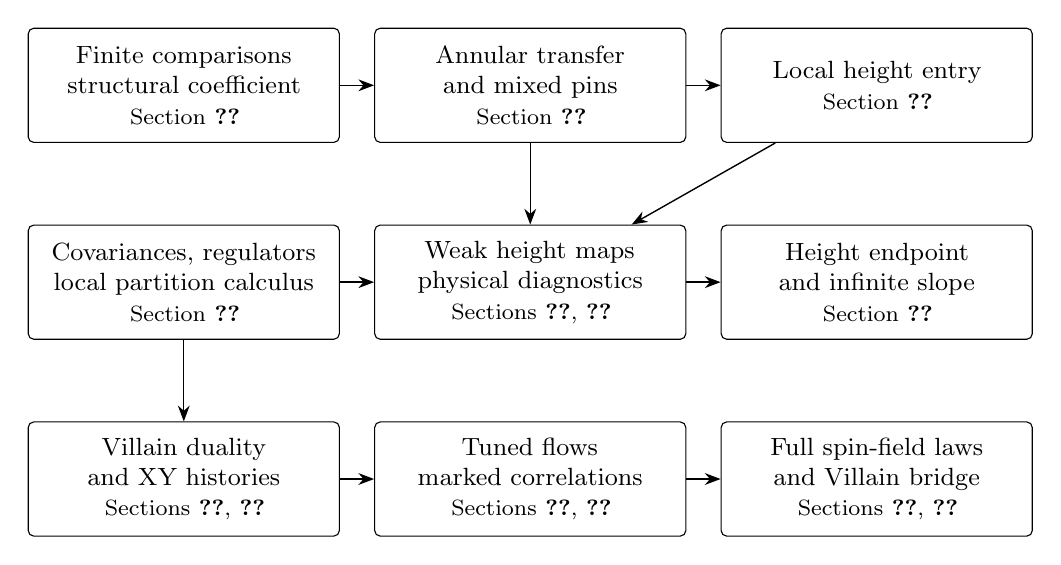
\begin{tikzpicture}[
 box/.style={draw,rounded corners=2pt,align=center,text width=3.6cm,
             minimum height=1.45cm,inner sep=5pt,font=\small},
 arr/.style={-{Stealth[length=2mm]},line width=.5pt}]
 \node[box] (struct) at (0,0) {Finite comparisons\\structural coefficient\\
   \footnotesize Section~\ref{st:section}};
 \node[box] (annular) at (4.4,0) {Annular transfer\\and mixed pins\\
   \footnotesize Section~\ref{an:section}};
 \node[box] (entry) at (8.8,0) {Local height entry\\
   \footnotesize Section~\ref{en:section}};
 \node[box] (toolkit) at (0,-2.5) {Covariances, regulators\\local partition calculus\\
   \footnotesize Section~\ref{rg:section}};
 \node[box] (weak) at (4.4,-2.5) {Weak height maps\\physical diagnostics\\
   \footnotesize Sections~\ref{wh:section}, \ref{ep:section}};
 \node[box] (endpoint) at (8.8,-2.5) {Height endpoint\\and infinite slope\\
   \footnotesize Section~\ref{ep:section}};
 \node[box] (spin) at (0,-5) {Villain duality\\and XY histories\\
   \footnotesize Sections~\ref{vi:section}, \ref{xyh:section}};
 \node[box] (marks) at (4.4,-5) {Tuned flows\\marked correlations\\
   \footnotesize Sections~\ref{vi:section}, \ref{xyf:section}};
 \node[box] (field) at (8.8,-5) {Full spin-field laws\\and Villain bridge\\
   \footnotesize Sections~\ref{vi:section}, \ref{xyf:section}};
 \draw[arr] (struct)--(annular);
 \draw[arr] (annular)--(entry);
 \draw[arr] (entry)--(weak);
 \draw[arr] (toolkit)--(weak);
 \draw[arr] (weak)--(endpoint);
 \draw[arr] (toolkit)--(spin);
 \draw[arr] (spin)--(marks);
 \draw[arr] (marks)--(field);
 \draw[arr] (annular.south)--(weak.north);
\end{tikzpicture}
\caption{Dependencies among the main arguments.  The upper route
identifies the physical height endpoint; the lower route controls spin
insertions and then their full distribution.  Arrows show dependencies,
not reading order: the local entry construction is presented after the
weak maps whose parameters it accepts, and supplies their physical
initial data for the endpoint argument.  The Villain bridge also uses
the high-temperature height result of Section~\ref{wh:section}, and the
endpoint odd-sector argument returns directly to the structural face
ratio in Section~\ref{st:section}.}
\label{main:dependencies}
\end{figure}

\clearpage
\tableofcontents
\clearpage
\section{Finite comparisons and the structural height coefficient}
\label{st:section}

The output of this section is a coefficient $a(k)$ determined by
Gaussian limits on free rectangles.  Finite lattice comparisons also
give the gap $a(k)=0$ or $a(k)\ge8\pi$, and localization on the zero
branch.  Section~\ref{an:section} will relate this coefficient to the
physical roughness threshold and to the field on other domains.

Throughout this section $J$ has the hypotheses in the introduction, $v=v_J$,
\begin{equation}\label{st:normalization}
 A_0=-\Delta_J/v^2,\qquad k=\beta/v^2,\qquad h=\sigma\in2\pi\Z.
\end{equation}
An unoriented interaction edge has conductance $c=(|J|v^2)^{-1}$; parallel
edges are counted with their multiplicities. Thus
$(g,A_0g)=\sum_e c(\nabla_e g)^2$, and the Fourier symbol of $A_0$ is
$|p|^2+O_J(|p|^4)$. Write $R_J=\max_{z\in J}|z|_\infty$.
For a finite rectangle $B$ retain only edges whose two endpoints belong to
$B$, and denote the resulting Laplacian and its inverse on constants'
orthogonal complement by $A_B$ and $G_B=A_B^+$. A free height law is the
probability law modulo common translations by $2\pi\Z$, with weight
$\exp\{-(h,A_Bh)/(2k)\}$. Pinning one vertex is one choice of representative.
All pairings on a finite graph are counting-measure pairings.

Here is a useful convention concerning errors. An edge representation
$X=\sum_e w_e\nabla_e h$ has \emph{flow cost}
$\sum_e w_e^2/c$. For a zero-sum vertex profile $f$,
\begin{equation}\label{st:flow}
 (f,G_Bf)=\min_{\operatorname{div}w=f}\sum_e w_e^2/c.
\end{equation}
Indeed the minimizer is $w=c\nabla G_Bf$; its difference from every other
admissible flow is orthogonal to gradients in the scalar product
$\sum_e w_e w'_e/c$. In particular a test of flow cost $\delta$ has variance
at most $k\delta$ and all its exponential moments have the corresponding
Gaussian bound, by Lemma~\ref{st:finite-gaussian}. Nearest-neighbor edges,
which are present by hypothesis, may always be used to construct trial flows.

\subsection{Finite lattice Gaussian inequalities}

We start from the lattice inequalities of
\citet[Theorem~2.1, Corollary~3.2, and Propositions~3.3 and~4.2]{RSD2017}
and derive the comparison and limiting forms used below, including
proofs to specify the directions.
For applications of these inequalities to integer-height depinning
and graph surgery, see \citet{AizenmanHarelPeledShapiro2022}.

\begin{lemma}[Finite Gaussian comparisons]\label{st:finite-gaussian}
Let $\mathcal L$ be a lattice in a finite-dimensional Euclidean space $E$,
let $V=\operatorname{span}\mathcal L$, and let $P_V$ be orthogonal projection
onto $V$. Suppose $T\ge0$ is symmetric and $T_V=P_VT|_V$ is positive
definite. For $x\in E$ set
$w_T(x)=\sum_{u\in\mathcal L+x}\exp\{-(u,Tu)/2\}$.
Then
\begin{equation}\label{st:lattice-inequality}
 w_T(0)^2w_T(x+y)w_T(x-y)\ge w_T(x)^2w_T(y)^2.
\end{equation}
The covariance of the Gaussian on $\mathcal L+x$ is at least that on
$\mathcal L$ at the same precision, in positive-semidefinite order; the
same lower bound holds after a real linear tilt of the shifted law. For
each fixed ambient displacement $x$, the ratio $w_{T+tB}(x)/w_{T+tB}(0)$
is nonincreasing in $t\ge0$ whenever $B\ge0$. For the centered Gaussian
$H$ on $\mathcal L$, every real linear test $X=(\ell,H)$ satisfies
\begin{equation}\label{st:mgf-sandwich}
 \tfrac12\Var(X)\le\log\E e^X
 \le\tfrac12(\ell_V,T_V^{-1}\ell_V),\qquad \ell_V=P_V\ell.
\end{equation}
Centered variances and real moment generating functions decrease when
precision increases. For any two real linear tests,
\begin{equation}\label{st:paired-cumulant}
 \kappa(X,X,Y,Y)
 =\E X^2Y^2-\E X^2\E Y^2-2(\E XY)^2\ge0.
\end{equation}
The centered characteristic function is strictly positive, and its logarithm
has Hessian everywhere at least its Hessian at zero.
These centered conclusions apply after added centered pins or equalities.
For free graphs they apply to real tests annihilating every released
constant. The centered characteristic function is strictly positive for
characters invariant under every released translation, and its logarithmic
Hessian comparison holds along directions annihilating those constants.
The probability of a specified collection of centered lattice equalities
increases under a positive-semidefinite increase of precision.
\end{lemma}

\begin{proof}
For $d\in\mathcal L/2\mathcal L$ put
$z_d(s)=\sum_{u\in d+2\mathcal L}e^{-(u+s,T(u+s))/4}$.
Coercivity on $V$ makes these sums and their derivatives locally uniformly
convergent for ambient shifts.
The bijection $(u,v)\mapsto(u+v,u-v)$ gives
\[
 w_T(x)w_T(y)=\sum_d z_d(x+y)z_d(x-y),\qquad
 \sum_d z_d(s)^2=w_T(0)w_T(s).
\]
Cauchy--Schwarz proves Equation~\eqref{st:lattice-inequality}.
Taking logarithms and differentiating twice in $y$ at zero gives
$D^2\log w_T(x)\ge D^2\log w_T(0)$. Direct differentiation of the sum gives
$D^2\log w_T(x)=-T+T\Cov_x(H)T$. Both covariances are supported on $V$.
Restricting the Hessian inequality to directions in $V$ and inverting $T_V$
there proves covariance minimality.

For $x_T=T_V^{-1}P_VTx$ and $u\in V$, completion of the square gives
\[
 (u+x,T(u+x))=(u+x_T,T_V(u+x_T))+c_T(x),\qquad
 c_T(x)=(x,Tx)-(x_T,T_Vx_T)\ge0.
\]
For fixed $x$ and $T_t=T+tB$, $B\ge0$, differentiation in the ambient
space gives
\[
 \frac{d}{dt}\log\frac{w_{T_t}(x)}{w_{T_t}(0)}
 =-\tfrac12\tr\bigl[B(\Cov_x(H)-\Cov_0(H)
                         +\E_xH\otimes\E_xH)\bigr]\le0.
\]
This derivative keeps the ambient displacement fixed and includes the
$T_t$-dependence of both $x_{T_t}$ and the normal scalar $c_{T_t}(x)$.
A real tilt by $\ell$ changes the effective displacement on $V$ to
$x_T-T_V^{-1}\ell_V$. Its covariance therefore still dominates the centered
covariance. For the centered law, integrating the Hessian of its logarithmic
moment generating function on the segment from $0$ to $\ell$ proves the
first inequality in Equation~\eqref{st:mgf-sandwich}; symmetry makes the
first derivative at zero vanish. Differentiating this logarithmic moment
generating function with respect to $T_t$ gives the same nonpositive
expression with the tilted covariance and mean. Differentiating the resulting
centered comparison twice at zero proves the variance comparison. The second
derivative at $s=0$ of $\Var_{sY}(X)\ge\Var_0(X)$ proves
Equation~\eqref{st:paired-cumulant}.

Let $\mathcal L^*$ be the dual lattice in $V$. Poisson summation on $V$ gives
\[
 w_T(x)=e^{-c_T(x)/2}C_{T_V}\sum_{q\in\mathcal L^*}
 e^{-2\pi^2(q,T_V^{-1}q)}e^{2\pi i(q,x_T)}\le w_T(0).
\]
Completion of the square now proves the upper bound in
Equation~\eqref{st:mgf-sandwich}. For the centered characteristic function,
the same summation gives the strictly positive formula
\[
 \E e^{i(\ell,H)}
 =\frac{\displaystyle\sum_{q\in\mathcal L^*}
 e^{-\frac12(2\pi q-\ell_V,T_V^{-1}(2\pi q-\ell_V))}}
 {\displaystyle\sum_{q\in\mathcal L^*}e^{-2\pi^2(q,T_V^{-1}q)}}>0.
\]
It is a shifted-to-centered partition ratio on the dual lattice.
Equation~\eqref{st:lattice-inequality} there proves the assertion about its
logarithmic Hessian.

A collection of centered equalities selects
$\mathcal L_E=\mathcal L\cap\bigcap_j\ker\ell_j$, a lattice in its span.
The restricted precision is coercive, so the preceding argument applies
directly to its conditional centered law. In particular the displayed dual
sum proves strict characteristic positivity there. This law is also the
dominated limit of the additional precisions
$t\sum_j\ell_j\otimes\ell_j$, $t\uparrow\infty$, which transfers the centered
comparisons with the original law.

For a free graph choose one representative $h_{x_0}=0$ on each connected
component. Its representative lattice has a span on which the massless graph
precision is coercive. The same dual formula directly proves strict
characteristic positivity on that centered law, and hence for its
translation-invariant characters. To compare a graph with a cut graph,
first add $\eta\Id$.
On a connected component choose representatives $h_{x_0}=0$ and sum its
common translation $2\pi j$. Completion of the square shows that this sum,
divided by $(2\pi\eta|B|)^{-1/2}$, tends to a constant independent of the
representative and is uniformly bounded for $0<\eta\le\eta_0$.
The remaining representative weight is bounded by a constant times its
massless weight and converges pointwise to it. Dominated convergence,
also after any fixed real tilt annihilating constants, transfers the
comparison inequalities.
The same argument applies to bounded observations invariant under common
$2\pi$ translations, a fact used below for phases.
Finally, for an equality event $E$, differentiate its probability along
$T+tB$ before taking any infinite-penalty limit. Its logarithmic derivative
is $\frac12\tr B(\Cov(H)-\Cov(H\mid E))\ge0$ by the just-proved centered
pin comparison; both means vanish by inversion symmetry. This proves the
last assertion, and dominated limits give its free-graph versions whenever
the event is invariant under the released translations.
\end{proof}

For later use, a consequence of the last Hessian assertion is worth recording.
Let $\phi$ be the centered characteristic function in
Lemma~\ref{st:finite-gaussian}, let $s$ be a base profile, and let $Y$ have
bare variance at most $V$. On a free graph take $s$ with integer total on
each released component and $Y$ with zero total on each. Then
\begin{equation}\label{st:coefficient-transfer}
 \sqrt{-\log\phi(s+tY)}
 \le\sqrt{-\log\phi(s)}+|t|\sqrt{V/2}.
\end{equation}
To prove this, set $f(t)=\log\phi(s+tY)\le0$. The inequality $f''\ge-V$
and the upper bound $f\le0$, applied at the maximum of
$f(t)+f'(t)u-Vu^2/2$, imply $|f'|^2\le-2Vf$.
Integration, or regularization at zeros of $-f$, gives
Equation~\eqref{st:coefficient-transfer}. In particular, a positive lower
bound transfers between profiles at bounded bare distance in either direction.

\subsection{Saturation on free rectangles}

Let $B_m=\{0,\ldots,m-1\}^2$, $g_m(x)=x_1/m$, and
\begin{equation}\label{st:am}
 a_m(k)=\Var_{B_m,k}(h,A_{B_m}g_m).
\end{equation}
The energy $(g_m,A_{B_m}g_m)$ tends to one, by square symmetry and the
definition of $v$. Thus $0\le a_m\le k+o(1)$.

\begin{theorem}[All free-rectangle limits]\label{st:free-rectangle-limit}
There is a number $a=a(k)\in[0,k]$ such that $a_m(k)\to a$.
Let $B_n$ be discrete axis rectangles at mesh $n^{-1}$ whose endpoints
converge to those of a fixed nondegenerate rectangle $B$. For every finite
collection of smooth shifts $g$ on a neighborhood of $\overline B$,
\begin{equation}\label{st:rectangle-laplace}
 \log\E_{B_n,k}\exp\{(h,A_{B_n}g(\cdot/n))\}
 \longrightarrow \frac a2\int_B|\nabla g|^2.
\end{equation}
The corresponding tests converge jointly to centered Gaussian variables
with covariance $a\int_B\nabla g\cdot\nabla g'$; all joint moments converge.
For zero-total profiles $f_n$ whose scaled piecewise constant densities
$n^2f_n$ converge in $L^2(B)$ to a bounded piecewise continuous $f$ of
integral zero, the corresponding assertion is
\begin{equation}\label{st:rectangle-smear}
 \log\E_{B_n,k}e^{(h,f_n)}
 \longrightarrow \frac a2(f,(-\Delta_{B,N})^{-1}f)_{L^2(B)}.
\end{equation}
Here the inverse Neumann Laplacian is on integral-zero functions. These
statements hold along every such sequence of rectangles and jointly for
mixed finite lists of the displayed tests.
\end{theorem}

\begin{proof}
We give separately the cutting, folding, and distributional steps.

\emph{Cutting and the existence of $a$.}
Cut a square of side $M$ into $m$-squares and strips of width less than $m$.
In its affine observation $x_1/M$, the squared cost of omitted seam and
strip flows is at most $C_J(m^{-1}+m/M)$: there are at most
$C_J(M^2/m+mM)$ affected edges and each coefficient is at most $C_J/M$.
On the remaining squares the observation is $m/M$ times the cell
observation. Cutting increases variance, and the cut components are
independent. The triangle inequality in $L^2$ consequently gives
\begin{equation}\label{st:cut-am}
 \sqrt{a_M}\le\sqrt{a_m}+C_J\sqrt{k}(m^{-1}+m/M)^{1/2}.
\end{equation}
First let $M\to\infty$, then take $m\to\infty$ along a liminf subsequence.
This proves convergence. Notice also that each $a_m(k)$ is continuous
for $k>0$, by locally uniform convergence of its defining Gaussian sums,
and Equation~\eqref{st:cut-am} is uniform when $k$ ranges over a compact
subset of $(0,\infty)$. In particular
$\sqrt{a(k)}\le\sqrt{a_m(k)}+C_J\sqrt{k/m}$.
Square symmetries make the covariance matrix of
the two affine tests scalar. Cutting a rectangle into small squares proves
the affine upper bound $a\int_B|\nabla g|^2$. For its reverse, let
$m_1(n),m_2(n)$ be the rectangle's side counts and set
$V_n(p)=\Var_{B_n}(h,A_{B_n}(p\cdot x/n))$. Tile a square of side $M$,
divisible by both side counts, with copies of this rectangle. The
normalized affine test $p\cdot x/M$ restricts on each cell to $n/M$
times the cell test, up to an irrelevant constant. There are
$M^2/(m_1(n)m_2(n))$ cells. Cutting and the seam-flow estimate, followed
by $M\to\infty$ at this fixed $n$, give
\[
 \sqrt a\,|p|
 \le\frac{n}{\sqrt{m_1(n)m_2(n)}}\sqrt{V_n(p)}
       +\frac{C_{J,k,p}}{\sqrt{\min(m_1(n),m_2(n))}}.
\]
Since $m_1(n)m_2(n)/n^2\to|B|$, this proves
$\liminf_nV_n(p)\ge a|p|^2|B|$ along every admissible rectangle sequence.
Together with the cutting upper bound it gives
\[
 \lim_n\Var_{B_n}(h,A_{B_n}g)=a\int_B|\nabla g|^2
\]
for every affine $g$ and every such sequence.

Cutting into cells of small fixed macroscopic diameter and replacing
$\nabla g$ by constants proves, for smooth or continuous piecewise smooth
$g$ with bounded piece derivatives and polygonal interfaces,
\begin{equation}\label{st:upper-energy}
 \limsup_n\Var(h,A_{B_n}g)\le a\int_B|\nabla g|^2.
\end{equation}
At a fixed partition the omitted edge count is $O(n)$ and coefficients
are $O(n^{-1})$, so their cost tends to zero. In cell interiors the error
cost is bounded by the $L^2$ modulus of continuity of the gradient, which
tends to zero as the partition is refined. The identical proof applies to
partial gradient observations restricted to polygonal pieces.

Call a shift $g$ saturated on $B$ if, for every admissible sequence
of discrete rectangles $B_n$ converging to $B$,
\[
 \lim_{n\to\infty}\Var_{B_n}(h,A_{B_n}g(\cdot/n))
       =a\int_B|\nabla g|^2.
\]
For a partial gradient observation use the same full-limit definition
with the energy integral over its retained region.

This class is linear. Fix a finite list of saturated shifts and any
admissible rectangle sequence. From any subsequence one can extract a
further subsequence on which their covariance matrix converges, by the
bare bounds. If $C$ is that limiting matrix and
$E_{ij}=a\int_B\nabla g_i\cdot\nabla g_j$, then
Equation~\eqref{st:upper-energy}, applied to every real linear combination,
gives $E-C\ge0$. Full convergence for each $g_i$ gives
$(E-C)_{ii}=0$ on this same subsequence. A positive-semidefinite matrix
with zero diagonal has all its entries zero. Thus $C=E$.
Since this applies to every initial subsequence, the covariance matrices
converge along the original sequence. In particular every finite linear
combination is saturated.

Saturation on a larger rectangle passes to an enclosed rectangle.
Partition the complement into finitely many rectangles, indexed together
with the inner rectangle by $i=0,\ldots,r$, and write
$E_i=\int_{B_i}|\nabla g|^2$. Vanishing seam-flow errors and cutting give
\[
 V_{\mathrm{outer},n}\le\sum_{i=0}^rV_{i,n}+o(1).
\]
The outer variance converges to $a\sum_iE_i$, while
$\limsup_nV_{i,n}\le aE_i$ for every piece. Consequently
\[
 \liminf_nV_{0,n}
 \ge a\sum_iE_i-\sum_{i=1}^r\limsup_nV_{i,n}
 \ge aE_0.
\]
Together with the upper bound this is full convergence on the inner
rectangle, on every admissible sequence. Strict enlargements suffice;
compatible rounding of the partition changes only vanishing-cost flows.

The class is also closed under gradient-energy approximation. If
$g_j$ are saturated and $\|\nabla(g_j-g)\|_{L^2(B)}\to0$, with convergence
of the corresponding discrete difference energies, then the bare bound
and the triangle inequality for standard deviations give
\[
 \limsup_n\left|
 \sqrt{\Var(h,A_{B_n}g)}-\sqrt a\,\|\nabla g\|_{L^2(B)}
 \right|
 \le(\sqrt k+\sqrt a)\|\nabla(g-g_j)\|_{L^2(B)}.
\]
Letting $j\to\infty$ proves full convergence for $g$. The same argument
shows that an observation changed by a flow of cost tending to zero
retains its full variance limit. These statements apply to the fixed
smooth and continuous piecewise smooth shifts used below, whose discrete
energies converge by Riemann summation.

\emph{The fold.}
We justify the FKG correlation input \citep{FKG1971} directly.
A quadratic attractive height
law has the lattice condition
$p(u\wedge v)p(u\vee v)\ge p(u)p(v)$, since it holds edge by edge for
$e^{-c(h_x-h_y)^2/(2k)}$. On a finite height box this condition implies
association by induction in the number of vertices. Conditional laws in
one fewer coordinate satisfy the same condition. Between two values of
the last coordinate the likelihood ratio of their conditional laws is
increasing. The induction hypothesis applied to that ratio proves that
the conditional expectation of every increasing function increases.
The conditional covariance decomposition and the one-variable identity
$\Cov(F(Z),G(Z))=\frac12\E[(F(Z)-F(Z'))(G(Z)-G(Z'))]\ge0$
complete the induction. Letting the box grow proves association in our
proper finite Gaussian law. This argument also proves association after
conditioning any set of vertices.

Suppose a rectangle and its discrete graph are invariant under reflection
across a site axis or diagonal. Pin a site of the reflection line and
condition its entire height trace. The conditional law remains invariant
under reflection and associated, including interactions crossing the line.
For a saturated shift odd about that line up to a constant, let $X_+$ and
$X_-$ be its observations on edges internal to the two open sides. Then
$X_-$ is the reflected negative of $X_+$ and their sum differs from the
full observation by a vanishing-cost flow. If $X_+$ can be changed by such
a flow to have nonnegative off-line vertex coefficients, conditional
association gives a nonpositive conditional covariance with $X_-$.
Their conditional means are negatives, so the unconditional covariance
is also nonpositive. Write $V_{\pm,n}=\Var(X_\pm)$ and
$E_\pm=\int_{B\cap\{\pm\text{ side}\}}|\nabla g|^2$.
The vanishing-cost modifications give
$\Cov(X_+,X_-)\le o(1)$, and the full observation differs from
$X_++X_-$ by a vanishing-cost flow. Its full variance convergence
therefore gives
\[
 a(E_++E_-)
 =\lim_n V_{\mathrm{full},n}
 \le\liminf_n(V_{+,n}+V_{-,n}).
\]
More directly, $V_{+,n}\ge V_{\mathrm{full},n}-V_{-,n}-o(1)$,
so the separate upper bound gives
\[
 \liminf_nV_{+,n}
 \ge a(E_++E_-)-\limsup_nV_{-,n}\ge aE_+.
\]
The same argument applies to the minus side. With
$\limsup_nV_{\pm,n}\le aE_\pm$, both partial variances converge
along the full sequence. The folded-shift observation differs from its
partial observation by a vanishing-cost flow, so it too has the required
full variance limit.

Here are the required coefficient checks and error bounds. For an axis
fold of $g=x_1$, pair each step $(z_1,z_2)$ with $(-z_1,z_2)$.
The coefficients of $A_{B_+}g$ vanish away from the two normal-face strips,
are nonpositive in the strip adjacent to the cut, and nonnegative at the
outer normal face. Tangential boundaries preserve this cancellation.
Move every cut-strip coefficient to the conditioned line along at most
$R_J+1$ nearest-neighbor edges. There are $O(n)$ coefficients of size
$O(n^{-1})$, and the paths have bounded overlap, giving cost $O(n^{-1})$.
Thus $(x_1-t)_+$ is saturated after coherent rounding of the reflection
line and restriction from an enclosing symmetric rectangle. Finite linear
combinations and gradient approximation give every smooth function of
either coordinate.

For the diagonal fold put $Y=y+t$ and use an enclosing square
$p\le x,Y\le q$. Take $g=F(x)-F(Y)$ with $F'''<0$ and
$F'(p),F'(q)>0$ on a slightly larger interval. In the interior of $x>Y$,
$A_Bg\ge0$: the symmetric second differences of $F$ decrease with their
center, and the step lists in the two coordinates coincide. At the outer
face $x=q$ the missing-step contribution has leading term a positive
constant times $F'(q)/n$; at $Y=p$ it has leading term a positive constant
times $F'(p)/n$. The tangential first-order terms cancel in pairs.
Uniform strict endpoint positivity absorbs the $O(n^{-2})$ remainder.
More precisely, in integer coordinates $P\le i,j\le Q$, the exceptional
sets can be taken as $D=\{0<i-j\le2R_J\}$ and
$K=\{Q-i\le R_J,\ j-P\le R_J\}$. Outside $D$ neither the lower $i$-face
nor the upper $j$-face truncates a step; outside $K$ the other two faces
cannot both truncate. This proves the stated sign everywhere outside
$D\cup K$. Move all coefficients in $D\cup K$ horizontally from $(i,j)$
to $(j,j)$ on the line. There are $O(n)$ short paths of length at most
$2R_J$ and $O(1)$ paths of length $O(n)$, with bounded overlap.
Their coefficients have size $O(n^{-1})$. If the overlap is $M$, their
cost is at most $(M/c)\sum_v d(v)^2|P_v|=O(n^{-1})$.
Define the opposite-side modification by reflected negative, so the
line terms cancel exactly. The fold criterion proves
saturation of
\begin{equation}\label{st:diagonal-fold}
 (F(x)-F(y+t))\ind_{\{x>y+t\}}.
\end{equation}
Every smooth $F$ on the fixed interval is a difference of two functions
with the strict properties just used: add a sufficiently large fixed
cubic with negative third derivative, and then a sufficiently large
positive linear function. Thus Equation~\eqref{st:diagonal-fold} is
saturated for arbitrary smooth $F$.

For clarity, coherent rounding preserves these full limits. Choose
$t_n=r_n/n$ with $r_n=\operatorname{round}(nt)$, and enclose the target
rectangle in the exactly symmetric lattice square
$P_n\le i\le Q_n$, $P_n-r_n\le j\le Q_n-r_n$.
Its reflection is $(i,j)\mapsto(j+r_n,i-r_n)$, and its scaled endpoints
can be chosen to converge. The odd seed $F(x)-F(y+t_n)$ differs from the
fixed saturated seed $F(x)-F(y+t)$ by discrete gradient energy
$O(|t_n-t|^2)$. For the folded functions $f_{t_n},f_t$ of
Equation~\eqref{st:diagonal-fold}, the squared difference energy is at most
$C(|t_n-t|+n^{-1}+|t_n-t|^2)$. Indeed the strip between their diagonals,
enlarged by $R_J/n$, meets $O(n^2|t_n-t|+n)$ edges, each carrying an
$O(n^{-1})$ difference increment; away from it, smooth derivative
differences are $O(|t_n-t|)$. Axis hinges satisfy the same estimate.
Thus the fold and restriction limits transfer to each fixed target
shift along every admissible rectangle sequence by the vanishing-cost
perturbation bound.

To see that these folds suffice, extend a smooth target $g$ slightly and
choose a smooth family $F_t$ of compact support in $t$, on all relevant
parameters, satisfying $F_t'(x)=-g_{xy}(x,x-t)$. Differentiating the integral
of Equation~\eqref{st:diagonal-fold} gives
\[
 \partial_x\partial_y\int
 (F_t(x)-F_t(y+t))\ind_{\{x>y+t\}}\,dt=-F_{x-y}'(x)=g_{xy}(x,y).
\]
The residual is a sum of two univariate functions. Riemann sums of this
integral converge in gradient $L^2$: translations of the bounded piecewise
smooth gradients are continuous in $L^2$, including across the moving
diagonal. The bare bound then transfers saturation to $g$.

\emph{Laplace transforms and smears.}
The lower bound in Equation~\eqref{st:rectangle-laplace} follows from
saturation and Equation~\eqref{st:mgf-sandwich}. For the upper bound, cut
into cells of side comparable to a small fixed $r$. For fixed $r$, the
discarded-flow observation $E_n$ has bare variance tending to zero.
H\"older with exponents $p>1$ and $p/(p-1)$ removes $E_n$ at a cost tending
to zero. Precision comparison bounds the remaining log transform by the
sum of independent cell log transforms with argument $p$. Each cell
variable has bare variance $O(r^2)$, so its subGaussian bound gives
\[
 \log\E e^{pX}=\tfrac12p^2\Var X+O_p(r^3),
\]
uniformly in the fine mesh. For example Taylor's integral remainder is
bounded by $C_p\E[|X|^3e^{p|X|}]=O_p(r^3)$ using the Gaussian tail.
There are $O(r^{-2})$ cells. Apply Equation~\eqref{st:upper-energy}, let
$n\to\infty$, then $r\downarrow0$, then $p\downarrow1$. This proves the
matching upper bound. Apply it to arbitrary linear combinations to obtain
the joint law; the uniform exponential bounds give convergence of moments.

Finally nearest-neighbor Poincar\'e gives
$\|u-\bar u\|_2^2\le C_Bn^2(u,A_{B_n}u)$. Consequently the bare variance
of a density error is bounded by its scaled $L^2$ norm squared. Approximate
$f$ by finitely many nonconstant Neumann cosines of the rectangle, and
use their smooth inverse-Laplacian shifts. For a Neumann shift,
$n^2A_{B_n}g$ converges in density $L^2$ to $-\Delta g$: interior errors
vanish by Taylor expansion; boundary coefficients are $O(n^{-2})$ because
the normal derivative vanishes and tangential steps cancel. At corners
both derivatives vanish. The $O(n)$ boundary-layer sites have vanishing
scaled area, so their bounded scaled errors disappear. Use the actual
discrete rectangle endpoints in this approximation and then let them
converge. Poincar\'e and bare domination complete the density approximation
and prove Equation~\eqref{st:rectangle-smear} and its joint version.
\end{proof}

A face probability can also be used in the zero-total smear conclusions.
Replacing it by a uniform strip of width $r$ costs at most $C_Jr+O(n^{-1})$:
send each row's mass normally over distance at most $rn$ with currents
$O(n^{-1})$. Apply Theorem~\ref{st:free-rectangle-limit} at fixed $r$ and
then let $r\downarrow0$. In particular, differences of face and volume
probabilities have bounded bare cost, and have variance tending to zero
when $a=0$.
\subsection{Neutral charges and the fractional mean}

For a free graph, $w_B(s)=\E e^{i(h,s)}$ is well defined independently of
the representative whenever $\sum_xs_x\in\Z$. Pin a vertex $o$ and apply
Poisson summation in the remaining $2\pi\Z$ coordinates. Extending a
residual profile by its opposite sum at $o$ identifies its quadratic form
with the free inverse-Laplacian form. The result is the exact identity
\begin{equation}\label{st:poisson-charge}
 w_B(s)=
 \frac{\displaystyle\sum_{q\in\Z^B:\,\sum q=\sum s}
       e^{-\frac k2(q-s,G_B(q-s))}}
      {\displaystyle\sum_{q\in\Z^B:\,\sum q=0}
       e^{-\frac k2(q,G_Bq)}}\in(0,1].
\end{equation}
There is no $2\pi$ in the dual energy, because the height spacing is $2\pi$.
Let $\nu_B$ be the centered neutral charge law in the denominator. Twice
differentiating Equation~\eqref{st:poisson-charge} at $s=0$ in directions
$A_Bg,A_Bg'$ gives
\begin{equation}\label{st:dual-covariance}
 \Cov_{\nu_B}((q,g),(q,g'))
 =k^{-1}(g,A_Bg')-k^{-2}\Cov_B((h,A_Bg),(h,A_Bg')).
\end{equation}
At an arbitrary integer-total profile, one differentiation gives
\begin{equation}\label{st:dual-mean}
 \partial_{A_Bg}\log w_B(s)
       =k(g,\E_s(q-s)).
\end{equation}
The dual Gaussian comparison implies that the Hessian of $\log w_B$ in
neutral directions is at least its centered Hessian, namely minus the
height covariance. Equation~\eqref{st:coefficient-transfer} applies here.

We will also use the following replica identity, with no limiting assumption.
For two independent centered height copies let $S=h_1+h_2$ and $D=h_1-h_2$.
Condition on their common parity class modulo $4\pi\Z$ after pinning.
Then $S,D$ are conditionally independent and identically distributed,
each with half the original precision. For linear tests $i,j$, put
$V_{ij}=\E[S_iS_j\mid\text{parity}]$. Expansion of the two independent
copies gives
\begin{equation}\label{st:replica-covariance}
 \E V_{ij}=2\Cov(h_i,h_j),\qquad
 \Cov(V_{ij},V_{rs})=2\kappa(h_i,h_j,h_r,h_s).
\end{equation}
Indeed $\E[V_{ij}V_{rs}]=\E[S_iS_jD_rD_s]$ by conditional independence;
the terms with an odd number of factors from either copy vanish, and the
remaining terms are $2\E[h_ih_jh_rh_s]+2C_{ij}C_{rs}
-2C_{ir}C_{js}-2C_{is}C_{jr}$. Subtract $4C_{ij}C_{rs}$.

\begin{theorem}[Uniform fractional mean]\label{st:fractional-mean}
Suppose $a(k)>0$, and let $u_m$ be the uniform probability on $B_m$.
Then $(h,u_m)$ modulo $2\pi$ converges to uniform measure on the circle,
independently of the Gaussian observations in
Theorem~\ref{st:free-rectangle-limit} on a square. More generally, for every
fixed $l\in\Z\setminus\{0\}$ and every sequence of zero-total profiles
$t_m$ of uniformly bounded bare inverse energy,
\begin{equation}\label{st:vanishing-phase}
 w_{B_m}(lu_m+t_m)\longrightarrow0.
\end{equation}
\end{theorem}

\begin{proof}
Write $g_m=(x_1-(m-1)/2)/m$, $X=(h,A_Bg_m)$, and
$Y=(h,\rho-u_m)$, where $\rho$ is the uniform right-face probability.
The flow bound makes $Y$ uniformly subGaussian. Reflection changes $X$
to $-X$ and exchanges right and left faces, so
\begin{equation}\label{st:face-covariance}
 \Cov(X,Y)\longrightarrow a/2.
\end{equation}
Here is a discrete verification of the normalization. The profile
$A_Bg_m$ is supported in fixed-width side layers. Except in boundedly many
corner sites, its right-layer row sums are constant, its left-layer row
sums are their negatives, and all other sums vanish, by pairing steps.
Transport these coefficients to their respective faces along bounded
paths; the cost is $O(m^{-1})$. Corner discrepancies of size $O(m^{-1})$
can be routed along $O(m)$ paths, at cost $O(m^{-1})$. Thus
$A_Bg_m-t_m(\rho_R-\rho_L)$ has vanishing flow cost. Pairing with $g_m$
and using $(g_m,A_Bg_m)\to1$ gives $t_m\to1$. This proves
Equation~\eqref{st:face-covariance}.

Fix $l\ne0$ and suppose along a subsequence
$w_B(lu_m)\to r>0$. Uniform subGaussian bounds on $X,Y$ allow a further
subsequence on which
\[
 F_m(t,u)=\E\exp\{il(h,u_m)+itX+iuY\}
\]
converges locally uniformly with all derivatives on $\C^2$.
This follows from the uniform bound
$|F_m(t,u)|\le\E e^{|\Im t||X|+|\Im u||Y|}$, Cauchy's formula, and a
diagonal Arzel\`a--Ascoli argument. The limit $F$ is real and nonnegative
on $\R^2$ by Equation~\eqref{st:poisson-charge}.

The Gaussian limit and moment convergence of $X$ imply
$\Var(V_{XX})=2\kappa(X,X,X,X)\to0$. The fourth moments of $Y$ are bounded,
so $\Var(V_{YY})$ is bounded. By Equation~\eqref{st:replica-covariance},
\[
 \Var(V_{XY})=2\kappa(X,X,Y,Y)
            =\Cov(V_{XX},V_{YY})\longrightarrow0.
\]
Multiply $V_{XX}$ or $V_{XY}$ by the conditional characteristic function
of $D$ with phase $l\bar D+tD_X+uD_Y$. Its modulus is at most one, so the
concentration just proved and conditional independence permit replacement
of $V_{ij}$ by $2C_{ij}$. Direct expansion in the two original copies gives
\[
 \E[S_iS_j e^{i(l\bar D+tD_X+uD_Y)}]
       =-2(F_m F_{m,ij}-F_{m,i}F_{m,j}).
\]
Since $\E e^{i(l\bar D+tD_X+uD_Y)}=F_m^2$, it follows wherever $F>0$ that
$(\log F)_{tt}=-a$ and $(\log F)_{tu}=-a/2$.
At $(0,0)$ reflection gives $F_t=0$. Analytic continuation yields
\begin{equation}\label{st:phase-transform}
 F(t,u)=F(0,u)\exp\{-at^2/2-atu/2\}.
\end{equation}
Equation~\eqref{st:coefficient-transfer} ensures $F(0,l)>0$, because the
bare cost of $lY$ is bounded.

Now join two horizontally adjacent $m$-squares to form a free rectangle,
and use its centered neutral charge law. For a charge $q$, let $Q$ be its
left total, the right total being $-Q$. Use the following trial quadratic
form: in each cell route the residual $q-Q_B\rho_B$ with its minimizing
internal flow, where $\rho_B$ is its seam-face probability; route $Q$
uniformly across the $m$ nearest-neighbor seam edges; add the penalty $Q^2$.
The resulting form is
\[
 k\sum_{B=L,R}(q_B-Q_B\rho_B,G_B(q_B-Q_B\rho_B))+D_mQ^2,
 \qquad D_m=1+k/(cm).
\]
It dominates the actual precision form $k(q,Gq)$ by
Equation~\eqref{st:flow}. Conditional on $Q$, the trial cells are independent
shifted neutral lattice Gaussians, whose affine variances dominate the
centered ones. By Equation~\eqref{st:dual-covariance} and saturation, their
sum tends to $2(k-a)/k^2$, exactly the actual variance of the global affine
test $x_1/m$ on the two-cell rectangle. Precision comparison gives the
opposite upper bound for the trial total variance. Thus the variance,
over $Q$, of its conditional affine mean tends to zero.

The sector weights, after common normalization, are
$e^{-D_mQ^2/2}w_L(Q\rho_L)w_R(-Q\rho_R)$.
Their normalizing sum is at most $\sum_Q e^{-Q^2/2}$ and the $Q=0$ term is
one. The $Q=l$ term stays positive by Equation~\eqref{st:coefficient-transfer}.
In that sector Equation~\eqref{st:dual-mean} and
Equation~\eqref{st:phase-transform} give
$k(g,\E[q-l\rho])\to-al/2$ in the left cell. Reflection and charge
reversal give the same residual pairing in the right cell. The two
seam-face contributions to the global affine mean differ by only
$O(m^{-1})$. Its $Q=l$ conditional mean therefore tends to $-al/k\ne0$,
whereas the $Q=0$ conditional mean is zero. This contradicts the vanishing
sector-mean variance. Thus $w_B(lu_m)\to0$.

If Equation~\eqref{st:vanishing-phase} failed, its positive lower bound
would transfer to $lu_m$ by Equation~\eqref{st:coefficient-transfer}, which
is impossible. Joint convergence with the Gaussian observations follows
by Fourier polynomials on the circle and joint characteristic functions;
tightness on the circle and the already proved Gaussian tightness make
this convergence of the full joint law. Exponential bounds extend the
joint assertion to moments of the Gaussian coordinates.
\end{proof}

\subsection{The charge gap and a uniform critical-scale ratio}

Let $\rho_{B,e}$ be uniform probability on face $e$ of a square, and set
$\bar\rho_B=\frac14\sum_e\rho_{B,e}$ and
$z_m=w_{B_m}(\bar\rho_{B_m})>0$.

\begin{lemma}[Face ratio with a common constant]\label{st:critical-face-ratio}
Fix $J,k$. Suppose every fixed nonzero integer-total bounded face profile
has characteristic coefficient tending to zero as the square side tends
to infinity. This hypothesis holds if $a(k)>0$. There are constants
$c_*=c_*(J,k)>0$ and an integer $G_0$, independent of $G$, such that for
\emph{every fixed integer} $G\ge G_0$,
\begin{equation}\label{st:face-ratio}
 \liminf_{m\to\infty}\frac{z_{Gm}}{z_m}
       \ge c_*G^{\,2-a(k)/(4\pi)}.
\end{equation}
The fine-size threshold implicit in this liminf may depend on $G$.
At $a(k)=8\pi$, the same positive lower bound $c_*$ therefore holds
for arbitrarily large fixed $G$.
\end{lemma}

\begin{proof}
Tile the $Gm$-square into $G^2$ cells $B_i$. The restriction of the large
square's face probability to $B_i$ has total $\xi_i$ and equals the sum of
its exterior-face probabilities with coefficient $1/(4G)$ per exterior
face. Thus $\xi$ is supported on boundary cells, $\sum_i\xi_i=1$, and
$\sum_i\xi_i^2\le C/G$.
For a neutral real profile $r$, let $Q_i=\sum_{B_i}r$ and choose a linear
map from $Q$ to an antisymmetric nearest-neighbor coarse flow $F$ satisfying
$\operatorname{div}F=Q$ and zero exterior flux. The quadratic form
\begin{equation}\label{st:trial-precision}
 \begin{split}
 \mathcal T_m(r)={}&k\sum_i
 \left(r_i-\sum_eF_{ie}\rho_{i,e},
 G_{B_i}\left(r_i-\sum_eF_{ie}\rho_{i,e}\right)\right)\\
 &+\frac{k}{cm}\sum_{\langle i,j\rangle}F_{ij}^2+\sum_iQ_i^2
 \end{split}
\end{equation}
is at least $k(r,G_{B_{Gm}}r)$: use the internal minimizing flows and
send each coarse flux uniformly across the $m$ nearest-neighbor seam
edges. The last term is an extra positive penalty. The internal and seam
edges are disjoint, so their costs add. The form is positive definite on
the neutral space because zero cost forces $Q=0$ and then $r=0$.

In the numerator of Equation~\eqref{st:poisson-charge} take
$r=q-\bar\rho_{B_{Gm}}$; in the denominator take $r=q$. Precision
monotonicity of a shifted-to-centered ratio shows that replacement by
$\mathcal T_m$ gives a lower bound for $z_{Gm}$.
Sum this new partition function by integer cell totals $n_i=\sum_{B_i}q$.
Then $Q=n-\xi$ in the numerator and $Q=n$ in the denominator.
Divide both sums by the product of the cells' centered neutral partition
functions. Their internal factors become $\prod_iw_{B_i}(s_i)$, where
\[
 s_i=\sum_eH_{ie}\rho_{i,e},\qquad
 H_{ie}=\begin{cases}
 F_{ie},&\text{internal face},\\
 1/(4G),&\text{exterior face in the numerator},\\
 0,&\text{exterior face in the denominator}.
 \end{cases}
\]
In the denominator exterior $H$ is zero. In either case $\sum_eH_{ie}=n_i$.
All these factors lie in $(0,1]$. The penalty
$\exp(-\frac12\sum_iQ_i^2)$ is summable over the finite-rank integer sector
lattice, uniformly in $m$. Thus dominated convergence is valid at every
fixed $G$. Each nonzero denominator sector contains a nonzero integer-total
face profile and tends to zero by hypothesis. The zero sector equals one,
so the normalized denominator tends to one.

Keep numerator sectors $n=e_{i_0}$ with $i_0$ at distance at least $G/4$
from the boundary. Write $Y_i=s_i-n_i\bar\rho_{B_i}$. The logarithmic Hessian
bound for $w$ gives
\begin{equation}\label{st:face-product}
 \prod_iw_{B_i}(s_i)
 \ge z_m\exp\left\{-\tfrac12\sum_i\Var_{B_i}(h,Y_i)\right\}.
\end{equation}
For the linear term at zero, inversion symmetry suffices. On the total-one
hyperplane put
$\Psi_B(H)=\log w_B(\sum_eH_e\rho_{B,e})$, where $\sum_eH_e=1$.
Equation~\eqref{st:poisson-charge} makes this function smooth there, and
square symmetry makes its differential at $H_0=(1/4,1/4,1/4,1/4)$
invariant under the square group. Every tangent vector with zero coordinate
sum has group average zero, so this differential vanishes on it. The face
coefficients of each $Y_i$ have zero sum, and $n=e_{i_0}$ uses only the
base profiles zero and $\bar\rho_{B_i}$.

Put $D_{ij}=(H_{i,+j}-H_{i,-j})/2$ and
$S_{ij}=H_{i,+j}+H_{i,-j}$. Reflection in each coordinate splits $Y_i$ into
two odd face differences and an even remainder. These three pieces have
zero mutual covariance by symmetry. The odd differences have limiting
variance $a$ and zero cross covariance, as in
Equation~\eqref{st:face-covariance}; the even remainder has a bounded bare
variance times $\sum_jS_{ij}^2$, by the face-to-strip flow estimate.
Consequently, for fixed $G$ and fixed face coefficients,
\begin{equation}\label{st:face-energy-bound}
 \limsup_m\sum_i\Var(h,Y_i)
 \le a\sum_{i,j}D_{ij}^2+C_{J,k}\sum_{i,j}S_{ij}^2.
\end{equation}

We construct one coarse flow for each retained sector with bounds uniform
in $G,i_0$. In the continuum square of side $G$, let $x_0$ be the center
of cell $i_0$. There is a vector field with divergence $\delta_{x_0}$ and
constant outer normal flux $1/(4G)$, of the form
\begin{equation}\label{st:radial-flow}
 V(x)=\frac{x-x_0}{2\pi|x-x_0|^2}+E(x),\qquad
 |E(x)|\le C/G,\quad |\nabla E(x)|\le C/G^2.
\end{equation}
For completeness, subtract the expanding field
$(x-x_{\rm center})/(2G^2)$, which has divergence $G^{-2}$ and the desired
boundary flux. Solve the resulting zero-Neumann problem by even reflection
to the torus of side $2G$. After rescaling to a fixed torus, subtract
cutoff logarithms around its finitely many reflected poles. Their mutual
separations and distances from the original boundary are bounded below,
uniformly for $x_0/G$ in the central square. The remainder solves a smooth
mean-zero Poisson equation with uniformly bounded derivatives. Its Fourier
series has coefficients $\widehat f(p)/|p|^2$; repeated integration by
parts gives summability after any fixed number of differentiations.
This proves the smooth bounds in Equation~\eqref{st:radial-flow}, including
up to the reflected boundary. Adding back the expanding field proves the
assertion.

Integrate $V$ over the faces of each continuum unit cell, with outward
sign, to define $H$. It has divergence $e_{i_0}$ and the prescribed exterior
flux. The central faces have bounded fluxes. Off the central cell,
\[
 |S_{ij}|\le C(1+|i-i_0|)^{-2}+C/G^2,
 \qquad D_{ij}=V_j(i)+O((1+|i-i_0|)^{-2}+G^{-2}).
\]
Hence
\begin{equation}\label{st:radial-cost}
 \sum_{i,j}S_{ij}^2\le C,\qquad
 \sum_{i,j}D_{ij}^2\le\frac1{2\pi}\log G+C.
\end{equation}
The coefficient follows by integrating the squared radial field:
$\int_1^{CG}(4\pi^2r^2)^{-1}2\pi r\,dr=(2\pi)^{-1}\log G+O(1)$.
The comparison of the sum and integral has summable derivative error.
The cross term with $E$ is $O(G^{-1}\sum_{r\le CG}1)=O(1)$, and
$\sum|E|^2=O(1)$. All constants are uniform for the retained cells.
The internal part $F$ has divergence $e_{i_0}-\xi$. These vectors, for
central $i_0$, are linearly independent because their central coordinates
are distinct and $\xi$ is supported at the boundary. Prescribe the linear
flow map on them by this construction and extend it to a basis of the
neutral coarse space, using any path flow on the remaining basis vectors.
Thus a single quadratic form~\eqref{st:trial-precision} serves all retained
sectors; separate nonlinear choices of precision have not been made.

For these sectors the penalty $\|e_{i_0}-\xi\|_2^2$ is bounded by a common
constant. The crossing cost tends to zero as $m\to\infty$ for each fixed
$G$. Equations~\eqref{st:face-product}--\eqref{st:radial-cost} therefore give
at least $c z_mG^{-a/(4\pi)}$ from each sector in the liminf of the ratio.
There are at least $c'G^2$ retained sectors. Division by the denominator,
which tends to one, proves Equation~\eqref{st:face-ratio}, with one positive
constant for all $G\ge G_0$.
\end{proof}

\begin{corollary}[Exact forbidden range]\label{st:charge-gap}
For every admissible $J$ and $k>0$,
\begin{equation}\label{st:gap}
 a(k)=0\quad\hbox{or}\quad 8\pi\le a(k)\le k.
\end{equation}
\end{corollary}

\begin{proof}
If $0<a<8\pi$, Theorem~\ref{st:fractional-mean} gives the hypothesis of
Lemma~\ref{st:critical-face-ratio}. Choose a fixed $G$ so large that its
right side exceeds two. The definition of liminf then gives
$z_{Gm}\ge\frac32z_m$ for all sufficiently large $m$. Iteration along
$m,Gm,G^2m,\ldots$ contradicts $0<z_m\le1$. The upper bound $a\le k$ was
proved in Theorem~\ref{st:free-rectangle-limit}.
\end{proof}

\subsection{Localization when the structural coefficient vanishes}

\begin{proposition}[Zero coefficient implies localization]\label{st:zero-localization}
If $a(k)=0$, there is a finite constant $C_{J,k}$ such that
\begin{equation}\label{st:localized-criterion}
 \sup_{R\ge1}\E_{\mu^0_{J,v^2k,R}}h_0^2\le C_{J,k}.
\end{equation}
Moreover, there is a fixed integer $m\ge1$ for which centered height
laws on every sufficiently large square torus of side divisible by $m$
satisfy $\sup_{x,y}\E(h_x-h_y)^2\le C_{J,k,m}$.
\end{proposition}

\begin{proof}
\emph{Good phases at arbitrarily large scales.}
Some nonzero mean Fourier coefficient stays positive along a subsequence.
Otherwise $w_{B_m}(ju_m)\to0$ for all $j\ne0$. Every fixed face profile of
integer total $j$ differs from $ju_m$ by a test of variance tending to
zero, by the face extension of Theorem~\ref{st:free-rectangle-limit} at
$a=0$. The inequality
$|\E e^{iU}-\E e^{iV}|\le\sqrt{\E(U-V)^2}$ would then give the hypothesis
of Lemma~\ref{st:critical-face-ratio} with $a=0$, whose growth contradiction
is impossible. Hence along a subsequence, extracted diagonally over $j$,
\[
 w_{B_m}(ju_m)\longrightarrow r_j=r_{-j}\ge0,
 \qquad r_0=1,\qquad r_l>0\quad\text{for some }l\ge1.
\]

Use Equation~\eqref{st:trial-precision} on a $Gm$-square, now with shift
$l u_{Gm}$ instead of the face probability. Cell totals are
$Q_i=n_i-l/G^2$ in numerator sectors, with $\sum_i n_i=l$, and $Q_i=n_i$
in denominator sectors. For each fixed $G$ and sector, the crossing cost
vanishes as $m\to\infty$. The internal shifted profile differs from
$n_i u_m$ by a fixed linear combination of face and volume probabilities
of total zero, so its coefficient tends to $r_{n_i}$. The quadratic
penalty gives summable domination of the sector sums, exactly as in
Lemma~\ref{st:critical-face-ratio}. Therefore, with $b(j)=r_je^{-j^2/2}$,
\begin{equation}\label{st:phase-amplification}
 \liminf_m w_{B_{Gm}}(lu_{Gm})
 \ge e^{l^2/(2G^2)}\frac{b^{*G^2}(l)}{b^{*G^2}(0)}.
\end{equation}
The ratio on the right tends to one as $G\to\infty$. Here is a direct
local limit argument. Normalize $b$ to a probability $p$. It is even, has
exponential tails, positive mass at zero, and positive variance since
$p(l)>0$. Let $d\Z$ be its support subgroup; then $l\in d\Z$. Its
characteristic function $\psi$ has modulus less than one away from the
finitely many points $2\pi j/d$ in a period: equality in the triangle
inequality, together with $p(0)>0$, requires all support phases to equal
one. Near each such point,
$\psi(t)=1-\frac12\sigma^2(t-t_0)^2+O(|t-t_0|^4)$.
Fourier inversion of $\psi(t)^N e^{-ilt}$, splitting into fixed small
neighborhoods of these points and their complement, gives
$p^{*N}(l)=d(2\pi N\sigma^2)^{-1/2}(1+o(1))$, and the same formula at zero.
The complement is exponentially small, and the neighborhood calculation
uses $u=\sqrt N(t-t_0)$ with a Gaussian dominating bound. This proves the
ratio claim. Choose $G$ first and then arbitrarily large members $m$ of
the subsequence in Equation~\eqref{st:phase-amplification}. We obtain
arbitrarily large scales at which $w(lu)$ is arbitrarily close to one.

\emph{A joint phase bound.}
Fix $0<d_0<\pi/10$. Tile a torus by $m$-squares, with averages $\bar h_i$.
For any $\epsilon>0$ we can choose one of the preceding good scales so
that, for every collection $I$ of distinct cells,
\begin{equation}\label{st:phase-bad}
 \Prob\{\dist(l\bar h_i,2\pi\Z)\ge d_0\text{ for all }i\in I\}
 \le\epsilon^{|I|},
\end{equation}
uniformly in the number of torus cells. We provide the comparison that
makes this a joint, rather than single-cell, assertion.
Add independent $N(0,s^2)$ noises to the phases and wrap them modulo
$2\pi$. Let $p_T(y)$ be the resulting joint density. Expanding the wrapped
normal introduces integers $j_i$ and the quadratic costs
$\sum_i(y_i+2\pi j_i-l\bar h_i)^2/(2s^2)$.
Together with the height energy these are a lattice Gaussian on the
height and $j$ coordinates, shifted only in the $j$ coordinates. Add a
small centered height mass to make it positive definite.
Increasing the height precision from the cut free cells to the torus
therefore decreases $p_T(y)/p_T(0)$ by
Lemma~\ref{st:finite-gaussian}. Let the mass decrease to zero using the
translation-invariant clause of that lemma. This yields
\[
 \frac{p_T(y)}{p_T(0)}\le\prod_{i\in I}\frac{p_i(y_i)}{p_i(0)}.
\]
The wrapped-noise supremum bounds $p_T(0)\le(C/s)^{|I|}$.
Fourier positivity in Equation~\eqref{st:poisson-charge} bounds
$p_i(0)\ge(2\pi)^{-1}$. At a good scale the free-cell phase is within any
fixed small distance of zero with probability arbitrarily close to one:
use $\E\cos(l\bar h)=w(lu)$ and
$1-\cos x\ge1-\cos\delta$ when $\dist(x,2\pi\Z)\ge\delta$.
Thus, for the noisy free-cell phase,
\[
 \Prob\{\dist(l\bar h+Z,2\pi\Z)\ge d_0/2\}
       \le C e^{-c d_0^2/s^2}+\delta_m,
 \qquad \delta_m\longrightarrow0
\]
along increasingly good scales. Integrate the density-ratio bound over
the product of these bad sets. Conditional on original phases which are
all bad at threshold $d_0$, the independent noises retain badness at
threshold $d_0/2$ with probability at least
$\Prob(|Z|\le d_0/2)^{|I|}$. Hence the left side of
Equation~\eqref{st:phase-bad} is at most
\[
 \left[
 \frac{C}{s\Prob(|Z|\le d_0/2)}
       \bigl(e^{-c d_0^2/s^2}+\delta_m\bigr)
 \right]^{|I|}.
\]
Choose $s$ small first, then a sufficiently good large scale. This proves
Equation~\eqref{st:phase-bad} with the stated uniformity.

\emph{Neighbor differences and bad animals.}
Declare a coarse cell bad if its phase is bad, or if its average differs
from any axis-neighbor average by more than $d_0/l$.
For any list of $q$ pairs of neighboring cells with mutually disjoint
end cells, precision comparison after cutting into pair rectangles gives,
for each choice of signs $\eta_j\in\{-1,1\}$,
\[
 \E\exp\left\{T\sum_{j=1}^q\eta_j
                   (\bar h_{i_j}-\bar h_{i'_j})\right\}
 \le e^{q\delta_m(T)},\qquad \delta_m(T)\longrightarrow0.
\]
The free pair difference is a zero-total bounded density test, so the
limit follows from Equation~\eqref{st:rectangle-smear} at $a=0$; the bound
is uniform in the pair's location and orientation. Chernoff and the
$2^q$ sign choices give a bound
$[2e^{-Td_0/l+\delta_m(T)}]^q$ for simultaneous failures. Choose $T$ large
first and $m$ large afterward. This exponential base can thus be made as
small as desired, simultaneously with Equation~\eqref{st:phase-bad}.

For a prescribed sup-norm-connected set of $j$ coarse sites, assign each
bad site one of its five failure types (phase or one of four directed
neighbors). One type occurs at least $j/5$ times. For an edge type, a
greedy extraction gives at least $j/C_0$ mutually disjoint pairs, since
each pair meets only a bounded number of pairs of the same type. For the
phase type use Equation~\eqref{st:phase-bad} directly. Union over the at
most $5^j$ assignments. Taking the preceding bases sufficiently small
proves, with $\eta>0$ arbitrarily small,
\begin{equation}\label{st:animal}
 \Prob\{\text{every site of a prescribed sup-connected size-$j$ set is bad}\}
 \le\eta^j.
\end{equation}
The number of such sets containing a specified root is at most $C_1^j$:
a depth-first traversal of a spanning tree has at most $2j$ steps, each
with at most eight choices. We fix the scale so that $C_1\eta$ is smaller
than a sufficiently small absolute constant. Good axis-neighbors have
the same nearest integer label to $l\bar h/(2\pi)$, because the difference
between their labels times $2\pi$ is at most $3d_0<2\pi$.

\emph{Uniform second moments from coarse connections.}
Let the coarse torus side be $M$. For any two prescribed coarse cells and
$1\le t\le M/200$, their radius-$Ct$ neighborhoods are joined by a good
nearest-neighbor path except on an event of probability
\begin{equation}\label{st:connection-tail}
 C e^{-c_0t},
\end{equation}
where $C,c_0>0$ do not depend on $M$ or on the two cells.
Here are the geometric and counting details. A missing good crossing of
a coarse rectangle requires a sup-connected bad crossing in the
perpendicular direction: take the boundary of the set reachable from the
starting side by good nearest-neighbor paths and trace its separating
boundary. Its length is at least the shorter rectangle side. For bounded
aspect ratio, Equation~\eqref{st:animal} and the preceding rooted count
bound its probability by $Cs^2e^{-cs}$ when the width is comparable to $s$.
Four overlapping strip crossings produce a good circuit in a square
annulus of radii $s,2s$. Request such circuits around each prescribed cell
for $s=t,2t,4t,\ldots$ up to one scale $s_*$ comparable to $M/100$.
Join consecutive circuits by a crossing of a bounded-aspect rectangle
whose ends are inside the smaller circuit and outside the larger.
Connect the two largest circuits by a bounded number of circuits and
crossing rectangles along a chain of centers spaced by at most $s_*/4$.
All these rectangles have lifts to planar rectangles of bounded aspect,
so the same separation argument applies even on the torus. A union bound
sums at most $C\sum_{r\ge0}(2^rt)^2e^{-c2^rt}$, plus a bounded number of
$M$-scale errors, and proves Equation~\eqref{st:connection-tail} after
adjusting constants. For $t$ comparable to $M/200$ one uses the same
construction with a single macroscopic scale.

Write $A_i=\bar h_i$. On successful connection there are good end cells
$i',j'$ within distance $Ct$ of the prescribed cells $i,j$, and
$|A_{i'}-A_{j'}|\le2d_0/l$ by label agreement. Let
\[
 B_t=2d_0/l+
 \max_{\dist(i,i')\le Ct}|A_i-A_{i'}|
 +\max_{\dist(j,j')\le Ct}|A_j-A_{j'}|.
\]
Nearest-neighbor trial paths and the bare Gaussian estimate imply
$\E B_t^4\le C_m(1+t)^p$ for a fixed integer $p$ independent of $M$.
Explicitly, connect any two vertices of cells at coarse distance at most
$Ct$ by a path of length at most $C m(t+1)$. Its flow cost is at most
$C_Jm(t+1)$; averaging such paths bounds the average-difference variance
by that number. Its fourth moment is at most a constant times the square
of that variance, by the subGaussian tail. There are $O((1+t)^2)$ possible
end cells for each maximum, which proves a polynomial bound, for example
with $p=4$. The constants may depend on the now fixed $m$.

Partition into the first successful integer value of $t$. For $t\ge2$,
that event is contained in failure at $t-1$, whose probability is at most
$Ce^{-c_0(t-1)}$. Cauchy--Schwarz therefore gives
\[
 \E(A_i-A_j)^2\ind_{\{\text{first success at }t\}}
 \le C_m(1+t)^{p/2}e^{-c_0(t-1)/2}.
\]
The $t=1$ term is bounded by the same moment bound without its exponential
factor. Sum until the final macroscopic scale. On remaining failure,
use a torus path of length $O(mM)$ to bound the fourth moment of
$A_i-A_j$ by $C_mM^2$ and multiply by the square root of its exponentially
small failure probability. This term is uniformly bounded. Thus
$\sup_{M,i,j}\E(A_i-A_j)^2<\infty$ for large $M$. Within a fixed cell,
the point-minus-average fourth moment is uniformly bounded by paths of
length $O(m)$, so the same uniform second-moment bound holds for every
pair of prescribed vertices. Finitely many smaller coarse tori can be
absorbed into the constant.

Finally embed any desired $Q_R$ and its $J$-interaction collar in a much
larger torus with side divisible by $m$. Choose a vertex $y$ outside that
collar and impose the centered equalities $h_z=h_y$ at every vertex outside
$Q_R$. The conditional relative law on $Q_R$ is exactly the zero-exterior
law at temperature $v^2k$; no interaction wraps across the embedding.
Centered equality comparison in Lemma~\ref{st:finite-gaussian} bounds
$\Var(h_0-h_y)$ in this conditional law by its unconditioned torus variance.
The latter has the bound just proved, independent of $R$. Symmetry centers
the conditional variable and proves Equation~\eqref{st:localized-criterion}.
\end{proof}

\section{Annular comparison, the physical criterion, and mixed pins}
\label{an:section}

Throughout this section $J$ is fixed, $A_0=-\Delta_J/v_J^2$,
$k=\beta/v_J^2$, and $a=a(k)$ is the free-rectangle coefficient of
Theorem~\ref{st:free-rectangle-limit}.  A bare variance means the
variance of the real Gaussian with exactly the indicated quadratic
form.  All lattice pairings include the weights of the specified
discrete smear; in particular a probability cell smear has coefficients
equal to the reciprocal of its number of vertices.  Constants may
depend on $J,k$ and the fixed continuum geometry.  The limits in the
annular argument will always be taken in the following order:
\begin{equation}
 n\longrightarrow\infty,\qquad \ell\downarrow0,\qquad
 \lambda\longrightarrow\infty.
 \label{an:limit-order}
\end{equation}
Here $n^{-1}$ is the lattice spacing, $\ell$ the side of a mass cell,
and $\lambda$ its mass coefficient.  An error that vanishes in the
first two limits need not be uniform in $\lambda$.

The first part transfers the free-rectangle Gaussian coefficient to
Dirichlet domains and tori and identifies its positivity with physical
roughness, in Theorem~\ref{an:dirichlet-torus} and
Corollary~\ref{an:physical-criterion}.
The key step is Proposition~\ref{an:reach}, which makes the probability
that an exterior exploration reaches the test field vanish in the
stated order of limits.
The mixed-domain results that follow prepare Section~\ref{en:section};
their relative hard-pin comparisons remain useful when the pin
events themselves have small probability.

\subsection{A confining band and a sigma-finite cable representation}

Let $F$ be a fixed free square, let $D\Subset F$ be another square,
and let $g\in C_c^\infty(D)$.  Choose a closed polygonal annular
subband $K\Subset D\setminus\supp g$, of positive width, separating
$\supp g$ from $\partial D$.  Leave a positive gap on either side of
$K$.  Rational axis-parallel ring boundaries and lattice rounding
give the required geometry.  A regular partition of $K$ consists of
axis rectangles $d$ with sides comparable to $\ell$, with uniformly
bounded aspect ratios.  Write $|d|$ for their scaled counting areas and
\begin{equation}
 W_{\ell,\lambda}(h)=
 \exp\left\{-\frac\lambda2\sum_d |d|h_d^2\right\},
 \qquad S=(h,u),
 \label{an:band-weight}
\end{equation}
where $u$ is the uniform probability on $F_n$ and $h_d$ is the full
cell average.  In particular these averages are not projected to
mean zero.

There is a convenient canonical normalization of the free, unpinned
measure.  Choose the representative $h^0$ with $h^0_{x_0}=0$ of each
common-translation orbit, give these representatives their normalized
free Gaussian-lattice probability, and sum over
$h=h^0+2\pi m$, $m\in\Z$.  Denote the resulting sigma-finite measure
by $\mathcal P_n$.  Its definition is independent of the choice of
$x_0$: changing the representative only relabels the translation
sum on each orbit.  Define the probability
\begin{equation}
 \mathcal P_{n,W}=\widehat W\mathcal P_n,
 \qquad \widehat W=\frac{W}{\mathcal P_n(W)}.
 \label{an:band-probability}
\end{equation}
The denominator is finite and positive.  For example, conditionally
on the gradient representative, the band energy is a strictly
positive quadratic function of $2\pi m$; completing that square
proves finiteness of its translation sum, and Gaussian domination
controls the remaining mean-free linear functional.

\begin{lemma}[Band density and its limit]\label{an:band-density}
Suppose $a>0$.  For each fixed $\lambda>0$ and $1\le p<\infty$ there is
$\eta>0$ such that
\begin{equation}
 \limsup_{\ell\downarrow0}\limsup_{n\to\infty}
 \mathcal P_n(\widehat W^p e^{\eta S^2})<\infty.
 \label{an:density-moment}
\end{equation}
In the first two limits in \eqref{an:limit-order}, any finite list of
bounded piecewise continuous density smears under $\mathcal P_{n,W}$
converges, with all fixed moments, to the centered real Gaussian with
Neumann precision
\begin{equation}
 T_\lambda=\frac{-\Delta_F}{a}+\lambda 1_K.
 \label{an:band-precision}
\end{equation}
At each fixed partition, write
\[
 \mathcal T_{\ell,\lambda}(v,w)
 =a^{-1}\int_F\nabla v\cdot\nabla w
       +\lambda\sum_d|d|v_dw_d .
\]
The fixed-partition conclusion also includes any fixed finite list of
translation-invariant linear observations having uniformly bounded bare
variances and joint free convergence, with the band averages, to specified
continuous linear functionals on $H^1(F)$.  Their fixed-partition limiting
covariance is given by $\mathcal T_{\ell,\lambda}^{-1}$.  For a fixed such list, its
Laplace and fixed-moment limits are uniform when the coefficients of
linear combinations range over a fixed compact set.
In particular, for $X_n=(h,A_0g_n)$,
\begin{equation}
 \lim_{\ell\downarrow0}\lim_{n\to\infty}\Var_W X_n
       =a\int_F|\nabla g|^2.
 \label{an:band-saturation}
\end{equation}
The limiting fourth moments in this last statement are bounded
uniformly for $\lambda\ge\lambda_0>0$.
\end{lemma}

\begin{proof}
At a fixed partition, Theorem~\ref{st:free-rectangle-limit} and
Theorem~\ref{st:fractional-mean} give joint convergence of the
mean-free observations and of $S$ modulo $2\pi$, with the latter
uniform and independent.  Summing translations consequently
integrates the constant against $\dd c/(2\pi)$.  This assertion first
holds for continuous compactly supported functions of the actual
constant and a finite list of observations: periodize in the constant
and use the stated joint convergence.  To remove compact support,
put $\bar h_K=|K|^{-1}\sum_d|d|h_d$.  Jensen's Inequality gives
$\sum_d|d|h_d^2\ge |K|\bar h_K^2$, while
$S-\bar h_K$ is a mean-free smear of bounded bare variance.  Summing
the Gaussian translation tail and using Gaussian domination with a
slightly smaller negative coefficient gives uniform integrability
of every polynomial in the finitely many observations.  The same
argument allows a sufficiently small factor $e^{\eta S^2}$.
For an additional translation-invariant observation $X_n$ of uniformly
bounded bare variance, the one-dimensional Gaussian translation sum
also gives the direct bound
\[
 \sup_{h^0}\sum_{m\in\Z}W(h^0+2\pi m)<\infty
\]
at each fixed partition and strength.  Its weighted polynomial and
exponential tails are therefore controlled by the free subGaussian
tails of $X_n$.  The band normalizer has a positive limit at these fixed
parameters.  This proves the asserted extension to such observations;
the same bounds give equicontinuity in coefficients on compact sets.

For uniformity as the partition is refined, do the constant integral
first in the continuum.  The remaining penalty is $q$ times a
positive quadratic form in the mean-free Neumann field, for $W^q$.
It is the squared $L^2(K)$ norm of its cell projection with its
$K$-average subtracted.  Let $C_\ell$ be the covariance operator of
this projected field.  The nonzero Neumann eigenvalues of a square
are comparable to $m_1^2+m_2^2$.  Thus its inverse has square-summable
eigenvalues, and
\begin{equation}
 \sup_\ell\|C_\ell\|_{\mathrm{HS}}<\infty.
 \label{an:band-hs}
\end{equation}
If $t_j$ are the eigenvalues of $\lambda C_\ell$, the determinant
factor in $\mathcal P(W^p)/\mathcal P(W)^p$ has logarithm
\[
 \frac12\sum_j\{p\log(1+t_j)-\log(1+pt_j)\}.
\]
The linear terms cancel, and its absolute value is bounded by
$C_p\sum_jt_j^2$.  The explicit one-dimensional constant integrals
contribute bounded positive factors.  This proves the bound without
$e^{\eta S^2}$.  Neumann Poincar\'e's Inequality and the control of the
constant by $\bar h_K$ give
\[
 \|v\|_{L^2(F)}^2\le C_\lambda
 \left(a^{-1}\|\nabla v\|_2^2+
       \lambda\sum_d|d|v_d^2\right)
\]
uniformly under refinement.  The Gaussian covariance of $S$ under
the $p$-weighted measure is therefore uniformly bounded.  Its
one-dimensional Gaussian exponential integral proves
\eqref{an:density-moment} after decreasing $\eta$.  The fixed
partition lattice limit already proved transfers this bound in the
iterated-limsup sense asserted.

The cell projections converge strongly in $L^2(K)$.  The displayed
coercivity and weak $H^1$ compactness show that the corresponding
minimizers of $\frac12(v,Tv)-(f,v)$ converge to those for
$T_\lambda$.  Their energies converge as well, by using smooth
approximants as recovery sequences.  This proves convergence of the
inverse quadratic forms and hence of the finite Gaussian laws.
Uniform exponential moments just established permit moment
convergence.  Since $g$ vanishes near $K$ and $\partial F$,
$T_\lambda(ag)=-\Delta g$.  This proves
\eqref{an:band-saturation}.  Increasing $\lambda$ decreases the
continuum covariance, already finite at $\lambda_0$, so also gives
the final fourth-moment bound.
\end{proof}

The cable construction follows the metric-graph representation of
Gaussian fields \citep{Lupu2016,LupuWerner2018} and the Brownian
interpolation of the integer Gaussian field used by
\citet[Section~7]{AizenmanHarelPeledShapiro2022} to prove their
Proposition~7.1.
We give the edge-kernel disintegration and stopping argument explicitly
because the present unpinned measure is sigma-finite and the later
band penalty changes the sign law.

For the cable representation, give every retained unoriented bond
of conductance $c_e$ a unit-time independent Brownian bridge of
variance parameter $k/c_e$, conditional on its endpoint heights.
The unnormalized transition kernel is the edge weight times a
constant independent of the endpoints.  Call the bond open if the
bridge does not hit zero.  Given nonzero endpoints of the same sign,
its open probability is
$1-\exp(-2c_e|h_xh_y|/k)$; endpoints with different signs cannot be
joined by an open bond.  Splitting the bridge at the event of hitting
zero shows that the closed-edge weight does not couple endpoint
signs.  Consequently, conditionally on vertex magnitudes and the
open graph, the signs $\sigma_C$ of its nonzero components are
independent fair signs.  Zero singletons may be given independent
dummy signs.  Let $\omega=(|h|,\mathrm{open})$ and write the
height/open-state marginal as
\begin{equation}\label{an:sign-disintegration}
 \begin{aligned}
 \mathcal P_n(\dd h,\dd\mathrm{open})
     &=\nu_n(\dd\omega)\,\mathcal R_\omega(\dd\sigma),\\
 M_C(f)&=\sum_{x\in C}|h_x|f_x,\qquad
 m_C=M_C(u),\qquad Q_s=\sum_Cm_C^2.
 \end{aligned}
\end{equation}
This is a sigma-finite disintegration, rather than a probability
measure on $\omega$.  It can be constructed directly by summing the
finite sign configurations for every vector of magnitudes and every
edge state, with their nonnegative weights.  All calculations below
are first made for nonnegative integrands, so Tonelli's Theorem
applies before any finiteness is asserted.
To recover the full cable law, append the conditional bridge kernel
$\mathcal K_\omega(\dd\mathrm{cables}\mid\sigma)$, conditioned on these
endpoint values and edge states.  Thus the full law is
$\nu_n(\dd\omega)\mathcal R_\omega(\dd\sigma)
\mathcal K_\omega(\dd\mathrm{cables}\mid\sigma)$.
The sign-resampling statements below concern the height/open-state
marginal.  Before any stopping argument, its cluster integrals are
lifted to the full law by this kernel.

An exploration from a vertex reveals its value and reveals outgoing
bridges only until the next vertex or their first zero.  Continue at
every newly reached vertex.  The completed sigma-field records the
visited values, traversed segments, and the first-zero times and
locations on outgoing cut cables.  It does not reveal the remaining
segments.  The Brownian stopping property factors each unobserved
remainder as a transition kernel starting at zero.  The conditional
law of unvisited vertex heights is therefore a proper centered
Gaussian-lattice probability with zero boundary on the visited set
and conductances $c_e/t_e\ge c_e$ on cut remainders of length
$t_e\le1$.  Its unexplored sign clusters still have fair independent
signs.  A cluster sum can be disintegrated by declaring the least
vertex of each cluster to be its root.  The event that this root is
least is measurable at completion.  This counts every cluster once
and justifies conditional estimates for nonnegative intrinsic costs
depending only on that cluster's vertex magnitudes and open states.
These costs are measurable at completion, and their lifted integrals
may be conditioned on the realized cable segments and zero times.

\begin{lemma}[Path anchoring]\label{an:path-poincare}
Fix $r>0$.  After the completed exploration of a cluster of scaled
diameter at least $r$, the bare variance of the complement's
full-domain average, and of any fixed bounded density smear, is
bounded by a constant $V_r$.  If $\ell<r/C$ and $\mathcal D$ is any
collection of mass cells touched by that exploration, then
\begin{equation}
 \Var_{\mathrm{bare}}\left(
       \sum_{d\in\mathcal D}|d|b_d h_d^U\right)
    \le C\ell^2\sum_{d\in\mathcal D}|d|b_d^2.
 \label{an:local-path-bound}
\end{equation}
Here $U$ denotes unvisited vertices, and each average still uses the
full cell denominator.  The conclusion also holds when the starting
set is the entire exterior of $D$ and the exploration follows all
nonzero components meeting that set.  If a cell of side $\delta$ is
visited by a path arriving from distance at least a fixed multiple
of $\delta$, its remaining probability average has bare variance at
most $C$, independent of $\delta$.
\end{lemma}

\begin{proof}
Extend any variation on the unvisited vertices by zero on visited
vertices.  On a visited-to-unvisited nearest-neighbor edge the
posterior energy pays at least its original conductance times the
squared difference of this extension.  Thus the nearest-neighbor
energy of the zero extension is bounded by a fixed multiple of the
posterior energy.  The constant depends on $J$, which contains the
nearest-neighbor steps.

In a fixed-factor enlargement of a touched $\ell$-cell, stop a
visited path when it has first traveled distance $c\ell$ from its
initial point in that cell.  One coordinate projection spans
$c'\ell n$ levels.  Its jumps are bounded by $\max_{z\in J}|z|$;
there are therefore visited zeros on a fixed positive fraction of
these lattice levels.  Take a comparable enlarged rectangle with
$N\asymp\ell n$ rows and columns.  On each anchored row the
one-dimensional telescoping estimate gives
\[
 \sum_{x\text{ in row}}v_x^2
       \le C N^2\sum_{e\text{ in row}}(\nabla_ev)^2.
\]
Let $\bar v$ be the mean on the rectangle.  Since the anchored rows
contain a fixed fraction of its vertices,
\[
 N^2\bar v^2\le C\sum_{x\text{ in anchored rows}}v_x^2
                  +C\sum_x(v_x-\bar v)^2.
\]
The ordinary rectangle Poincar\'e Inequality controls the second sum
by $CN^2$ times the gradient energy.  Combining the two estimates
and dividing counting area by $n^2$ gives
\[
 n^{-2}\sum_{x\text{ in cell}}v_x^2
      \le C\ell^2\mathcal E_{\mathrm{post}}(v;
                                  \text{enlarged cell}).
\]
Enlargements have bounded overlap.  Cauchy--Schwarz for
$\sum |d|b_dv_d$ and the variational formula for inverse quadratic
forms prove \eqref{an:local-path-bound}.  With one fixed
$r$-sized anchored rectangle, the global Poincar\'e Inequality controls
the mean and energy on the whole connected square, proving the
$V_r$ assertion.  For an observation cell use the same proof at
scale $\delta$: its normalized density has squared $L^2$ norm
$O(\delta^{-2})$, canceling the $\delta^2$ in the local estimate.
For exterior exploration, the filled exterior supplies visited
zeros for the extension, and any path entering a touched interior
cell supplies the required segment.  No planarity of the $J$-bond
graph is used.
\end{proof}

\subsection{Cluster-mass tails, sign resampling, and tilt errors}

To use the exploration, we must control the cluster masses under the
band weight and the errors caused by resampling signs or changing the
posterior mean.  The next estimates provide these controls before the
reach argument compares the explored field with a centered pinned law.

For a mean-zero smear $f$ write
$\|f\|_{\mathrm{bare}}^2=k(f,A_{0,F}^{+}f)$, and for arbitrary $f$
put $f^0=f-u\sum_xf_x$.  The following bounds include the
sigma-finite normalization needed in the exploration argument.

\begin{lemma}[Finite bins and reinsertion]\label{an:reinsertion}
For $t\ge1$ and every fixed integer $p\ge1$,
\begin{align}
 \nu_n(Q_s\le4t^2)&\le C(1+t),\\
 \int_{Q_s\le4t^2}\left(\sum_CM_C(f)^2\right)^p\dd\nu_n
 &\le C_p(1+t)
       \left(t\left|\sum_xf_x\right|+
                    \|f^0\|_{\mathrm{bare}}\right)^{2p}.
 \label{an:bin-moments}
\end{align}
For mean-zero $f$, its squared-mass root also satisfies
\begin{equation}
 \nu_n\left(Q_s\le4t^2,
                \sum_CM_C(f)^2\ge z^2\right)
 \le C(1+t)\exp\left(-\frac{cz^2}{
                                  \|f\|_{\mathrm{bare}}^2}\right).
 \label{an:bin-tail}
\end{equation}
After exposing any cluster $C$ of diameter at least $r$, let $Q_U$
be the sum of squared complement cluster masses with the original
full-domain normalization.  For $0<\delta\le(4V_r)^{-1}$,
\begin{equation}
 \E(e^{\delta Q_U}\mid\mathcal F_C)\le3.
 \label{an:conditional-square-tail}
\end{equation}
Consequently, for every nonnegative intrinsic completed-cluster
cost $I(C)$ depending only on its vertex magnitudes and open states,
and $t\ge t_0(r)$,
\begin{equation}
 \int\sum_{C:\diam C\ge r} I(C)\ind_{m_C\le2t}\dd\nu_n
 \le 2\int\ind_{Q_s\le8t^2}
                 \sum_{C:\diam C\ge r}I(C)
                                      \ind_{m_C\le2t}\dd\nu_n.
 \label{an:reinsertion-bound}
\end{equation}
All these bounds are uniform in sufficiently fine meshes.
\end{lemma}

\begin{proof}
Given signless data, $\E_\sigma S^2=Q_s$.  Chebyshev's Inequality
gives $\Prob_\sigma(|S|\le Ct)\ge1-4/C^2$ on the bin.  For
$Y=(h,f)$, the Rademacher fourth-moment bound
$\E_\sigma Y^4\le3(\E_\sigma Y^2)^2$ and Paley--Zygmund give
fixed positive probability that
$|Y|\ge c(\sum_CM_C(f)^2)^{1/2}$.  Choose $C$ so the two events
intersect with a fixed positive probability.  On each gradient
orbit the number of translations satisfying $|S|\le Ct$ is at most
$C'(1+t)$.  A mean-zero $Y$ is translation invariant and has the
ordinary Gaussian upper tail by Lemma~\ref{st:finite-gaussian}.
This proves \eqref{an:bin-tail} and the first bound.  For general
$f$ use $Y=(h,f^0)+S\sum f$ on the same intersection, integrate the
tail, and obtain \eqref{an:bin-moments}.  Vanishing bare norm is
interpreted by continuity; then the corresponding mean-zero
functional vanishes identically.

Let $S_U$ be the signed complement mean.  Lemma~\ref{an:path-poincare}
and bare domination give
$\E(e^{zS_U}\mid\mathcal F_C)\le e^{V_rz^2/2}$.
Condition on the signless complement and use Jensen:
$Q_U^p\le\E_\sigma|S_U|^{2p}$.  Integrating the subGaussian tail
yields
\[
 \E(Q_U^p\mid\mathcal F_C)\le 2(2V_r)^pp!.
\]
Expansion of the exponential proves
$\E(e^{\delta Q_U}\mid\mathcal F_C)
 \le(1+2\delta V_r)/(1-2\delta V_r)\le3$.
For large enough $t_0(r)$ this implies
$\Prob(Q_U\le4t^2\mid\mathcal F_C)\ge1/2$.
Since $m_C^2\le4t^2$, this event gives $Q_s\le8t^2$.
Multiply by $I(C)\ind_{m_C\le2t}$, apply conditional expectation,
and sum using the least-root disintegration.  The argument applies
to extended nonnegative integrals, so does not presuppose the
finiteness it proves.
\end{proof}

\begin{lemma}[Damped tails and weighted moments]\label{an:weighted-moments}
For every $\eta>0$,
\begin{equation}
 \mathcal P_n\left(e^{-\eta S^2}
                      \ind_{t^2<Q_s\le4t^2}\right)
       \le C_\eta e^{-c_\eta t^2} \qquad(t\ge1).
 \label{an:damped-tail}
\end{equation}
If $a>0$, then at fixed $\lambda$ all fixed moments under
$\mathcal P_{n,W}$ of
squared cluster-mass sums and of signlessly selected partial signed
sums are bounded in the first two limits.  In particular, with
$D_\ell^2=1+\log(1/\ell)$ and any mass cell $d$,
\begin{equation}
 \E_W\left(\sum_CM_C(d)^2\right)^p
       +\E_W|d_*|^{2p}\le C_{p,\lambda}D_\ell^{2p},
 \label{an:cell-moments}
\end{equation}
where $d_*$ is any signed partial contribution selected from
signless data, with nonnegative coefficients bounded by the full
cell smear.  Fixed observation cells obey the same statement with
a fixed constant in place of $D_\ell$.
\end{lemma}

\begin{proof}
Choose a small fixed diameter threshold $r$ and a finite family of
separated probability box smears $p_j$ such that every cluster of
diameter less than $r$ misses at least one box.  If these small
clusters contribute at least $t^2/2$ to $Q_s$, assign each one a
missed box.  For that box $M_C(p_j-u)=-m_C$, so for some $j$ its
mean-zero squared-mass sum is at least $ct^2$.  Equation
\eqref{an:bin-tail} bounds this part of the bin by
$C(1+t)e^{-ct^2}$, even without the damping factor.

Otherwise the macroscopic clusters give the pointwise majorant
\[
 \ind_{t^2<Q_s\le4t^2}
 \le \sum_{C:\diam C\ge r}
     \frac{2m_C^2}{t^2}\ind_{m_C\le2t}\ind_{Q_s>t^2}.
\]
Expose each $C$.  Write $S=\sigma_Cm_C+S_U$.
If $m_C\ge t/2$, the events $|S_U|\le m_C/2$ and its complement
give
\[
 \E(e^{-\eta S^2}\mid\mathcal F_C)
 \le e^{-\eta m_C^2/4}+\Prob(|S_U|>m_C/2\mid\mathcal F_C)
 \le Ce^{-ct^2}.
\]
If $m_C<t/2$, the condition $Q_s>t^2$ implies
$Q_U>3t^2/4$, whose conditional probability has the same bound by
\eqref{an:conditional-square-tail}.  The remaining intrinsic sum
$\sum (m_C^2/t^2)\ind_{m_C\le2t}$ is finite after
\eqref{an:reinsertion-bound}; indeed on its reinserted bin its
pointwise value is bounded by a constant and the bin has mass
$O(1+t)$.  Absorbing this factor proves \eqref{an:damped-tail}.

To transfer moments, let $H$ be a squared-mass root or a selected
signed sum, and let $A_t$ be a dyadic bin for $Q_s$.  Conditional
Khintchine bounds followed by \eqref{an:bin-moments} give
$\mathcal P_n(|H|^{2p}\ind_{A_t})\le P_p(t)D^{2p}$, for a
polynomial $P_p$ and the appropriate bare-cost scale $D$.
H\"older's Inequality with exponents $4,4,2$ gives
\begin{align*}
 \mathcal P_n(\widehat W|H|^p\ind_{A_t})
 &\le
 \mathcal P_n(\widehat W^4e^{\eta S^2})^{1/4}
 \mathcal P_n(e^{-\eta S^2}\ind_{A_t})^{1/4}
 \mathcal P_n(|H|^{2p}\ind_{A_t})^{1/2}.
\end{align*}
The exponential factors cancel exactly in this application.
Equations~\eqref{an:density-moment} and \eqref{an:damped-tail}
make the dyadic sum finite and its tail uniformly small.  The
lowest bin is handled directly by \eqref{an:bin-moments}.

For completeness, the bare variance of $h_d-S$ is
$O(1+\log(1/\ell))$.  Cut and compare to a fixed containing square
using nearest-neighbor edges.  In its discrete Neumann cosine
basis the rescaled coefficients of a probability $\ell$-cell
smear are bounded.  Summing inverse eigenvalues up to frequency
$\ell^{-1}$ costs $C\log(1/\ell)$.  Above that frequency,
Parseval and the bound $\|d-u\|_2^2=O(\ell^{-2})$ give a bounded
remainder.  This proves \eqref{an:cell-moments}.  The same argument
works with an independent auxiliary fair-sign sample: exchanging
the old and new samples preserves the base measure, so the density
moment estimate is unchanged.
\end{proof}

\begin{lemma}[Asymptotically fair macroscopic signs]\label{an:resampling}
Suppose $a>0$, and fix $r>0$ and $\lambda>0$.  In the height/open-state
marginal, jointly replacing the signs of all
clusters of diameter at least $r$ by fresh independent fair signs
changes the band law by a total variation error tending to zero as
$n\to\infty$ and then $\ell\downarrow0$.  The contribution of
clusters of diameter below $r$ to any fixed bounded density smear
tends to zero in every fixed moment when $r\downarrow0$ after
these two limits.  For nonnegative such smears $f,p$,
\begin{equation}
 \limsup_{\ell\downarrow0}\limsup_{n\to\infty}
 \E_W\sum_{C:\diam C\ge r}M_C(f)M_C(p)
      \le (f,T_\lambda^{-1}p).
 \label{an:cross-cluster}
\end{equation}
All fixed moments of $\sum_{\diam C\ge r}M_C(f)^2$ have limiting
upper bounds uniform for $\lambda\ge\lambda_0>0$.
\end{lemma}

\begin{proof}
On $Q_s\le t^2$, expand the difference of the two quadratic mass
energies in the original and resampled signs.  Orthogonality of
Rademacher monomials bounds its squared base integral by
\begin{equation}
 C\lambda^2\int\ind_{Q_s\le t^2}
 \sum_{C:\diam C\ge r}\sum_{C'\ne C}
       \left(\sum_d|d|M_C(d)M_{C'}(d)\right)^2\dd\nu_n.
 \label{an:resampling-square}
\end{equation}
Expose $C$, retain the intrinsic condition $m_C\le t$, and drop
the complement truncation.  The inner sum, after its fair signs
are averaged, is the conditional second moment of
$\sum_d|d|M_C(d)h_d^U$.  Equation~\eqref{an:local-path-bound}
bounds it by $C\ell^2\sum_d|d|M_C(d)^2$.  Reinsert
$Q_s\le C(1+t^2)$ using Lemma~\ref{an:reinsertion}, and then use
\eqref{an:bin-moments}.  The result is
\begin{equation}
 \mathcal P_n\left(\ind_{Q_s\le t^2}
          |\log W(\sigma')-\log W(\sigma)|^2\right)
        \le C_{\lambda,t,r}\ell^2D_\ell^2+o_n(1).
 \label{an:resampling-rate}
\end{equation}
The bin has finite base mass.  Equation~\eqref{an:density-moment}
gives uniform $L^p$ bounds for both normalized densities there.
Split where the logarithmic difference is larger than a fixed
$\delta$; on that set use H\"older and
\eqref{an:resampling-rate}, and on its complement use
$|e^x-e^y|\le(e^\delta-1)(e^x+e^y)$.
First take the two mesh limits, then $\delta\downarrow0$.
Lemma~\ref{an:weighted-moments} removes the bin cutoff.  This
proves total variation convergence, also against functions with
the moment bounds of that lemma.

Partition $F$ into $r$-cells.  A cluster of diameter below $r$
meets only a bounded number of neighboring cells.  For a bounded
density $f$, Cauchy--Schwarz over those cells bounds its squared
mass contribution by $C\|f\|_\infty^2r^4$ times the sum of the
cell squared-mass contributions.  There are $O(r^{-2})$ cells.
Equation~\eqref{an:bin-moments} consequently gives, on a fixed
bin, signed second moment at most
$C_t\|f\|_\infty^2r^2(1+\log(1/r))$.
Higher fixed moments are bounded there.  Interpolation, the
H\"older transfer in Lemma~\ref{an:weighted-moments}, and its tail
truncation prove the asserted vanishing in moments.

Resample signs first at a threshold smaller than $r$.  The fair
second moment of the macroscopic signed contributions is their
squared-mass sum, and all terms for nonnegative smears are
nonnegative.  Remove the still smaller clusters by the preceding
bound and apply Lemma~\ref{an:band-density} to the full smears.
This proves \eqref{an:cross-cluster}.  Jensen in the signs gives
$(\sum M_C(f)^2)^p\le\E_\sigma|\sum\sigma_CM_C(f)|^{2p}$;
the same resampling and small-cluster argument bounds its limit
by the Gaussian $2p$-moment.  The covariance decreases with
$\lambda$ and is finite at $\lambda_0$, giving the stated
uniformity.
\end{proof}

\begin{lemma}[Finite tilt and size-bias inequalities]
Let $\mu$ be any proper centered Gaussian-lattice probability.\label{an:tilt}
Suppose the bare variances of real linear tests $L,X$ are at most
$\eps^2,V$, respectively, where $\eps\ge0$ and $V>0$, and put
$\dd\mu_L=e^L\dd\mu/\mu(e^L)$.  Then, for every $z\ge0$,
\begin{align}
 |\E_LX|&\le2\sqrt V\,\eps,\\
 \mu_L\{|X|\ge\sqrt V(2\eps+z)\}&\le2e^{-z^2/2},\\
 |\E_LX^2-\E X^2|+|\Var_LX-\Var X|
       &\le CV\eps(1+\eps).
 \label{an:tilt-bounds}
\end{align}
The mean and second-moment/variance estimates also hold for $V=0$,
when $X=0$ almost surely; the displayed closed-tail inequality is
asserted only for $V>0$.
For every inversion-symmetric event $E$ of positive probability,
\begin{equation}
 \mu_L(E)\ge e^{-\eps^2/2}\mu(E).
 \label{an:relative-tilt}
\end{equation}
For any two real linear tests $X,Y$ under $\mu$,
\begin{equation}
 \E[X^2|Y|]\ge\E X^2\,\E|Y|.
 \label{an:size-bias}
\end{equation}
\end{lemma}

\begin{proof}
Symmetry and bare domination give $1\le\mu(e^L)$ and
$\mu(e^{L+tX})\le\exp((\eps+|t|\sqrt V)^2/2)$.
Convexity applied at $t=\pm\eps/\sqrt V$ proves the mean bound;
if $\eps=0$, then $L=0$ almost surely and the mean bound follows
from centeredness.  For $V>0$ and $z\ge0$, Chernoff with this same
bound proves the displayed tail.  The case $V=0$ gives $X=0$
almost surely and hence the non-tail estimates directly.
If $\eps\le1$, then
\[
 \mu((e^L-1)^2)\le e^{2\eps^2}-1\le C\eps^2.
\]
Cauchy--Schwarz, the bare fourth-moment bound, and the denominator
at least one give the second-moment error $CV\eps$.  Subtracting
the squared mean gives the variance error.  For $\eps\ge1$ the
tail bound controls the two second moments by $CV(1+\eps)^2$,
which proves \eqref{an:tilt-bounds}.  Conditional symmetry on $E$
gives $\mu(e^L\mid E)=\mu(\cosh L\mid E)\ge1$, proving
\eqref{an:relative-tilt}.

For the final assertion let $\phi(t)=\E\cos(tY)>0$.
The minimal log Hessian of the positive characteristic function
from Lemma~\ref{st:finite-gaussian}, applied in the $X$ direction
at frequency $tY$, gives
\[
 \E[X^2\cos(tY)]\le \E X^2\,\phi(t)
                    -\frac{(\E[X\sin(tY)])^2}{\phi(t)}.
\]
Subtract from the equality at $t=0$ and integrate the weaker
inequality against $2\dd t/(\pi t^2)$ on $(0,\infty)$.
The identity $|y|=(2/\pi)\int_0^\infty(1-\cos ty)t^{-2}\dd t$
and Tonelli prove \eqref{an:size-bias}.  The bias $|Y|$ preserves
inversion symmetry, so its mean for $X$ is zero.
\end{proof}

When an exploration is performed under the band law, write
$h_d=d_*+h_d^U$.  Relative to the centered posterior with the
restricted band quadratic form, the remaining tilt is
$L=-\lambda\sum_d|d|d_*h_d^U$.  Equation
\eqref{an:local-path-bound} gives
\begin{equation}
 \eps^2\le C\lambda^2\ell^2\sum_d|d|d_*^2.
 \label{an:exterior-tilt}
\end{equation}
For a single exposed macroscopic cluster define $\eps_C$ by the
same bound with $|d_*|=M_C(d)$.  Put
$E_2=\sum_{\diam C\ge r}\eps_C^2$.  If $a>0$, Equation
\eqref{an:cell-moments} and weighted Jensen give, for each fixed
$p$ and $\lambda$,
\begin{equation}
 \E_W\eps^{2p}+\E_WE_2^p
       \le C_{p,\lambda,r}\ell^{2p}D_\ell^{2p}+o_n(1).
 \label{an:tilt-moments}
\end{equation}
For two fixed observation cells $B,i$, write
$Q_B=\sum_{\diam C\ge r}M_C(B)^2$ and define $Q_i$ likewise.
The exact summation bound needed below is
\begin{align}
 &\sum_{\diam C\ge r}M_C(B)\eps_C(1+\eps_C)(1+M_C(i))
 \notag\\
 &\hspace{1cm}\le
 \sqrt{Q_B}(1+\sqrt{Q_i})(\sqrt{E_2}+E_2).
 \label{an:summed-tilt}
\end{align}
Indeed use Cauchy--Schwarz for the sum of $M_C(B)\eps_C$,
and bound $\sup_C\eps_C$ and $\sup_CM_C(i)$ by the square roots
of their respective squared sums.  For $a>0$, H\"older and the moment bounds
show that the expectation in \eqref{an:summed-tilt} is
$O_{\lambda,r}(\ell D_\ell+\ell^2D_\ell^2)$ in the mesh limit.
There is no factor counting microscopic clusters.

\subsection{Stopping the exploration and transferring the field}

\begin{figure}[t]
\centering
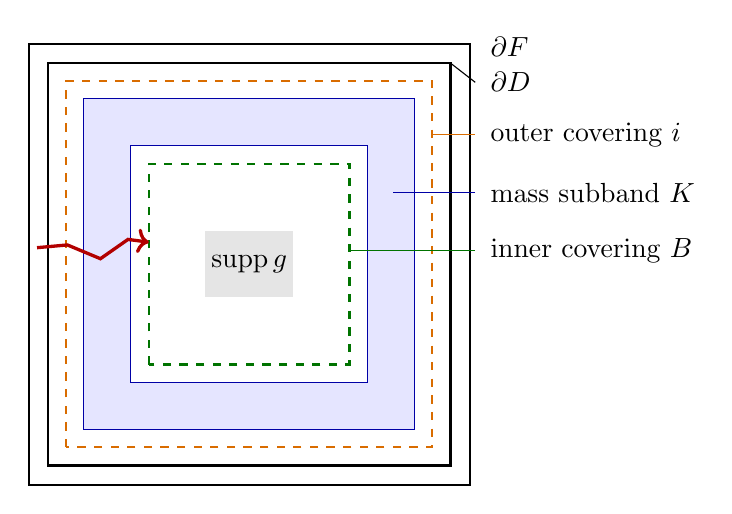
\begin{tikzpicture}[scale=.70]
 \fill[blue!10,even odd rule] (-3,-3) rectangle (3,3)
                           (-2.15,-2.15) rectangle (2.15,2.15);
 \draw[thick] (-4,-4) rectangle (4,4);
 \draw[thick] (-3.65,-3.65) rectangle (3.65,3.65);
 \draw[blue!65!black] (-3,-3) rectangle (3,3);
 \draw[blue!65!black] (-2.15,-2.15) rectangle (2.15,2.15);
 \draw[dashed,orange!85!black,thick] (-3.32,-3.32) rectangle (3.32,3.32);
 \draw[dashed,green!45!black,thick] (-1.82,-1.82) rectangle (1.82,1.82);
 \fill[gray!20] (-.8,-.6) rectangle (.8,.6);
 \node at (0,0) {$\supp g$};
 \node[anchor=west] at (4.2,3.95) {$\partial F$};
 \node[anchor=west] at (4.2,3.30) {$\partial D$};
 \draw (4.1,3.30)--(3.65,3.65);
 \node[anchor=west] at (4.2,2.35) {outer covering $i$};
 \draw[orange!85!black] (4.1,2.35)--(3.32,2.35);
 \node[anchor=west] at (4.2,1.30) {mass subband $K$};
 \draw[blue!65!black] (4.1,1.30)--(2.60,1.30);
 \node[anchor=west] at (4.2,.25) {inner covering $B$};
 \draw[green!45!black] (4.1,.25)--(1.82,.25);
 \draw[->,very thick,red!70!black]
       (-3.85,.3)--(-3.30,.35)--(-2.7,.1)--(-2.2,.45)--(-1.82,.4);
\end{tikzpicture}
\caption{The annular comparison, schematically.  The coverings
are finite unions of small cells around the dashed rings.  They
have positive clearance from the mass subband, the test support,
and $\partial D$.  An exploration reaching the test support from
$F\setminus D$ must pass both coverings.  The drawing does not
restrict the finite-range paths to nearest-neighbor paths.}
\label{an:band-figure}
\end{figure}

\begin{proposition}[Vanishing reach]\label{an:reach}
Suppose $a>0$.  Under the band law, explore all components meeting $F_n\setminus
D_n$.  The probability that any visited vertex is in a fixed
neighborhood of $\supp g$ tends to zero in
\eqref{an:limit-order}.  The same conclusion holds for an
exploration starting from a fixed positive-area region on one
side of a separating positive-width band and reaching a fixed
closed region on its other side, provided the closure of the starting
region and the target have fixed positive clearance from the band.
The two gaps admit the mass-free covering families used below, with
all clearances fixed before the lattice and band limits.
\end{proposition}

\begin{proof}
Choose finite coverings by small observation squares $B$ of an
inner ring and by squares $i$ of an outer ring, leaving the
clearances shown in Figure~\ref{an:band-figure}.  Use slightly
overlapping enlarged squares so every path crossing the rings
hits the coverings also after lattice rounding.  The maximum
scaled jump tends to zero, so a path from the starting set to the
target must meet both coverings, in order.

Let $C_0$ be the uniform bare variance bound for the remaining
average in a cell reached by a path from afar, from
Lemma~\ref{an:path-poincare}.  The cell radii can be chosen so
small that their continuum prior variances under $T_\lambda^{-1}$
are at least $C_0+2c_0$ for some $c_0>0$, uniformly over
$\lambda>0$.  To see this directly, center a truncated logarithm
at the cell and cut it off inside a fixed surrounding ball
disjoint from the mass.  Its mean over a radius-$\delta$ cell is
$c\log(1/\delta)+O(1)$, while its gradient energy is
$c'\log(1/\delta)+O(1)$.  The inverse variational principle
therefore makes the cell-average variance grow at least as
$c''a\log(1/\delta)$.  This trial pays no mass term.  Fix the
coverings at this point.  Lemma~\ref{an:band-density} gives the
same strict deficit $c_0$ for fine $\ell,n$ at each fixed
$\lambda$.

Write the average at $B$ after exterior exploration as
$h_B=e_B+u_B$, its exposed and unexposed contributions.  On
omitting the linear tilt, the conditional form is obtained from
the prior form by zero-pinning visited vertices and tightening
the cable remainders.  The partial average $u_B$ is precisely
the original full test after those zero pins.  Thus its centered
variance $w_B$ is at most the full prior variance $v_B$ by
Lemma~\ref{st:finite-gaussian}, and on a visit to $B$ it is at
most $v_B-c_0$ by the local bound.  Equations
\eqref{an:tilt-bounds} and \eqref{an:tilt-moments} show that
restoring the tilt changes the conditional second moment, and
the cross term with $e_B$, by $o(1)$ after averaging.  The needed
moments of $e_B$ follow from Lemma~\ref{an:weighted-moments}.
The prior identity $\E h_B^2=v_B$ consequently implies
\[
 c_0\Prob_W(B\text{ reached})\le\E_We_B^2+o(1).
\]
Every cluster contributing to $e_B$ is macroscopic, with a
threshold fixed by its distance from the starting set.  Sign
resampling, including the same signless selection of exterior
clusters, converts its second moment to the squared-mass sum:
\begin{equation}
 c_0\Prob_W(B\text{ reached})
 \le\E_W\sum_{C\text{ meeting the starting set}}M_C(B)^2+o(1).
 \label{an:exterior-deficit}
\end{equation}

A second deficit bounds this right side.  For each $x\in B$
with $\E_W|h_x|>0$, bias the prior by $|h_x|$ and explore only
the cluster of $x$.  Its pre-exploration variance for $h_i$ is
at least $v_i$ by \eqref{an:size-bias}.  The bias is measurable
at completed exploration and hence cancels from the conditional
law of the complement.  Its centered remaining variance is at
most $v_i$, and is at most $v_i-c_0$ if the cluster visits $i$.
Its exposed average has absolute value $M_{C(x)}(i)$.
Apply total second moment in this biased law, multiply by
$\E_W|h_x|$ and the averaging weight of $x$ in $B$, and sum in
$x$.  The terms without a visit or a tilt cancel in the
comparison with $v_i$.  Clusters causing a tilt must reach the
mass cells, and clusters contributing at $i$ must reach $i$;
both are macroscopic because all three regions have positive
separation.  Their remaining errors are bounded by a constant
times the expectation in \eqref{an:summed-tilt}, which tends
to zero.  A point with $\E_W|h_x|=0$ contributes zero directly.
The result is the exact weighted deficit
\begin{equation}
 c_0\E_W\sum_{C:C\cap i\ne\varnothing}M_C(B)
       \le\E_W\sum_CM_C(B)M_C(i)^2+o(1).
 \label{an:biased-deficit}
\end{equation}
In particular no estimate on an unsigned sum over all
microscopic clusters has been used.

The inverse forms $T_\lambda^{-1}$ decrease as
$\lambda\to\infty$ to the form inverse with every function
zero almost everywhere on $K$.  Indeed bounded energies give
weak $H^1$ compactness and $\int_Kv^2\to0$; the variational
principle gives both the limit and recovery by functions already
zero there.  This hard band separates the inner and outer
regions, so its inverse has zero cross quadratic form for
smears on opposite sides.  Equation~\eqref{an:cross-cluster}
therefore makes $\E\sum_CM_C(B)M_C(i)$ tend to zero after
\eqref{an:limit-order}.  Truncate first at
$\max_CM_C(i)\le M$.  On this event the right side of
\eqref{an:biased-deficit} is at most $M$ times this vanishing
cross sum.  Its tail tends to zero uniformly as $M\to\infty$:
\[
 \sum_CM_C(B)M_C(i)^2\le\sqrt{Q_B}\,Q_i,
\]
and Lemma~\ref{an:resampling} gives arbitrarily high uniform
moments after the first two limits.  Thus
$\E\sum_{C\cap i\ne\varnothing}M_C(B)\to0$.

Every exterior-connected cluster meeting $B$ must visit some
outer covering cell $i$.  On $\max_CM_C(B)\le M$ its
contribution to \eqref{an:exterior-deficit} is at most $M$ times
the sum of the just estimated first-mass quantities.  The
remaining tail is again controlled by the uniform moments of
$Q_B$.  Send $M\to\infty$ after the three limits.  Each $B$ is
reached with probability tending to zero, and their finite
cover gives the assertion.  The proof for a different starting
region only replaces the filled exterior by that region; the
path anchoring and the two separated coverings have exactly the
same hypotheses.
\end{proof}

\begin{theorem}[Dirichlet and torus transfer]\label{an:dirichlet-torus}
For $a(k)>0$, the centered, unprojected zero-Dirichlet height law
on every fixed square converges, in smooth density observations
and their Laplace transforms, to the real zero-Dirichlet GFF of
covariance $a(k)(-\Delta_D)^{-1}$.  For growing square tori, at
every $k>0$ the mean-subtracted height field converges to the
mean-zero torus GFF with covariance $a(k)(-\Delta_{\T^2})^{-1}$,
where $a=0$ denotes the zero distribution.  Convergence holds
along every sequence of increasing integer side lengths and in
$H^{-3}(\T^2)$.  For smooth mean-zero $f$,
\begin{equation}
 \lim_{n\to\infty}\log\E e^{H_n(f)}
     =\frac{a(k)}2(f,(-\Delta_{\T^2})^{-1}f).
 \label{an:torus-laplace}
\end{equation}
On the positive branch the uniquely determined temperature
coefficient in Equation~\eqref{main:coefficient-convention} is
\begin{equation}
 \beff(J,\beta)=v_J^2a(\beta/v_J^2).
 \label{an:effective-temperature}
\end{equation}
\end{theorem}

\begin{proof}
Consider $X_n=(h,A_0g_n)$ in the free square with the band.
On the success event of Proposition~\ref{an:reach}, the exposed
contribution to $X_n$ is zero.  Its centered conditional
variance is at most its massless zero-Dirichlet variance in
$D_n$: the centered posterior has zeros on the whole exterior,
possibly further pins and tightened edges, and the remaining
positive band precision.  Drop the latter extra conditions
using Lemma~\ref{st:finite-gaussian}.  The linear-tilt error
vanishes by \eqref{an:tilt-bounds} and
\eqref{an:tilt-moments}.  On failure, Cauchy--Schwarz bounds
$\E_W[X_n^2\ind_{\mathrm{failure}}]$ by its fourth-moment
root times the square root of the failure probability.
Lemma~\ref{an:band-density} bounds this fourth moment uniformly
after the first two limits and toward the last limit.  Hence
\eqref{an:band-saturation} implies
\begin{equation}
 \liminf_{n\to\infty}\Var_D(h,A_0g_n)
      \ge a\int_D|\nabla g|^2.
 \label{an:dirichlet-lower}
\end{equation}
This is valid along every subsequence of lattice sizes: one
uses that subsequence in the band argument before the other
limits.  Free-square cutting gives the opposite bound, with
the same gradient energy, for the zero-Dirichlet law.  Its
logarithmic moment generating function has the covariance
quadratic lower bound of Lemma~\ref{st:finite-gaussian}.
The matching upper bound follows by cutting into cells of
relative side $r$, Taylor-expanding their centered
subGaussian logarithmic moment generating functions to second
order, and summing the $O(r^3)$ remainder over $O(r^{-2})$
cells, as in Theorem~\ref{st:free-rectangle-limit}.  Discarded
edge flows have vanishing bare cost before cutting.  Thus it
has the asserted Gaussian limit for compactly supported shifts.

To pass to density tests, use the deterministic inverse-form
liminf and recovery argument given later in the proof of
Lemma~\ref{an:forms}, with the zero condition imposed on every
face of this square.  That part of the proof uses only
nearest-neighbor compactness, finite differences, and smooth
recovery; it does not use the height transfer proved here.
For the area-weighted samples $f_n$ of a smooth density, let
$A_{0,D_n}$ denote the zero-exterior Dirichlet operator.  Its inverse
quadratic form therefore converges to
$(f,(-\Delta_D)^{-1}f)$.  Put $v=(-\Delta_D)^{-1}f$ and choose
$g_j\in C_c^\infty(D)$ converging to $v$ in $H_0^1(D)$.  The
inverse variational identity gives, at each fixed $j$,
\[
 \lim_{n\to\infty}
 (f_n-A_{0,D_n}g_{j,n},
 A_{0,D_n}^{-1}(f_n-A_{0,D_n}g_{j,n}))
 =\int_D|\nabla(v-g_j)|^2.
\]
Here the cross pairing and the sampled shift energy converge by
finite differences; the inverse term is the deterministic limit
just cited.  Letting $j\to\infty$ makes the bare error vanish,
so Gaussian domination transfers the Laplace limits.  This proves
the full density-test statement and
joint convergence by real linear combinations.  In this
argument the band constant was integrated, rather than fixed;
the resulting Dirichlet law is consequently unprojected.

For a torus shift supported in a small square chart, impose
the equalities that all heights outside that square have one
common value.  They can be imposed by diverging positive
quadratic penalties.  Modulo the additive lattice constant,
the resulting law is the zero-Dirichlet square law.  The
observable annihilates constants, so comparison gives the
same lower bound \eqref{an:dirichlet-lower}.  Free-cell
cutting gives the upper bound $a\int|\nabla g|^2$ for every
smooth torus shift.  The limiting difference between this
upper quadratic form and the actual covariance is positive
semidefinite on each finite list, on every convergent
subsequence.  A vector at which it vanishes belongs to its
null space.  Each chart-supported shift has full variance convergence by the
liminf and limsup bounds just proved. A finite partition of unity writes
an arbitrary smooth torus shift as a finite sum of such shifts.
On every covariance-convergent subsequence, all their defect diagonal
entries therefore vanish simultaneously. Positive semidefiniteness
annihilates their span, and the arbitrariness of the initial subsequence
proves full variance convergence for the sum.
For $a=0$ the upper bound alone gives saturation.  The same
small-cell upper bound and Hessian lower bound give the
Gaussian Laplace limit for these shifts.

Given mean-zero $f$, solve $-\Delta g=f$ on the torus with
zero mean.  On samples, $A_0g_n$ differs from the
area-weighted sample $n^{-2}f_n$, with its sampled mean
subtracted, by a density error tending to zero in scaled
$L^2$.  This follows from the quadratic symbol of $A_0$ and
smooth finite differences.  The discrete Poincar\'e Inequality
and bare domination control the error in every exponential
moment with a fixed argument.  This proves
\eqref{an:torus-laplace} and all joint smooth projections.

Finally consider the Fourier coefficient at $m\in\Z^2$ of
$H_n$.  If $m$ is zero modulo $n$, mean subtraction makes
the coefficient zero.  Otherwise replace $m$ by its
representative $\tilde m$ with coordinates of magnitude at
most $n/2$.  The nearest-neighbor lower bound on the symbol
gives its bare second moment at most
$Ck/|\tilde m|^2\le Ck$, uniformly in $n,m$.
Consequently
\[
 \sup_n\E\|H_n\|_{H^{-2}(\T^2)}^2
       \le Ck\sum_{m\in\Z^2}(1+|m|^2)^{-2}<\infty.
\]
Compact embedding into $H^{-3}$ gives tightness; the smooth
joint projections identify every limit and hence the full
sequence.  A nonzero smooth test identifies $a$ uniquely.
Restoring the normalization in Equation~\eqref{main:coefficient-convention} proves
\eqref{an:effective-temperature}.
\end{proof}

\begin{corollary}[The physical roughness criterion]\label{an:physical-criterion}
For every fixed $J$ and $k>0$,
\begin{equation}
 a(k)>0\quad\Longleftrightarrow\quad
 \sup_{R\ge1}\E_{\mu^0_{J,v_J^2k,R}}h_0^2=\infty.
 \label{an:physical-equivalence}
\end{equation}
\end{corollary}

\begin{proof}
When $a=0$, Proposition~\ref{st:zero-localization} gives the
uniform zero-boundary point-variance bound.  Conversely suppose
the supremum on the right were finite, say at most $C_0$.
For any vertex $x$ of any zero-boundary square, translate that
square by $-x$ and enlarge to a centered square.  Relaxing
the additional zero pins increases variance, so
$\E h_x^2\le C_0$.  Cauchy--Schwarz then gives
$\Var(h,f)\le C_0(\sum_x|f_x|)^2$ for every smear.

Choose a compactly supported logarithmic pole in an interior
disk, smoothed at radius $\delta$.  More explicitly, let it
equal $\log(1/|z|)$ on $2\delta\le|z|\le r_0$, smooth it
radially to a constant at $|z|\le\delta$, and multiply by a
fixed cutoff supported strictly inside the square.  Its
gradient energy grows as $2\pi\log(1/\delta)+O(1)$, while
$\int|\Delta g_\delta|$ stays bounded: the inner radial
Laplacian has bounded total mass, and the outer cutoff is
fixed.  At each fixed $\delta$, finite differences give a
uniform bound on $\sum_x|(A_0g_{\delta,n})_x|$ as
$n\to\infty$.  Equation~\eqref{an:dirichlet-lower} would
therefore bound $a\int|\nabla g_\delta|^2$ by a constant
independent of $\delta$.  This is impossible if $a>0$.
\end{proof}

\begin{proposition}[Order and one-sided regularity of the coefficient]
\label{an:coefficient-regularity}
The function $a:(0,\infty)\to[0,\infty)$ is nondecreasing,
upper semicontinuous, and bounded above by $k$.  It is strictly
increasing on its positive set.  More precisely, if $k_2>k_1$
and $a(k_1)>0$, then
\begin{equation}
 \frac1{a(k_2)}\le\frac1{a(k_1)}+
                                    \frac1{k_2}-\frac1{k_1}.
 \label{an:strict-growth}
\end{equation}
If its positive set is nonempty, it equals $[k_c,\infty)$
for some $k_c\ge8\pi$, and the physical critical temperature
is $\bc(J)=v_J^2k_c$.  In particular the endpoint is rough.
\end{proposition}

\begin{proof}
Finite precision comparison proves monotonicity and the bare
bound $a\le k$.  The affine cutting estimate used to define
$a$ gives, for each fixed cell size $m$,
\[
 \sqrt{a(k)}\le\sqrt{a_m(k)}+C\sqrt{k/m},
\]
with harmless vanishing normalization errors if the finite
affine energy is not exactly one.  The constants are uniform
for $k$ in compact subintervals of $(0,\infty)$.
Each finite-cell quantity is continuous in $k$, by absolute
Gaussian summation, and $a_m(k)\to a(k)$.  Taking the
upper limit as $k'\to k$ and then $m\to\infty$ proves upper
semicontinuity.

For strict growth let $A_b$ be a free-cell Laplacian and let
$g$ be a nonconstant affine shift.  Work modulo constants,
put $X=(h,A_bg)$, $E_g=(g,A_bg)$, and
$U(k)=\Var X/E_g>0$.  Differentiation of its finite Gaussian
sum gives
\[
 U'(k)=\frac{\Cov(X^2,(h,A_bh))}{2k^2E_g}.
\]
Diagonalize the positive form $A_b$ on the mean-free space.
The paired fourth-cumulant positivity of
Lemma~\ref{st:finite-gaussian} bounds the numerator below
by $2(q,A_bq)$, where $q=\Cov(h,X)$.
Since $(q,A_bg)=\Var X$, Cauchy--Schwarz in the
$A_b$-energy gives $(q,A_bq)\ge(\Var X)^2/E_g$.
Thus $U'\ge U^2/k^2$.  Integrating the derivative of $1/U$
and passing to growing affine cells proves
\eqref{an:strict-growth}.  Its right side is positive since
$a(k_1)\le k_1$, and is strictly smaller than $1/a(k_1)$,
proving strict increase.

The gap in Corollary~\ref{st:charge-gap} is
$a\in\{0\}\cup[8\pi,\infty)$.  Monotonicity makes a
nonempty positive set an upper interval.  At its infimum,
upper semicontinuity and the gap force a positive value;
$a\le k$ implies $k_c\ge8\pi$.
Corollary~\ref{an:physical-criterion} identifies this same
infimum with the stated physical criterion and includes its
endpoint.  Nonemptiness and the exact endpoint value,
differentiability above it, and the infinite endpoint slope
are established in the later weak-height and endpoint
arguments; none of those conclusions is assumed here.
\end{proof}

\subsection{Fixed mixed domains and the high law}

We now fix $k_h$ with $a_h=a(k_h)>0$.  The results in this
subsection are at this one input temperature; they assert no
uniform scaling theorem at nearby temperatures.  Lengths are
measured in observation-cell units.  On the lattice an
observation cell has side $s$, with $s\to\infty$ along dyadic
integers, and $B_s$ takes its uniform height average.  A fixed
continuum cell has side one, and $B$ takes its integral average.

\begin{definition}[Permitted mixed geometry]\label{an:geometry}
Start with axis-parallel squares of a fixed dyadic side $R$.
Remove from each corner the part of the square of side $R/2$
centered at that grid vertex, and declare the latter squares
to be separate tiles.  Thus no tile vertex involves more than
three tiles, and every pair of tiles meeting there also shares
a nondegenerate face.  Take finite unions of these tiles,
possibly clipped along the $R/4$ grid by boxes.  Tiles may be
isolated by removing every bond between them and other tiles.
All exterior boundaries are free.  Components are formed by
face connections; boundary point contacts do not join them.
Round all faces on observation-cell boundaries and retain only
the prescribed internal $J$-bonds.  Each component before hard
pinning is a bounded Lipschitz union of squares with no
opposite-only junction.  Hard pins are finite unions of tiles
or boxes on the indicated subdivision grid.  The energy space
is always that of the component before pinning, with functions
zero almost everywhere on the pinned boxes.
\end{definition}

Figure~\ref{an:mixed-geometry-figure} shows the tile partition and its
three-tile junctions.

\begin{figure}[tb]
\centering
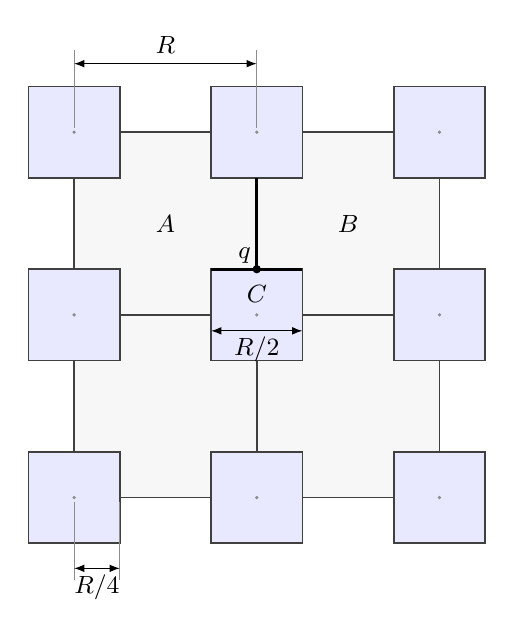
\begin{tikzpicture}[x=.58cm,y=.58cm,font=\small,
  tile/.style={draw=black!75,line width=.55pt,line join=miter},
  measure/.style={thin,{Latex[length=1.3mm]}-{Latex[length=1.3mm]}}]
  \foreach \a in {0,4}{\foreach \b in {0,4}{
    \begin{scope}[shift={(\a,\b)}]
      \path[tile,fill=black!3]
        (1,0)--(3,0)--(3,1)--(4,1)--(4,3)--(3,3)
        --(3,4)--(1,4)--(1,3)--(0,3)--(0,1)--(1,1)--cycle;
    \end{scope}
  }}
  \foreach \a in {0,4,8}{\foreach \b in {0,4,8}{
    \path[tile,fill=blue!9] (\a-1,\b-1) rectangle (\a+1,\b+1);
    \fill[black!45] (\a,\b) circle (.65pt);
  }}
  \draw[line width=1.05pt] (3,5)--(5,5) (4,5)--(4,7);
  \fill (4,5) circle (1.5pt);
  \node[anchor=south east,inner sep=2pt] at (4,5) {$q$};
  \node at (2,6) {$A$};
  \node at (6,6) {$B$};
  \node at (4,4.45) {$C$};
  \draw[black!45,thin] (0,8.1)--(0,9.8) (4,8.1)--(4,9.8);
  \draw[measure] (0,9.5)--node[above] {$R$} (4,9.5);
  \draw[measure] (3,3.65)--node[below,inner sep=2pt] {$R/2$} (5,3.65);
  \draw[black!45,thin] (0,-.1)--(0,-1.8) (1,-.1)--(1,-1.8);
  \draw[measure] (0,-1.55)--node[below,inner sep=2pt] {$R/4$} (1,-1.55);
\end{tikzpicture}
\caption{Permitted mixed tiles in Definition~\ref{an:geometry}.  Each original $R$-square loses its four
$R/4$-square corners to distinct $R/2$-squares centered at the original
grid vertices (dots); four trimmed originals and their vertex tiles
are shown.  The $R/4$ tick marks the subdivision scale.  At $q$, the
three incident tiles $A,B,C$ share the three bold boundary segments pairwise;
only two tiles meet at a corner of $C$.
Later components are formed by retained face/bond connections;
point contacts alone do not join components.}
\label{an:mixed-geometry-figure}
\end{figure}

The proofs also apply to any fixed finite list of domains with
these geometric properties, including the rectangular strips
used below.  In particular, touching boundary points never
glue two components through a set of zero continuum capacity.
For the deterministic form arguments this includes fixed finite
face-connected unions of rectangular pieces with bounded lattice
rounding, provided retained faces have the local bounded routes
used below and neither point-only nor opposite-only contacts glue
components.

On a fixed such open graph $U_s$, let $A_{0,U_s}$ retain just
its prescribed bonds.  For real observation values $y$ put
\begin{align}
 Z_U(y;k)&=\sum_{h\in(2\pi\Z)^{U_s}}
  \exp\left\{-\frac{(h,A_{0,U_s}h)}{2k}
                    -\frac12\|B_sh-y\|^2\right\},
 \label{an:high-partition}\\
 E_U(y;a')&=\min_v\left\{
       \frac{(v,A_{0,U_s}v)}{a'}+\|B_sv-y\|^2\right\}.
 \label{an:comparison-energy}
\end{align}
An indicated hard pin imposes $h=0$, or $v=0$, throughout
the specified set.  Translation sums are included in
\eqref{an:high-partition}; the observation mass controls
every component's constant mode.  Write $P_U$ for the
centered high law $y=0,k=k_h$.  In the continuum, the
comparison high precision at $a'=a_h$ is the coercive form
\begin{equation}
 \mathcal T_U(v,w)=a_h^{-1}\int_U\nabla v\cdot\nabla w
                             +\sum_{d\subset U}(Bv)_d(Bw)_d
 \quad\text{on }H^1(U).
 \label{an:continuum-high-form}
\end{equation}
Impose the specified zero conditions when pins are present.
Superscript $\mathrm{cg}$ denotes this continuum Gaussian
comparison.  Without pins, $E_U$ annihilates constants on
each component.

\begin{lemma}[Form and free-component limits]\label{an:forms}
On every fixed geometry of Definition~\ref{an:geometry},
the discrete real-Gaussian forms converge to their continuum
forms, with their stated free and zero-region boundary
conditions.  Inverse quadratic forms converge for bounded
piecewise continuous density tests on coercive components.  On a
massless free component the test must have zero total, separately
on every released component.  Energy approximation is valid for
shifts and trace-preserving combinations.
The massless free height law at $k_h$, modulo its constant,
has covariance $a_h$ times the Neumann inverse form and
Gaussian Laplace limits on every component.  Its fractional
mean is uniform modulo $2\pi$, independently of any fixed
list of mean-free observations.
\end{lemma}

\begin{proof}
For smooth functions on a neighborhood of the closure,
the discrete energies converge to $\int|\nabla v|^2$:
the symbol of $A_0$ has quadratic part $|p|^2$, internal
Riemann sums converge, and the number of edges within a
fixed lattice distance of the finitely many faces and
corners is $O(s)$, each with squared smooth difference
$O(s^{-2})$.  Nearest-neighbor edges control the
$H^1$ norm of piecewise affine interpolants on each
constituent square, modulo a componentwise constant.
Conversely all fixed-range differences are bounded by a
fixed multiple of nearest-neighbor energy on local
face-connected patches: a retained jump can be replaced
by a nearest-neighbor route of bounded lattice length
in one of the finitely many local square-sector patterns.
There are no opposite-only contacts.  Thus bounded
energies give weak $H^1$ compactness on the squares,
strong $L^2$ compactness, and matching traces across
retained faces.  The difference quotients for each
step pass weakly to their directional derivatives.
Their sum and the lattice symmetries give the
continuum liminf energy with its exact coefficient.

Here is the density statement with pins and corners.
First truncate an $H^1$ function to bounded magnitude;
this decreases gradient energy and preserves every
zero region.  Around each polygon vertex use a cutoff
which is zero within radius $\delta^2$, one outside
radius $\delta$, and linear in $\log r$ between.
Its squared gradient integral is $O(1/|\log\delta|)$.
For a bounded function this removes all vertices at
vanishing energy and $L^2$ cost.  Away from them, a
pinned straight face is treated by the zero-trace
$H^1$ approximation on a half-rectangle, extending by
zero into the pin before mollification.  On a free
face use even local extension and mollification.
Interior patches are mollified directly.  A finite
partition of unity combines these approximations.
They show that restrictions of smooth ambient
functions are dense without pins, and functions
smooth away from vertices and vanishing in a
neighborhood of the pinned region are dense with
pins.  Sampling these functions gives recovery
sequences.  Observation-cell averages are continuous
under strong $L^2$ convergence.  The same liminf and recovery
proof applies to a square with zero trace on every face, using
zero extension on each face; this is the deterministic
$H_0^1$ inverse-form assertion used in
Theorem~\ref{an:dirichlet-torus}.  Neumann Poincar\'e
and cell masses, or a fixed positive-area hard pin,
control constants.  Minimizing the coercive forms
minus a linear density source now proves inverse
convergence by the liminf and recovery statements.
The same reasoning, modulo constants, treats zero-total
densities in an unpinned component.

For the height law, enclose the component in a larger
free square.  For a smooth ambient shift, separate
its gradient observation into the retained pieces
on the component and on the finitely many remaining
polygonal pieces.  The omitted seam flows have
vanishing bare squared cost by their $O(s)$ number
and $O(s^{-1})$ coefficients.  Cutting increases
covariances; the resulting independent component
variances each have the continuum gradient upper
bound, by further subdivision into squares.
Their sum already attains that bound in the
enclosing free square by
Theorem~\ref{st:free-rectangle-limit}.
Write $U_i$ for the retained pieces and $V_{i,s}$ for their
partial gradient-observation variances.
For each component $i$, subtract the limsup upper bounds for the
other finitely many pieces from the full limiting enclosing-square
variance. The cutting inequality gives
$\liminf_sV_{i,s}\ge a_h\int_{U_i}|\nabla g|^2$.
Together with its upper bound this proves full variance convergence on
that component, along every admissible mesh sequence.
The density of ambient shifts just proved and bare error bounds give
full variance convergence on its full $H^1$ energy space.  Cutting into small
cells and the second-order logarithmic moment
expansion used in Theorem~\ref{an:dirichlet-torus}
give the Gaussian Laplace limits.  The form
approximation transfers them to the stated density
observations.

Finally consider a character with nonzero integer
total charge on one component, including fixed
mean-free observations if desired.  Extend its
source by zero to the enclosing square.  The
dual shifted-ratio precision comparison from
Lemma~\ref{st:finite-gaussian} bounds its positive
characteristic function in the cut component by
that in the uncut square.  This can first be done
with a tiny positive mass, then passed to the
translation-modulo law because its total is an
integer.  Approximation by bounded-density profiles
is justified by the bare norm bounds.  The enclosing
character tends to zero by
Theorem~\ref{st:fractional-mean}.  The same argument
with joint mean-free sources, or Fourier
approximation of a bounded function of those
sources, proves independence of the uniform
fractional mean.  Distinct free components were
independent from the outset.
\end{proof}

For finite observation penalties below, fix a finite vector
$\mathcal O_s h$ of cell averages or bounded piecewise continuous
density smears covered by the preceding joint limits, with uniformly
bounded bare covariance after constants are removed.  An admitted
quadratic penalty is
\[
 \exp\{-\tfrac12(\mathcal O_s h-z)^TQ(\mathcal O_s h-z)\},
 \qquad Q\ge0.
\]
The observation family is fixed through the mesh limit.  Its center
and coefficient matrix may range over a fixed compact set.  Each
observation lies in one pre-pin component, and $Q$ has no entries
coupling different components.  If a
component constant is free, the induced quadratic form on the vector
of released constants must have a common positive lower bound.
Thus every such penalty confines all released constants.

\begin{proposition}[Mixed-boundary height scaling]\label{an:mixed-scaling}
On a fixed permitted component meeting a nonempty
positive-area pin region, the centered massless height
law at $k_h$ has the full Gaussian Laplace and moment
limits with covariance $a_h$ times the mixed inverse:
zero on that entire region and free on the other
walls.  This includes bounded piecewise continuous
smears and energy-approximable shifts.  Adding an admitted finite
observation penalty gives the corresponding Gaussian limit, also
for components without hard pins when translations are summed.
The limits are uniform over the fixed compact coefficient and center
sets just specified.
\end{proposition}

\begin{proof}
It suffices first to use a smooth shift $g$ vanishing
on a neighborhood of the pin $p$, but allowed to
reach the outer free walls.  Choose a subband of
positive width between $p$ and $\supp g$, separated
by positive gaps from both.  It may follow level
strips of sup distance to the whole pin region,
clipped to the component.  Select levels on a
sufficiently fine fixed rectangular grid, then
subdivide into mass cells.  All clearances are
fixed before the fine lattice limit.  Where the
pin has several components, use the union of
these strips and retain those connected pieces
through which a path to the support is possible.

Start with the component unpinned, put the band
weight on it, and explore from the entire pin
region.  Lemma~\ref{an:forms} supplies the free
Gaussian and fractional-mean inputs to
Lemma~\ref{an:band-density}.  Its Hilbert--Schmidt
bound follows by cutting the domain into finitely
many squares: their $H^1$-to-$L^2$ inclusions have
fourth-power summable singular values, which
bounds the square of the Neumann inverse after
the component constant is removed.  The band
controls that constant as before.

We verify the local hypotheses of the exploration
lemmas at free walls and junctions.  A fixed-factor
enlargement of a touched small cell within the
component is a connected patch of a bounded number
of comparable rectangles, joined by straight
faces of comparable length.  Its Poincar\'e
constant is $C\ell^2$: apply the rectangle
inequalities and bound the differences of their
means across the common faces by the same
gradient energy.  Truncate a visiting path when
it spans a comparable cell distance.  Some
coordinate then spans $c\ell s$ levels.  Bounded
jumps and the bounded number of local rectangles
put a positive fraction of anchored rows or
columns into one of these rectangles.  The
one-dimensional estimate in
Lemma~\ref{an:path-poincare} anchors its mean;
the patch Poincar\'e Inequality anchors the
remaining rectangles.  At a corner use all
adjacent sectors of the same component.  The
no-opposite-only convention ensures that a
retained jump lies in a sector or crosses between
sectors joined through retained faces.  A filled
starting pin region itself supplies the initial
zero extension for variations.  Thus the same
local inequality \eqref{an:local-path-bound}
holds, and a fixed macroscopic path anchors the
whole component.  Small-cell mean-free bare
variance still costs $C(1+\log(1/\ell))$:
compare first to a containing fixed square patch
using its Neumann modes, and then use the
component Poincar\'e Inequality to compare means.

The two coverings can be made of subdivisions
reaching the free walls.  A logarithmic trial
restricted from the plane to a straight or
sector patch has cell average and gradient
energy proportional to $\log(1/\delta)$, with
positive geometric constants; it therefore
gives the large pre-exposure variance required
in Proposition~\ref{an:reach}.  The anchored
post-exposure bound is independent of the cell
radius.  For the size-bias step take the
starting covering on the test side, with the
other covering on the pin side; both are away
from the mass.  Every nonzero tilt or exposed
contribution between them again requires a
macroscopic cluster.  All of
Lemmas~\ref{an:reinsertion}--\ref{an:tilt} and
both deficits \eqref{an:exterior-deficit},
\eqref{an:biased-deficit} therefore apply with
the same limit order.  The hard-band inverse
separates the sides, so reach of the support
has vanishing probability.

The weak Laplacian source of $g$ is the energy functional
$F_g(v)=\int_U\nabla g\cdot\nabla v$, including its free-face
contributions.  Its discrete observation
$X_s=(h,A_{0,U_s}g_s)$ is translation invariant and has bounded
bare variance
\[
 \Var_{\rm bare}X_s
 \le k_h(g_s,A_{0,U_s}g_s)=O(1).
\]
At each fixed band partition and strength, include $X_s$ in the
joint free-component limit from Lemma~\ref{an:forms}.  The
translation-sum bound in the proof of Lemma~\ref{an:band-density}
and this bare bound give uniform integrability of every fixed
power of $X_s$ under the normalized band law.  Since every mass-cell
average of $g$ is zero, the continuum projected band form on $U$,
\[
 \mathcal T_{\ell,\lambda}(v,w)
 =a_h^{-1}\int_U\nabla v\cdot\nabla w
       +\lambda\sum_d|d|v_dw_d ,
\]
satisfies
\[
 \mathcal T_{\ell,\lambda}(a_hg,v)=F_g(v).
\]
Consequently, at every fixed $\ell,\lambda$,
\[
 \lim_{s\to\infty}\E_W X_s^2=a_h\int_U|\nabla g|^2,\qquad
 \lim_{s\to\infty}\E_W X_s^4
       =3\left(a_h\int_U|\nabla g|^2\right)^2 .
\]
The fourth-moment limit is independent of $\ell,\lambda$.
On successful exploration the centered posterior has at least
the desired pin, so its variance is at most the massless mixed
variance.  Equation~\eqref{an:tilt-moments} controls the tilt
errors.  On failure, Cauchy--Schwarz bounds the second moment by
$(\E_WX_s^4)^{1/2}\Prob_W(\mathrm{failure})^{1/2}$.
The displayed fourth-moment limit and vanishing reach make this
term vanish in the prescribed order, with no finite-mesh
uniformity in $\lambda$ required.
Run this comparison on any lattice subsequence and then take the stated
band limits. It gives the liminf lower bound
$a_h\int|\nabla g|^2$ for the actual hard-pin variance.
Free cutting gives the matching limsup, hence full variance convergence.
Free cutting also gives the upper logarithmic moment bound, and
minimal Hessian gives the matching lower
logarithmic moment bound.  The pinned density
and form approximation of
Lemma~\ref{an:forms} extends these conclusions
to the asserted tests.

An admitted finite observation penalty can now be integrated
against these joint massless limits.  In a pinned component bare
Gaussian bounds give uniform integrability for polynomial and
fixed exponential insertions.  In free components use the
independent uniform fractional means and their translation sums.
The common lower bound on the quadratic form of the released
constants gives a uniform finite-dimensional Gaussian theta bound
on these sums, as in Lemma~\ref{an:band-density}.  On a fixed compact
coefficient and center set the limiting normalizers are continuous
and bounded away from zero.  The same tail bounds give
equicontinuity of the integrals there.  This proves the last
assertion and its stated compact-set uniformity.
\end{proof}

\subsection{Separated Gaussian pins and localization}

For disjoint positive-area box regions $H,p\subset U$ at
strictly positive separation, define under the unpinned
centered high law
\begin{equation}
 D_U(H,p)=\log\frac{P_U(h_H=0\mid h_p=0)}{P_U(h_H=0)}.
 \label{an:pin-interaction-definition}
\end{equation}
An empty contribution in a component is zero.  Each hard
pin means all microscopic heights in that region vanish.
Precision monotonicity gives $D_U\ge0$, by first imposing
the pins as diverging positive quadratic penalties.  The
individual pin probabilities need not have finite or
positive continuum limits; only their interaction will
be compared.

\begin{proposition}[Gaussian pin determinant and locality]
\label{an:gaussian-localization}
All assertions in this proposition are for real Gaussians.
The discrete limits allow every integer sequence $s\to\infty$
satisfying the bounded lattice rounding and retained-route assumptions
above.  The gradient coefficient may be any fixed
$a_{\mathrm g}>0$, independently of the height input $k_h$:
for unit-cell mass replace $\mathcal T_U$ by
\[
 \mathcal T_{U,a_{\mathrm g}}(v,w)
 =a_{\mathrm g}^{-1}\int_U\nabla v\cdot\nabla w
       +\sum_{d\subset U}(Bv)_d(Bw)_d .
\]
At $a_{\mathrm g}=a_h$ this is \eqref{an:continuum-high-form}.
Let $\mathcal E_U$ be the Hilbert space with inner product
$\mathcal T_{U,a_{\mathrm g}}$.  Set
\[
 V_p=\{v\in\mathcal E_U:v=0\text{ a.e. on }p\}^{\perp},
 \qquad V_H=\{v\in\mathcal E_U:v=0\text{ a.e. on }H\}^{\perp},
\]
and denote the orthogonal projections by $\Pi_p,\Pi_H$.
Then $C=\Pi_H|_{V_p}$ is Hilbert--Schmidt and $\|C\|<1$.
The finite interaction is
\begin{equation}
 D_U^{\mathrm{cg}}(H,p)
   =-\frac12\log\det\bigl(\Id-C^*C\bigr)
   =-\frac12\log\det\bigl(\Id-\Pi_p\Pi_H\Pi_p|_{V_p}\bigr).
 \label{an:pin-determinant}
\end{equation}
The full-pin interactions for the corresponding discrete
real Gaussians converge to \eqref{an:pin-determinant} as
$s\to\infty$; for real Gaussians the interaction is the logarithm
of the corresponding density ratio at zero.

The same Hilbert--Schmidt property, norm gap, determinant formula,
full discrete pin limit, and exhaustion by finite smooth pin-density
probes hold for the modified energy space with form
\[
 a_{\mathrm g}^{-1}\int_U\nabla v\cdot\nabla w
       +(\mathcal Ov)^TQ(\mathcal Ow),\qquad Q\ge0,
\]
where $\mathcal O$ is a fixed finite family of box averages or bounded
piecewise continuous density smears, each supported in one pre-pin
component, and $Q$ has no entries coupling different components.
The fixed penalty is coercive on the whole released component-constant
subspace.  The rank, coefficients, geometry, and separated positive-area
pin regions remain fixed through the mesh limit.  This includes each
fixed confining band partition and strength.  It also applies to the
fixed face-connected rectangular-piece geometries described after
Definition~\ref{an:geometry}, with the same pre-pin energy space.

For the locality assertions below, the mass cells may also be
axis-parallel rectangles whose side lengths lie in a fixed interval
$[c_0,C_0]\subset(0,\infty)$ and whose aspect ratios are bounded.
Here $(Bv)_d=|d|^{-1}\int_d v$, $B_s$ takes the corresponding
discrete uniform averages, and every cell has the squared-average
mass with coefficient one.  These bounds include any fixed finite
normalized shape list and its bounded lattice rounding.
For this local cell mass, harmonic extension and inverse-form
sources have energy tails bounded by $Ce^{-cr}$ at
distance $r$ from their supports.  Cross-projection
Hilbert--Schmidt norms satisfy the same decay up to a
polynomial factor in the number of relevant cells, with a fixed
positive lower bound on the pin clearance for the two restrictions.
Consequently $D_U^{\mathrm{cg}}(H,p)\le Ce^{-cr}$ up to
such a factor when their separation is $r$ and their
volumes are polynomial in $r$.

For this local cell mass let $T_{U,a'}$ be the operator of
$\mathcal T_{U,a'}$ and write
$\mathsf E_{U,a'}=\Id-BT_{U,a'}^{-1}B^*$ for the matrix of
\eqref{an:comparison-energy}, with its discrete analogue
using $B_s$.  Its off-diagonal entries decay exponentially.
If bonds at a core are cut, the change of this matrix
decays exponentially as either observation index recedes
from the core.  Computing this change in an open patch
whose guard has width $r$ makes an error bounded by
\begin{equation}
 C e^{-cr-c\dist(i,j)}
 \label{an:local-energy-error}
\end{equation}
in cell entries, after local differences are extended by
zero.  All the preceding locality constants, including
the tail and cross-projection bounds, are uniform when $a'$ ranges over
a fixed compact interval in $(0,\infty)$ and on the permitted
cell ensembles with the stated uniform shape bounds and uniform
polynomial ball volumes in the cell graph.  The compared topologies use
the same $a'$.  Patch boundaries follow
cell faces and the guard width is measured in the common inclusion
cell graph.  The discrete locality estimates also hold on finite
periodic identifications satisfying the same cell and retained-route
assumptions and polynomial ball-volume bounds.  Distances are then
measured in the quotient inclusion graph, and the guard width is
the distance to the bonds actually cut to form the patch.  The patch
is a union of intact cells with all crossing bonds cut; an opened
periodic seam counts as part of its boundary.  A patch equal to the
whole component with its periodic bonds retained has zero proxy error.
Without hard pins these
change and error forms have zero row sum on each
underlying component.  Thus an entry bound with prefactor
$\delta$ and exponential distance decay bounds their
quadratic forms by
\begin{equation}
 C\delta\sum_{\{i,j\}\text{ neighboring cells in the region}}
                       (y_i-y_j)^2.
 \label{an:row-sum-gradient}
\end{equation}
For hard-wall changes one instead retains the entry
bounds on $y_i y_j$, with decay from the walls.
\end{proposition}

\begin{proof}
For the local cell form, Poincar\'e on each permitted rectangle and
the upper and lower area bounds give the uniform norm equivalence
\begin{equation}
 c\left(\|v\|_2^2+\|\nabla v\|_2^2\right)
 \le\mathcal T_U(v,v)
 \le C\left(\|v\|_2^2+\|\nabla v\|_2^2\right).
 \label{an:high-coercivity}
\end{equation}
The discrete version follows from the same cell
inequality, nearest-neighbor domination, and the
bounded routes for retained $J$-bonds.  The proof applies at any
fixed positive gradient coefficient.  More quantitatively, if
$a'\in I=[a_-,a_+]\Subset(0,\infty)$, then
\[
 \min\{1,a_h/a_+\}\mathcal T_{U,a_h}
 \le\mathcal T_{U,a'}\le
 \max\{1,a_h/a_-\}\mathcal T_{U,a_h}.
\]
Thus the coercivity, cutoff absorption, and layer-contraction
constants below can be chosen uniformly on $I$, in the continuum
and on the discrete graphs.  In the local estimates below,
$\mathcal T_U$ denotes the chosen local cell form, with its coefficient
held fixed while topologies are compared.  Each vector in
$V_p$ minimizes energy subject to its values on $p$;
it is therefore weakly harmonic for its specified form off $p$.

We give the local estimates behind compactness and
locality.  Let $v$ be harmonic away from a source
region.  Test its equation by $\chi^2v$, with a
Lipschitz cutoff supported away from the source.
Expanding the gradient term and applying
$2|ab|\le\eps a^2+\eps^{-1}b^2$ absorbs half the
gradient term and bounds the rest by the $L^2$
mass on the cutoff layer.  The average penalty in
a cell wholly inside the constant part of the
cutoff is nonnegative.  Cells meeting its
transition are contained in a bounded enlargement
of the layer, and their average cross terms are
bounded by that layer's $L^2$ mass.  Thus
\[
 \mathcal T_U(v,v;\text{inner patch})
        \le C\|v\|_{L^2(\text{enlarged patch})}^2
\]
whenever the inner patch is separated from sources
by a fixed positive margin.  Here local energy
includes entire cells, and enlarging by finitely
many cell layers absorbs the average terms.
This proof uses no integration boundary term, so
is valid up to free walls.  Discrete differences
obey the same expansion, with cutoff differences
$O(s^{-1})$ and a fixed enlargement by the
interaction range.

Using instead a cutoff which retains $v$ near its
source and removes its distant tail, harmonic
minimality and \eqref{an:high-coercivity} imply
\[
 \mathcal T_U(v,v;\dist\ge r+c_1)
     \le C\mathcal T_U(v,v;r\le\dist\le r+c_1).
\]
Equivalently each extra layer reduces the remaining
tail by a factor at most $C/(1+C)<1$.  Iteration
proves exponential energy and $L^2$ decay.  A
source in one observation cell obeys the same
bound outside that cell.  Distances may be
measured in the retained face-cell graph.  For
estimates on changing topologies they may also
be measured in the uncut inclusion-region graph:
a retained path can only become longer on
removing bonds, while a distance cutoff in the
inclusion graph still has uniformly bounded
differences on retained bonds.  Polynomial ball
volumes control the number of layer cells.
These cutoff estimates use only the local cell and route bounds
and the graph distance, so they hold on a finite periodic
identification with the quotient inclusion distance as well.

To obtain a trace estimate, cut a bounded patch
into its rectangular mass cells.  The inclusion from broken
cell $H^1$ into $L^2$ has singular values bounded
by $Cj^{-1/2}$, with the appropriate cell-count
factor, by the Neumann cosine eigenvalues on
each rectangle and the uniform side-length bounds.  The same bound
holds uniformly on discrete rectangles: the nearest-edge cosine
eigenvalues control all frequencies up to the
finite lattice cutoff.  Apply this inclusion
on a first patch, the harmonic interior bound
on a smaller patch, a second such inclusion,
and then another interior bound.  The
singular-value product inequality
$s_{2j-1}(AB)\le s_j(A)s_j(B)$ gives
\begin{equation}
 s_j(\text{restriction of harmonic extension})
          \le Cj^{-1}.
 \label{an:singular-tail}
\end{equation}
This is Hilbert--Schmidt, with uniformly vanishing
squared singular-value tails.  Leave an additional
distance margin before these two restrictions;
the exponential operator bound already proved
then multiplies the Hilbert--Schmidt bound.
Projection onto $V_H$ is unchanged when a
function is multiplied by a cutoff equal to
one near $H$, since their difference vanishes
on $H$.  The estimates therefore apply to the
cross projections.  For a fixed finite observation penalty on a
fixed domain, Poincar\'e and control of the released constants
still give coercivity with fixed constants.  If a pin gap is
smaller than a cell, or an observation crosses a cutoff patch,
retain the finitely many involved averages as extra coordinates
$F(v)\in\R^m$ in the interior estimate:
\[
 \|v\|_{H^1(\text{inner})}
 \le C\bigl(\|v\|_{L^2(\text{outer})}+|F(v)|\bigr).
\]
The same estimate holds discretely.  Each augmented inclusion
$H^1\oplus\R^m\to L^2\oplus\R^m$ has
$s_{j+m}\le Cj^{-1/2}$.  The two restrictions therefore give
$s_{2j+O(m)}\le Cj^{-1}$, which is the same square-summable
tail after a fixed index shift.  This proves compactness and
\eqref{an:singular-tail} for the modified fixed form.  Its constants
may depend on that penalty; no exponential uniformity as a band
rank or strength increases is asserted.

The intersection $V_p\cap V_H$ is zero.  In
fact choose a smooth cutoff equal to one on
$p$ and zero near $H$.  It decomposes any
$H^1$ test into a function vanishing on $p$
and a function vanishing on $H$.  A vector in
both orthogonal complements is orthogonal to
every test, hence zero.  Compactness of $C$
then gives $\|C\|<1$: equality would have an
attaining unit vector whose two projections
are both isometries, placing it in the
intersection.  For the local cell masses with the stated fixed
positive pin clearance, the cutoff can be chosen with uniformly
bounded multiplier norm
$\|\chi v\|_{\mathcal E_U}\le M\|v\|_{\mathcal E_U}$,
by the uniform local coercivity.  For a unit $v\in V_p$,
$v-\chi v$ vanishes on $p$ and $\chi v$ vanishes on $H$, so
\[
 1=\langle v,\chi v\rangle_{\mathcal E_U}
   =\langle(\Id-\Pi_H)v,\chi v\rangle_{\mathcal E_U}
   \le M\|(\Id-\Pi_H)v\|_{\mathcal E_U}.
\]
Thus $\|C\|^2\le1-M^{-2}$ uniformly.  The determinant formula
proved below and the Hilbert--Schmidt bound then give
\[
 D_U^{\mathrm{cg}}(H,p)
 \le\frac{\|C\|_{\mathrm{HS}}^2}{2(1-\|C\|^2)}
 \le\frac{M^2}{2}\|C\|_{\mathrm{HS}}^2,
\]
which supplies the uniform determinant prefactor in the local
cell estimates.  For a fixed nonlocal penalty the preceding
pointwise gap and penalty-dependent constants suffice.
For finite lists of pin
observations the Gaussian Schur formula gives
$-\frac12\log\det(\Id-C^*C)$.  Exhausting
the observation subspaces by smooth density
probes gives \eqref{an:pin-determinant}, since
$C^*C$ is trace class and has norm below one.
Densities in $p$ are total for $V_p$:
orthogonality to all their representers means
the tested energy function is zero a.e. on
$p$.  The analogous statement holds for $H$.  This totality and
Schur-formula exhaustion are in the specified energy space, so
the same argument gives the displayed determinant for every
modified fixed form in the statement.

We spell out why lattice refinement loses no
trace.  Lemma~\ref{an:forms} gives convergence
of the Gram matrices of every fixed finite
list of density representers and of their
pinned projections.  A sequence of unit-energy
discrete vectors harmonic off $p$ has weakly
convergent interpolants; testing on the dense
shifts from that lemma shows that its weak
limit is harmonic off $p$.  Conversely,
projecting a fixed representer onto $V_p$
converges strongly in energy, by convergence
of its variational minimum and norm.  If such
a bounded sequence has weak limit zero,
compact $L^2$ convergence and the interior
estimate make its energy near $H$ tend to
zero.  For a fixed observation penalty the finitely many
averages converge too, so cause no exception.
The cutoff observation just used then gives
norm convergence to zero of its projection
onto $V_H$.  It follows by contradiction
that residual cross projections outside a
growing finite probe list have uniformly
small operator norm in the lattice limit.
Equation~\eqref{an:singular-tail} makes
their Hilbert--Schmidt norms uniformly small
as well: first retain finitely many singular
directions and use the operator bound there,
then sum the uniform $j^{-2}$ tail.
Thus the cross products converge in trace
norm and are eventually bounded in norm by
a fixed number less than one.  The
Fredholm logarithm, given by
$-\log\det(\Id-K)=\sum_{m\ge1}\tr(K^m)/m$,
converges.  This proves the full discrete
Gaussian determinant limit.  The exponential
Hilbert--Schmidt estimate proves the claimed
decay of the determinant when the separation
is large; for bounded separation its fixed
geometry bound suffices.

It remains to verify the local cell statements about
$\mathsf E_{U,a'}$.  Minimizing
\eqref{an:comparison-energy} gives
$v_y=T_{U,a'}^{-1}B^*y$ and
$E_U(y;a')=y^T(\Id-BT_{U,a'}^{-1}B^*)y$.
The source-tail estimate applied to $y=e_i$
gives exponential off-diagonal entries.
Restoring bonds adds a positive form, so the
change of the minimum energy is positive
semidefinite.  If the added bonds are at a
core, use as a competitor the old minimizer
cut to zero in a neighborhood of that core.
Its energy excess over the old minimum is
exactly the squared norm of the correction
in the old form, since the old minimizer is
stationary.  The correction is supported
near the core and has energy bounded by
the tail estimate.  There is no new
cross-bond energy because it vanishes on
both ends of every restored bond.
This bounds diagonal changes by
$Ce^{-c\dist(i,\mathrm{core})}$;
positive-form Cauchy--Schwarz bounds their
entries by the geometric mean of diagonal bounds.  Let $D_{\rm full}$
and $D_{\rm patch}$ be the full and open-patch core changes, extending
the latter by zero.  If the patch retains the whole component and
all its ambient bonds, they agree.
Otherwise the core estimate bounds their difference by
$Ce^{-c(d_i+d_j)}$, where $d_i$ is the distance from index $i$ to
the core.  When both indices lie in the patch, cutting its boundary
is a direct sum because the mass is cell-local.  The same difference
is then a difference of two boundary changes and is bounded by
$Ce^{-c(b_i+b_j)}$, where $b_i$ is the distance to that boundary.
The guard gives $d_i+b_i\ge r-O(1)$, so the minimum of the two
bounds has a factor $e^{-cr}$.  If an index is outside the patch,
the patch entry is zero and that index has core distance at least
$r-O(1)$, giving the same factor from the core bound.
Independently, the full and patch energy matrices have the
off-diagonal spatial decay just proved.  Taking a geometric mean
with that bound and weakening $c$ proves
\eqref{an:local-energy-error} for every entry.  Retaining another
fraction of the core bound permits summation over cores with
polynomial cell counts.

Without hard pins a componentwise constant
$y$ has zero minimum energy; symmetry
therefore gives zero row sums for the
matrices and their differences.  A
symmetric zero-row-sum matrix $F$ obeys
\[
 y^TFy=-\frac12\sum_{i,j}F_{ij}(y_i-y_j)^2.
\]
For each pair choose a shortest
nearest-cell path in the inclusion
region.  Its length times the sum of
squared differences along it bounds
$(y_i-y_j)^2$.  Pairs of length $l$
using a given edge have both endpoints
in its $l$-ball, whose volume is
polynomial.  Summing the exponential
entry bound over $l$ proves
\eqref{an:row-sum-gradient}; no separate
flow-congestion assertion is needed.
At junctions bounded microscopic jumps
can be shadowed by face-cell paths
with bounded excess length, precisely
because opposite-only contacts are
excluded.  For hard-wall changes the
constant need not lie in the null
space, so one uses the proven magnitude
bounds directly.
\end{proof}

\begin{proposition}[Full hard-pin comparison]\label{an:pin-interaction}
For every fixed geometry and separated box regions $H,p$
as above, at $k=k_h$,
\begin{equation}
 D_U(H,p)\longrightarrow D_U^{\mathrm{cg}}(H,p)
 \qquad(s\to\infty).
 \label{an:full-pin-limit}
\end{equation}
The baseline on both sides has unit-cell observation mass,
free exterior walls, and no other hard pins.
\end{proposition}

\begin{proof}
It suffices to treat one component meeting both regions.
Place a band $K$ between them with positive clearances,
and replace the unit-cell mass by
$W_{\ell,\lambda}$.  Denote the resulting interaction
by $D_W$.  For a pin set
$Q\in\{\varnothing,H,p,H\cup p\}$, let $Z_{M,Q}$
be its partition sum with mass penalty $M$, where
$M=U$ denotes the unit-cell mass and $M=W$ the
band mass.  Direct cancellation gives the exact identity
\begin{equation}
 D_U-D_W=
 \log\frac{Z_{U,H\cup p}}{Z_{W,H\cup p}}
 +\log\frac{Z_{U,\varnothing}}{Z_{W,\varnothing}}
 -\log\frac{Z_{U,H}}{Z_{W,H}}
 -\log\frac{Z_{U,p}}{Z_{W,p}}.
 \label{an:four-mass-ratios}
\end{equation}
Each ratio is a change between two fixed finite-rank
confining penalties on the same massless domain.
For $Q\ne\varnothing$, it is the ratio of their
expectations in the normalized massless mixed law.
For $Q=\varnothing$, use the sigma-finite
per-translation-orbit normalization.  Its common
massless factor cancels inside this ratio.
Proposition~\ref{an:mixed-scaling} and
Lemma~\ref{an:forms} show that, at fixed band
partition and strength, every ratio has precisely
its Gaussian limit.  No normalization belonging
to two different pin sets has been compared.
By Proposition~\ref{an:gaussian-localization},
the corresponding Gaussian identity can be
written with the full continuum determinants.
Consequently
\begin{equation}
 D_U-D_W\longrightarrow
       D_U^{\mathrm{cg}}-D_W^{\mathrm{cg}}
 \quad\text{at each fixed }\ell,\lambda.
 \label{an:interaction-difference}
\end{equation}

To remove the band, explore all clusters meeting
$p$ under its unpinned band law $\mu$.  On the
success event $\mathcal S$ that $H$ is untouched,
the centered posterior $\mu_{0,\mathcal F}$
has zero pins throughout the visited set,
tightened outgoing cable remainders, and the
restricted centered band mass.  It is obtained
from $\mu(\,\cdot\mid h_p=0)$ by further
zero pins and increased precision.  Its
probability of the untouched pin $h_H=0$
is therefore at least
$\mu(h_H=0\mid h_p=0)$.  The actual posterior
has the linear tilt from the exposed cell
averages, with bare variance at most $\eps^2$
in \eqref{an:exterior-tilt}.  The event
$h_H=0$ is inversion symmetric, so
\eqref{an:relative-tilt} gives the relative
bound
\[
 \mu(h_H=0\mid\mathcal F)
 \ge e^{-\eps^2/2}\mu(h_H=0\mid h_p=0)
 \quad\text{on }\mathcal S.
\]
Averaging, for every $\delta>0$,
\begin{equation}
 e^{-D_W}
 \ge\E_W[\ind_{\mathcal S}e^{-\eps^2/2}]
 \ge e^{-\delta/2}
       \Prob_W(\mathcal S\cap\{\eps^2\le\delta\}).
 \label{an:relative-pin-bound}
\end{equation}
The mixed-domain verification in
Proposition~\ref{an:mixed-scaling} permits
Proposition~\ref{an:reach} and
\eqref{an:tilt-moments} here.  First the tilt
vanishes at each fixed $\lambda$; then the
reach probability vanishes as $\lambda$
increases.  Since $D_W\ge0$, sending
$\delta\downarrow0$ proves that $D_W\to0$
in the three prescribed limits.  This is
a relative bound, independent of how small
either microscopic pin probability is.

The same conclusion holds for
$D_W^{\mathrm{cg}}$.  A direct way to
avoid separate divergent determinants for
an infinitely strong local mass is to run
the proof on real Gaussian lattices with
coefficient $a_h$.  Their translation
integral is Lebesgue measure, all
free and mixed form limits follow from
Lemma~\ref{an:forms}, and the cable-sign,
path, tail, and tilt proofs are unchanged.
Replace each pin probability by its
joint density at zero.  Its centered
density increases under added precision.
The tilt ratio at zero obeys
\eqref{an:relative-tilt}, since the
conditional centered Gaussian on that
pin still has a symmetric linear tilt.
To justify averaging posterior densities,
first average probabilities of small
boxes around zero on $\mathcal S$,
divide by their volumes, and use Fatou
and the continuous Gaussian densities.
This proves \eqref{an:relative-pin-bound}
for densities.  Proposition
\ref{an:gaussian-localization} passes
their full-pin interactions to the
continuum at every fixed band
partition.  Thus
$D_W^{\mathrm{cg}}\to0$ as well.
Combining these two vanishing statements
with \eqref{an:interaction-difference}
proves \eqref{an:full-pin-limit}:
take a lattice limsup at fixed
$\ell,\lambda$, then refine the band,
and finally increase its strength.
\end{proof}

\subsection{Conditional pin data and changes of topology}

The phrase ``convergence at random pin data'' requires
a precise interpretation because no pointwise trace
of the continuum GFF is available.  Fix an increasing
total list of smooth density observations inside
$p$.  A lattice random variable depending on $h_p$
converges in the finite-observation approximation
sense if, for each error tolerance, it can be
approximated in probability by a function of a
sufficiently long fixed list of these observations,
with that function converging to its Gaussian
counterpart; the error then tends to zero as the
list is increased after the lattice limit.  This
definition also specifies joint convergence of
any finite number of such quantities.

\begin{proposition}[Conditional convergence and pin ratios]
\label{an:conditional-pins}
In the centered high law on a fixed permitted geometry,
for every fixed finite list of real linear cell or bounded
piecewise continuous density smears $X$ with their sampled
profiles, the conditional expectations
$\E(e^X\mid h_p)$ converge in probability in the
finite-observation approximation sense to their
Gaussian conditional values.  The same holds jointly
for conditional weak laws on fixed finite lists.
Define
\begin{equation}
 r_H(b)=\frac{P_U(h_H=0\mid h_p=b)}
                   {P_U(h_H=0\mid h_p=0)}.
 \label{an:conditional-pin-ratio}
\end{equation}
Then
\begin{equation}
 0<r_H(b)\le1,\qquad \E r_H=e^{-D_U(H,p)},
 \label{an:pin-ratio-mean}
\end{equation}
and $r_H$ converges in the same approximation sense
to the Gaussian ratio $r_H^{\mathrm{cg}}$, which is
strictly positive almost surely.  The expectation identity in
Equation~\eqref{an:pin-ratio-mean} is for the centered high law.
The convergence assertions persist under a real exponential tilt
$T_s=\sum_jt_jX_{j,s}$ from a fixed finite list of such observations,
or energy-approximable observations with the same joint full and
hard-pinned Laplace and moment limits together with the pin probes.
The chosen list must have uniformly bounded bare covariance.
The coefficients $t_j$ may range over a
fixed compact set.  The limit is the corresponding tilted Gaussian
conditional law.  When the centered ratio $r_H$ is evaluated at
tilted random pin data its pointwise bounds remain valid, but its
expectation need not remain $e^{-D_U(H,p)}$.

If restoring bonds supported inside $H$ changes
the centered high law from $\mu$ to $\nu$, and
$Q_\Delta(h)=\exp(-(h,\Delta h)/2)$ is their
positive quadratic penalty, set
\begin{equation}
 r_\Delta(b)=
 \frac{\E_\mu(Q_\Delta\mid h_p=b)}
      {\E_\mu(Q_\Delta\mid h_p=0)}.
 \label{an:restoration-ratio}
\end{equation}
Then
\begin{equation}
 r_H\le r_\Delta\le1,\qquad
 \frac{\dd\nu_p}{\dd\mu_p}
      =\frac{r_\Delta}{\E_\mu r_\Delta},\qquad
 r_H\le\frac{\dd\nu_p}{\dd\mu_p}\le e^{D_U(H,p)}.
 \label{an:topology-density}
\end{equation}
Consequently events about the pin data whose probabilities
tend to zero can be transferred in both directions between
these cut and restored topologies with identical exterior.
All assertions concern fixed domains and fixed finite
lists; they do not assert convergence uniformly at
arbitrarily prescribed microscopic pin values.
\end{proposition}

\begin{proof}
Let $X_s$ be one real smear, $b=h_p$, and put
\[
 m_s(b)=\E(X_s\mid b),\qquad
 v_{p,s}=\Var(X_s\mid h_p=0).
\]
Denote its full and pinned Gaussian limiting variances
by $v$ and $v_p$.  Conditioning on $b$ gives an
affine Gaussian-lattice law with the same quadratic
part as the centered $p=0$ law, including when
the affine shift has components normal to the
remaining lattice span.  Minimal covariance in
Lemma~\ref{st:finite-gaussian}, also after a
further real tilt $tX_s$, gives
\begin{equation}
 \Var(X_s\mid b;\text{ tilt }tX_s)\ge v_{p,s}.
 \label{an:conditional-variance-lower}
\end{equation}
Let $Z_s^{(N)}$ be the first $N$ pin smears and
let $L_s^{(N)}$ be their linear combination
using the limiting Gaussian regression
coefficients for $X$.  Redundant directions
may be removed, or the inverse Gram matrix
taken on its range.  Conditional expectation
and variance decomposition give the exact
bound
\begin{align}
 \E|m_s-L_s^{(N)}|^2
 &=\E|X_s-L_s^{(N)}|^2
                          -\E\Var(X_s\mid b)\notag\\
 &\le\E|X_s-L_s^{(N)}|^2-v_{p,s}.
 \label{an:regression-saturation}
\end{align}
The full and pinned Gaussian limits are
given by Proposition~\ref{an:mixed-scaling}.
If $f$ is the energy representer of $X$
and $P_N$ projects onto the first $N$
pin representers, the limiting right
side is
$\|(\Pi_p-P_N)f\|_{\mathcal E_U}^2$.
It tends to zero by totality of the pin
density probes.  Thus $m_s$ is
approximated in $L^2$ by finite Gaussian
linear predictions, and its limiting
law is Gaussian of variance $v-v_p$.

Integrating \eqref{an:conditional-variance-lower}
twice in $t$ yields
\begin{equation}
 Y_s(b):=\E(e^{X_s}\mid b)
           \ge\exp\{m_s(b)+v_{p,s}/2\}.
 \label{an:conditional-exp-lower}
\end{equation}
Both sides have limiting expectation
$e^{v/2}$.  For the right side this
follows from the just proved prediction
convergence and uniform exponential
integrability: Jensen gives
$\E e^{q m_s}\le\E e^{qX_s}$, whose
bare Gaussian bound is uniform for
each fixed $q$.  For the left side
it is the full Laplace limit.  Their
nonnegative difference therefore tends
to zero in $L^1$.  This proves the
conditional exponential assertion for
$X$, and for every real linear
combination of a fixed finite list.
To obtain conditional weak laws,
take a countable dense set of those
linear combinations.  From any
subsequence one can extract a
subsequence on which their probability
errors tend to zero almost surely.
Conditional exponential moment bounds
make the finite-dimensional laws
tight, and their Laplace transforms
identify the Gaussian conditional
law.  Approximation by bounded
continuous functions then gives
the asserted conditional weak
convergence, including conditional
expectations of fixed smooth
quadratic penalties.

For completeness, describe the
Gaussian pin ratio explicitly.
Let $s_j$ be the singular values of
$C=\Pi_H|_{V_p}$ from
Proposition~\ref{an:gaussian-localization}.
In canonical coordinates the pin
observations are standard Gaussian
$\xi_j$ on $p$, and their correlated
standard coordinates on $H$, say
$\eta_j$, satisfy
\[
 \eta_j\mid\xi_j\ \sim
 N(s_j\xi_j,1-s_j^2).
\]
The ratio of the conditional density
at zero to its centered conditional
value is consequently
\begin{equation}
 r_H^{\mathrm{cg}}
 =\exp\left\{-\frac12\sum_j
           \frac{s_j^2}{1-s_j^2}\xi_j^2\right\}.
 \label{an:gaussian-ratio}
\end{equation}
This is the limit of finite-probe
density ratios, rather than a
separate density for a full
continuum pin.  The exponent is
finite almost surely because
\[
 \sum_j\frac{s_j^2}{1-s_j^2}
    \le\frac{\|C\|_{\mathrm{HS}}^2}{1-\|C\|^2}<\infty.
\]
It is therefore strictly positive,
and Gaussian integration gives
\begin{equation}
 \E r_H^{\mathrm{cg}}
       =\prod_j\sqrt{1-s_j^2}
       =e^{-D_U^{\mathrm{cg}}(H,p)}.
 \label{an:gaussian-ratio-mean}
\end{equation}

At finite lattice spacing, prescribing
$b$ identifies an affine copy of the
zero-$p$ lattice.  Apply the
shifted-to-centered ratio comparison
while increasing the quadratic
precision on $H$.  It shows that
every normalized conditional penalty
ratio lies at most one and decreases
when that penalty is increased.
A sufficiently large multiple of
the full coordinate-square penalty
on $H$ dominates any fixed smooth
positive penalty there.  Taking
this multiple to infinity yields
$0<r_H\le1$.  Integrating its
definition immediately gives
\eqref{an:pin-ratio-mean}.

Choose increasing finite smooth
penalties $Q_N$ exhausting the pin
on $H$: successively include a
total list of density probes and
increase their positive strengths.
Define
\[
 R_{N,s}(b)=
    \frac{\E(Q_N\mid h_p=b)}{\E(Q_N\mid h_p=0)}.
\]
The preceding ordering gives
$r_{H,s}\le R_{N,s}\le1$.
For fixed $N$, conditional weak
convergence and the hard-$p=0$
limit identify $R_{N,s}$ with its
Gaussian counterpart.  Moreover
\begin{equation}
 \E(R_{N,s}-r_{H,s})
       =\E R_{N,s}-e^{-D_{U,s}}.
 \label{an:penalty-pin-gap}
\end{equation}
The full interaction limit
\eqref{an:full-pin-limit} and the
cross-projection trace approximation
in Proposition~\ref{an:gaussian-localization}
make the right side tend to zero
as $N\to\infty$ after $s\to\infty$.
Indeed the corresponding Gaussian
expectations decrease to
\eqref{an:gaussian-ratio-mean}, by
finite Gaussian conditioning and
the convergent determinant.  Markov's
Inequality in \eqref{an:penalty-pin-gap}
proves the claimed approximation
in probability for the full ratio.
In particular its strictly positive
Gaussian limit implies
\begin{equation}
 \lim_{\eps\downarrow0}\limsup_{s\to\infty}
         \Prob(r_{H,s}\le\eps)=0.
 \label{an:pin-ratio-away-zero}
\end{equation}

A tilt from the admitted fixed observation list has a uniformly
bounded $L^q$ density for every fixed finite $q$: its normalizing
denominator is at least one and the uniform bare covariance bound
controls the numerator's moments.  The bound is uniform when its
coefficients range over a fixed compact set.  H\"older therefore
transfers every convergence-in-probability statement just proved
to these tilted laws.  For a convergent sequence of coefficients
in that compact set, the difference of the corresponding tests has
bare variance tending to zero.  Gaussian domination and uniform
exponential integrability make the centered conditional numerators
and denominators differ in $L^1$ by $o(1)$.  Their joint convergence
and the strictly positive Gaussian denominator give convergence of
the tilted ratios in probability.  A subsequence argument therefore
gives the stated compact-coefficient uniformity.
The same argument applies to fixed finite lists of data and
admitted penalties.
For a fixed real linear tilt $T$, conditional exponential moments
under the tilted law are
\[
 \E_T(e^X\mid h_p)=
 \frac{\E(e^{X+T}\mid h_p)}{\E(e^T\mid h_p)}.
\]
Apply the joint convergence already proved to numerator and denominator;
the Gaussian denominator is strictly positive.  This proves the tilted
conditional assertion.  The centered mean identity was used before
this change of measure in Equation~\eqref{an:penalty-pin-gap}; neither
that identity nor the centered density bound in
Equation~\eqref{an:topology-density} is asserted unchanged after tilting.

Finally, the restored-bond penalty
is supported inside $H$, so the
same shifted-ratio comparison puts
$r_\Delta$ between $r_H$ and one.
Bayes' formula on the $p$-marginal
gives
\[
 \frac{\dd\nu_p}{\dd\mu_p}(b)
 =\frac{\E_\mu(Q_\Delta\mid b)}{\E_\mu Q_\Delta}
 =\frac{r_\Delta(b)}{\E_\mu r_\Delta}.
\]
The denominator lies in
$[e^{-D_U},1]$, proving
\eqref{an:topology-density}.
For an event $A_s$ about $p$-data,
the upper density bound transfers
$\mu_p(A_s)\to0$ to
$\nu_p(A_s)\to0$, since $D_U$
has a finite limit.  Conversely,
for every $\eps>0$,
\[
 \mu_p(A_s)\le\mu_p(r_H\le\eps)
                       +\eps^{-1}\nu_p(A_s).
\]
Use \eqref{an:pin-ratio-away-zero}
after taking the lattice limit.
This proves the reverse centered transfer.  If the pin data are
then evaluated under an admitted observation tilt $T$, the tilted
pin marginal in either topology has density
\[
 g_T(b)=\frac{\E(e^T\mid h_p=b)}{\E e^T}
\]
relative to that topology's centered pin marginal.  Conditional
Jensen and the same bare bound give a uniform $L^q$ bound for
$g_T$.  Thus one first transfers a centered pin-data event by
\eqref{an:topology-density} and
\eqref{an:pin-ratio-away-zero}, and then applies H\"older
separately in each topology.  This completes the conditional
interfaces without changing the centered density comparison.
\end{proof}

\section{Finite-range integration and local partition algebra}\label{rg:section}

The common task is to turn a local activity expansion into an exact
expansion on coarser blocks, with bounds uniform in volume.  The later
spin and height sections supply their own initial activities to these
operations.

This section fixes the analytic conventions used by the spin and height constructions.  A field is real before analytic continuation.  Counting measure is used on vertices and on unoriented edges.  On the nearest-neighbor lattice let $\partial$ be the edge gradient and $\mathcal L=\partial^*\partial$.  Constants are averaged uniformly modulo a specified period $\omega$, separately from the centered Gaussian integral.  Consequently an independent Gaussian constant can be added at any integration step without changing a periodic partition integral.  Bounds below are uniform in the volume.  Constants can depend on fixed geometric parameters, but a constant asserted independent of $L$ is chosen before the block ratio $L$.

Finite-range Gaussian decompositions were developed by
Brydges, Guadagni, and Mitter \citep{BrydgesGuadagniMitter2004}
and, for Green forms under a finite-propagation hypothesis, by Bauerschmidt
\citep{Bauerschmidt2013}.  The analytic polymer and extraction
framework follows the line of Brydges--Yau and subsequent
renormalisation constructions \citep{BrydgesYau1990,Brydges2009,BPR2024I}.
We give the polynomial kernels and every estimate needed here,
including the boundary versions, analytic norms, and regulator reserve.

\subsection{Polynomial covariances and their boundary versions}

\begin{lemma}[Finite-range decomposition]\label{rg:kernels}
Set $p=32$, $\gamma=1/16$, and assume $|s|\le1/4$.  For integral $t\ge1$ define the polynomial
\[
 Q_t(\cos z)=\left(\frac{\sin(tz/2)}{t\sin(z/2)}\right)^{2p}.
\]
Let $L$ be a power of two, $S=Lm$, and $m$ a power of $L$.  The operator with multiplier
\begin{equation}\label{rg:shell}
 \Gamma_m(\lambda)=\frac{1-\gamma\lambda}{(1+s)\lambda}
 \{Q_m(1-\lambda/16)-Q_S(1-\lambda/16)\}
\end{equation}
is positive semidefinite on the plane, the square torus, and the free square of cells.  It has range at most $2pS$.  The quotient at zero is its polynomial continuation.  Together with independent variance $\gamma/(1+s)$ and the terminal covariance
\begin{equation}\label{rg:terminal-kernel}
 \Gamma_*(\lambda)=\frac{(1-\gamma\lambda)Q_{m_*}(1-\lambda/16)}{(1+s)\lambda},
 \qquad \lambda>0,
\end{equation}
the shells with upper scale at most $m_*$ sum to $(1+s)^{-1}\mathcal L^{-1}$ on nonconstant modes.  Here $D_0\ge2$ is fixed sufficiently large.  In a square of side $M>D_0$, let $m_*$ be the largest nonnegative power of $L$ strictly below $M/D_0$.  For $M\le D_0$, set $m_*=1$ and use no shells.  Since $Q_1=1$, the latter convention gives the same decomposition; for $M=1$ there are no nonconstant modes.  The constant mode of the terminal covariance can be set to zero.

For the plane shells and the finite-volume shells included above,
\begin{align}
 |\Gamma_m(x,y)|&\le C\left(1+\log^+\frac{S}{m+\dist(x,y)}\right),
 &\Gamma_m(x,x)&\ge c\log L,\label{rg:kernel-pointwise}\\
 \|\Gamma_m\|_{2\to2}&\le CS^2,
 &\|\nabla^r\Gamma_m^{1/2}\|_{2\to2}^2&\le C_r m^{-2(r-1)},\quad1\le r\le6.\label{rg:kernel-operator}
\end{align}
For mixed differences in the two kernel arguments of total order
$r=|a|+|c|$, with the reflected difference conventions at a free side,
\[
 |\nabla_x^a\nabla_y^c\Gamma_m(x,y)|
 \le C_r\bigl(m+\dist(x,y)\bigr)^{-r},
 \qquad 1\le r\le12.
\]
In particular $\E|\nabla^r\zeta(x)|^2\le C_r m^{-2r}$ for $1\le r\le6$ when $\zeta$ has covariance $\Gamma_m$.  These positive-order diagonal and operator estimates also hold for $\Gamma_*$ at scale $m_*$, with constants independent of $D_0,L$ when $M\ge2m_*$, as the stopping convention guarantees for $M\ge2$.  For $M=1$ all positive differences vanish.
\end{lemma}

\begin{proof}
The square of the Dirichlet sum is a polynomial in $\cos z$ of degree $t-1$, so $Q_t$ has degree $p(t-1)$.  For $t$ integral,
\[
 Q_{2t}(\cos z)=Q_t(\cos z)\cos^{2p}(tz/2)\le Q_t(\cos z).
\]
Iteration proves positivity of every difference in \eqref{rg:shell}.  Since $Q_t(1)=1$, division by $\lambda$ is removable, and multiplication by $1-\gamma\lambda$ leaves degree at most $p(S-1)$.  The spectrum of $\mathcal L$ lies in $[0,8]$, where $1-\gamma\lambda\ge1/2$.  A polynomial of degree $d$ in a nearest-neighbor operator has range at most $d$.  This proves positivity and the stated, slightly enlarged, range.  Telescoping proves the decomposition, including the empty shell sum when $m_*=1$ because $Q_1=1$.  Its continuation at zero is positive since
\[
 Q_t(1-\lambda/16)=1-\frac{t^2-1}{3}\lambda+O(\lambda^2).
\]

Write a shell as the sum of its binary pieces $H_t$, $t=m,2m,\ldots,S/2$.  On the Fourier square the nearest-neighbor symbol is
$\lambda(\xi)=4\sum_{i=1}^2\sin^2(\xi_i/2)\asymp |\xi|^2$.
For $0\le\lambda\le8$, the identity just used and $|\sin u|\le\min(1,|u|)$ give
\begin{equation}\label{rg:binary-symbol}
 0\le H_t(\lambda)\le C\min\{t^2,\lambda^{-1}\min(1,(t\sqrt\lambda)^{-2p})\}.
\end{equation}
Indeed the difference factor $1-\cos^{2p}(tz/2)$ is at most $Ct^2z^2$, whereas $Q_t(\cos z)\le C\min(1,(tz)^{-2p})$; here $z\asymp\sqrt\lambda$.  A difference of order $r$ has Fourier multiplier at most $C_r|\xi|^r$.  Integrating \eqref{rg:binary-symbol} in polar coordinates, split at $|\xi|=t^{-1}$, gives
\[
 \int |\xi|^r H_t(\lambda(\xi))\,\frac{\dd\xi}{(2\pi)^2}\le C_rt^{-r},\qquad0\le r\le12.
\]
The corresponding normalized Fourier sums obey the same inequality whenever $t\le M/D_0$: divide the frequency square into annuli of width $M^{-1}$ and use that their number of points is bounded by a constant times their area times $M^2$, with the zero-frequency contribution $O(t^2/M^2)$.  Taking suprema instead of integrals gives
$\sup_\xi |\xi|^{2r}H_t\le C_rt^{2-2r}$.
For the full shell and $r=1$, use directly $\lambda\Gamma_m\le C$; for $r>1$ the binary bounds form a geometric series.  For $r=0$ their operator bounds sum to $CS^2$.  Their kernels vanish beyond distance $2pt+O(r)$, so only $t\ge c\dist(x,y)$ can contribute.  Counting these dyadic scales proves the logarithmic bound and summing $t^{-r}$ proves the positive-order bounds.

Even reflection of the cell coordinates across $-1/2$ and $M-1/2$ identifies the free operator with the even subspace of the $2M$ torus operator.  Its kernel is the sum of the four reflected images in two dimensions.  Since the range is less than a fixed small fraction of $M$, at most a fixed number of periodic images enter the preceding estimates.  The reflected difference conventions are the ones in those estimates.  Orthogonal restriction, with the reflection multiplicity in the counting norm, also proves the operator estimates.

For completeness, the lower bound is not inferred from positivity of image terms.  Choose a small fixed $a>0$.  Whenever both coordinates of the Fourier frequency are between $a/t$ and $4a/t$, the binary multiplier is at least $c_at^2$.  This follows by the expansion at zero of $Q_t-Q_{2t}$, uniformly on the indicated compact annulus after decreasing $a$.  In the plane the annulus has area at least $c_at^{-2}$.  On the torus it has at least $c_a(M/t)^2$ points for $D_0$ sufficiently large.  In the free cosine basis the factors at cell coordinate $i$ are $\cos(\pi u(i+1/2)/M)$.  Pair each index $u$ in a subinterval $[aM/t,2aM/t]$ with $2u$.  The elementary inequality
\[
 \cos^2\theta+\cos^2(2\theta)\ge7/16
\]
ensures a uniform lower bound on each pair, and each frequency has bounded pairing multiplicity.  Taking the product of the two one-dimensional sums proves $H_t(x,x)\ge c$ also at a corner.  There are $\log_2L$ binary pieces, proving the diagonal assertion.

For the terminal remainder use $\lambda^{-1}Q_{m_*}\le C\lambda^{-1}\min\{1,(m_*\sqrt\lambda)^{-2p}\}$.  A positive-order diagonal integral is finite at zero and bounded by $C_rm_*^{-2r}$; the discrete sum has the same bound uniformly for $M\ge2m_*$: there are at most $C(M/m_*)^2$ modes in the disk $|\xi|\le m_*^{-1}$, and the remaining annuli form a convergent power sum.  The operator bounds follow from the same multiplier with $\lambda\ge cM^{-2}$.  Reflection gives the free version.  For $M=1$ there are no nonconstant modes.  No estimate on the value of the terminal constant mode is needed.
\end{proof}

\begin{lemma}[Killed Green function]\label{rg:green}
For the nearest-neighbor killed Laplacian of the spin square, let $G_n$ be its inverse and put $M=2n$.  In lattice units, for interior vertices and differences interpreted by odd reflection across the zero sides,
\begin{align}
 0\le G_n(x,y)&\le C\left(1+\log^+\frac{M}{1+|x-y|}\right),\label{rg:green-value}\\
 |\nabla_x^rG_n(x,y)|&\le C_r(1+|x-y|)^{-r},\qquad1\le r\le6.\label{rg:green-difference}
\end{align}
After identifying vertices with their positions in $(-1,1)^2$, $G_n(x,y)$ converges locally uniformly off the diagonal to the continuum Dirichlet Green kernel.  Positive-order differences, observed in lattice coordinates a bounded distance from a source whose distance from the walls tends to infinity, converge to their infinite-lattice values.  These conclusions apply to rotated gradients and to their local stream lifts, with even reflection of the lift at a free side.
\end{lemma}

\begin{proof}
Use the decomposition of Lemma~\ref{rg:kernels} with the factors $(1-\gamma\lambda)/(1+s)$ omitted.  Odd reflection gives its Dirichlet version.  Sum binary pieces up to a scale comparable to $M$ and keep the smoothed positive-spectrum remainder.  A piece of scale $t$ has differences bounded by $C_rt^{-r}$ and vanishes when $t<c|x-y|$, apart from reflected images whose distances are no smaller than the direct distance.  Summing proves \eqref{rg:green-value} and \eqref{rg:green-difference}; nonnegativity follows independently from the maximum principle.  The terminal remainder has differences $O(M^{-r})$ and value $O(1)$, since the smallest Dirichlet eigenvalue is at least $cM^{-2}$.

For the local lattice limit, all fixed-scale pieces eventually coincide with the plane pieces by finite range.  The tail of a derivative of positive order is bounded by $C\sum_{t\ge T}t^{-r}\le C_rT^{-r}$.  Taking the volume limit and then $T\to\infty$ proves convergence.  For the continuum limit, the discrete sine modes converge to the continuum sine modes: on every fixed mode $n^2\lambda_n$ converges to its continuum eigenvalue.  If $f,g$ are smooth and compactly supported in the interior, repeated summation by parts against those sine modes bounds their discrete coefficients by $C_q(1+|k|)^{-q}$, uniformly in $n$, for every fixed $q$.  The eigenvalue inequality $n^2\lambda_n(k)\ge c|k|^2$ then permits dominated summation, identifying the distributional limit of the kernels with $(-\Delta_D)^{-1}$.  Equation~\eqref{rg:green-difference}, multiplied by $n$ for first differences on compact subsets away from the diagonal, gives equicontinuity; \eqref{rg:green-value} gives boundedness there.  Distributional identification therefore upgrades to local uniform convergence.  Rotating an odd-reflected potential gradient makes its normal component odd and its tangential component even.  Its curl vanishes away from source plaquettes; path integration there supplies an even-reflected local lift with the asserted difference estimates.
\end{proof}

An activity records a local correction to a Gaussian reference on a
connected collection of blocks.
The analytic norms control field derivatives, while the Gaussian
regulator permits controlled growth at large fields.
The localization bounds treat neutral, charged, and restricted terms
separately, and Proposition~\ref{rg:partition-map} combines the
resulting local operations into an exact partition map.

\subsection{Blocks, analytic norms, and the Gaussian regulator}

Fix $r_0=4p+20$ and $R=r_0+8$, increasing both when a model has a larger finite interaction range.  A polymer is a finite set of blocks connected by steps of sup block-index length at most $R$.  Its size $|X|$ is its number of blocks.  At scale $m$ the plane blocks have side $m$.  In finite volume the grid levels are the retained activity levels of the construction in use, each with $m=1$ or $m<M/D_0$ for its fixed sufficiently large clearance $D_0$.  A coarse grid at $S=Lm$ is present only when $S$ is retained.  On a torus of side $M$, require $m\mid M$ at every retained level and use full blocks of side $m$ with one common origin for the nested grids.  This divisibility is a condition for the block calculus; the spectral decomposition of Lemma~\ref{rg:kernels} does not require it.  For free cells $[0,M)^2$, choose one fixed integral translate of all the nested grids.  On each axis retain the cuts in that translate of $m\Z$ whose distance from both endpoints is at least $m$.  At $m=1$ this gives unit intervals.  At every other retained level, the clearance ensures that end intervals have lengths in $[m,2m)$ and other intervals have length $m$.  Coarser cuts are fine cuts, so this defines nested partitions.  Distances on a torus are periodic.  For a retained pair $m,S$, the closure $\bar X$ is the union of the coarse blocks meeting $X$.

\begin{lemma}[Geometry and counting]\label{rg:geometry}
There are constants $C_0,n_0$ and a lower bound for $L$, depending only on the fixed connection radii, such that
\begin{equation}\label{rg:closure}
 |\bar X|\le C_0(1+R|X|/L),\qquad |\bar X|\le |X|,
\end{equation}
$\bar X$ is $r_0$-connected, and $|X|>n_0$ implies $|\bar X|\le|X|/2$.  If $|X|\le n_0$, the index diameter of $\bar X$ is at most one.  The number of size-$n$ fine polymers containing a fixed fine block is at most $C_R^n$.  For a fixed coarse root, configurations of $j$ mutually compatible fine polymers, with total fine size $n$ and $r_0$-connected union of closures containing that root, number at most
\begin{equation}\label{rg:family-count}
 C^n(CL^2)^{2j}.
\end{equation}
These statements hold for the irregular end blocks with the same constants.
\end{lemma}

\begin{proof}
Choose a spanning tree of the fine block graph of $X$ and traverse it in both directions.  Its traversal has fewer than $2|X|$ steps, each of spatial length at most $C Rm$.  Break it after each accumulated length $S/4$.  A resulting piece has diameter at most $S/2$ and meets a bounded number of coarse rectangles because every coarse side is at least $S$.  This proves the first inequality in \eqref{rg:closure}; the second follows from nesting.  Successive fine blocks in the traversal meet coarse blocks at index distance at most $1+CR/L$, which is less than $r_0$ for large $L$.  Take $n_0>4C_0$ and then $L>4C_0R$.  The half-size assertion follows.  Increase $L$ further so $CRn_0m<S/2$.  A coordinate interval of this length cannot meet three consecutive coarse intervals, proving the diameter assertion.

A canonical depth-first traversal records a rooted animal by a word of length at most $2n$ in a fixed alphabet of allowed fine steps, giving the first count.  To encode a family, join its $j$ fine components by a tree using pairs of blocks whose containing coarse blocks have distance at most $r_0$.  Each joining displacement has length at most $CL$ in fine block indices and hence has at most $CL^2$ choices.  Traverse fine component trees and the joining tree together.  A word specifying step types, component boundaries, and traversal returns has at most $C^n$ choices; the long steps are traversed at most $2(j-1)$ times.  The first fine root has at most $CL^2$ positions in the specified coarse block.  This gives \eqref{rg:family-count}, with one unused factor.  All estimates use only the lower and upper bounds $m,2m$ on side lengths and therefore include end blocks.  In the finite-volume decomposition above, whenever a shell is used its upper scale is at most $m_*<M/D_0$ with $D_0$ larger than the fixed neighborhood radii, so every small neighborhood used here unwraps on a torus.
\end{proof}

Let $D_m(X)$ consist of the sites in $X$ and all blocks at index distance at most two.  Activities have field support in $X$ with one lattice step of collar; a fixed larger microscopic collar is permissible if it is at most a fixed small fraction of $m$.  Write $D=D_m(X)$ and define
\begin{align}
 g_D(\phi)&=\frac12\sum_{v\in D}\sum_{e=\pm e_i}|\nabla_e\phi(v)|^2,\label{rg:reg-def}\\
 P_m(D,\phi)&=m\sum_{\{v,w\}\in\partial D}|\phi(v)-\phi(w)|^2,\nonumber\\
 T_m(D,\phi)&=\sum_{B\subset D}m^4\max_{v\in B,\,|a|=2}|\nabla^a\phi(v)|^2,\nonumber\\
 U_m(X,\phi)&=g_D(\phi)+\delta P_m(D,\phi)+T_m(D,\phi),
 \qquad W_m^\kappa(X,\phi)=e^{\kappa U_m(X,\phi)}.\nonumber
\end{align}
Here $\partial D$ consists of edges with exactly one endpoint in $D$.  Difference stencils based in a block may leave it; they remain inside its fixed stencil neighborhood.  At a free wall the field is extended evenly, so the crossing first difference is zero.

For a direction $f$ put
\[
 \|f\|_{m,D}=\max_{v\in D}\{|f(v)|,m|\nabla f(v)|,m^2|\nabla^2f(v)|\}.
\]
With $h_0$ fixed, define the analytic point norm and activity norm by
\begin{equation}\label{rg:analytic-norm}
 \begin{aligned}
 |F|_{m,X,\phi}&=\sum_{a\ge0}\frac{h_0^a}{a!}
 \sup_{\|f_i\|_{m,D_m(X)}\le1}|D^aF(\phi)[f_1,\ldots,f_a]|,\\
 \|F\|_{m,A,\kappa}&=\sup_{X,\phi}
 \frac{A^{|X|}|F(X)|_{m,X,\phi}}{W_m^\kappa(X,\phi)}.
 \end{aligned}
\end{equation}
Derivatives are real directional derivatives with locally convergent analytic extensions.  The derivative sum bounds translation by a complex direction of norm less than $h_0$.  Leibniz's formula gives the point-norm product inequality, since the binomial coefficient cancels the factorials.  Restriction of a coarse test direction to an included fine collar has norm at most one.

\begin{lemma}[Regulator stability with an unchanged bulk coefficient]\label{rg:regulator}
There are choices in the order
\begin{equation}\label{rg:choice-order}
 \delta>0\ \hbox{small},\qquad \kappa>0\ \hbox{small depending on }\delta,
 \qquad L\ \hbox{large},
\end{equation}
independent of the volume, for which
\begin{equation}\label{rg:reg-stability}
 \E W_m^\kappa(X,\phi+\zeta)\le2^{|X|}W_S^\kappa(Y,\phi),\qquad \bar X\subset Y,
\end{equation}
when $\zeta$ has covariance $\Gamma_m$.  Connectivity is unnecessary.  The estimate holds also with $2\kappa$ in place of $\kappa$.  For a connected $X$ with $|X|\le n_0$, the right side may instead be $2^{|X|}W_S^{\kappa/2}(\bar X,\phi)$.  At a fixed scale $X\subset X'$ implies $U_m(X,\phi)\le U_m(X',\phi)$.  Products on families whose collars are separated beyond the fluctuation range satisfy the corresponding estimate for the union.  At the terminal scale,
\begin{equation}\label{rg:terminal-reg}
 \E W_{m_*}^\kappa(X,\zeta_*)\le C^{|X|}
\end{equation}
for sufficiently small $\kappa$, with fixed-volume-independent $C$.
\end{lemma}

\begin{proof}
We first record the elementary estimates underlying the claim.  If $B$ is any rectangle of side lengths in $[m,2m]$ and $a$ is a first difference based on its stencil neighborhood, averaging along coordinate paths gives
\begin{align}
 m\sum_{v\in F}|a(v)|^2&\le C\sum_{v\in B}|a(v)|^2+Cm^4\max_B|\nabla a|^2,\label{rg:trace}\\
 m^2\max_B|a|^2&\le C\sum_{v\in B}|a(v)|^2+Cm^4\max_B|\nabla a|^2,\label{rg:gradient-sup}
\end{align}
where $F$ is one face, including an adjacent stencil face.  To verify these inequalities, compare $a(v)$ with $a(w)$ along a path of at most $4m+4$ unit steps; its difference is at most $Cm\max|\nabla a|$.  Square the comparison and average over all $w\in B$.  For \eqref{rg:trace}, sum over its at most $2m$ face sites and multiply by $m$.  All reflected versions follow by applying the same comparison to the even extension.

Put $D'=D_S(Y)$ and $E=D'\setminus D$.  The collars and nesting imply $D\subset D'$.  Counting at most $CL^2$ fine blocks in each coarse block gives
\begin{align}
 T_m(D)&\le CL^{-2}T_S(D'),\label{rg:det-comparison}\\
 P_m(D)&\le L^{-1}P_S(D')+Cg_E+CL^{-2}T_S(D').\nonumber
\end{align}
For the second inequality an old boundary face that survives on $\partial D'$ keeps the same edge increments with coefficient $m/S$.  Every other old face abuts a fine block in $E$.  Apply \eqref{rg:trace} to that block, basing a crossing increment at its outside endpoint.  Each block is charged on at most four faces.  The first term is bounded by $Cg_E$, and the second sums as in the first line.  The same argument for two sets at the same scale charges disappearing faces to the added blocks; their $g$ and $T$ increments absorb $\delta$ times this cost when $\delta C\le1$.  This proves monotonicity, including a nonconnected added region.

The pure-fluctuation estimate is uniform in $L$.  The one-dimensional inequality
\[
 |u(i)|\le\frac1{q}\sum_{j=1}^{q}|u(j)|+\sum_{j=1}^{q-1}|u(j+1)-u(j)|
\]
on an interval of length $q\asymp m$, applied in each coordinate and followed by Cauchy--Schwarz, yields the two-dimensional discrete Sobolev bound
\[
 \max_B |u|^2\le C\sum_{a\in\{0,1\}^2}m^{2|a|-2}\sum_{v\in B^+}|\nabla^a u(v)|^2.
\]
Here $B^+$ adds only the fixed difference stencils and has bounded overlap as $B$ varies.  Apply it to $u=m\nabla\zeta$ and $u=m^2\nabla^2\zeta$.  It bounds $U_m(X,\zeta)$ by a fixed multiple of the squared Euclidean norm of the stacked Gaussian vector
\[
 Z=(m^{j-1}\nabla^j\zeta(v):1\le j\le4,\ v\in D^+).
\]
The operator norm of its covariance is at most $C$ by \eqref{rg:kernel-operator}; its trace is at most $C|X|$ because each diagonal entry is $O(m^{-2})$ and $|D^+|\le C m^2|X|$.  If its eigenvalues are $\lambda_i$, then
\[
 \E e^{a|Z|^2}=\prod_i(1-2a\lambda_i)^{-1/2}
 \le\exp\{2a\textstyle\sum_i\lambda_i\},\qquad 2a\max_i\lambda_i\le1/2.
\]
Thus $\E e^{aU_m(X,\zeta)}\le e^{Ca|X|}$ for all sufficiently small $a$.  Its exponential cost can be made less than $2^{c|X|}$ with any fixed $c>0$.  The terminal positive-difference bounds prove \eqref{rg:terminal-reg} by this same calculation.

It remains essential to treat the bulk cross term without a squared triangle inequality.  For an edge $e=\{v,w\}$ set $a_H(e)=(\ind_H(v)+\ind_H(w))/2$, and put
\[
 B_H(\phi,\zeta)=\sum_ea_H(e)\partial\phi(e)\partial\zeta(e),\qquad
 g_H(\phi+\zeta)=g_H(\phi)+2B_H(\phi,\zeta)+g_H(\zeta).
\]
The gradient operator bound gives $\Var B_E\le Cg_E(\phi)$.  Summation by parts on $D'$, orienting crossing edges from $v\in D'$ to $w\notin D'$ and setting $h_e=\phi(v)-\phi(w)$, gives the exact identity
\begin{equation}\label{rg:ibp}
 \partial^*a_{D'}\partial\phi
 =\ind_{D'}\mathcal L\phi-\frac12\sum_{e\in\partial D'}h_e(\delta_v+\delta_w).
\end{equation}
For the first term, $\|\Gamma_m\|\le CS^2$ and the pointwise second-difference bound show
\[
 \Var\ip{\ind_{D'}\mathcal L\phi}{\zeta}
 \le CS^2\sum_{D'}|\mathcal L\phi|^2\le CT_S(D',\phi).
\]
For the boundary term, the absolute covariance row sum over all crossing endpoints is at most $CS$.  Indeed finite range leaves only a bounded number of nearby coarse faces, each of length $O(S)$, and on one face
\[
 \sum_{j=0}^{CS}\left(1+\log^+\frac{S}{m+j}\right)\le CS;
\]
the estimate follows either by integration of $\log(S/t)$ or by summing dyadic intervals.  Irregular sides have length at most $2S$ and reflected images have bounded multiplicity.  The matrix row-sum inequality therefore bounds that variance by $CS\sum_{\partial D'}h_e^2=CP_S(D')$.  Since $B_D=B_{D'}-B_E$, we have proved
\begin{equation}\label{rg:cross-variance}
 \Var B_D\le C\{g_E+P_S(D')+T_S(D')\}.
\end{equation}

Use the squared triangle inequality only on $P_m,T_m$.  Cauchy--Schwarz, followed by the exact Gaussian moment of $B_D$, bounds $\E e^{\kappa U_m(\phi+\zeta)}$ by
\[
 (\E e^{4\kappa U_m(\zeta)})^{1/2}
 \exp\{\kappa g_D+2\kappa\delta P_m+2\kappa T_m+4\kappa^2\Var B_D\}.
\]
Subtract the desired exponent $\kappa(g_{D'}+\delta P_S+T_S)$.  By \eqref{rg:det-comparison} and \eqref{rg:cross-variance} its coefficients are bounded above by
\[
 \kappa(-1+2C\delta+4C\kappa)\,g_E,\quad
 \kappa(2\delta/L+4C\kappa-\delta)\,P_S,\quad
 \kappa(C(1+\delta)L^{-2}+4C\kappa-1)\,T_S.
\]
Choose $\delta$ so $2C\delta<1/4$, then $\kappa$ so all $8C\kappa$ terms fit within a quarter of the corresponding reserves, then $L$ large.  The same choices with reserve cover $2\kappa$.  Decrease $\kappa$ further to make the fluctuation prefactor at most $2^{|X|}$.  This proves \eqref{rg:reg-stability} with coefficient exactly $\kappa$ on the bulk energy.

For small connected $X$, its fine collar contains at most a fixed number of fine blocks and lies inside a fixed number of coarse blocks.  Equation~\eqref{rg:gradient-sup} at side $S$ gives
\[
 g_D+P_m(D)+T_m(D)\le CL^{-2}\{g_{D'}+T_S(D')\}.
\]
Now a squared triangle inequality is harmless for every term: the deterministic coefficient is $O(L^{-2})$.  The pure fluctuation bound proves the claimed half-exponent estimate for large $L$.  Finally, separated collars make the involved Gaussian subvectors independent by finite range; sums of their energies are the energy of the union, and hence their product estimates follow.  For same-scale regrouping only disjoint collars and monotonicity are needed, not Gaussian independence.
\end{proof}

\subsection{Neutral, charged, and restricted localizations}\label{rg:localization-section}

In this subsection $X$ is connected and $|X|\le n_0$, $Y=\bar X$, and $F$ obeys
\begin{equation}\label{rg:local-input}
 |F|_{m,X,\phi}\le uW_m^\kappa(X,\phi).
\end{equation}
It is periodic under a common translation of period $\omega$, and $\alpha=2\pi/\omega$.  Its charge-$q$ projection is
\[
 F_q(\phi)=\frac1\omega\int_0^\omega e^{-iq\alpha t}F(\phi+t)\,\dd t.
\]
The regulator is constant invariant; consequently every $F_q$ satisfies \eqref{rg:local-input}, and $F_q(\phi+t)=e^{iq\alpha t}F_q(\phi)$.  Let $H=\E F_0(\phi+\zeta)$.

\begin{lemma}[Neutral localization]\label{rg:localization}
Suppose the kernels satisfy Lemma~\ref{rg:kernels} and the regulator satisfies Lemma~\ref{rg:regulator}.  If $F$ is even and $X$ lies in the bulk full-block grid, put
\[
 c_X=H(0),\qquad \ell_i(v)=(v_i-v_{0,i})/m,\qquad
 D^X_{ij}=D^2H(0)[\ell_i,\ell_j].
\]
For a fine block $B\in X$ define
\begin{equation}\label{rg:quadratic-localization}
 \begin{aligned}
 \operatorname{Loc}_{X,B}H(\phi)&=\frac1{|X|}\left[c_X+
 \frac1{2m^2}\sum_{v\in B}\operatorname{ave}_{\epsilon\in\{\pm1\}^2}
 p(v,\epsilon)^TD^Xp(v,\epsilon)\right],\\
 p_i(v,\epsilon)&=m\epsilon_i\nabla_{\epsilon_i e_i}\phi(v).
 \end{aligned}
\end{equation}
Then $|c_X|+\|D^X\|\le Cu$ and
\begin{equation}\label{rg:neutral-gain}
 \left|H-\sum_{B\in X}\operatorname{Loc}_{X,B}H\right|_{S,Y,\phi}
 \le CuL^{-3}W_S^\kappa(Y,\phi).
\end{equation}
If only constants $c_X/|X|$ are subtracted, the right side is instead $CuL^{-2}W_S^\kappa$ when $F$ is even, and $CuL^{-1}W_S^\kappa$ without evenness.  Constant localization applies equally on irregular end blocks.  For a translation- and square-covariant bulk family, the sum of the quadratic pieces at each block is exactly $d e_B/2$, where $e_B=g_B$ and $|d|\le C\eps$ when $u=A^{-|X|}\eps$ and $A$ is sufficiently large.
\end{lemma}

\begin{proof}
Constant invariance permits replacing $\phi$ on the fine collar by $\phi-\phi(v_0)$.  Equation~\eqref{rg:gradient-sup} on the enclosing coarse blocks and paths of length at most $C m$ imply
\begin{align}
 \|\phi-\phi(v_0)\|_{m,D_m(X)}&\le CL^{-1}\sqrt{U_S(Y,\phi)},\label{rg:fine-radius}\\
 \|f-f(v_0)\|_{m,D_m(X)}&\le C/L,\qquad \|f\|_{S,D_S(Y)}\le1.\nonumber
\end{align}
The paths and their stencils lie in the coarse collar.  For the second differences use $m^2|\nabla^2\phi|\le CL^{-2}\sqrt{T_S}$, which is stronger than needed.  The constants depend on $R,n_0$, already fixed before $L$.

We spell out why the derivative sum and arbitrarily large real fields are compatible with Taylor expansion.  At a real interpolated field $t(\phi-\phi(v_0))$, convolution and the small-polymer part of Lemma~\ref{rg:regulator} bound the input analytic derivative sum by
\[
 C u\exp\{(\kappa/2)t^2U_S(Y,\phi)\}.
\]
After an output derivative, only the nonconstant part of its direction enters $H$.  All these directions together use at most $Ch_0/L<h_0/2$ of the fine analytic radius.  The remaining radius bounds the fixed number $r$ of Taylor derivatives by $C_rh_0^{-r}$.  Taylor's formula with its integral remainder and \eqref{rg:fine-radius} therefore bounds the output derivative sum of an order-$r$ remainder by
\begin{equation}\label{rg:taylor-bound}
 C_ruL^{-r}(1+\sqrt{U_S(Y,\phi)})^r
 e^{\kappa U_S(Y,\phi)/2}\le C_{r,\kappa}uL^{-r}W_S^\kappa(Y,\phi).
\end{equation}
The last inequality is the finite supremum of $(1+\sqrt t)^re^{-\kappa t/2}$ over $t\ge0$.  This argument justifies the derivative sums by their nonnegative absolute majorants.  Evenness removes the linear Taylor term.  Thus constant subtraction gives order two in the even case and order one otherwise.

For quadratic localization, Taylor expansion to order two leaves the order-three bound \eqref{rg:taylor-bound}.  For each $v\in B$ and $\epsilon$, replace the field modulo constants by the affine function with coordinate slopes $\epsilon_i\nabla_{\epsilon_i e_i}\phi(v)$.  The error in fine test norm is at most $CL^{-2}\sqrt{U_S}$, by summing second differences along coordinate paths.  On output directions its norm is at most $CL^{-2}$.  The difference between the two quadratic forms contains one such error and one factor of size $CL^{-1}(1+\sqrt{U_S})$, or two errors.  Applying the same radius allocation and exponent slack gives $CuL^{-3}W_S^\kappa$.  Every full fine block has $m^2$ sites; averaging those affine quadratic forms over $v,\epsilon$ and then over $B\in X$ gives exactly \eqref{rg:quadratic-localization}.  At zero field the derivative bound and $\|\ell_i\|_{m,D_m(X)}\le C$ prove $|c_X|+\|D^X\|\le Cu$.

Finally define $D_B=\sum_{X\ni B}D^X/|X|$.  Translation covariance makes it independent of $B$; reflection changes the sign of each off-diagonal entry, and a quarter-turn interchanges the diagonal entries.  Hence $D_B=d\Id$.  Direct substitution, retaining both signs of each lattice direction, yields
\[
 \frac1{2m^2}\sum_{v\in B}\operatorname{ave}_{\epsilon}p^T(d\Id)p
 =\frac d4\sum_{v\in B}\sum_{e=\pm e_i}(\nabla_e\phi(v))^2
 =\frac d2 e_B(\phi).
\]
The rooted animal count in Lemma~\ref{rg:geometry} bounds $|d|$ by $C\eps\sum_{n\le n_0}(C_R/A)^n\le C\eps$.  Quadratic localization was asserted only for full bulk blocks; no replacement of an end-block volume by $m^2$ has been made.
\end{proof}

\begin{lemma}[Charged contraction]\label{rg:charged}
There are choices of $h_0$, then $L$, then a lower bound $\alpha_0$, such that for $\alpha\ge\alpha_0$ the sum of all nonzero charges satisfies
\begin{equation}\label{rg:charge-gain}
 \sum_{q\ne0}|\E F_q(\phi+\zeta)|_{S,Y,\phi}
 \le CuL^{-4}W_S^\kappa(Y,\phi).
\end{equation}
The same argument with shift amplitude $a>0$ has charge gain
\begin{equation}\label{rg:general-charge-gain}
 \exp\{-(a|q|\alpha-a^2/2)\Gamma_m(v_0,v_0)+h_0|q|\alpha\},
\end{equation}
provided $h_0$ is larger than a fixed constant times $a$.  It applies whenever this gain is summable.  Fundamental-charge localization at marginal frequency requires a separate subtraction and is not included in \eqref{rg:charge-gain}.
\end{lemma}

\begin{proof}
Set $w(v)=\Gamma_m(v,v_0)$, $w_0=w(v_0)$.  The binary positive-order kernel estimates and $\diam D_m(X)\le Cm$ imply
\[
 \|w-w_0\|_{m,D_m(X)}\le C,
\]
uniformly in $L$.  The Gaussian shift identity, with $\tau=\operatorname{sgn}(q)$, is
\begin{equation}\label{rg:imaginary-shift}
 \E F_q(\phi+\zeta)
 =e^{a^2w_0/2}\E\left[e^{-ia\tau\zeta(v_0)}
 F_q(\phi+\zeta+ia\tau w)\right].
\end{equation}
The shift $ia\tau w_0$ is constant and contributes $e^{-a|q|\alpha w_0}$.  Its nonconstant remainder has fine norm at most $Ca$.  A coarse direction is its anchor value, of absolute value at most one, plus a nonconstant part of fine norm at most $C/L$.  The first contributes $|q|\alpha$ per derivative; summing it gives $e^{h_0|q|\alpha}$.  Choose $h_0>4Ca$ and $L$ so large that the imaginary remainder and all residual directions consume less than $h_0$.  The fine derivative sum then bounds their full contribution by the input norm at the real field $\phi+\zeta$.  Lemma~\ref{rg:regulator} gives \eqref{rg:general-charge-gain} times $CuW_S^{\kappa/2}$.

For rigor in \eqref{rg:imaginary-shift}, use the Gaussian eigen-coordinates with positive eigenvalues.  Their exact real Cameron--Martin identity is $\E F_q(\phi+\zeta)=\E[e^{-z\zeta(v_0)-z^2w_0/2}F_q(\phi+\zeta+zw)]$ for real $z$.  Both sides continue analytically in the scalar shift in a neighborhood containing the segment $[0,ia\tau]$: the constant character handles its constant part and the stated radius bound handles its residual part.  A slightly larger Gaussian regulator parameter bounds the integrands and their differentiated series along this compact segment.  Dominated continuation proves the identity.  Null covariance directions do not enter $w$ and cause no change.

Take $a=1$.  The diagonal lower bound $w_0\ge c\log L$ allows first choosing $L$ so $w_0\ge2h_0+2$ and then $\alpha_0$ so
\[
 (\alpha|q|-1/2)w_0-h_0\alpha|q|\ge4\log L+c'\alpha(|q|-1)\log L.
\]
The resulting geometric series over $|q|\ge1$ proves \eqref{rg:charge-gain}.  Fourier projection and inversion are valid for values and each derivative because periodic analyticity gives exponentially decaying Fourier coefficients on every compact real-field neighborhood.  The obtained summable output-norm majorant permits summing the full analytic derivative series as well.
\end{proof}

\begin{corollary}[Placement factors]\label{rg:restricted-localization}
For small linear terms at a prescribed coarse block the number of fine placements is at most $CL^2$.  For terms whose fine support is within a fixed number of fine blocks of a specified straight side it is at most $CL$, and for terms within a fixed number of fine blocks of one of a fixed number $k$ of marked points it is at most $Ck$.  Thus the neutral bulk, even wall, and unrestricted marked remainders of Lemma~\ref{rg:localization}, after summing placements, are bounded respectively by
\[
 C L^{-1}\eps,\qquad C L^{-1}\eps,\qquad C kL^{-1}\eps
\]
in output activity norm, apart from large polymers and nonlinear terms.  A bulk term whose fluctuation neighborhood touches a wall can always be bounded without subtraction by $C_{L,A}\eps$ and used as forcing.
\end{corollary}

\begin{proof}
A small support contains at most $n_0$ blocks, with boundedly many shapes at its anchor.  A coarse rectangle has at most $CL^2$ fine anchors; its fixed-width boundary strip has at most $CL$; a fixed-width neighborhood of a point has at most $C$.  End rectangles have side between $S$ and $2S$, leaving these counts unchanged.  Since $|\bar X|\le|X|$, the activity weight ratio is at most one.  Multiply the counts by $L^{-3},L^{-2},L^{-1}$, respectively.  The last assertion follows directly from convolution, the regulator bound, and the finite number $C_{L,A}$ of small supports and assigned pieces.  It invokes no bulk cancellation across a physical wall.
\end{proof}

\subsection{Exact integration, relocation, and constant extraction}

For a finite block grid $\mathcal B_m$, define the subset partition functional
\begin{equation}\label{rg:partition}
 \mathcal Z_m(K;\phi)=\sum_{V\subset\mathcal B_m}
 \prod_{X\in\operatorname{Comp}_R(V)}K(X,\phi),
\end{equation}
with empty product one.  Equivalently sum over collections of nonempty $R$-connected polymers whose mutual index distances exceed $R$.  This is a finite algebraic sum; no logarithm or infinite-volume partition function is required to define the local map.

\begin{proposition}[Exact local partition map]\label{rg:partition-map}
Under the locality, finite-range, and norm hypotheses already specified, shell integration, localizations on small linear inputs, and extraction of their designated field-independent coefficients define activities $K'$ and numbers $a_b$, one at each coarse block, satisfying the exact identity
\begin{equation}\label{rg:exact-map}
 \E\mathcal Z_m(K;\phi+\zeta)
 =\prod_{b\in\mathcal B_S}(1+a_b)\mathcal Z_S(K';\phi).
\end{equation}
The map preserves the period, locality, and every symmetry respected by the designated localizations.  To first order, $K'$ is the sum of the subtracted small expectations, the unchanged large expectations, and the nonconstant parts assigned to coarse singletons.  When singleton polynomials are measured separately, write
\[
 K(X)=K_{\rm reg}(X)+\ind_{X=\{B\}}\sum_{\nu\in I}t_{B,\nu}P^\nu_{m,B},
 \qquad
 |P^\nu_{m,B}|_{m,\{B\},\phi}\le C_{\rm pol}W_m^\kappa(\{B\},\phi).
\]
Here $I$ is fixed and finite, and the $P^\nu_{m,B}$ form a fixed family of local polynomials, independent of the activity inputs, with the prescribed collar and period.  The displayed point-norm bound is uniform in $\nu$, the retained scale, the block, and the finite volume.  Suppose
\[
 \|K_{\rm reg}\|_{m,A,\kappa}
       +\sup_B\sum_{\nu\in I}|t_{B,\nu}|\le\eps.
\]
If a fixed scalar representation retains $K_{\rm reg}=\sum_\mu K_{\rm reg}^\mu$ as separate components, replace $\|K_{\rm reg}\|_{m,A,\kappa}$ in this bound by $\sum_\mu\|K_{\rm reg}^\mu\|_{m,A,\kappa}$, and include every separately retained coefficient occurrence in the absolute coefficient sum.  With external parameters fixed, all designated localization and scalar extraction maps are fixed complex-linear maps of this measured input vector.  Let $F_{Y,b}$ be the complete singleton piece assigned from the small linear inputs with original closure $Y$ to $b\in Y$, retaining $Y$ as its exclusion label, and let $a_b$ be the sum of the designated field-independent scalar contributions from these same local $Y\to b$ inputs.  Each assigned piece has the prescribed target collar and period.  For every complex input vector obeying the displayed bound, require
\[
 \sup_b\left\{
 \sum_{Y\ni b}\sup_\phi
 \frac{|F_{Y,b}|_{S,\{b\},\phi}}{W_S^\kappa(\{b\},\phi)}
       +|a_b|\right\}\le C_{L,A}\eps,
\]
uniformly in retained scales and finite volumes.
Then on a sufficiently small ball
\begin{equation}\label{rg:nonlinear-map}
 \|K'-K'_{\rm lin}\|_{S,A,\kappa}\le C_{L,A}\eps^2.
\end{equation}
This is a complex analytic map of its activity inputs, with the corresponding convergent Taylor series and derivative bounds.  The assertion is not analyticity in the frequency convention $\alpha$.

The same finite algebra and spatial enumeration apply to a separately specified representation under the same locality, finite-range, and exclusion hypotheses, with fixed complex-linear designated maps, provided its input size includes every retained component and it supplies the corresponding bounds for compatible-family products, Gaussian integration, complete assigned singleton pieces, and scalars in its normalized size.  The point-norm and complex analyticity assertions above are statements about the scalar representation.

After $L$ has been fixed, taking $A$ sufficiently large makes the contribution from large linear inputs an arbitrarily small multiple of their norm.  The small linear estimates are those of Lemmas~\ref{rg:localization}, \ref{rg:charged} and Corollary~\ref{rg:restricted-localization}.  All constants and smallness radii are uniform in finite volumes.  For the terminal assertion, separately assume that the retained activity grid at scale $m_*$ satisfies the grid conditions above and $M/m_*\le D_0L$; its block count is then at most $C(D_0L)^2$.  The spectral decomposition and terminal estimates retain their own stated domains.
\end{proposition}

\begin{proof}
We give the algebra before bounding it.  For a configuration of compatible fine polymers take the union of their coarse closures and its $r_0$-connected components.  Fine fields belonging to different such components have mutual distance greater than the shell range: the support collar uses only a fixed number of lattice steps and $r_0>4p+10$.  Their Gaussian subvectors are independent.  For each temporary component $Y$ sum the expectations of products of all compatible fine families with closure union exactly $Y$; call this sum $\widetilde K(Y)$.  Independence proves that the integrated partition functional is precisely the temporary-radius partition expansion in these $\widetilde K$.  Its linear term is $\sum_{\bar X=Y}\E K(X)$.

Apply the fixed designated localization to each small linear summand, using Lemma~\ref{rg:localization} for the ordinary choice.  Collect pieces assigned to a coarse block $b\in Y$ as $F_{Y,b}$.  Write identically
\[
 \widetilde K(Y)=\left(\widetilde K(Y)-\sum_{b\in Y}F_{Y,b}\right)+\sum_{b\in Y}F_{Y,b}.
\]
Expand this choice independently in every temporary configuration.  A residual retains support $Y$; a chosen piece receives support $\{b\}$, while its original exclusion information $Y$ is retained.  Group the union of these new supports into its $R$-connected components.  This factorizes even with the retained exclusions.  Indeed a support that shrinks came from a small linear input and has index diameter at most one.  If two original supports violate a temporary exclusion, their new supports have distance at most $r_0+2<R$.  They therefore belong to the same final component.  There is no exclusion constraint between distinct final components.  Within a component it is retained in the defining finite sum.  Denote the resulting final-radius activities by $H(Y)$.

Let $a_b$ be the sum of the designated field-independent coefficients assigned at $b$.  Assume $|a_b|<1/2$ and put $d_b=(1+a_b)^{-1}-1$.  Multiply the partition expansion with activities $H$ by
$\prod_b(1+d_b)$.  View a chosen $d_b$ as a constant decoration that may overlap an occupied old block.  Group the occupied union again by radius $R$.  Since the scalar multiplier is exactly $\prod_b(1+a_b)^{-1}$, this defines $K'$ and proves \eqref{rg:exact-map}.  At first order $d_b=-a_b$, so precisely the designated constants cancel.  A translated gradient polynomial can have a nonzero value at zero field; if that value is not designated for extraction, the algebra keeps it in $K'$.  This observation will matter for defects.

We next justify the norm bounds, including uniformity of the sums.  Initially use the stronger output weight $4A$.  Expand each singleton input into its part measured by the activity norm and its separately measured polynomial parts.  After summing the absolute bounds of any separately retained regular components, an ordinary input has point norm at most $\eps A^{-|X|}W_m^\kappa$.  After summing $\nu$, a separately measured polynomial singleton has point norm at most $C_{\rm pol}\sum_\nu|t_{B,\nu}|W_m^\kappa\le(C_A\eps)A^{-1}W_m^\kappa$, with $C_A=AC_{\rm pol}$.  For $P=e_B/2$, the uniform local bound follows from $e_B=g_B\le U_m$ and the bounds $C\sqrt{U_m}$ and $C$ on its first and second derivatives in unit test directions; the regulator absorbs these terms.  Compatible fine polymers have disjoint collars.  The product inequality and Lemma~\ref{rg:regulator} give, for a family of total size $n$ and $j$ components, of which $j_{\rm pol}$ are separately measured polynomial singletons after summing their indices, a bound
\[
 \eps^j C_A^{j_{\rm pol}}(2/A)^n W_S^\kappa(Y).
\]
For each large component $X_i$, \eqref{rg:closure} gives $|\bar X_i|\le |X_i|/2$, whereas every component obeys $|\bar X_i|\le|X_i|$.  Hence multiplication by $(4A)^{|Y|}$ costs at most a product with factor $8^{|X_i|}A^{-|X_i|/2}$ on a large component and $8^{|X_i|}$ on a small one.  Use \eqref{rg:family-count}.  For fixed $L$ the sum over the size of each large component is bounded by
\[
 \sum_{n>n_0}(C A^{-1/2})^n,
\]
and tends to zero as $A\to\infty$.  The sum over each small component has at most $n_0$ terms and a finite cost depending on the geometry, with the additional fixed $C_A$ cost only for separately measured singletons.  Large components retain their original weight gain.  The long-jump factor $(CL^2)^{2j}$ is a fixed factor per component.  Thus all families with $j\ge2$ sum to at most
\[
 \sum_{j\ge2}(C_{L,A}\eps)^j\le C_{L,A}\eps^2
\]
when $\eps<(2C_{L,A})^{-1}$.  The $j=1$ terms are bounded linearly, and the large ones can be made an arbitrarily small linear multiple by increasing $A$.  Bounding the rooted sum over all output supports is stronger than the required supremum over one output support, so this argument proves the claimed norm estimate without a volume factor.

For the ordinary localization, $|c_X|+\|D^X\|\le Cu$ and the normalized formula \eqref{rg:quadratic-localization} give the required complete singleton bound: its value is at most $Cu(1+U_S)$, and its first two derivatives in unit coarse directions are at most $Cu\sqrt{U_S}$ and $Cu$.  The regulator absorbs these terms.  The finite small-support count then verifies the stated rooted assignment and scalar bound; for other designated maps use that bound directly.  In the relocation estimate keep each $F_{Y,b}$ as one atom carrying its original label $Y$, with support $Y$ for its subtraction and $\{b\}$ for its assignment.  Its fine summands remain combined.  A small $Y$ has index diameter at most one, so its possible labels at a fixed $b$ and the weight change between these two supports have a fixed $C_{L,A}$ cost; regulator monotonicity handles the support change.  Distinct temporary objects have distance greater than $r_0$, and shrinking a small label by at most one block leaves their assigned collars disjoint.  Count a final connected family by the previous tree of fine objects with one added coarse vertex for each such atom.  An added vertex has only a fixed number of label choices, and its tree attachments have at most $CL^2$ fine positions or a fixed number of coarse positions.  Marking attachment positions costs only an exponential factor in the old fine size and the number of added atoms.  The rooted assignment bound supplies $C_{L,A}\eps$ per added vertex.  Thus the same exponential family estimate applies, with large objects retaining their original weight gain.  The bound at weight $4A$ remains available after relocation, and terms involving at least two objects are bounded by the same geometric series starting at degree two.  The subtraction and designated singleton insertion are complex-linear, so all other changes so far are included in \eqref{rg:nonlinear-map}.

For clarity, the last decoration sum can be bounded directly without discarding overlaps.  Fix a final support $Y$ and its old occupied set $V\subset Y$.  The old components are determined by $V$.  Decorations are compulsory on $Y\setminus V$ and optional on $V$.  Put $d_* =\sup_b|d_b|\le C_{L,A}\eps$.  Monotonicity of the regulator and disjointness of old collars imply that the absolute sum for this $V$ is at most its old activity coefficient times
\[
 d_*^{|Y\setminus V|}(1+d_*)^{|V|}W_S^\kappa(Y).
\]
The old weight $4A$, compared with the final weight $A$, supplies $4^{-|V|}$; optional overlaps cost at most $2^{|V|}$.  The holes supply $(Ad_*)^{|Y\setminus V|}$.  Thus the subset sum is bounded by
\[
 \sum_{V\subset Y}2^{-|V|}(Ad_*)^{|Y\setminus V|}
 =(1/2+Ad_*)^{|Y|}\le(5/8)^{|Y|}
\]
when $Ad_*\le1/8$, leaving an exponential reserve.  A term with an old activity and a hole contains at least one factor $\eps$ from each.  If there are no holes, the nonempty-overlap sum is bounded by $|Y|d_*(1+d_*)^{|Y|}$; the exponential reserve absorbs $|Y|$.  Pure decorations on a support of at least two blocks are degree at least two; on a singleton, $d_b=-a_b+O(a_b^2)$.  These bounds give the stated quadratic estimate at the last step.

The designated maps are bounded complex-linear maps of the measured input vector.  All remaining operations are sums of bounded multilinear maps and the absolutely convergent scalar inverse series for $1+a_b$.  Their absolute bounds on a slightly larger input ball imply convergence of the complex Taylor series and its termwise derivatives on the smaller ball.  Symmetry and periodicity are preserved by the explicit operations.  Locality is preserved because every field used by an output object is inside its output support and fixed collar; its numerical coefficients can depend on predecessor data only in a fixed larger neighborhood.  Iteration expands that neighborhood by the geometric sum of earlier scale lengths, bounded by a constant times the present scale.  Choosing $D_0$ larger than this constant ensures exact plane/torus agreement on unwrapped neighborhoods through the stopping scale.  Finally, under the hypothesis on the terminal activity grid, $M/m_*\le D_0L$ bounds the number of terminal blocks.  When the terminal covariance also satisfies \eqref{rg:terminal-reg}, that estimate controls their final Gaussian integrations.  Under these terminal hypotheses, if every terminal activity norm tends to zero, then its finite subset expansion tends to one after the designated scalar factors have been removed.
\end{proof}

The parameter order used below is now explicit: fix interaction and connection ranges and $n_0$; choose $\delta$, then $\kappa$ (with the required exponent and H\"older reserves); choose $h_0$ large enough for the specified imaginary translations; choose $L$ large enough for the geometric and small-support gains; choose $A$ large enough for large supports; finally choose the activity ball small enough for the inverse series and nonlinear estimates.  A large-frequency construction chooses its frequency lower bound after $h_0,L$.  An entry construction using an additional regulator must prove its Gaussian composition and determinant bounds before applying Proposition~\ref{rg:partition-map}.

\section{The ordinary Villain model and transfer to a full spin field}
\label{vi:section}

Throughout this section $b$ is spin inverse temperature.  All graph
gradients and their adjoints use counting measure, with one term for each
unoriented edge after an orientation has been chosen.  We use the norms,
local partition maps, and finite range decomposition of
Section~\ref{rg:section}.  The letter $K$ without a subscript denotes the
coefficient in the Gaussian factor for spin correlations; polymer
activities are denoted by $\mathcal K_j$.
In the coefficients $K_M$ and $A_M$ of Theorem~\ref{main:spins}, we
abbreviate the model subscript $\mathrm{Villain}$ to $\mathrm V$.

The Fourier and Poisson duality used here goes back to Villain
and to the planar-model analysis of Jos\'e, Kadanoff, Kirkpatrick,
and Nelson \citep{Villain1975,JoseKadanoffKirkpatrickNelson1977}.
We retain the full finite-volume current and boundary conventions,
since they determine the coefficient bridge and insertion normalization.

\subsection{Exact current duality and the compensation parameter}

\begin{lemma}[Fused boundary and integral duality]\label{vi:duality}
Let $D_n$ be the spin square defined in Section~\ref{main:spin-models}, and set
$M=2n$.  Fuse its boundary vertices to a single vertex $\mathfrak p$ and
delete its perimeter edges.  The resulting planar multigraph has dual the
free square grid of $M^2$ cells.  Write $d,d'$ for primal and dual gradients,
and $\mathcal R$ for a signed rotation identifying crossing edges.  Then
\begin{equation}
 \ker d^*=\mathcal R\operatorname{im}d',\qquad
 \ker d^*\cap\Z^{E}=\mathcal R d'\Z^{M^2},
 \label{vi:hodge}
\end{equation}
where divergences on the primal graph are tested off $\mathfrak p$, and
dual heights in either expression are taken modulo constants.
If $l=\sum_{i=1}^k\varsigma_i\delta_{x_i}$, with
$x_i\in D_n^\circ$ and $\varsigma_i\in\{-1,1\}$, then there are a real
dual stream $a$ and a dual connection $\eta$ such that
\begin{align}
 J&=-dG_nl,& u^0&=J+\mathcal R d'a\in\Z^E,&
 d^*u^0&=-l,\label{vi:current}\\
 \omega&=b^{-1/2},&\alpha&=2\pi\sqrt b,&
 \vartheta&=-a/\sqrt b,\qquad \eta=\mathcal R^{-1}J/\sqrt b.
 \label{vi:twist}
\end{align}
The connection satisfies
\begin{equation}
 d'^*\eta=0,\qquad
 \eta-d'\vartheta\in\omega\Z^{E'},\qquad
 \norm\eta^2=(l,G_nl)/b.\label{vi:connection}
\end{equation}
For the ordinary Villain measure with boundary spin zero,
\begin{equation}
 \E e^{i(l,\theta)}
 =e^{-(l,G_nl)/(2b)}\frac{Z(\vartheta)}{Z(0)}.
 \label{vi:exact-duality}
\end{equation}
Here $Z(\vartheta)$ is the Gaussian integral of energy
$\norm{d'\psi}^2/2$, with its common constant averaged uniformly modulo
$\omega$, against the normalized comb
\begin{equation}
 \prod_v\mathfrak c_\omega(\psi_v+\vartheta_v),\qquad
 \mathfrak c_\omega(t)=\omega\sum_{h\in\Z}\delta(t-\omega h)
                 =\sum_{q\in\Z}e^{iq\alpha t}.
 \label{vi:comb}
\end{equation}
The integral in this statement is a Gaussian lattice sum; it need not be
interpreted as an ordinary function before its first convolution.
\end{lemma}

\begin{proof}
Perimeter edges contribute constants because both endpoint angles are
zero.  Contracting the perimeter in the sphere and discarding the final
redundant edge leaves $M^2$ faces, indexed by the cells.  Each surviving
primal edge separates two cells, including the edges ending at the fused
pin, so the dual has precisely the free square adjacency.

For a divergence-free current $u$, the rotated edge increments
$\mathcal R^{-1}u$ have zero sum around every elementary dual plaquette:
this sum is the primal divergence at the corresponding interior vertex.
The free dual grid is simply connected.  Integrating these increments
from a base cell gives a stream $h$, unique modulo constants.  Integral
increments give integral $h$ after fixing its value at the base cell.
Conversely rotated gradients have zero primal divergence.  This proves
both identities, including their integral assertion.  In particular,
there are no additional harmonic currents in this calculation.  One can
also transpose this statement: the integer curl map on primal edge
cochains is onto the integer cell charges subject to its single total
constraint, and its kernel consists of integer primal gradients with the
pin fixed.  Surjectivity follows by routing charges along a dual tree;
exactness of the kernel follows by integrating along primal paths.  These
integral statements apply to the multigraph, including parallel edges.

The Fourier coefficient at $u\in\Z$ of
$\sum_m e^{-b(t+2\pi m)^2/2}$ is a positive constant, independent of $u$,
times $e^{-u^2/(2b)}$.  Integrating each interior angle in the product of
these Fourier series enforces $d^*u=-l$.  The source need not have total
zero: its compensating divergence occurs at $\mathfrak p$.  An integer
solution $u^0$ exists by routing each signed source along a path to the
pin.  Since $d^*J=-l$, the first part of the lemma gives
$u^0-J=\mathcal R d'a$.  All integral solutions are exactly
$J+\mathcal R d'(a+h)$, $h$ integral modulo constants.  Discrete summation
by parts gives
\[
 (J,\mathcal R d'f)=0,\qquad
 \norm J^2=(l,G_nl),
\]
because a rotated dual gradient has zero interior divergence and the
primal potential $G_nl$ vanishes at the pin.  Consequently its energy
splits orthogonally.  Setting $\psi=(h+a)/\sqrt b$ gives exactly the comb
constraint $\psi+\vartheta\in\omega\Z$ and proves
\eqref{vi:exact-duality}.  Gaussian determinants and the constant Jacobian
of the quotient by common height translations cancel between numerator
and denominator.  Finally $\mathcal R^{-1}dG_nl$ is co-closed on the free
dual graph, and
$\eta-d'\vartheta=\mathcal R^{-1}u^0/\sqrt b$; these observations give
\eqref{vi:connection}.
\end{proof}

For a torus of side $M=L^N$, use the ordinary periodic height graph and
write $\partial$ for its gradient, $\mathcal L=\partial^*\partial$,
and $G$ for the inverse on mean-zero functions.  On a free dual square use
the same notation.  In both cases the mean-zero Gaussian is supplemented
by a uniform common constant in $\R/\omega\Z$.  On the torus, $Z(0)$ is
the integer height measure with energy $\norm{\partial h}^2/(2b)$, modulo
constant heights.  Its representative pinned at the origin has exactly
the law in Equation~\eqref{main:torus-law} under
\begin{equation}
 \sigma=2\pi h=2\pi\sqrt b\,\psi,\qquad
 \beta=\pi^2b,\qquad v_{\nn}^2=\tfrac14.
 \label{vi:bare-conversion}
\end{equation}

For $|s|$ small replace the covariance $G$ by $G/(1+s)$ and put
$+s\norm{\partial\psi}^2/2$ in the interaction.  Since
$\partial^*\eta=0$, this interaction can equally be written
\[
 \frac s2\norm{\partial\psi+\eta}^2
       -\frac s2\norm\eta^2.
\]
Let $Z_s(\vartheta,\eta)$ denote the partition integral with covariance
$G/(1+s)$, the comb in \eqref{vi:comb}, and interaction
$+s\norm{\partial\psi+\eta}^2/2$.  The covariance change introduces only
a common determinant factor.  Thus the following identity is exact:
\begin{equation}
 \E e^{i(l,\theta)}
 =\exp\!\left\{-\frac{1+s}{2b}(l,G_nl)\right\}
   \mathcal R_{n,b}(l),\qquad
 \mathcal R_{n,b}(l)=
 \frac{Z_s(\vartheta,\eta)}{Z_s(0,0)}.
 \label{vi:compensated-duality}
\end{equation}
In particular the coefficient in this Gaussian factor is
\begin{equation}
 K=\frac b{1+s}.\label{vi:stiffness}
\end{equation}
The positive sign of the compensating gradient interaction is essential
in these identities.

\begin{lemma}[Source lifts]\label{vi:source-lifts}
Away from the primal plaquettes carrying $l$, the connection $\eta$ is
locally an exact real gradient.  If an axis rectangle enlarged by a
fixed collar contains no source, the restriction of $\vartheta$ modulo
$\omega$ has a real lift $\lambda$ there with $\partial\lambda=\eta$.
For $0\le r\le5$, in lattice units,
\begin{equation}
 |\nabla^r\eta(v)|
 \le C_r b^{-1/2}\sum_{i=1}^k
              (1+\dist(v,x_i))^{-1-r}.
 \label{vi:lift-bound}
\end{equation}
The assertion includes the reflected stencils at a free wall.  For one
source whose distance from the walls tends to infinity, its connection
in any fixed neighborhood converges to the corresponding infinite-plane
connection, independently of its macroscopic position.
\end{lemma}

\begin{proof}
The circulation of $\mathcal R^{-1}J$ around a dual plaquette is a signed
primal divergence of $J$ and therefore vanishes off $l$.  Integrating
around paths in a source-free rectangle gives the lift; the congruence in
\eqref{vi:connection} makes its values agree with $\vartheta$ up to a
single phase offset and integer multiples of $\omega$.  A rectangle
clipped to the square remains simply connected.  At its boundary the
odd extension of the Dirichlet potential makes the rotated normal
increment odd and the tangential increment even, giving the free-wall
extension of this lift.  The derivative estimates and local convergence
now follow by applying Lemma~\ref{rg:green} to
$J=-\sum_i\varsigma_i dG_n(\cdot,x_i)$.  In the local limit all fixed
finite range pieces agree with their plane versions, and the tails of
each positive-order derivative are summable.  A different common phase
offset does not affect either the gradients or neutral projections.
\end{proof}

\subsection{Convolving the unsmoothed microscopic comb}

Set $d_0=\gamma/(1+s)$, where $\gamma=1/16$ is the first independent
Gaussian variance in Lemma~\ref{rg:kernels}.  All references to polymer
norms below mean the analytic derivative norm with the indicated weight
and regulator from Section~\ref{rg:section}.  In particular its derivative
radius $h_0$ is fixed before $b$ tends to infinity.

\begin{proposition}[Microscopic initialization]\label{vi:initialization}
After this first convolution and extraction of identical scalar factors
in twisted and untwisted volumes, the plane activities have the form
\begin{equation}
 \mathcal K_0^b(X,\phi)
 =\ind_{X=\{B\}}\frac s2 e_B(\phi)+\mathcal P_0(X,\phi),\qquad
 \norm{\mathcal P_0}\le C(s^2+z),\quad z=e^{-cb}.
 \label{vi:initial-bulk}
\end{equation}
Here $e_B$ is the gradient energy on the sites of the block, with the
orientation average used in Lemma~\ref{rg:localization}.  Finite free or
periodic grids have full initial norm at most $C(|s|+z)$.  For each fixed
$C_\eta<\infty$, the same bound holds for twists with
$\sup|\eta|\le C_\eta$, with $C$ allowed to depend on $C_\eta$.
In an unchanged interior neighborhood the untwisted activities are the plane activities.
In every neighborhood with a common lift $\lambda$ of the twist, the
twisted activities equal the corresponding untwisted activities evaluated
at $\phi+\lambda$.
\end{proposition}

\begin{proof}
For each residual real field $\phi$ condition independent
$N(0,d_0)$ variables $\xi_v$ to satisfy
$\xi_v+\phi_v+\vartheta_v\in\omega\Z$.  Their conditional probabilities
are their Gaussian densities on the translated lattice, divided by the
corresponding lattice sum.  The independent convolution of the normalized
comb at $v$ is
\begin{equation}
 w_v=w(\phi_v+\vartheta_v),\qquad
 w(t)=\sum_{q\in\Z}e^{-q^2\alpha^2d_0/2}e^{iq\alpha t}.
 \label{vi:one-site}
\end{equation}
This is an equality of a Gaussian convolution with a positive atomic
measure, so it does not require a smooth microscopic sine potential.

Assign to $v$ half of each incident oriented squared gradient of
$\phi+\xi$ plus $\eta$ and call the resulting local expression $E_v$.
Then $\sum_vE_v=\norm{\partial(\phi+\xi)+\eta}^2$.  Expanding the
product of
\begin{equation}
 1+F_v=w_v e^{sE_v/2}                                      \label{vi:initial-factor}
\end{equation}
into occupied site subsets, and taking conditional expectations, gives
activities on their radius-$R$ components.  The conditional variables
remain independent.  Energies involve only nearest neighbors, so
components at distance greater than $R$ use disjoint variable sets and
factor exactly.  Extract the initial singleton constants by the exact
decoration operation of Proposition~\ref{rg:partition-map}, using
\begin{equation}
 c_v^0=\frac s2\E e_v^0(\xi),                             \label{vi:initial-constant}
\end{equation}
where this expectation is unconditioned and $e_v^0$ has the same energy
allocation.  The extracted factors $1+c_v^0$ are identical in the two
partition integrals even at a wall.

Here are uniform estimates that justify these operations and the claimed
norm.  The analytic derivative sums of $w-1$, $w^{-1}-1$, and of the
conditional first and second moment errors relative to $N(0,d_0)$ are
$O(e^{-cb})$.  Indeed a nonzero Fourier mode and its analytic derivatives
are bounded by
\[
 C(1+|q|\alpha)^a
      e^{-q^2\alpha^2d_0/2+h_1|q|\alpha},
\]
where $a$ is fixed for polynomial insertions and $h_1>h_0$ is a fixed
radius reserve.  Their sum is $O(e^{-cb})$ uniformly for small $s$.
The conditional normalization is bounded away from zero, and its inverse
has the same estimate by its convergent geometric series.

For the remaining derivative sums, fix all constrained lattice indices.
Then $\phi_v+\xi_v=\omega h_v-\vartheta_v$, so $E_v$ is independent of
$\phi$ in that summand.  A derivative consequently falls on Gaussian
densities or conditional normalizations.  The absolute derivative sum
of a density at $\xi$ is bounded by that density times
\[
 \exp\{h_1|\xi|/d_0+h_1^2/(2d_0)\}.
\]
This follows by expanding the exponential generating function of the
Hermite derivatives and replacing its coefficients by their absolute
values.  Uniformly over translated lattices of mesh $\omega\le1$, their
Gaussian sums, multiplied by $\omega$, are bounded when one inserts this
factor and $e^{\epsilon\xi^2}$ for any sufficiently small fixed
$\epsilon>0$.  To see the uniformity, cover the line by its mesh
intervals, compare the Gaussian envelope on each interval with its
integral over that interval and its two neighbors, and sum; the bounded
number of intervals around the maximum contributes a bounded amount.

Now expand $F_v$ as
$(w_v-1)+w_v(e^{sE_v/2}-1)$.  Each occupied site costs
$C(z+|s|)$, using $|e^y-1|\le |y|e^{|y|}$.  Each Gaussian variable
appears in a bounded number of local energies.  The preceding square
exponential bounds absorb its factors, while the remaining field
polynomials and their small quadratic exponent are absorbed by
$W_1^\kappa(X,\phi)$.  Since $|s|$ can be made arbitrarily small, this
works for any subsequently fixed positive regulator exponent.  The
result before decorations is
\[
 |\mathcal K_0(X)|_{1,X,\phi}
 \le [C(z+|s|)]^{|X|}W_1^\kappa(X,\phi).
\]
The same argument with
$|e^y-1-y|\le\tfrac12|y|^2e^{|y|}$ bounds a singleton Taylor remainder
by $C s^2W_1^\kappa$.  Conditional first and second moments then give
\[
 \E_{\mathrm{cond}} E_v
   =e_v(\phi)+\E e_v^0(\xi)+O(z)W_1^\kappa
\]
in the untwisted bulk norm.  Its scalar term is removed by
\eqref{vi:initial-constant}, leaving exactly $s e_B/2$ at first order.
All multi-factor and decoration errors are quadratic by the explicitly
convergent expansion in Proposition~\ref{rg:partition-map}.  Starting that
expansion at a larger fixed site weight absorbs its decoration cost and
proves \eqref{vi:initial-bulk}.  The fixed bound $C_\eta$ adds only a
constant depending on $C_\eta$ per touched site to these estimates.  Finally, when
$\eta=\partial\lambda$ and $\lambda\equiv\vartheta\pmod\omega$, both
the constrained Gaussian lattice sum and its energy become their
untwisted versions at $\phi+\lambda$.  The extracted constants were
chosen independently of the twist.  This proves the last two assertions
as exact identities, not asymptotic estimates.
\end{proof}

\subsection{Bulk shooting, free walls, and the height coefficient}

Fix the geometric connection radii, the small-component threshold, and a
clearance $H$ much larger than these constants and the covariance range
constant.  Choose $D_0$ much larger than $H$.  Choose the regulator
parameters $\delta$, then $\kappa$, small enough for both $\kappa$ and
$2\kappa$; choose $h_0$ large, then the power of two $L$ large.  Finally
choose the defect and untwisted weights $A_D,A_U$, with $A_U/A_D$ large.
Only after these choices is $b$ taken sufficiently large.  Thus constants
depending on these choices are fixed, and the smallness conditions for
microscopic initialization and the uniform decaying recurrences are
achieved by increasing a single lower bound on $b$.

\begin{proposition}[Scalar tuning]\label{vi:bulk-tuning}
There exist $b_0<\infty$, $\rho\in(0,1)$, and, for each $b\ge b_0$, a
choice $s=s(b)=O(e^{-cb})$ independent of the domain, sources, and
translation of the block hierarchy, such that the plane activities obey
\begin{equation}
 \mathcal K_j^b(X)=\ind_{X=\{B\}}\frac{t_j}2 e_B+
                        \mathcal P_j(X),\qquad
 u_j:=|t_j|+\norm{\mathcal P_j}_{\kappa,A_U,j}
                       \le C z\rho^j .                  \label{vi:bulk-decay}
\end{equation}
\end{proposition}

\begin{proof}
Start with $t_0=s$ and Proposition~\ref{vi:initialization}.  On small
inputs from $\mathcal P_j$ use neutral quadratic localization and charged
contraction.  For the singleton $t_je_B/2$, assign its entire Gaussian
expectation, including its scalar part and its unchanged gradient part,
to its coarse singleton.  The scalar part is bounded by the
positive-derivative estimates in Lemma~\ref{rg:kernels}.  The maps commute
with translations by full blocks and with square rotations and
reflections.  Lemma~\ref{rg:localization} therefore makes the sum of the
assigned Hessians a scalar matrix, constant over the full coarse block;
the sum of its nonconstant pieces is exactly $t_{j+1}e_{B'}/2$.
Consequently the exact map has
\begin{align}
 t_{j+1}&=t_j+\sigma_j(\mathcal P_j),&
 |\sigma_j(\mathcal P_j)|&\le C\norm{\mathcal P_j},\label{vi:scalar-map}\\
 \norm{\mathcal P_{j+1}}&\le
 \theta\norm{\mathcal P_j}
              +C_{L,A_U}(|t_j|+\norm{\mathcal P_j})^2 .  \label{vi:remainder-map}
\end{align}
Here $\theta>0$ is as small as desired.  Indeed there are $O(L^2)$ small
fine inputs per output, and their neutral and charged remainders are
$O(L^{-3})$ and $O(L^{-4})$, respectively.  Large inputs have an
arbitrarily small weight gain.  The separately assigned gradient input
has zero subtracted linear remainder, and all remaining operations cost
the quadratic term in \eqref{vi:remainder-map} by
Proposition~\ref{rg:partition-map}.

Choose $\theta<\rho<1$, let $\varepsilon=C_1z$, and take fixed $T,C_1$
large.  For $s\in[-T\varepsilon,T\varepsilon]$, as long as
$|t_j|\le T\varepsilon\rho^j$, induction in
\eqref{vi:remainder-map} gives
$\norm{\mathcal P_j}\le2\varepsilon\rho^j$.  At $j=0$ this follows
from $C(s^2+z)\le2\varepsilon$ for sufficiently small $z$.
For the induction step, choose $z$ so small that
\[
 2\theta\varepsilon\rho^j+
 C_{L,A_U}(T+2)^2\varepsilon^2\rho^{2j}
       \le2\varepsilon\rho^{j+1}.
\]
At either boundary $t_j=\pm T\varepsilon\rho^j$ of its envelope,
\eqref{vi:scalar-map} gives
\[
 \pm t_{j+1}\ge(T-2C)\varepsilon\rho^j
                         >T\varepsilon\rho^{j+1},
\]
provided $T(1-\rho)>2C$.  Thus a boundary hit is followed by a strict
exit on the same side.

The finite prefix of the map is continuous in $s$ while these bounds
hold.  This assertion requires only continuity at each fixed support and
each fixed derivative, rather than continuity in a stronger completed
norm.  For a fixed support there are finitely many fine supports in a
step; the Gaussian variables can be coupled by rescaling as $s$ varies.
The analytic norm and regulator bounds, with their parameter reserve,
dominate the relevant expectations, and dominated convergence applies
inductively, also at converging real backgrounds and directions.  The
Hessian coefficient is a finite local sum and is therefore continuous.
The bound permits computing one additional step at an envelope boundary.

Classify a parameter by the side of its first eventual exit.  These two
classes are disjoint and relatively open: a strict exit persists by
finite-prefix continuity, while an equality at a first hit forces a
strict exit one step later and has the same property.  They contain the
two respective endpoints of the interval.  They cannot cover a connected
interval.  A parameter in their complement remains in every envelope,
which proves \eqref{vi:bulk-decay}.  Translating all plane blocks
conjugates exactly the local maps and their scalar coefficients, so the
same chosen parameter works for every translated hierarchy.
\end{proof}

\begin{proposition}[Walls and arbitrary integer side lengths]
\label{vi:walls}
On each free square of side $M=2n$, for every integer $n$, and on each
periodic square of side $L^N$, the untwisted activities are exact copies
of the tuned plane activities wherever the required local neighborhoods
miss the walls or unwrap on the torus.  If $w_j$ is their full norm on
the remaining supports, then for some $\rho<\rho_1<1$,
\begin{equation}
 w_j\le Cz\rho_1^j.\label{vi:wall-decay}
\end{equation}
After the scalar factors of the local maps have been extracted, the
terminal partition average tends to one as $M\to\infty$.
\end{proposition}

\begin{proof}
Use the nested cuts of Lemma~\ref{rg:geometry}: a free end block has side
length between $m$ and $2m$, and every retained cut lies at least $m$
from the ends.  No divisibility of $M$ is needed.  Use the stopping
convention of Lemma~\ref{rg:kernels}: for $M>D_0$, stop at the largest
nonnegative power $m_*$ of $L$ strictly below $M/D_0$; for $M\le D_0$,
put $m_*=1$ and integrate no shells.  In all cases $M/m_*\le D_0L$, so
the number of terminal blocks is bounded by a constant depending on
$D_0,L$, and $m_*\to\infty$ along every integer $M\to\infty$.
Whenever $m_*=1$, the only activity level is the initialized level, and
the asserted norm bound is its $j=0$ bound.  Bounds on physical ratios
in these finitely many boxes are obtained directly from their positive
exact finite partition sums.

Call a support bulk-good when its sites lie at distance greater than
$Hm$ from free walls.  On the torus require that it fit in coordinate
arcs leaving gaps greater than $Hm$ in both periods.  All other supports
are wall supports.  Localize small bulk-good inputs using exactly the
plane pieces, even if the shell being integrated could itself reach a
wall from that input.  For small wall inputs subtract only the neutral
constant of the full activity, with no gradient localization.  The
resulting maps remain exact by Proposition~\ref{rg:partition-map}.

For a bulk-good output every contributing fine support, the one-step
neighborhood of every assigned piece, and each singleton normalization
lies in the output neighborhood with the clearance used in its
definition.  The source support of a shell path lies within $2pS$.
Taking $H$ larger than these range and assignment constants makes these
fine data bulk-good and makes their kernels identical to the plane
kernels.  Connectivity and exclusions also agree.  Induction proves
the exact copy assertion.  For a torus, the gaps provide a common lift
of each connected neighborhood; block-period translations preserve the
plane prescriptions, so the same assertion holds across a chosen cut.

Small wall supports in a fixed coarse output can lie only in a strip of
bounded fine width next to a physical wall.  There are $O(L)$ such
placements.  Each activity is even under field negation, and constant
localization therefore leaves $O(L^{-2})$ by
Lemma~\ref{rg:localization}; its charged part has the stronger charged
gain.  There are no small wrapping inputs before the stopping scale on
the torus.  Large inputs gain by weight.  Good linear inputs that can
feed a wall output are bounded in full by $C_{L,A_U}u_j$, including their
assigned gradient pieces; no cancellation of these pieces on a wall
output is asserted.  The nonlinear estimate in
Proposition~\ref{rg:partition-map} gives
\begin{equation}
 w_{j+1}\le\theta w_j+C_{L,A_U}u_j+
                   C_{L,A_U}(u_j+w_j)^2.                \label{vi:wall-map}
\end{equation}
Initialization gives $w_0=O(z)$ because $s=O(z)$.  Substituting
\eqref{vi:bulk-decay} and iterating the geometric convolution in
\eqref{vi:wall-map}, with $z$ small, proves \eqref{vi:wall-decay} for
any fixed $\rho_1>\max(\rho,\theta)$ sufficiently below one.
At the terminal scale only boundedly many blocks remain.  Every nonempty
term of their finite polymer partition has at least one activity whose
norm tends to zero.  Lemma~\ref{rg:regulator} and the terminal part of
Lemma~\ref{rg:kernels} bound its Gaussian expectation uniformly.  The
empty term equals one, proving the last assertion.
\end{proof}

\begin{proposition}[Identification with the height coefficient]
\label{vi:height-bridge}
For all sufficiently large $b$, the parameter tuned in
Proposition~\ref{vi:bulk-tuning} satisfies
\begin{equation}
 \beff(J_{\nn},\pi^2b)=\frac{\pi^2b}{1+s(b)},\qquad
 K_{\mathrm V}(b)=\frac{\beff(J_{\nn},\pi^2b)}{\pi^2}.
 \label{vi:effective-bridge}
\end{equation}
The first identity is obtained from the same bulk map as the spin-source
estimates below.
\end{proposition}

\begin{proof}
First increase the lower bound on $b$ so that
Corollary~\ref{wh:high-temperature}, applied with $J=J_{\nn}$ and
$k=\beta/v_{\nn}^2=4\pi^2b$, gives $a(k)>0$.
Thus the hypothesis of Theorem~\ref{an:dirichlet-torus} holds at the
bare height temperature $\beta=\pi^2b$, independently of the Villain
calculation below.  The physical roughness criterion in
Corollary~\ref{an:physical-criterion} places this input in the rough regime;
we may further increase the lower bound to lie strictly above its finite
threshold.

Let $f$ be a smooth real mean-zero test on the unit torus.  Set
\[
 f_M(v)=2\pi\sqrt b\,M^{-2}
 \left(f(v/M)-M^{-2}\sum_w f(w/M)\right).
\]
Then $(f_M,\psi)$ is precisely the test of the centered field
$\sigma=2\pi\sqrt b\,\psi$.  Gaussian translation, after the initial
convolution (or first against a bounded smooth comb regularization),
gives the Laplace prefactor
\begin{equation}
 \exp\{(f_M,Gf_M)/(2(1+s))\}                         \label{vi:height-prefactor}
\end{equation}
and translates the entire interaction and comb by
$\chi=Gf_M/(1+s)$.  Every exact partition identity with its fixed
subtractions is an identity as a function of background field.  Therefore
the same scalar factors may be used, and the source ratio is the ratio
of terminal averages with backgrounds $\phi+\chi$ and $\phi$.

Fourier series and the rapid decay of the coefficients of $f$ show that
$M|\nabla\chi|$ and $M^2|\nabla^2\chi|$ are uniformly bounded.
For example the discrete inverse multiplier divided by $M^2$ tends on
each nonzero fixed mode $r$ to $(4\pi^2|r|^2)^{-1}$, and repeated
summation by parts bounds the sampled source coefficients by
$C_a(1+|r|)^{-a}$ uniformly up to the lattice cutoff.  Multiplication by
one or two scaled differences leaves an absolutely summable series.
The terminal regulator evaluated at $\phi+\chi$ thus has bounded
expectation, using its positive-order Gaussian bounds and a small
parameter reserve.  The decaying terminal activities in
Proposition~\ref{vi:walls} make both terminal averages tend to one.
All manipulations with combs are legitimate by the initial positive
Gaussian lattice sums and the domination in
Proposition~\ref{vi:initialization}.

The same Fourier calculation in \eqref{vi:height-prefactor} gives
\[
 \log\E e^{H_N(f)}\longrightarrow
 \frac{2\pi^2b}{1+s}(f,(-\Delta_\T)^{-1}f).
\]
Thus its covariance coefficient is $4\pi^2b/(1+s)$.  The coefficient in
Equation~\eqref{main:height-limit} is $\beff/v_{\nn}^2=4\beff$ by
\eqref{vi:bare-conversion}; uniqueness of the torus coefficient in
Theorem~\ref{an:dirichlet-torus} gives
\eqref{vi:effective-bridge}, using the positivity established before
this calculation.  This comparison uses no inference from smooth height
convergence to a spin observable; those observables
are treated through \eqref{vi:compensated-duality} next.
\end{proof}

\subsection{Marked plaquettes and one spin amplitude}

For a source configuration write $k$ for its number of signed unit marks,
counting multiplicity.  A support at scale $m$ is shift-good if the
rectangle spanned by its sites, enlarged by $Hm$, misses all marks.
Otherwise it is a defect support.  These classifications may overlap
the wall classification.  The norm on defect supports uses
$(2\kappa,A_D)$; untwisted norms continue to use $(\kappa,A_U)$.

\begin{proposition}[Translated copies and defect flow]
\label{vi:marked-flow}
There is a choice of exact twisted maps with the following properties.
On every shift-good support the twisted activity is exactly the
untwisted activity at the local lifted translate.  For $k\le2$ at every
scale, or for arbitrary fixed $k$ with source separations at least
$\epsilon M$ at scales
\begin{equation}
 S=Lm\le c\epsilon M/(k+1),                              \label{vi:early-scale}
\end{equation}
the full defect norm $v_j$ satisfies
\begin{equation}
 v_{j+1}\le\theta v_j+C(u_j+w_j)
                         +C(u_j+w_j+v_j)^2,\qquad
 v_j\le Cz\rho_2^j,\quad \rho_1<\rho_2<1.              \label{vi:defect-map}
\end{equation}
The constants in the decaying regime are independent of $k$ under
\eqref{vi:early-scale}.  For each fixed $k,\epsilon$, the remaining
bounded number of scales preserve an $o(1)$ bound as $M\to\infty$.
Consequently, after extracting the designated scalar factors, the
twisted terminal partition average tends to one uniformly for separated
interior configurations.
\end{proposition}

\begin{proof}
Use the initial activities in Proposition~\ref{vi:initialization}.  For
small shift-good inputs use exactly the pieces of untwisted localization,
evaluated at their common lift.  Designate for extraction exactly the
same scalar coefficients as in the untwisted map.  In particular the
value of a translated gradient polynomial at zero background is retained
inside that polynomial; it is not added to the designated scalar.
For a small defect input use only the neutral constant localization in
the original, untranslated field variable.  These prescriptions are
permitted exact splittings in Proposition~\ref{rg:partition-map}.

The translated-copy assertion follows by induction.  If an output is
shift-good, every fine input, assigned piece, and singleton
normalization entering it fits in its enlarged rectangle.  Clearance
provides a common source-free lift throughout that rectangle.  The
induction hypothesis then translates all products and Gaussian
convolutions by the same field, and the identical pieces and designated
constants preserve the equality.  A defect output requires no lift on
its entire support.  In particular a gradient piece from a good input
is translated on the fine block where it was assigned; moving its
support label to a coarse singleton does not evaluate a singular lift
at a source core.  All activities remain periodic under a uniform
background shift by $\omega$.

The estimates for translations can be stated directly in the regulators.
On the collar of a good input, \eqref{vi:lift-bound} bounds
$m|\nabla\lambda|$ and $m^2|\nabla^2\lambda|$ by a constant.  For
$k\le2$ this is uniform without separation.  Under
\eqref{vi:early-scale}, put $d=\epsilon M$.  At each collar site $v$,
at most one mark has distance strictly less than $d/2$ from $v$; every
other mark has distance at least $d/2$.  The collar is at distance at
least $(H-C)m$ from every mark.  Hence, pointwise at $v$,
\[
 m^{r+1}|\nabla^r\eta(v)|
 \le C_r b^{-1/2}\left[
 \left(\frac{m}{1+(H-C)m}\right)^{r+1}
       +k\left(\frac{m}{d}\right)^{r+1}\right],
 \qquad r=0,1.
\]
Since $m\le cd/[L(k+1)]$, the right side is bounded independently of
$k$.  At the initial scale $m=1$, the same division into one nearest mark
and the remaining marks, with the nearest contribution bounded by one
without a clearance assumption,
gives the fixed bound on $\sup|\eta|$ required by initialization.
Using $\partial\lambda=\eta$ and summing the pointwise bounds over the
collar gives
\[
 U_m(X,\phi+\lambda)\le2U_m(X,\phi)+C|X|.
\]
The weight reserve $A_U/A_D$ absorbs $e^{C\kappa|X|}$ and the regulator
exponent doubles.  Common values of the lift cause no loss since the
norm is a supremum over real backgrounds; only its derivatives enter
the regulator.  Assigned gradient pieces on a good fine block are
bounded on their coarse singleton by the same estimate: $m\eta$ is
bounded there, and the coarse field gradients and analytic test
gradients have their prescribed bounds.  Hence all linear forcing from
good inputs is bounded by $C(u_j+w_j)$, including pieces that reach a
defect output.

Small defect inputs within a specified coarse output have only $O(1)$
possible fine placements per nearby mark, because they have bounded fine
diameter and their enlarged hull reaches a mark.  In the regime under
consideration at most two marks are locally relevant; counting
multiplicity covers a repeated pair.  Field-negation symmetry can fail
for a twisted input.  Its neutral constant subtraction nevertheless
gains $L^{-1}$ by Lemma~\ref{rg:localization}; $O(1)$ placements make
this a contraction.  The charged contraction of
Lemma~\ref{rg:charged} and the large-polymer weight gain treat the other
linear terms.  Products, relocations, and decorations have the quadratic
bound of Proposition~\ref{rg:partition-map}, now using its allowed exponent
$2\kappa$.  This proves the first inequality of \eqref{vi:defect-map}.
Initialization uses $\sup|\eta|\le C$ from
Lemma~\ref{vi:source-lifts}.  Iterating with
\eqref{vi:bulk-decay} and \eqref{vi:wall-decay}, and decreasing $z$ if
needed, proves the second inequality.

For fixed $k,\epsilon$, failure of \eqref{vi:early-scale} occurs only
once $m$ is a fixed positive fraction of $M$, up to a factor depending
on $k,\epsilon,L$.  For sufficiently large $M$, let $j_e$ be the last
activity index in the decaying regime.  It satisfies
$j_e\ge\log_L M-C_{k,\epsilon}$, so the entering activity norms are
at most $C_{k,\epsilon}zM^{\log_L\rho_2}=o(1)$ at the already fixed
$b$.  There are only boundedly many later scales and boundedly many
blocks at their start.  Crude versions of the same finite sums and
Gaussian estimates have constants and positive smallness radii allowed
to depend on $k,\epsilon$.  The entering $o(1)$ eventually lies inside
each such radius, and every remaining map has no term independent of
the activities, so finitely many maps send $o(1)$ to $o(1)$.  On good inputs the
scaled lift derivatives are bounded by a $k$-dependent constant, and
all weight losses occur on boundedly many blocks.  The terminal Gaussian
regulator estimate proves the stated convergence of the terminal average.
Here $k$ is fixed before $M\to\infty$; no increase of $b_0$ with that
fixed order is needed.
\end{proof}

\begin{proposition}[A location-independent amplitude]\label{vi:amplitude}
For the single parameter $s(b)$ chosen in
Proposition~\ref{vi:bulk-tuning}, there is $c(b)\in(0,\infty)$ such that
for every fixed $k$ and every sequence of signed unit sources tending to
distinct interior points,
\begin{equation}
 \mathcal R_{n,b}\!\left(\sum_{i=1}^k\varsigma_i\delta_{x_i}\right)
             \longrightarrow c(b)^k.                    \label{vi:ratio-limit}
\end{equation}
The limit is uniform on separated compact configurations.  For $k\le2$
the ratios are bounded above and below by positive constants uniformly
in the locations, signs, coincidences, and sufficiently large $n$.
Moreover $|\log c(b)|\le Cz$.
\end{proposition}

\begin{proof}
Let $a_{j,B'}^{\rm tw}$ and $a_{j,B'}^{\rm u}$ be the designated
constants of one exact map.  Their differences can only come from small
defect inputs.  On good inputs they were designated to be identical,
including when a translated gradient piece has a nonzero value at zero.
There are boundedly many relevant fine supports near each mark, and
their norms in the decaying regime give
\begin{equation}
 \sum_{B'}|a_{j,B'}^{\rm tw}-a_{j,B'}^{\rm u}|
                      \le Ckz\rho_2^j.                  \label{vi:constant-tail}
\end{equation}
All individual constants are real and uniformly small.  Thus
$1+a_{j,B'}>0$ and
$|\log(1+a)-\log(1+a')|\le2|a-a'|$ for the values occurring here.
The initial constants agree exactly.  The exact partition identities
therefore give
\begin{equation}
 \log\mathcal R_{n,b}(l)
 =\sum_{j,B'}\log\frac{1+a_{j,B'}^{\rm tw}}
                            {1+a_{j,B'}^{\rm u}}
     +\log\frac{T^{\rm tw}_{n,b}}{T^{\rm u}_{n,b}},      \label{vi:ratio-product}
\end{equation}
where the two terminal factors tend to one.  The logarithmic tail in
the sum is bounded by $Ckz\rho_2^J$ beyond depth $J$ in the decaying
regime.  The bounded number of late steps for a separated configuration
contributes $o(1)$.  For $k\le2$ there are no such late steps, and the
terminal factors stay bounded above and below uniformly for large $n$.
Finitely many smaller boxes can be included by their positive exact
partition sums.  This proves the uniform ratio bounds.

For a single interior mark, translate all nested cuts by its lattice
location.  This changes neither the physical ratio nor the tuned scalar
parameter.  At every fixed depth the scalar differences in
\eqref{vi:ratio-product} are calculated in a bounded neighborhood of
that mark, in fixed relative block positions.  Eventually the kernels
there equal the plane kernels.  Lemma~\ref{vi:source-lifts} makes their
increments tend to those of the isolated plane source.  Their phases
modulo $\omega$ tend to the corresponding isolated phases up to a
common phase offset.  Such an offset translates the background argument;
neutral constant projection is invariant under this translation, and
the designated good constants were already fixed.  Thus it does not
alter a scalar difference.  Negating the source and the field also
leaves these constants unchanged.  Continuity of each fixed local map
in its finitely many phases and increments follows by the Gaussian
lattice-sum domination in Proposition~\ref{vi:initialization} and the
finite-depth dominated-convergence argument in
Proposition~\ref{vi:bulk-tuning}.  Each fixed-depth log increment
therefore tends to a value independent of source location and sign.
The summable tail \eqref{vi:constant-tail} defines a finite real sum
$\log c(b)$, with $|\log c(b)|\le Cz$.

To treat $k$ separated marks, use one hierarchy for their joint problem
and for each of the $k$ corresponding single-mark problems.  At any
fixed depth their scalar-difference neighborhoods are disjoint for large
$n$.  Near one mark the contributions of the other marks to the
connection tend to zero by \eqref{vi:lift-bound}; their remaining common
phase offsets have no effect on the neutral constants.  The local
calculations consequently approach those of its single-mark problem.
The position of a mark relative to all cuts through a fixed depth has
only finitely many possibilities.  Passing over these possibilities
gives uniformity without selecting a subsequence.  The physical
single-mark ratio has the limit $c(b)$ regardless of the hierarchy,
as just proved using translated cuts.  More explicitly, for a single
unit source $l=\varsigma\delta_x$, let $S_J^{\mathcal H}$ be
the scalar log sum through depth $J$ in
a hierarchy $\mathcal H$, continuing its exact single-mark maps gives
\[
 \left|\log\mathcal R_{n,b}(l)-S_J^{\mathcal H}\right|
       \le Cz\rho_2^J+o_n(1)
\]
uniformly in the cuts under consideration.  The full physical ratio
is exactly independent of $\mathcal H$; the finite-depth sums need
not agree.  Its limit from the mark-anchored hierarchy therefore
places every residue-class limit of $S_J^{\mathcal H}$ within
$Cz\rho_2^J$ of $\log c(b)$.  Finally let the fixed depth tend
to infinity in \eqref{vi:constant-tail}.  The terminal and late-step
errors vanish, yielding \eqref{vi:ratio-limit} and its uniformity.
\end{proof}

\begin{corollary}[Normalized correlations]\label{vi:correlations}
Put $K=K_{\mathrm V}(b)=b/(1+s(b))$ and $A_{\mathrm V}(b)=c(b)^{-1}$,
and write
\[
 Z_{n,x}=A_{\mathrm V}(b)e^{G_n(x,x)/(2K)}e^{i\theta_x},\qquad
 Z_{n,x}^{(+)}=Z_{n,x},\quad Z_{n,x}^{(-)}=\overline{Z_{n,x}}.
\]
For distinct limiting interior locations and any signs,
\begin{equation}
 \E\prod_{i=1}^kZ_{n,x_i}^{(\varsigma_i)}
 \longrightarrow
 \exp\!\left\{-\frac1K\sum_{i<j}\varsigma_i\varsigma_j
                        G_D(x_i,x_j)\right\}.            \label{vi:multipoint}
\end{equation}
All signed lattice expectations in this display are nonnegative.  For
some $Q<2$ and every compact interior set, uniformly in $n,x,y$ there,
\begin{equation}
 0\le\E Z_{n,x}^{(\varsigma)}Z_{n,y}^{(\tau)}
           \le C(|x-y|+n^{-1})^{-Q}.                     \label{vi:two-point}
\end{equation}
These conclusions hold along the full sequence of integers $n$.
\end{corollary}

\begin{proof}
Insert \eqref{vi:ratio-limit} into
\eqref{vi:compensated-duality}.  The exact identity
\[
 (l,G_nl)=\sum_iG_n(x_i,x_i)+
                2\sum_{i<j}\varsigma_i\varsigma_jG_n(x_i,x_j)
\]
holds for a list of unit sources, including repeated sites when the
list is retained with multiplicity.  Its self-energies cancel the full
diagonal multipliers, leaving the off-diagonal expression.  The factors
$A_{\mathrm V}^k$ cancel $c(b)^k$, and the off-diagonal convergence in
Lemma~\ref{rg:green} proves \eqref{vi:multipoint}.  In particular no
finite spatial part of the Dirichlet diagonal has been discarded.

The original current sums have positive coefficients, so every signed
expectation is nonnegative.  The maximum principle gives $G_n(x,y)\ge0$.
For two unit sources, Proposition~\ref{vi:amplitude} bounds the remaining
ratio without separation.  The logarithmic estimate in
Lemma~\ref{rg:green} then bounds the worst sign choice by
$C\exp\{G_n(x,y)/K\}$ and hence by the right-hand side of
\eqref{vi:two-point}, with $Q=C_0/K$.  Increasing the fixed lower bound
on $b$ makes $Q<2$, since $s=O(e^{-cb})$ and $K/b\to1$.
For repeated opposite sources this also bounds
$A_{\mathrm V}^2e^{G_n(x,x)/K}$, so the diagonal case is included.
The arbitrary-side construction of Proposition~\ref{vi:walls}, together
with the finite-residue comparison in Proposition~\ref{vi:amplitude},
establishes the assertion about the full sequence.
\end{proof}
\subsection{From spin correlations to the full complex field}

This subsection isolates the probabilistic argument used for both spin models.
All test functions have compact support in $D=(-1,1)^2$.
Write $D_n=[-1,1]^2\cap n^{-1}\Z^2$ and let $D_n^\circ$ be its
interior vertices.  Here $G_n$ is the inverse of the killed, unscaled
nearest-neighbor graph Laplacian, with zero values on the boundary;
there is no factor $n^2$ in this graph Laplacian.
For a complex distribution $T$, write
$T^+(f)=T(f)$ and $T^-(f)=\overline{T(\overline f)}$;
thus the test function is not conjugated when the sign of the field is changed.

The plane-rotator Lee--Yang theorem has its origins in
Dunlop--Newman and Lieb--Sokal
\citep{DunlopNewman1975,LiebSokal1981}.  The precise finite-graph
XY and Villain statements used below are those of Newman--Wu.
They attribute an earlier Villain Lee--Yang result to Fr\"ohlich--Spencer
\citep{FrohlichSpencerCoulomb1981} and Bellissard, and give the detailed
finite-graph proof used here \citep{NewmanWu2019}.

\begin{lemma}[Lee--Yang absolute moment bound]\label{vi:lee-yang}
Consider a finite ferromagnetic XY model, or a finite Villain model with
positive edge parameters, with all boundary angles fixed to zero.
For arbitrary deterministic numbers $\lambda_x\geq0$, put
$W=\sum_x\lambda_x e^{i\theta_x}$ and $v=\E|W|^2$.
There is an absolute constant $C$ such that
\begin{equation}\label{vi:ly-absolute}
 \|W\|_{L^p}\leq C\sqrt p\,v^{1/2},\qquad p\geq2.
\end{equation}
Moreover, for every list of vertices, allowing repetitions, and every list
$\sigma_i\in\{-1,1\}$,
\begin{equation}\label{vi:positive-spin-moments}
 \E\exp\left(i\sum_{i=1}^m\sigma_i\theta_{x_i}\right)\geq0.
\end{equation}
\end{lemma}

\begin{proof}
Let $U$ be an independent uniform angle and rotate every spin, including
all boundary spins, by $U$.  The resulting boundary angle is common and
uniform.  Conditional on that angle, subtracting it gives precisely the
original fixed-boundary measure.  Put
$X=\operatorname{Re}(e^{iU}W)$.  The Lee--Yang Theorems for finite XY and
Villain graphs, including this boundary convention and nonnegative vertex
weights, assert that $\E e^{zX}$ has only imaginary zeros
\citep[Theorems~1 and~3, Remark~5]{NewmanWu2019}.
For the square used here, the theorem can be applied before boundary
fusion: attach a single new vertex of observable weight zero to every
original boundary vertex, and let these added ferromagnetic couplings
tend to infinity.  The approximating graphs are simple, and their limit
is exactly the common uniformly rotated boundary law in Remark~5.
Thus no multigraph convention is needed after fusion.
The variable $X$ is symmetric and bounded, so it satisfies the exponential
square-integrability hypothesis of
\citet[Proposition~13]{NewmanWu2019}.  That proposition gives
\[
 \E e^{zX}=e^{Bz^2}\prod_j(1+z^2/y_j^2),\qquad
 B\geq0,\quad \sum_jy_j^{-2}<\infty,\qquad
 B+\sum_jy_j^{-2}=\tfrac12\E X^2.
\]
For real $t$, the inequality $1+u\leq e^u$ therefore implies
\begin{equation}\label{vi:ly-subgaussian}
 \E e^{tX}\leq \exp\left(\tfrac12t^2\E X^2\right)
                 =\exp(t^2v/4).
\end{equation}
The equality uses uniform rotation, which gives $\E X=0$ and
$\E X^2=v/2$.  The same statement applies to
$Y=\operatorname{Im}(e^{iU}W)$, since its law equals that of $X$.
When $v>0$, Chernoff's Inequality and
$|e^{iU}W|^2=X^2+Y^2$ give
\[
 \Prob\{|W|>r\}\leq4\exp(-r^2/(2v)),\qquad r>0.
\]
Integrating $p r^{p-1}$ times this bound proves
\eqref{vi:ly-absolute}.  If $v=0$, then $W=0$ almost surely and the
conclusion is immediate.  The rotation has not changed $|W|$.
In particular, the estimate concerns the original fixed-boundary field,
even though the scalar Lee--Yang Theorem was applied after rotation.

For positivity, orient the edges arbitrarily and expand each edge kernel
in its absolutely convergent Fourier series.  For XY, its coefficients are
\[
 I_k(b)=\sum_{r=0}^{\infty}
       \frac{(b/2)^{2r+|k|}}{r!(r+|k|)!}\geq0.
\]
They are strictly positive when $b>0$; at $b=0$, $I_0(0)=1$
and $I_k(0)=0$ for $k\ne0$.  For Villain they are a common positive constant times
$\exp(-k^2/(2b))$.  These formulas also apply edge by edge when the
parameters vary.  Integration of the interior angles restricts the integer
edge currents to the divergence prescribed by the inserted integer charges.
The fixed boundary angles contribute the factor one and impose no further
constraint there.  Every surviving summand is nonnegative.  The denominator
is positive, proving \eqref{vi:positive-spin-moments}; repeated vertices
merely add their charges.
\end{proof}

\begin{lemma}[Circle Wick field and all mixed moments]\label{vi:circle-chaos}
Let $K>1/(4\pi)$ and let $\Phi_D$ be the zero-Dirichlet GFF with covariance
$G_D=(-\Delta_D)^{-1}$.  For circles contained in $D$, define
\[
 V_\varepsilon(x)=
 \exp\left\{\frac{i\Phi_{D,\varepsilon}(x)}{\sqrt K}
       +\frac{\E\Phi_{D,\varepsilon}(x)^2}{2K}\right\}.
\]
There is a complex random distribution $V_{K,D}$ such that
$V_\varepsilon(f)\longrightarrow V_{K,D}(f)$ in every finite $L^p$
for every $f\in C_c^\infty(D;\C)$.
The convergence also holds in local mean-square $H^{-2}$ and hence in
probability in $H^{-3}_{\mathrm{loc}}(D)$.
For $m\geq1$, $\sigma_i\in\{-1,1\}$, and $f_i\in C_c^\infty(D;\C)$,
\begin{equation}\label{vi:continuum-moments}
 \E\prod_{i=1}^m V_{K,D}^{\sigma_i}(f_i)
 =\int_{D^m}\prod_{i=1}^m f_i(x_i)
       \exp\left\{-\frac1K\sum_{i<j}\sigma_i\sigma_j
                       G_D(x_i,x_j)\right\}\prod_{i=1}^m\dd x_i.
\end{equation}
The integral is absolutely convergent.  In particular,
$\E V_{K,D}(f)=\int_D f(x)\dd x$.
\end{lemma}

\begin{proof}
Fix a compact set $E\Subset D$ containing all supports, and choose
$0<\rho<1$ so that the closed $2\rho$-neighborhood of $E$ is contained
in $D$.  On that neighborhood the fundamental-solution decomposition is
\[
 G_D(u,v)=\frac1{2\pi}\log\frac1{|u-v|}+R_D(u,v),
\]
where $R_D$ is smooth, in particular bounded, also across $u=v$.
Write $q=(2\pi K)^{-1}<2$.
For $a,b\leq\rho$, let $C_{a,b}(x,y)$ denote the covariance of the two
circle averages of $\Phi_D/\sqrt K$.
We first prove the uniform estimate
\begin{equation}\label{vi:circle-covariance}
 C_{a,b}(x,y)
 =q\log\frac1{\max\{|x-y|,a,b\}}+O_{E,K}(1).
\end{equation}
This includes coincident centers and equal or unequal radii.
Indeed, if $r=|x-y|$ and $M=\max\{r,a,b\}$, the double circle average
of the logarithm of the distance is
\[
 L_{a,b}(r)=\frac1{2\pi}\int_0^{2\pi}
                  \log\max\{a,|r+be^{it}|\}\dd t.
\]
This follows by first averaging over the circle of radius $a$ and using
$\frac1{2\pi}\int\log|z-ae^{it}|\dd t=\log\max\{|z|,a\}$.
Pointwise comparison gives $L_{a,b}(r)\leq\log(2M)$.
If $a=M$, its integrand is at least $\log M$.
Otherwise its average is at least the average of
$\log|r+be^{it}|$, which is $\log\max\{r,b\}=\log M$.
Thus $\log M\leq L_{a,b}(r)\leq\log M+\log2$.
The bounded remainder gives \eqref{vi:circle-covariance}.
The logarithmic integrals in this calculation are finite, so it also
justifies the covariance of every circle average used here.

Gaussian integration, with the full diagonal variance subtracted from the
characteristic exponent, gives for arbitrary radii
$\varepsilon_1,\ldots,\varepsilon_m\leq\rho$
\begin{equation}\label{vi:circle-mixed-kernel}
 \E\prod_{i=1}^m V_{\varepsilon_i}^{\sigma_i}(x_i)
 =\exp\left\{-\sum_{i<j}\sigma_i\sigma_j
                     C_{\varepsilon_i,\varepsilon_j}(x_i,x_j)\right\}.
\end{equation}
Here the pointwise superscript means complex conjugation for sign $-1$.
For distinct centers and $m\geq2$, set
\[
 d_i=\min\{\rho,\min_{j\ne i}|x_i-x_j|\},\qquad
 r_i=\max\{\varepsilon_i,d_i/4\}.
\]
The enlarged circles remain in $D$.
For $i\ne j$, both $d_i/4$ and $d_j/4$ are at most
$|x_i-x_j|/4$, whence
\[
 \max\{|x_i-x_j|,r_i,r_j\}
 =\max\{|x_i-x_j|,\varepsilon_i,\varepsilon_j\}.
\]
Equation~\eqref{vi:circle-covariance} shows that replacing the radii by
$r_i$ changes each off-diagonal covariance by a bounded amount.
The covariance matrix $C^r$ of the enlarged circle averages is positive
semidefinite.  Therefore
\[
 -\sum_{i<j}\sigma_i\sigma_j C^r_{ij}
 =\frac12\sum_i C^r_{ii}
       -\frac12\sum_{i,j}\sigma_i\sigma_j C^r_{ij}
 \leq\frac12\sum_i C^r_{ii}.
\]
Since $C^r_{ii}\leq q\log(4/d_i)+C_{E,K}$, we have the domination
\begin{equation}\label{vi:circle-dominating-function}
 0<\E\prod_i V_{\varepsilon_i}^{\sigma_i}(x_i)
       \leq C_{E,K,m}\prod_i d_i^{-q/2}.
\end{equation}
For $m=1$, the expectation is exactly one.  The constants in
\eqref{vi:circle-dominating-function} are independent of every radius,
which is essential when two different regularizations are compared.

Here is an explicit proof that the dominating function is integrable.
Put $a=q/2<1$.  Each factor satisfies
\[
 d_i^{-a}\leq\rho^{-a}+\sum_{j\ne i}|x_i-x_j|^{-a}.
\]
Expanding the product gives finitely many directed graphs on
$\{1,\ldots,m\}$, each vertex having at most one outgoing edge and no
self-edge.  An edge $i\to j$ contributes $|x_i-x_j|^{-a}$.
Every component is a tree or a tree attached to a single directed cycle.
Integrate vertices with no incoming edge first.  Such a vertex has at most
one remaining incident edge, and
\[
 \sup_{y\in E}\int_E |x-y|^{-s}\dd x<\infty,\qquad 0\leq s<2,
\]
by polar integration over a fixed disk containing all differences $E-E$.
This removes all attached trees at a uniform cost.  A two-vertex directed
cycle contributes $|x-y|^{-2a}$, which is integrable because $2a=q<2$.
On a cycle with at least three vertices, integrate one vertex using
\[
 \int_E|x-y|^{-a}|x-z|^{-a}\dd x
 \leq\left(\int_E|x-y|^{-2a}\dd x\right)^{1/2}
       \left(\int_E|x-z|^{-2a}\dd x\right)^{1/2}\leq C_{E,a}.
\]
The remaining graph is a path and can be integrated from its ends.
Isolated vertices contribute $|E|$.  This proves integrability of every
term of the expansion, including all simultaneous collision configurations.

At distinct centers, the covariances in
\eqref{vi:circle-mixed-kernel} tend to $G_D(x_i,x_j)/K$ as all radii
vanish, without any constraint on their relative rates.
Dominated convergence now gives convergence of all integrated mixed
kernels.  In particular, the second mixed kernel with radii
$\varepsilon,\delta$ shows that $V_\varepsilon(f)$ is Cauchy in $L^2$.
Uniform bounds on the even absolute moments follow by applying
\eqref{vi:circle-dominating-function} with $m$ positive and $m$ negative
signs and bounding the test functions by their suprema.
The $L^2$ limit and these bounds imply convergence in every finite $L^p$:
for a given $p$, use a uniform even moment of order strictly larger than
$p$ and uniform integrability.  H\"older's Inequality then passes every
mixed product to the limit and proves \eqref{vi:continuum-moments}.

For completeness, the limits form a random distribution.  Embed the square
in a larger flat torus and let $e_\nu$, $\nu\in\Z^2$, be its normalized
Fourier basis.  For $\chi\in C_c^\infty(D)$, the second-kernel bound gives
\[
 \sup_{\varepsilon,\nu}\E|V_\varepsilon(\chi e_\nu)|^2<\infty.
\]
Each coefficient is Cauchy in $L^2$ and
$\sum_{\nu\in\Z^2}(1+|\nu|^2)^{-2}<\infty$.
Dominated convergence in this series proves that
$\chi V_\varepsilon$ is Cauchy in $L^2(\Omega;H^{-2})$.
On a countable nested family of cutoffs these limits are compatible,
because multiplication by a fixed smooth cutoff is continuous on $H^{-2}$.
They define $V_{K,D}\in H^{-2}_{\mathrm{loc}}(D)$ almost surely, with the
claimed local convergence.  In particular this construction uses the
circle averages and the complete Dirichlet variance specified in the
statement, including its finite spatial part.
\end{proof}

\begin{theorem}[Transfer from signed correlations to the full spin field]
\label{vi:field-transfer}
Fix one of the ordinary nearest-neighbor XY or Villain models on $D_n$,
at a fixed positive inverse temperature, with zero boundary angles.
Suppose there are constants $K>1/(4\pi)$ and $A>0$, independent of $n$,
with the following properties.  Put
\[
 a_n(x)=A\exp\{G_n(x,x)/(2K)\},\qquad
 U_n^\sigma(x)=a_n(x)e^{i\sigma\theta_x},\qquad
 S_n^\sigma(f)=n^{-2}\sum_{x\in D_n^\circ}f(x)U_n^\sigma(x).
\]
\begin{enumerate}[label=\textup{(\roman*)}]
\item For every $m\geq1$, every signs $\sigma_i\in\{-1,1\}$,
every $E\Subset D$, and every $\delta>0$, uniformly for
$x_i\in E\cap D_n^\circ$ with $|x_i-x_j|\geq\delta$ for $i\ne j$,
\begin{equation}\label{vi:transfer-separated}
 \E\prod_{i=1}^m U_n^{\sigma_i}(x_i)
 -\exp\left\{-\frac1K\sum_{i<j}\sigma_i\sigma_j
                          G_D(x_i,x_j)\right\}\longrightarrow0.
\end{equation}
\item There is $Q\in[0,2)$ such that, for every $E\Subset D$, some
$C_E<\infty$ satisfies
\begin{equation}\label{vi:transfer-two-point}
 0\leq\E[U_n^\sigma(x)U_n^\tau(y)]
       \leq C_E(|x-y|+n^{-1})^{-Q}
\end{equation}
for all $n$, all $x,y\in E\cap D_n^\circ$, including $x=y$, and
all $\sigma,\tau\in\{-1,1\}$.
\end{enumerate}
Then
\[
 S_n^+\ \Longrightarrow\ V_{K,D}
           \quad\hbox{in }H^{-3}_{\mathrm{loc}}(D)
\]
along the full sequence of integers $n$.
All finite collections of complex smeared fields converge jointly, and
every mixed moment of such a collection converges to
\eqref{vi:continuum-moments}.
\end{theorem}

\begin{proof}
All signed products of the $U_n$ have nonnegative expectations by
Lemma~\ref{vi:lee-yang}, since their deterministic multipliers are positive.
We first record consequences of \eqref{vi:transfer-two-point}.
If $B$ is a square of side $d\leq1$ in a fixed compact interior set, then
\begin{equation}\label{vi:box-second-moment}
 \E|S_n^+(1_B)|^2\leq C_E(d+n^{-1})^{4-Q}.
\end{equation}
To verify this including the lattice diagonal, fix $x\in B\cap D_n$.
The number of lattice points $y$ with
$j/n\leq|x-y|<(j+1)/n$ is at most $C(j+1)$.
Writing $h=n^{-1}$, summation up to $C(d/h+1)$ gives
\[
 h^2\sum_{y\in B\cap D_n}(|x-y|+h)^{-Q}
 \leq C h^{2-Q}\sum_{j\leq C(d/h+1)}(j+1)^{1-Q}
 \leq C(d+h)^{2-Q}.
\]
There are at most $C(d/h+1)^2$ possible $x$, which proves
\eqref{vi:box-second-moment}.
The same summation on any fixed compact set gives a uniform second-moment
bound for its indicator smear.  For arbitrary complex weights supported
there, positivity and the two-point bound imply
\begin{equation}\label{vi:test-second-moment}
 \E|S_n^+(f)|^2\leq C_E\|f\|_\infty^2.
\end{equation}

Lemma~\ref{vi:lee-yang} applies to $S_n^+(w)$ for every nonnegative
weight function $w$, since $n^{-2}a_n(x)w(x)\geq0$.
Decompose a complex $f$ as
\[
 f=(\operatorname{Re}f)_+-(\operatorname{Re}f)_-
       +i(\operatorname{Im}f)_+-i(\operatorname{Im}f)_-.
\]
Each of the four weights is nonnegative and at most $\|f\|_\infty$.
Minkowski's Inequality, \eqref{vi:ly-absolute}, and
\eqref{vi:test-second-moment} give
\begin{equation}\label{vi:test-all-moments}
 \|S_n^+(f)\|_{L^p}\leq C_E\sqrt p\,\|f\|_\infty,
                       \qquad p\geq2,
\end{equation}
uniformly in $n$.  This estimate applies to bounded weights, so indicators
used in the collision argument cause no smoothness issue.

Fix $m\geq2$, signs $\sigma_i$, and test functions $f_i$ supported in
$E\Subset D$.  Expand the mixed moment as a lattice sum.
For a specified pair of indices $i,j$, consider the part where
$|x_i-x_j|<d$.  A grid of squares of side $d$, enlarged by a fixed factor,
provides at most $C_Ed^{-2}$ squares $B$ containing every such pair.
For $d$ small these enlarged squares lie in a fixed larger compact
$E'\Subset D$.  Nonnegativity of every signed correlation and
$|f_i|\leq\|f_i\|_\infty$ show that the absolute value of this part is
at most a fixed test-function factor times
\[
 \sum_B\E\left[
   S_n^{\sigma_i}(1_B)S_n^{\sigma_j}(1_B)
       \prod_{r\ne i,j}S_n^{\sigma_r}(1_{E'})\right].
\]
The expectations in this display are nonnegative; their absolute values
are bounded by the expectations of the products of absolute values.
H\"older with $m$ equal exponents and Lemma~\ref{vi:lee-yang} give for
each square
\[
 \left|\E\left[
   S_n^{\sigma_i}(1_B)S_n^{\sigma_j}(1_B)
        \prod_{r\ne i,j}S_n^{\sigma_r}(1_{E'})\right]\right|
 \leq C_{E',m}\E|S_n^+(1_B)|^2
 \leq C_{E',m}(d+n^{-1})^{4-Q}.
\]
Indeed, each of the two box factors has $L^m$ norm at most a constant
times its $L^2$ norm, and all other factors have uniformly bounded
$L^m$ norm.  Consequently the contribution from all collision pairs obeys
\begin{equation}\label{vi:collision-removal}
 \limsup_{n\to\infty}
       |\hbox{collision contribution at distance }d|
       \leq C_{E,m,f_1,\ldots,f_m}d^{2-Q}\longrightarrow0.
\end{equation}
This includes repeated lattice sites and every combination of signs;
it does not assume a correlation inequality for absolute values of
individual spins.

On configurations with mutual distances at least $d$, use
\eqref{vi:transfer-separated}.  Its uniformity and boundedness show
that the lattice sums converge to the corresponding integrals of the
continuous separated-point kernel.  One can use a smooth cutoff which
vanishes when a pair is within $d$ and is one when all pairs are at least
$2d$ apart; its Riemann sums converge directly.  The omitted lattice
contribution tends to zero by \eqref{vi:collision-removal}.  The omitted
continuum contribution tends to zero by the integrable domination in
Lemma~\ref{vi:circle-chaos}.  Letting $d\downarrow0$ proves convergence
of the mixed moment to \eqref{vi:continuum-moments}.
For $m=1$, uniformity in \eqref{vi:transfer-separated} on the support
and ordinary Riemann summation give the assertion without a collision step.

These moment limits identify the joint laws.
For any finite list $f_1,\ldots,f_k$, each real linear combination $Z_n$
of the real and imaginary parts of the $S_n^+(f_j)$ satisfies
$\|Z_n\|_{L^p}\leq C\sqrt p$ by \eqref{vi:test-all-moments}.
Thus, for every $t<\infty$,
\[
 \sup_n\E e^{t|Z_n|}<\infty;
\]
this follows by expanding the exponential, since
$(C t\sqrt p)^p/p!$ is summable in integer $p$.
Every even moment of the corresponding linear combination $Z$ of the
$V_{K,D}(f_j)$ is the limit of the lattice moments just proved.
The same moment bound and the same exponential-series argument give
$\E e^{t|Z|}<\infty$.
Its characteristic function is therefore determined by its moments, by
absolute convergence of the exponential series.  The finite-dimensional
lattice laws are tight by their second moments.  Along any weakly
convergent subsequence, the uniform moment bounds make every polynomial
uniformly integrable; hence its limit has the continuum mixed moments.
Every real projection of that limit has the characteristic function of
$Z$.  The Cram\'er--Wold Criterion identifies the vector law with that of
$(V_{K,D}(f_1),\ldots,V_{K,D}(f_k))$.
All subsequential limits agree, giving full-sequence joint convergence
of both real and imaginary parts.

Finally choose a larger flat torus containing $D$, and a nested sequence
of smooth cutoffs $\chi_j$ exhausting $D$, with $\chi_{j+1}=1$ on a
neighborhood of $\supp\chi_j$.
Equation~\eqref{vi:test-second-moment} gives, uniformly in $n$ and the
Fourier index $\nu$,
\[
 \E|S_n^+(\chi_j e_\nu)|^2\leq C_j.
\]
Therefore
\begin{equation}\label{vi:local-sobolev-bound}
 \sup_n\E\|\chi_j S_n^+\|_{H^{-2}}^2
 \leq C_j\sum_{\nu\in\Z^2}(1+|\nu|^2)^{-2}<\infty.
\end{equation}
The embedding $H^{-2}\hookrightarrow H^{-3}$ on the torus is compact:
truncate the Fourier series and use that the ratio of the two squared
weights is $(1+|\nu|^2)^{-1}\to0$.
For any $\eta>0$, choose bounds $R_j$ so that the sum of the Markov
bounds $C'_j/R_j^2$ from \eqref{vi:local-sobolev-bound} is below $\eta$.
The simultaneous constraints $\|\chi_j T\|_{H^{-2}}\leq R_j$ have
relatively compact closure in $H^{-3}_{\mathrm{loc}}(D)$, by this compact
embedding and a diagonal subsequence argument.
Compatibility of cutoff limits follows from continuity of multiplication
by the cutoffs, so the resulting local limits are distributions.
This proves tightness in $H^{-3}_{\mathrm{loc}}(D)$.
The already identified test-function laws identify every subsequential
limit in that space: a countable dense family of smooth compactly
supported tests separates distributions and generates its Borel
sigma-field.  Hence the full sequence converges to $V_{K,D}$ there.
\end{proof}

\begin{remark}[Exact analytic interface for the two models]
\label{vi:transfer-interface}
The hypotheses of Theorem~\ref{vi:field-transfer} can be checked directly
from the marked-source output, without an additional field-limit input.
Suppose the output for either model has the form
\[
 \E e^{i\sum_i\sigma_i\theta_{x_i}}
 =\exp\{- (\ell,G_n\ell)/(2K)\}\,R_n(\ell),\qquad
 \ell=\sum_i\sigma_i\delta_{x_i},
\]
where, for every fixed separated list of $m$ unit marks,
$R_n(\ell)\to c^m$ uniformly on separated compact sets, with one
$c\in(0,\infty)$ independent of signs and locations.
Assume also that $R_n(\ell)\leq C_E$ for one or two marks, including
repeated locations.  Take $A=c^{-1}$.
Multiplication by all prescribed diagonal factors gives the exact identity
\begin{equation}\label{vi:diagonal-cancellation}
 \E\prod_i U_n^{\sigma_i}(x_i)
 =A^mR_n(\ell)
       \exp\left\{-\frac1K\sum_{i<j}\sigma_i\sigma_j
                                    G_n(x_i,x_j)\right\}.
\end{equation}
It holds also at repeated locations, by expanding $(\ell,G_n\ell)$
before cancelling the individual diagonal terms.
Off the diagonal, convergence of the lattice Green kernel to $G_D$ gives
\eqref{vi:transfer-separated}.
The usual form of the required Green estimates is
\[
 0\leq G_n(x,y)\leq C_E+C_G
             \log_+\frac1{|x-y|+n^{-1}},\qquad x,y\in E\cap D_n^\circ,
\]
where $\log_+t=\max\{\log t,0\}$ and $C_G$ is independent of the
spin inverse temperature.  Together with the two-mark bound and
\eqref{vi:diagonal-cancellation}, this gives
\eqref{vi:transfer-two-point} with $Q=C_G/K$, after modifying $C_E$
for distances greater than one.  Thus increasing the fixed lower bound
on inverse temperature so that $K>C_G/2$ makes $Q<2$.
No estimates for coincident charges of arbitrarily large order are
required: positivity, Lee--Yang, and the two-mark estimate handle those
collisions in the proof of the theorem.
Sequential convergence for every convergent separated configuration also
suffices for the uniform separated hypothesis: otherwise a sequence of
violations has a convergent subsequence in the compact separated
configuration space, contradicting that sequential assertion.
The argument consequently applies to both ordinary models once their
respective marked-source estimates have been established, with their own
fixed $K$ and $A$ and with every integer lattice size $n$.
\end{remark}


\begin{theorem}[Low-temperature Villain field]\label{vi:villain-spin}
There is $b_0(\mathrm V)<\infty$ such that for every $b\ge b_0(\mathrm V)$
the ordinary Villain model with zero boundary angles satisfies
\[
 n^{-2}\sum_{x\in D_n^\circ}
 A_{\mathrm V}(b)\exp\{G_n(x,x)/(2K_{\mathrm V}(b))\}
       e^{i\theta_x}\delta_x
 \ \Longrightarrow\ V_{K_{\mathrm V}(b),D}
       \quad\hbox{in }H^{-3}_{\mathrm{loc}}(D)
\]
along all integers $n\to\infty$, with joint convergence of every finite
collection of complex smears and convergence of all their mixed moments.
Here
\[
 A_{\mathrm V}(b)=c(b)^{-1}>0,\qquad
 K_{\mathrm V}(b)=\frac b{1+s(b)}
  =\frac{\beff(J_{\nn},\pi^2b)}{\pi^2},\qquad
 \frac{K_{\mathrm V}(b)}b\longrightarrow1.
\]
The lower bound can be chosen so that $K_{\mathrm V}(b)>1/(4\pi)$ and
$\pi^2b\ge\bc(J_{\nn})$ for every such $b$.
\end{theorem}

\begin{proof}
The exact microscopic measure, without an added-noise or small-activity
replacement, was initialized in Proposition~\ref{vi:initialization}.
Propositions~\ref{vi:bulk-tuning} and~\ref{vi:amplitude} give the same
$s(b)$ and $c(b)$ for all domains, locations, and signed unit observables.
Corollary~\ref{vi:correlations} verifies both hypotheses of
Theorem~\ref{vi:field-transfer}, and $s=O(e^{-cb})$ permits the fixed
lower bound on $b$ required there.  Applying that theorem proves the field
and moment conclusions.  Proposition~\ref{vi:height-bridge} supplies the
effective-coefficient identity with the height law, with the same $s$.
\end{proof}

\section{The ordinary XY model: mixed Gaussian histories}
\label{xyh:section}

This section constructs the expansion used for the ordinary cosine interaction.
The sizes constructed below are sizes of specified integral representations.
Their defining estimate concerns an evaluated history, and does not assert a
pointwise absolute bound at every value of an unintegrated complex field.
This distinction is necessary because the compensating gradient interaction
has positive sign.

The aim is the composable activity calculus of
Proposition~\ref{xyh:calculus}, used by the recurrence in
Section~\ref{xyf:section}.  The branch identity supplies the
microscopic factors, and the local operations assemble them into the
selected histories of Definition~\ref{xyh:history-definition}.
The support and atom estimates, the evaluated-history bound of
Lemma~\ref{xyh:endpoint-estimate}, and the separate charge payments
of Lemma~\ref{xyh:budget} together give the small costs and
single-input gains in that calculus.

The Fourier and vortex representations belong to the duality
framework of \citet{JoseKadanoffKirkpatrickNelson1977}.
The Gaussian-smoothed branch decomposition and the evaluated-history
bounds below supply the additional estimates for the cosine interaction.

\subsection{An exact branch representation}

Use lattice units, fuse the boundary of the spin square to one vertex,
and delete the pinned perimeter edges, as in Lemma~\ref{vi:duality}.
Each deleted edge has weight $e^{b\cos0}=e^b$, or one after the
normalization by $e^{-b}$ used below, so this deletes only a
source-independent factor.
Let $d$ and $\partial$ be the primal and dual incidence operators, and let
$\mathcal R$ be the signed crossing identification, with the orientations of
Lemma~\ref{vi:duality}. Inner products count every edge once. Put
\[
 G=(\partial^*\partial)^{-1},\qquad
 P_L=\partial G\partial^*,\qquad P_T=I-P_L,
 \qquad \mathfrak p=2\pi\sqrt b,
\]
where the inverse is on dual scalars of mean zero. Thus
$P_T=\mathcal R^{-1}dG_n d^*(\mathcal R^{-1})^*$.
Fix a sufficiently small number $\upsilon>0$, independent of $b$, and define
\[
 h_b(x)=\int_{-\pi\sqrt b}^{\pi\sqrt b}
 \frac{e^{-(x-t)^2/(2\upsilon^2)}}{\sqrt{2\pi}\upsilon}\,dt,
 \qquad
 f_b(z)=h_b(z)e^{z^2/2+b(\cos(z/\sqrt b)-1)},\qquad F_b=f_b-1.
\]
Both functions in the last display are entire. The intervals translated by
$\mathfrak p\Z$ partition the real line, up to their endpoints, so
$\sum_{m\in\Z}h_b(x+\mathfrak p m)=1$. Consequently
\begin{equation}\label{xyh:periodization}
 \sum_{m\in\Z} e^{-(x+\mathfrak p m)^2/2}
 f_b(x+\mathfrak p m)=e^{b(\cos(x/\sqrt b)-1)}.
\end{equation}
In particular smoothing the branch cutoff has made no change to the spin
law.

\begin{lemma}[Bounds for the branch factor]\label{xyh:branch-bounds}
There are $b_1,C<\infty$ and $\kappa_0<1/2$ such that, for $b\ge b_1$,
\begin{equation}\label{xyh:primitive-bound}
 |F_b(x+iy)|\le \frac Cb
  \exp\{\kappa_0 x^2+C y^2 e^{|y|/\sqrt b}\},
 \qquad (\log f_b)''(x)\ge-C\quad(x,y\in\R).
\end{equation}
\end{lemma}
\begin{proof}
On the central interval, $1-\cos(x/\sqrt b)\ge c x^2/b$.
On a fixed slightly larger interval the same inequality holds with a smaller
$c>0$. Outside that interval the Gaussian tail of $h_b$ gives the bound
$h_b(x)e^{b(\cos(x/\sqrt b)-1)}\le C e^{-c x^2}$, after choosing
$\upsilon$ small. This proves the bound globally on the real line. Directly
from the integral defining $h_b$,
$|h_b(x+iy)|\le e^{y^2/(2\upsilon^2)}h_b(x)$; also
$b|\cos(x/\sqrt b)|(\cosh(y/\sqrt b)-1)
\le C y^2 e^{|y|/\sqrt b}$. Hence
$|f_b(x+iy)|\le C e^{(1/2-c)x^2+C y^2 e^{|y|/\sqrt b}}$.

To obtain the factor $b^{-1}$, on $|x|\le\sqrt b$ write $f_b-1$ as
$(h_b-1)e^{z^2/2+b(\cos(z/\sqrt b)-1)}$
plus $e^{z^2/2+b(\cos(z/\sqrt b)-1)}-1$.
The first term uses the exponentially small cutoff error, with the same
imaginary bound. Taylor's formula with integral remainder bounds the
exponent in the second by
$Cb^{-1}(|x|+|y|)^4e^{|y|/\sqrt b}$.
The inequality $|e^u-1|\le |u|\max(1,e^{\Re u})$ and the previously
proved real Gaussian margin absorb the $x$ polynomial into a fixed
increase of its square coefficient; the $y$ polynomial is absorbed into
$C e^{C y^2e^{|y|/\sqrt b}}$. On $|x|>\sqrt b$, the global bound
and $b\le C e^{c x^2/2}$ give the same result. These increases leave
$\kappa_0<1/2$. Finally differentiation under the positive real integral
shows
\[
 (\log h_b)''(x)=-\upsilon^{-2}
 +\upsilon^{-4}\Var_x(t)\ge-\upsilon^{-2}.
\]
Adding the second derivative $1-\cos(x/\sqrt b)\ge0$ of the other
exponent proves the Hessian bound.
\end{proof}

\begin{proposition}[Unwrapping and sources]\label{xyh:branch}
Up to a positive source-independent constant, the XY partition function is
\begin{equation}\label{xyh:positive-ensemble}
 \sum_{\substack{q\in\Z^{\mathrm{dual}}\\\sum q=0}}
 e^{-\|V_q\|^2/2}\,
 \E_{X\sim N(0,P_T)}\prod_e f_b((X+V_q)_e),
 \qquad V_q=\mathfrak p\partial Gq.
\end{equation}
For an integral source $l$ on primal vertices, choose an integral current
$dG_n l+\mathcal R\partial a$ of divergence $l$, and set
\[
 \vartheta=a/\sqrt b,\qquad
 \eta=-\mathcal R^{-1}dG_n l/\sqrt b.
\]
The numerator for $\E e^{i(l,\theta)}$ is the same sum with insertion
\begin{equation}\label{xyh:physical-insertion}
 e^{-i(X,\eta)+i\mathfrak p(q,\vartheta)}.
\end{equation}
In particular $\partial^*\eta=0$ and
$\|\eta\|^2=(l,G_nl)/b$.
\end{proposition}
\begin{proof}
Apply Equation~\eqref{xyh:periodization} on each edge, with
$x=\sqrt b\,d\theta$. For a branch integer $m$, put
$w=\mathcal R^{-1}\sqrt b(d\theta+2\pi m)$.
Its divergence is $\partial^*w=\mathfrak p q$ for an integral mean-zero
$q$. The incidence matrix of a connected graph maps integral edges onto
integral mean-zero vertex arrays: a rooted spanning tree gives a solution
by assigning to each parent edge the sum of charges below it. Thus every
such $q$ occurs. Two integral branch solutions with the same $q$ differ
by an integral primal gradient after crossing. To verify this last claim,
integrate their increments along primal paths; zero sums around dual
plaquettes make the result path independent, and fixing its value at the
fused vertex makes it integral and unique. Summing over these gradients
unwraps the angular fundamental domain to the complete transverse real
space. Its Jacobian is constant, independent of $q$ and of the source.
Orthogonal decomposition gives $w=X+V_q$, with $X\in\operatorname{ran}P_T$;
its Gaussian square splits into $\|X\|^2+\|V_q\|^2$.

In the angular insertion the continuous lift gives $-i(X,\eta)$.
Changing that lift by the gradient part of $2\pi m$ contributes
$-2\pi(dG_nl,m)=2\pi(q,a)$ modulo $2\pi$, because the selected total
current is integral. This is exactly the second factor in
Equation~\eqref{xyh:physical-insertion}. Orthogonality and the definition
of $G_n$ give the last two assertions. All sums converge on a finite graph
by the real Gaussian branch bound in Lemma~\ref{xyh:branch-bounds}.
\end{proof}

\subsection{Compensation and the Gaussian prescription}

Write $p=\partial\psi$ and use the parameter notation
\[
 \mu=1+s_{11},\qquad d_c=1+s_{12},\qquad s=s_{22},\qquad
 U(w,p)=\tfrac12\sum_e(s_{11}w_e^2+2i s_{12}w_ep_e+s p_e^2).
\]
The compensation parameters $(s_{11},s_{12},s_{22})$ lie in a fixed
sufficiently small neighborhood of zero and satisfy
\begin{equation}\label{xyh:permitted-parameters}
 s\ge d_*s_{12}^2,\qquad d_*>0\text{ fixed}.
\end{equation}
Before compensation the inverse covariance is $\mu$ on transverse $w$
and
\begin{equation}\label{xyh:inverse-pair}
 \begin{pmatrix}\mu&i d_c\\i d_c&s\end{pmatrix}
\end{equation}
on longitudinal pairs $(w,p)$. Scalars $\psi$ also have a uniform common
constant of period $b^{-1/2}$. The vertex factors are
$\sum_{q_v\in\Z}e^{i\mathfrak p q_v\psi_v}$; this common constant
enforces $\sum q_v=0$.

\begin{proposition}[Exact compensation and spin offsets]
\label{xyh:compensation}
The normalized integral with inverse covariance
Equation~\eqref{xyh:inverse-pair}, vertex factors, edge factors $f_b(w)$,
and factor $e^{U(w,p)}$ equals
Equation~\eqref{xyh:positive-ensemble} up to one source-independent
determinant normalization. If in the interaction one replaces
\begin{equation}\label{xyh:offsets}
 p\mapsto p+\eta,\quad \psi\mapsto\psi+\vartheta,
 \quad w\mapsto w-i d_c\eta/\mu,
\end{equation}
including this last replacement in $f_b$, the integral is the physical
inserted partition function multiplied by
\begin{equation}\label{xyh:spin-prefactor}
 \exp\{(s+d_c^2/\mu)\|\eta\|^2/2\}.
\end{equation}
These identities have the finite-dimensional limiting interpretation
specified in the proof, including at $s=0$.
\end{proposition}
\begin{proof}
At first take $s>0$, finitely many Fourier indices, and multiply every
compensating quadratic by a number $\lambda<1$. Integration then uses the
ordinary complex Gaussian density whose real precision on $w,p$ is
positive. Normalize its Gaussian integral by its determinant, continuously
from real positive diagonal precision. The mixed off-diagonal entries are
purely imaginary, so this prescription is unambiguous. On restoring the
full compensation its formal exponent becomes
$-\|w\|^2/2-i(w,p)$. Integrating a fixed neutral Fourier charge by Gaussian
completion gives real mean $V_q$ and covariance $P_T$ for $w$; the
remaining charge factor is $e^{-\|V_q\|^2/2}$. The matrix calculation is
also obtained by first integrating $p$ at $\lambda<1$ and letting
$\lambda\uparrow1$; the covariance tends to the stated positive
semidefinite matrix. The determinant ratio is independent of $q$.

For the offset identity put $w'=w-i d_c\eta/\mu$ in the full compensated
exponent. Expansion gives exactly
\[
 -\tfrac12\|w'\|^2-i(w',p)-i(w',\eta)
       +\tfrac12(s+d_c^2/\mu)\|\eta\|^2.
\]
Every additional linear term involving $p$ vanishes since $(p,\eta)=0$.
The vertex shift supplies $e^{i\mathfrak p(q,\vartheta)}$.
The contour translation in $w$ is allowed at every fixed regularization
by the strict real Gaussian margin of
Equation~\eqref{xyh:primitive-bound}; for an entire integrand the vertical
sides of a translating rectangle have integrals tending to zero.

For completeness the uniform domination needed here, and in subsequent
local calculations, is proved in Lemma~\ref{xyh:endpoint-estimate} and
Proposition~\ref{xyh:calculus}: at fixed depth it retains
$e^{-c b\sum q_v^2}$ after any fixed deterministic contour shifts and
permits $\lambda\uparrow1$ and Fourier truncation removal. The use of that
estimate is noncircular: its proof starts with the same strict, finite
regularizations and only uses their finite Gaussian completion identities.
It proves domination before asserting the present limiting identities.
At $s=0$, Equation~\eqref{xyh:permitted-parameters} forces $s_{12}=0$;
take a limit from the permitted region. Source-independent determinants
cancel in every partition ratio. Thus no positive joint probability law
for $(w,\psi)$ is being assumed at a degenerate endpoint.
\end{proof}

\subsection{Kernels and normalized smooth tests}

The finite grids, their reflections, and block geometry are those in
Lemmas~\ref{rg:kernels}, \ref{rg:green}, and \ref{rg:geometry}. We modify
only the low-pass polynomial in order to allow increasing differentiability.
Let $p_0=32$, and, for dyadic $d$, put
\[
 P_d(\cos t)=\left(\frac{\sin(dt/2)}{d\sin(t/2)}\right)^{2p_0},
 \qquad Q_r=\prod_{\substack{2\le d\le r\\d\text{ dyadic}}}P_d,
 \qquad Q_1=1.
\]
The arguments of these polynomials are $1-\lambda/16$, where $\lambda$
is the graph-Laplacian eigenvalue. After the first piece $\gamma I$,
$\gamma=1/16$, the binary scalar pieces have multipliers
\begin{equation}\label{xyh:binary-multiplier}
 \widehat\Gamma_r(\lambda)
  =(1-\gamma\lambda)\frac{Q_r-Q_{2r}}{\lambda}.
\end{equation}
Use the same prescription on dual free and primal Dirichlet scalars,
writing $\Gamma_r^{\mathrm{pr}}$ for the latter. The terminal positive
remainder is split, for estimates, into binary pieces through a size
comparable to the domain and a final remainder. On the auxiliary torus
include the two independent harmonic transverse directions in this last
remainder. Harmless scalar constant variances may also be added there.

\begin{lemma}[High-order kernel estimates]\label{xyh:kernels}
There are constants $C,C_0,c>0$, independent of the shell ratio $L$, such
that, at binary scale $r$ and for every difference order $j$,
\begin{align}
 |\nabla^j\Gamma_r(x,y)|&\le C e^{C_0j^2}r^{-j},
 &\|\nabla^j\Gamma_r^{1/2}\|_{2\to2}
  &\le C e^{C_0j^2}r^{1-j}\quad(j\ge1).
 \label{xyh:high-derivatives}
\end{align}
The kernel has range $Cr+O(j)$. These bounds hold for the reflected kernels
and for the last remainder on nonconstant modes, with $r$ comparable to
the domain size. A shell from $m$ to $Lm$ has diagonal at least $c\log L$
on the free grid, plane, or torus, and its positive-order differences on
a region of diameter $O(m)$ obey the bounds obtained by summing
Equation~\eqref{xyh:high-derivatives}.

Set $D_r=\partial\Gamma_r^{1/2}$ and
$B_r=\mathcal R^{-1}d(\Gamma_r^{\mathrm{pr}})^{1/2}$. Including first
and last pieces and the stipulated harmonic directions,
\begin{equation}\label{xyh:white-resolution}
 E_r=B_rB_r^*+D_rD_r^*\succeq0,\quad \sum_rE_r=I,
 \quad E_{\ge S}:=I-\sum_{r<S}E_r
 \text{ has range }CS.
\end{equation}
\end{lemma}
\begin{proof}
Each $P_d$ is a nonnegative polynomial at most one on the spectrum, of
degree $p_0(d-1)$. Thus $Q_r-Q_{2r}=Q_r(1-P_{2r})\ge0$ and its zero
at $\lambda=0$ makes Equation~\eqref{xyh:binary-multiplier} a polynomial
of degree $O(r)$. This proves positivity and range. On the Fourier square
$\lambda\asymp|\xi|^2$, and the product over dyadic $d$ gives
\[
 |\widehat\Gamma_r(\xi)|\le
 C\min\{r^2,\ |\xi|^{-2}
       e^{-c(\log^+(r|\xi|))^2}\}.
\]
Indeed for $d|\xi|\ge1$ the factor is bounded by
$C(d|\xi|)^{-2p_0}$, whose logarithms sum to a negative quadratic in
$\log(r|\xi|)$; for $r|\xi|\le1$ use
$1-P_{2r}\le Cr^2|\xi|^2$. Multiplication by $|\xi|^j$ and integration
in two dimensions reduces the pointwise estimate to
$r^{-j}\int_1^\infty t^{j-1}e^{-c(\log t)^2}\,dt$, bounded by
$C e^{C_0j^2}r^{-j}$ by completing the square. Taking a supremum instead
of an integral proves the square-root operator estimate. Discrete Fourier
sums give the same bounds on finite periodic extensions. Reflection has
only a fixed number of images within range at scales below the domain;
the terminal Fourier sum gives the remaining cases. For
$j\le8+\lceil\log(2+r)\rceil$, the stencil extension is still $O(r)$.

On a small annular frequency band $a/r\le |\xi|\le4a/r$, the earlier
product is bounded below since its relative errors sum as
$\sum_{d\le r}d^2|\xi|^2\le C a^2$; the last difference is bounded
below by $c_a r^2$. Each binary piece consequently contributes a positive
constant to its diagonal. For reflected cosine eigenfunctions, pair a
frequency index $u$ with $2u$ inside a slightly wider band: at least one
of their squared cosines is bounded below at every site. Apply this in
both coordinates. The terminal clearance ensures enough frequencies per
band. Summing the binary scales proves the diagonal assertion.

The scalar pieces telescope to $G$ and $G_n$, respectively. Applying
gradients yields $P_L+P_T=I$; on a torus the harmonic addition supplies
the missing two directions. Finally $E_{\ge S}$ is the identity minus
a finite sum of polynomial kernels of total range $CS$.
\end{proof}

The same binary summation proves the high-order version of the Green
bounds used for local lifts:
\begin{equation}\label{xyh:green-high}
 |\nabla_x^jG_n(x,y)|\le C e^{C_0j^2}
             (1+\dist(x,y))^{-j},\qquad j\ge1.
\end{equation}
Indeed pieces of size smaller than a fixed multiple of the distance
vanish, except for the difference-stencil enlargement; the remaining
geometric sum of $r^{-j}$ gives the bound. When the stencil length is
comparable to the distance, its extra factor $j^j$ is absorbed by
$e^{C_0j^2}$. The box-scale last piece has the same bound. Differentiating
$\eta$ and integrating it on a source-free local region yields the
corresponding test bounds for local lifts with these high-order
constants. Reflections use the oriented parities of the primal and dual
kernels. This extends the fixed-order bounds of
Lemma~\ref{vi:source-lifts} to every order needed here.

At scale $m$ let $j(m)=8+\lceil\log(2+m)\rceil$. A normalized scalar
test on a specified region and fixed collar satisfies
\begin{equation}\label{xyh:test-class}
 |m^j\nabla^j u|\le e^{K_0j^2}\quad(0\le j\le j(m));
\end{equation}
a normalized edge test satisfies the same inequalities for $m w$.
Here $K_0$ is fixed larger than all high-order kernel constants. Functions
are defined on the entire extended grid, but only the stated local bounds
are imposed; derivatives at walls use reflection. A scalar atom born at
$m$ is a linear functional supported in a fixed multiple of an $m$-box,
annihilating constants, and bounded by one on these scalar tests. An edge
atom uses the edge test convention, without constant annihilation.
Multiplication by any fixed constant merely changes the universal atom
bound. For a real charge array $k$ on $X$, write
\[
 h_m(k;X)=\sup_{u\text{ satisfying }\eqref{xyh:test-class}}
                |(k,u)|,
\]
using a fixed expanded neighborhood of $X$. Coarse tests restrict to fine
tests. If $X$ is small, subtraction of a constant gives
\begin{equation}\label{xyh:test-coarsening}
 h_{Lm}(k;\overline X)\le h_m(k;X),\qquad
 h_{Lm}(k;\overline X)\le |\textstyle\sum k|+(C/L)h_m(k;X).
\end{equation}
The second inequality follows by joining each site to an anchor with a
path of length $O(m)$, and applying the positive-order test inequalities.

The next four lemmas prepare the estimates for a sequence of local
integrations and Taylor subtractions.  One term selected from this
expansion records which microscopic factors were used, which components
merged, and which Taylor directions were chosen.  Its precise record,
the selected history of Definition~\ref{xyh:history-definition}, is a
rooted forest: microscopic factors are leaves, and operations join or
end their field dependence.  A Taylor subtraction on one component
introduces atoms; evaluating a scalar coefficient ends the old field
dependence.  The forest rules will be specified after the analytic
estimates, then used to check their overlap and scale-weight hypotheses
separately on each coupled live root.

First we separate a coarse Taylor argument into fixed normalized fine
directions and linear coarse coefficients.  Lemma~\ref{xyh:fourier}
gives small absolute coefficient sums for this separation.  Those sums
will supply the powers of $L^{-1}$ in the local Taylor gains; the atoms
remain as field-dependent factors to be controlled by the subsequent
lemmas.

\begin{lemma}[Smooth directional decomposition]\label{xyh:fourier}
Let $S=Lm$, and restrict a coarse field $z=(w,\psi)$ to the
prescribed neighborhood of a small fine activity, with its fine
collar. Modulo a scalar constant, this restriction is a finite sum
of fixed normalized fine test directions multiplied by bounded
$S$-atom evaluations, with total absolute numerical coefficient
weight at most $C/L$. The bulk error after subtracting a constant
oriented edge field and an affine scalar field has such a
representation with total weight at most $C/L^2$.
The constants hold for all sufficiently large $L$ and for the
specified reflected and unwrapped periodic regions.
\end{lemma}
\begin{proof}
Use the test convention in Equation~\eqref{xyh:test-class}, and put
\[
 W(t)=\sup_{j\in\mathbb N_0}t^j e^{-K_0j^2}.
\]
Choose a periodic lattice box of side $T\asymp S$ containing the
fine region and its collar. A cutoff $\chi$ equals one there, is
supported in the prescribed coarse neighborhood, and satisfies
\[
 |\nabla^k\chi|\le C^{k+1}(k!)^3S^{-k}.
\]
Such a cutoff is obtained by sampling a fixed compact Gevrey bump
after rescaling by $S$. For scalar fields expand
$f=\chi(\psi-\psi(v_0))$, and for edge fields expand $f=S\chi w$.
Write $c_\ell(f)$ for normalized discrete Fourier coefficients and
$r_\ell=1+|\ell|$, using representatives with $|\ell_i|\le T/2$.

The cutoff preserves the derivative allowance at the cost of an
exponential factor in the order. Indeed, a Leibniz term with $k$
derivatives on the cutoff has, relative to $e^{K_0j^2}$, the factor
\[
 (k!)^3 e^{K_0(j-k)^2-K_0j^2}
 \le (k!)^3e^{-K_0k^2}\le C_{K_0}.
\]
Summing the Leibniz terms, including harmless lattice shifts, gives
$S^j|\nabla^jf|\le C^{j+1}e^{K_0j^2}$ for $0\le j\le j(S)$
on normalized coarse tests. Summation by parts in a coordinate
with maximal $|\ell_i|$ gives
\[
 |c_\ell(f)|\le C C_1^j r_\ell^{-j}e^{K_0j^2},
 \qquad 0\le j\le j(S).
\]
For sufficiently small fixed $c>0$,
\[
 A_\ell(z)=W(cr_\ell)c_\ell(f)
\]
is therefore a bounded coarse atom. Scalar coefficients annihilate
constants because of the anchor subtraction. The finite derivative
budget suffices: a maximizing index for $W(t)$ can be chosen at most
$J$ whenever $\log t\le K_0(2J+1)$; this holds for $t=cr_\ell$,
$|\ell|\le CT$, and $J=j(S)$.

Let $e_\ell$ denote a Fourier mode. On the fine region the scalar
mode $e_\ell-e_\ell(v_0)$ has fine test norm at most
\[
 C L^{-1}r_\ell W(Cr_\ell/L).
\]
Subtracting its discrete affine interpolant gives the bound
\[
 C L^{-2}r_\ell^2W(Cr_\ell/L).
\]
At orders zero and one this is discrete Taylor's formula; at orders
at least two the two frequency factors are already present.
For edges the Fourier mode carries the factor $S^{-1}$, and the
corresponding polynomial powers of $r_\ell$ are zero and one.
The cutoff equals one at every site needed for the anchor and
its difference stencils, so these are exact identities for the
specified restrictions and affine errors.

For every fixed positive integer $N$, shifting the integer in the
supremum defining $W$ gives
\[
 W(t)\ge e^{-K_0N^2}t^N W(te^{-2K_0N}).
\]
If $L\ge(C/c)e^{2K_0N}$, then
\[
 \frac{W(Cr/L)}{W(cr)}\le e^{K_0N^2}(cr)^{-N}.
\]
Choose $N>P+2$, where $P\le2$ is the polynomial power above. Thus
\[
 \sum_{\ell\in\mathbb Z^2}
 r_\ell^P\frac{W(Cr_\ell/L)}{W(cr_\ell)}\le C.
\]
Normalize the fine modes by their displayed bounds and absorb
their remaining factors into the numerical coefficients. This
proves the two asserted coefficient sums. Real and imaginary parts
may be separated at a fixed additional cost. Near a wall perform
the expansion on the reflected extension and average the modes
over the finitely many nearby reflections, with their prescribed
scalar or oriented-edge signs. Choose $\chi=1$ also on the required
image regions. The identities and normalized bounds persist.
The periodic boxes under consideration unwrap with the stated
clearance, so the same construction applies there.
\end{proof}

We next control the Gaussian source created by a collection of atoms.
The required estimate must cover every future gradient tail and every
point in an atom's neighborhood, uniformly in how many scales remain.
The two suprema in the following lemma express exactly these choices.

\begin{lemma}[Non-tangential square estimate]\label{xyh:maximal}
For a stacked coordinate vector $g=(g_r)_r$, put
$T_u g=\sum_{r\ge u}\nabla\Gamma_r^{1/2}g_r$, with binary scale
indices including the first and terminal pieces. For each fixed
aperture $A$ and each $q\ge0$,
\[
 \left\|\sup_u\sup_{|y-x|\le Au}
 u^q|\nabla^qT_ug(y)|\right\|_2
 \le Ce^{C(q+1)^2}
       \left(\sum_r\|g_r\|_2^2\right)^{1/2}.
\]
The same conclusion holds for the primal rotated gradient and for
their finite direct sums. By increasing $K_0$ once, the sum of these
maxima with weights $e^{-K_0q^2}$ has the same square bound.
All constants are uniform in depth and shell grouping, and the
conclusions include the reflected, periodic, and terminal pieces.
\end{lemma}
\begin{proof}
Write $\mathcal D_r=\nabla\Gamma_r^{1/2}$. The multiplier bounds in
Equations~\eqref{xyh:binary-multiplier} and
\eqref{xyh:high-derivatives} imply
\[
 |d_r(\xi)|\le C\min\{r|\xi|,
 e^{-c(\log^+(r|\xi|))^2}\}.
\]
Here $|\xi|$ may equivalently be replaced by the square root of the
lattice Laplacian symbol. On nonconstant terminal modes the same
bound holds because the terminal scale is comparable to the box
side. The white resolution, Equation~\eqref{xyh:white-resolution},
or Fourier Cauchy--Schwarz gives, for $F=\sum_r\mathcal D_rg_r$,
\[
 \|F\|_2^2\le C\sum_r\|g_r\|_2^2.
\]
Set $R_u=T_ug-Q_uF$. The term from scale $r$ has multiplier
$(1-Q_u)d_r$ for $r\ge u$, and $-Q_ud_r$ for $r<u$.
For every $q\ge0$,
\[
 \|(u\nabla)^qR_{u,r}\|_{2\to2}
 \le Ce^{C(q+1)^2}\min(r/u,u/r).
\]
For $r<u$, put $t=u|\xi|$. The multiplier is bounded by
$C(r/u)t^{q+1}e^{-c(\log^+t)^2}$. For $r\ge u$, put
$t=r|\xi|$ and $\rho=u/r$. Use
$|1-Q_u|\le C\min\{1,(\rho t)^2\}$ and
\[
 (\rho t)^q\min\{1,(\rho t)^2\}
 \le\rho^{q+1}t^{q+1}.
\]
The supremum of a fixed power of $t$ times the logarithmic Gaussian
decay costs at most $Ce^{C(q+1)^2}$. Young's Inequality on binary
scale indices consequently gives
\[
 \sum_u\|(u\nabla)^qR_u\|_2^2
 \le Ce^{C(q+1)^2}\sum_r\|g_r\|_2^2.
\]
For $q\ge1$ the same estimate holds directly for $T_ug$, because
only $r\ge u$ occurs and the derivative gives the summable gain
$(u/r)^q$.

The scaled lattice Sobolev estimate in two dimensions is
\[
 \sup_{|y-x|\le Au}|H(y)|^2
 \le C\sum_{k=0}^2u^{2k-2}
             \sum_{|z-x|\le Bu}|\nabla^kH(z)|^2.
\]
To obtain it, apply a cutoff on the larger box and use Fourier
Cauchy--Schwarz with weight $(1+u^2|\xi|^2)^2$; the inverse-weight
sum is $O(u^{-2})$. Summing the displayed estimate over $x$ and
then over $u$ proves the non-tangential bounds for $R_u$ and the
positive-order tails. At order zero the remaining term satisfies
\[
 \sup_{|y-x|\le Au}|Q_uF(y)|\le C M(|F|)(x),
\]
where $M$ is the lattice averaging maximal operator: $Q_u$ has
range $O(u)$ and kernel size $Cu^{-2}$. The square bound for $M$
follows from the cube covering inequality and layer-cake integration.
These arguments prove the asserted bounds. Their constants grow
at most as $Ce^{C(q+1)^2}$; summing with $e^{-K_0q^2}$ is legitimate
for sufficiently large fixed $K_0$.

Reflection reduces the finite wall problem to periodic extensions
with the required signs and a fixed volume multiplicity. The same
Fourier and local estimates hold there, counting norms per period.
The last remainder has the stated box-scale estimates. Harmonic
constants, where present, have zero approximation error since
$Q_u1=1$, zero positive differences, and a square bound from the
white resolution. This also covers the finite direct sums in the
statement. A grouped shell is obtained by restricting the binary
tail indices and by taking its corresponding coordinate direct
sum, which does not enlarge these estimates.
\end{proof}

Writing a sum of atom evaluations as a linear functional of the stacked
Gaussian coordinates produces a coefficient vector, the combined
source $I$ below.  The square estimate bounds its norm and the maximal
gradient tails produced by its scalar-coordinate part.  Here the assumptions
on birth-box overlap and scale weights are explicit; their validity for
each generated live root is checked in Lemma~\ref{xyh:history} and the
attenuation description that follows it.

\begin{lemma}[Atom source bounds]\label{xyh:atoms}
Consider $n_a$ normalized scalar or edge atoms, with a fixed bound
on the overlap multiplicity of their comparable birth boxes at
each birth size. Couple each atom only to field pieces at or after
its birth. Its scale coefficients may depend on the atom and have
uniformly bounded magnitude and total variation. The resulting
combined source on the stacked unmixed coordinates satisfies
\[
 \|I\|_2^2\le Cn_a.
\]
This holds on both coordinate components and their direct sum.
For its scalar-coordinate component, the output tails
$v^{\ge u}=\sum_{r\ge u}D_rI_r$ satisfy
\[
 \left\|\sup_u\sup_{|y-x|\le Au}|v^{\ge u}(y)|\right\|_2^2
 \le Cn_a.
\]
\end{lemma}
\begin{proof}
Let $\mathcal M g$ be the derivative-weighted maximal function in
Lemma~\ref{xyh:maximal}. A scalar atom born at size $h$ may subtract
the future scalar field's anchor value. A lattice path bounds the
zeroth order by $Ch$ times its gradient maximum; the higher test
orders are controlled by the corresponding terms in $\mathcal M$.
An edge atom obeys the same bound because its test normalization
contains the extra factor $h$. Thus either atom acts on future
fields with absolute value at most
\[
 Ch\inf_{x\in B}\mathcal M g(x),
\]
where $B$ is its comparable birth box and the fixed aperture is
large enough to contain the required collar. For each atom Abel
summation writes a weighted future sum exactly as
\[
 \sum_{r\ge h}a_rF_r
 =a_hT_h+\sum_{r>h}(a_r-a_{r^-})T_r.
\]
The sum of coefficient magnitudes is uniformly bounded by the
assumed magnitude and total variation, so the preceding atom bound
persists. All tails here start at a size at least the atom birth.

For the family of birth boxes put
\[
 \rho(x)=\sum_\alpha h_\alpha^{-1}1_{B_\alpha}(x).
\]
Bounded overlap and geometric summation over dyadic sizes give
\[
 \|\rho\|_\infty\le C,\qquad
 \rho(x)^2\le C\sum_\alpha h_\alpha^{-2}1_{B_\alpha}(x),
 \qquad \|\rho\|_2^2\le Cn_a.
\]
For the middle inequality compare both sides to the inverse square
of the smallest occupied size at $x$. Since $|B_\alpha|\asymp
h_\alpha^2$, duality and Lemma~\ref{xyh:maximal} give
\[
 \begin{split}
 |\langle I,g\rangle|
 &\le C\sum_\alpha h_\alpha
                 \inf_{B_\alpha}\mathcal M g
 \le C\sum_x\rho(x)\mathcal M g(x)\\
 &\le C\sqrt{n_a}
       \left(\sum_r\|g_r\|_2^2\right)^{1/2}.
 \end{split}
\]
This proves the source bound on all stated components. Apply
Lemma~\ref{xyh:maximal} once more, now to the scalar-coordinate
source itself, to obtain the output square bound. The proof uses
the finite extensions and terminal estimates already included in
that lemma, so it applies to all the stated geometries.
\end{proof}

The source square bound pays the quadratic costs of Gaussian
completion.  The branch bound in Equation~\eqref{xyh:primitive-bound}
also contains exponential growth in the imaginary argument.
We therefore need all moments of the resulting output fields.
The next lemma uses their spatial decay and the John--Nirenberg
estimate to obtain the moment growth used later in
Equation~\eqref{xyh:imaginary-payment}.

\begin{lemma}[All moments of atom outputs]\label{xyh:moment-bound}
Under the hypotheses of Lemma~\ref{xyh:atoms}, let
$v(x)=\sum_r b_r(x)D_rI_r(x)$, where at each output point the
coefficients $b_r(x)$ have uniformly bounded magnitude and total
variation in scale. They need not have spatial regularity. Then
\begin{equation}\label{xyh:atom-moments}
 \sum_x|v(x)|^p\le n_a(Cp)^p,\qquad p\ge2.
\end{equation}
The sum is over the physical lattice, or over one period in a
periodic extension, with the fixed reflection multiplicity
absorbed into $C$. The constants are uniform in depth and shell
grouping.
\end{lemma}
\begin{proof}
First omit the output coefficients and write
$f=\sum_\alpha f_\alpha$ for the full output. Keep the allowed
atom-dependent input coefficients. Testing a binary covariance
derivative kernel at $r\ge\max(h_\alpha,u)$ against its atom gives
$Ch_\alpha r^{-2-j}$ for $j=0,1$. For scalar atoms subtract a kernel
constant before testing; for edge atoms the second covariance
derivative and edge normalization give exactly the same bound.
The high derivative bounds in Equation~\eqref{xyh:high-derivatives}
are absorbed by the test weights, using $K_0$ as fixed above.
The kernel vanishes unless its range reaches the atom box.
Summing over binary pieces, and using the uniform bound on the
input coefficients, yields
\begin{equation}\label{xyh:single-atom-tail}
 |\nabla^jf_\alpha^{\ge u}(x)|
 \le\frac{Ch_\alpha}
 {(h_\alpha+u+\operatorname{dist}(x,B_\alpha))^{2+j}},
 \qquad j=0,1.
\end{equation}
The terminal piece satisfies the same estimate at box scale.

Let $Q$ have side $u\ge1$. Call an atom near if $h_\alpha\le C_0u$
and its birth box is within $C_0u$ of $Q$; all others are far.
Choose $C_0$ greater than the range and cone constants. The number
of near atoms at size $h$ is at most $C(u/h)^2$, and their total
number is at most $Cu^2$. Lemma~\ref{xyh:atoms}, applied just to
this subfamily and then to the full output operator, gives
\[
 \frac1{|Q|}\sum_Q|f_{\rm near}|\le C.
\]
Equation~\eqref{xyh:single-atom-tail} bounds their tail from $u$
pointwise on $Q$ by
\[
 \sum_{\alpha\ {\rm near}}
       \frac{Ch_\alpha}{(h_\alpha+u)^2}
 \le C\sum_{\substack{h\le C_0u\\h\ {\rm dyadic}}}h^{-1}
 \le C.
\]
On $Q$ the full output of each far atom equals its tail from $u$:
its birth size is larger, or finite range excludes all smaller
pieces. The variation of all far outputs across $Q$ is at most
\[
 C\sum_\alpha
 \frac{u h_\alpha}
 {(u+h_\alpha+\operatorname{dist}(Q,B_\alpha))^3}
 \le C\sum_{h\ {\rm dyadic}}\frac{u}{h(u+h)}\le C.
\]
For the middle bound, bounded overlap at size $h$ compares the
spatial sum with $h^{-2}$ times the integral of the kernel;
that integral is $O((u+h)^{-1})$. Small sizes contribute
$C\sum_{h\le u}h^{-1}$ and large ones
$C\sum_{h>u}u h^{-2}$, both bounded. It follows that
\[
 \frac1{|Q|}\sum_Q|f-f_Q|\le C,
 \qquad |f^{\ge u}(y)-f_Q|\le C\quad(y\in Q).
\]
In particular $f$ has uniformly bounded BMO norm and, with a fixed
enlargement of $Q$ for the cone,
\[
 T_*I:=\sup_u\sup_{|y-x|\le Au}|f^{\ge u}(y)|
 \le C M(|f|)+C.
\]
The same kernel estimates bound unit-scale neighbor differences.
Thus the piecewise-constant extension has bounded ordinary cube
BMO norm, including cubes smaller than a lattice cell.

Here is the needed exponential BMO estimate, in the form of the
John--Nirenberg Inequality~\citep{JohnNirenberg1961}. In a cube $Q$, stop
on maximal dyadic subcubes where the average of $|f-f_Q|$ exceeds
twice the uniform BMO bound. Their total volume is at most
$|Q|/2$. Their averages differ from $f_Q$ by a fixed multiple of
that bound, because their parents did not stop. Repeat inside each
selected cube with its own average. After $k$ generations the
selected union has volume at most $2^{-k}|Q|$; outside it,
$|f-f_Q|\le C(k+1)$. Consequently
\[
 |\{x\in Q:|f(x)-f_Q|>t\}|\le C|Q|e^{-ct}.
\]
This argument applies componentwise to real and imaginary parts.

Select maximal averaging cubes of $|f|$ above a sufficiently large
fixed level. By Lemma~\ref{xyh:atoms} and the square maximal
inequality their total volume is $O(n_a)$. The averages on these
cubes are uniformly bounded, since their parents are below the
chosen level. Outside their union $|f|$ is below that level.
Applying the preceding exponential estimate on the selected cubes
therefore gives
\[
 |\{x:|f(x)|>t\}|\le Cn_a e^{-ct},\qquad t\ge C.
\]
Below this fixed level use $\|f\|_2^2\le Cn_a$ instead.
Layer-cake integration gives
\[
 \sum_x|f(x)|^p\le n_a(Cp)^p,\qquad p\ge2.
\]
For completeness the $L^p$ maximal bounds used here need no
endpoint hypothesis: the cube covering inequality applied to
$|f|1_{\{|f|>t/2\}}$ bounds $|\{M|f|>t\}|$ by
$Ct^{-1}\sum_{|f|>t/2}|f|$; integration gives a constant uniformly
bounded in operator norm for $p\ge2$.

The additive constant in the comparison of $T_*I$ with $M(|f|)$
is not summed over the whole plane. On $\{T_*I\le C_1\}$ use
$(T_*I)^p\le C_1^{p-2}(T_*I)^2$ and the separate square bound in
Lemma~\ref{xyh:atoms}. On its complement choose $C_1$ large enough
that $T_*I\le C M(|f|)$ and use the $L^p$ maximal inequality.
This proves $\sum_x(T_*I)^p\le n_a(Cp)^p$.
Finally Abel summation at each output point bounds the requested
weighted output by $C T_*I$, proving
Equation~\eqref{xyh:atom-moments}.

In finite reflected or periodic geometries, perform the argument
on the prescribed extensions and count volume per period.
Bounded overlap implies that the number of atoms per period is
at most a constant times its volume; the square estimate therefore
bounds the whole-period average by a fixed constant. Choose the
stopping level above it. All stopping cubes then have the stated
parent bound, and the same proof gives the required exponential
tail with prefactor $Cn_a$. The final box-scale remainder is
included in Equation~\eqref{xyh:single-atom-tail}; harmonic
constants, if present, have no variation and obey their square
bound. Thus neither the finite endpoint nor reflection changes
any constant in the conclusion.
\end{proof}

\subsection{The precise class of generated histories}

We now specify the expansion records described above.  The point of
the rules is to ensure that repeated local operations preserve the
support separation and bounded overlap required by the atom estimates.
They also determine which microscopic charges remain coupled to future
Gaussian fields, information needed for the separate charge budget.

Use the connected-activity algebra of Proposition~\ref{rg:partition-map}
with field $z=(w,\psi)$. Shift sectors refer to uniform translations of
$\psi$ with $w$ fixed, and evenness to simultaneous negation. For an
$m$-block $B$ write
\begin{equation}\label{xyh:tensor}
 \mathcal E_B(t)=\frac12\sum_e\mathrm{wt}_B(e)
 \{t_{11}w_e^2+2i t_{12}w_e(\partial\psi)_e
                         +t_{22}(\partial\psi)_e^2\},
\end{equation}
where the endpoint weights assign half of each incident edge to its block.
A tensor primitive is this polynomial with an already determined numerical
coefficient. Its Gaussian expectation is the same polynomial plus a
constant; assign the whole polynomial to the coarse singleton and only
the contracted numerical constant to the scalar normalizer. The
background translate of a gradient polynomial is never part of that
normalizer.

On a small bulk support the neutral even remainder is localized by its
constant and quadratic Taylor coefficients. Evaluate the Hessian on
scalar affine directions with slopes $m^{-1}$ and on constant oriented
edge directions of size $m^{-1}$. Contract with
$(m w(v),m\nabla\psi(v))$, average the choices of signed orientation,
and then average the anchors in the fine blocks. This is an exact
prescription. Translation and square symmetries make the summed
coefficients a tensor of the form Equation~\eqref{xyh:tensor}. Complex
conjugation on real fields changes $\psi$ to $-\psi$, so its three
parameters are real. At an even wall subtract the neutral constant;
at a defect subtract the neutral constant without an evenness assumption.
Good-class copies use the same prescriptions on neighborhoods where the
kernels agree. Local source translations act on both fields according to
Equation~\eqref{xyh:offsets} and on a local lift for the scalar.

At the microscopic start expand by selecting nonzero vertex charges,
edge factors $F_b$, and quadratic factors $e^{U_e}-1$. Use the exact identity
\begin{equation}\label{xyh:quadratic-remainder}
 e^{U_e}-1=U_e+\int_0^1(1-\tau)U_e^2e^{\tau U_e}\,d\tau.
\end{equation}
Both endpoints belong to an edge factor's support. After the first
independent piece and temporary grouping, relocate the complete linear
$U_e$ expectation with half endpoint weights, keeping its original
exclusion. Its contraction is a designated scalar independent of the
source offsets; the remaining shifted polynomial is retained as a
polynomial. The initial bulk tensor is
$t_0=(s_{11},s_{12},s_{22})$.

\begin{definition}[A selected history]\label{xyh:history-definition}
First truncate the microscopic charge indices and use strict compensation
as in Proposition~\ref{xyh:compensation}. Expand every finite sum,
Taylor integral, Fourier direction choice, vertex/orientation average,
and Cauchy contour, and fix one term. Cut its dependency graph at every
scalar coefficient evaluation. The resulting record is a rooted forest
of separately completed Gaussian roots and at most one live Gaussian
root. The forest is understood by occurrences: if the same evaluated
coefficient is used twice, its completed calculation has two separate
copies when displayed. A live root is a maximal Gaussian calculation not
yet completed to a scalar. Its shell variables and any future field pieces
are represented on one coupled ambient stack. Its events stay in that root
until completion, even if a current attenuation becomes zero. A completed
root has already been evaluated to a number and is never put
on that stack again. The leaves of a live root are selected microscopic
factors, new polynomial primitives, and opaque occurrences of previously
completed numerical coefficients. Its internal vertices are the following
operations:
\begin{enumerate}[label=\textup{(\roman*)}]
\item A convolution of a compatible family of fine components with one
shell, followed by temporary reblocking. A term with two or more inputs
has no Taylor interpolation at that step.
\item A small linear, single-input localization remainder. Its integral
Taylor formula evaluates its one child at $\rho z$, $0\le\rho\le1$,
with the same real $\rho$ in both fields. Each Taylor direction is first
expanded using Lemma~\ref{xyh:fourier}; its atom value is kept as a
separate factor and its normalized child direction is fixed before
Cauchy differentiation.
\item A scalar coefficient calculation, which completes its child root.
An assigned constant or polynomial then uses an opaque occurrence of
that evaluated number as a coefficient. The polynomial's new linear
factors start in the new live root and have no microscopic leaves or
atoms of the completed root attached to them.
\item A product of distinct temporary objects obeying their original
exclusions, regrouped by final connectivity, or a product with scalar
normalizer decorations. Splitting off a free singleton tensor is a
choice of a summand, not a duplication of its previous history.
\end{enumerate}
A leaf is called live if its dependence on future Gaussian fields remains
in the selected term. The numbers $N_h,n_F,n_{\rm ch}$ and the list of
original charges of a root refer only to that root. Here $N_h$ counts its
microscopic leaves and actual polynomial, Taylor, and probe events;
fixed-degree contour representations add a bounded number of events per
operation. A product that joins live components joins them into one live
root, using the common-stack construction below. A product with an opaque
coefficient occurrence adds no live Gaussian coordinate or atom.

The coefficient dependencies are acyclic because a coefficient is used
only after its evaluation. Completed numbers may be combined numerically
before a new primitive is formed; this uses the resulting number and does
not revive any of their Gaussian roots. If a completed coefficient $a$ is
used $m$ times, there are $m$ opaque occurrences. Expanding those occurrences for
bookkeeping gives $m$ separately completed copies, not one coupled root.
In particular an inverse-normalizer term $a^m$ has the product of $m$
completed-root bounds. Every overlap, source-square, and charge-payment
assertion below is per live root; after final evaluation it applies to
each completed root separately. The weight for the full forest is their
recursive product, as specified in Proposition~\ref{xyh:calculus}.
\end{definition}

Cauchy's formula here is an identity for a derivative of one shifted copy
of its child, not a product of copies. For example, after writing
$z=\sum_\ell c_\ell A_\ell(z)u_\ell$ on the needed region,
a Taylor argument contributes $c_\ell A_\ell(z)$ and
$D_{u_\ell}H(\rho z)$ in a selected term. Only the fixed $u_\ell$ enters
the Cauchy shift of $H$. An atom factor can itself be written as the
contour derivative of $e^{tA_\ell(z)}$ on a fixed circle. A later
Taylor operation applies the same rule to the resulting product.
Consequently it adds deterministic probes and real attenuations;
it never multiplies an original charge by a complex interpolation
parameter. An original phase charge on a Gaussian field remains real.

Figure~\ref{xyh:history-figure} separates three operations and records
what happens to their live microscopic ancestry.

\begin{figure}[tb]
\centering
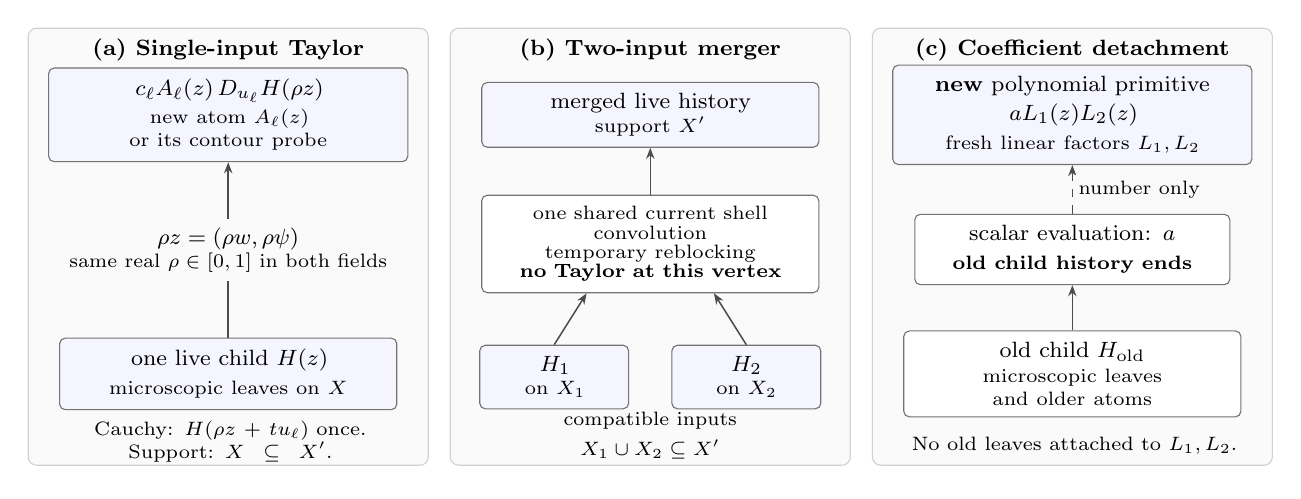
\begin{tikzpicture}[
  x=1cm,y=1cm,
  font=\footnotesize,
  history box/.style={draw=black!55,rounded corners=2pt,fill=white,
    align=center,inner sep=4pt},
  history live/.style={history box,fill=blue!4},
  history edge/.style={-{Stealth[length=4pt]},draw=black!70,line width=.55pt},
  history note/.style={align=center,font=\scriptsize},
  history title/.style={font=\footnotesize\bfseries,align=center}
]
  \foreach \x in {0,5.36,10.72}
    \draw[draw=black!18,fill=black!2,rounded corners=3pt]
      (\x,0) rectangle ++(5.08,5.55);

  \node[history title] at (2.54,5.27) {(a) Single-input Taylor};
  \node[history live,text width=4.28cm] (htout) at (2.54,4.45)
    {$c_\ell A_\ell(z)\,D_{u_\ell}H(\rho z)$\\[2pt]
     \scriptsize new atom $A_\ell(z)$\\[-1pt]
     \scriptsize or its contour probe};
  \node[history live,text width=4.00cm] (htin) at (2.54,1.16)
    {one live child $H(z)$\\[1pt]
     \scriptsize microscopic leaves on $X$};
  \draw[history edge] (htin.north) -- (htout.south)
    node[midway,fill=black!2,align=center,inner sep=3pt]
      {$\rho z=(\rho w,\rho\psi)$\\[-1pt]
       \scriptsize same real $\rho\in[0,1]$ in both fields};
  \node[history note,text width=4.70cm] at (2.54,.30)
    {Cauchy: $H(\rho z+t u_\ell)$ once.\\
     Support: $X\subseteq X'$.};

  \node[history title] at (7.90,5.27) {(b) Two-input merger};
  \node[history live,text width=4.00cm] (hmout) at (7.90,4.45)
    {merged live history\\[-1pt]
     \scriptsize support $X'$};
  \node[history box,text width=4.00cm,font=\scriptsize] (hm) at (7.90,2.81)
    {one shared current shell\\[-1pt]
     convolution\\[-1pt]
     temporary reblocking\\[-1pt]
     \bfseries no Taylor at this vertex};
  \node[history live,text width=1.61cm] (hminone) at (6.68,1.12)
    {$H_1$\\[-1pt]\scriptsize on $X_1$};
  \node[history live,text width=1.61cm] (hmintwo) at (9.12,1.12)
    {$H_2$\\[-1pt]\scriptsize on $X_2$};
  \draw[history edge] (hminone.north) -- ([xshift=-23pt]hm.south);
  \draw[history edge] (hmintwo.north) -- ([xshift=23pt]hm.south);
  \draw[history edge] (hm.north) -- (hmout.south);
  \node[history note] at (7.90,.57) {compatible inputs};
  \node[history note] at (7.90,.20) {$X_1\cup X_2\subseteq X'$};

  \node[history title] at (13.26,5.27) {(c) Coefficient detachment};
  \node[history live,text width=4.28cm] (hdnew) at (13.26,4.45)
    {\textbf{new} polynomial primitive\\[1pt]
     $aL_1(z)L_2(z)$\\[1pt]
     \scriptsize fresh linear factors $L_1,L_2$};
  \node[history box,text width=3.72cm] (hdeval) at (13.26,2.74)
    {scalar evaluation: $a$\\[1pt]
     \scriptsize\bfseries old child history ends};
  \node[history box,text width=4.00cm] (hdold) at (13.26,1.16)
    {old child $H_{\rm old}$\\[1pt]
     \scriptsize microscopic leaves\\[-1pt]
     \scriptsize and older atoms};
  \draw[history edge] (hdold.north) -- (hdeval.south);
  \draw[history edge,dashed] (hdeval.north) -- (hdnew.south)
    node[midway,right,fill=black!2,inner sep=2pt,font=\scriptsize]
      {number only};
  \node[history note,text width=4.70cm] at (13.26,.25)
    {No old leaves attached to $L_1,L_2$.};
\end{tikzpicture}
\caption{Selected history operations from
Definition~\ref{xyh:history-definition} and Lemma~\ref{xyh:history}.
These are separate schematic rules; panel~(a) shows one selected Taylor
direction factor. Solid arrows carry live field dependence up to its
termination; the dashed arrow carries only an evaluated number.
Live microscopic supports only enlarge or unite, Cauchy differentiation
uses one shifted child, and detachment ends the old microscopic and atom
ancestry before new polynomial factors are formed.}
\label{xyh:history-figure}
\end{figure}

\begin{lemma}[Supports, collars, and overlap]\label{xyh:history}
Each live Gaussian root of Definition~\ref{xyh:history-definition} has
the following uniform properties. They also apply when that root is
completed. No assertion combines atom boxes or source squares of distinct
completed roots in the same forest.
\begin{enumerate}[label=\textup{(\alph*)}]
\item A support carrying microscopic leaves or atoms of the live root never shrinks: it is
replaced only by coarse closure or a union. No selected microscopic
factor of the same type occurs twice in one live root.
\item All fields in the live root can be represented on one ambient
stack of shell coordinates. Individual atom representations require a
fixed collar, whose width in current block units is bounded independently
of depth and $L$.
\item Atom boxes have bounded overlap at each birth scale, uniformly in
$L$ and history depth. The same holds for the fine-scale probe boxes of
one step.
\item If a Taylor operation after the shell ending at $S$ changes the
attenuation on one group of live microscopic leaves, then groups having
different relative changes have zero cross entries in the restricted
white tail $E_{\ge S}$.
\end{enumerate}
All assertions apply to an early-stopped root, reflected grids, and
the auxiliary torus.
\end{lemma}
\begin{proof}
Initially each selected vertex factor appears once at its vertex, and each
selected edge factor of a specified type appears once and contains its two
endpoints. Convolution takes closures, a residual keeps
the full temporary support, and products take unions. The only shrinking
operation is coefficient detachment in Definition~\ref{xyh:history-definition}(iii),
where the old Gaussian root, including its atoms, has ended. A new
polynomial begins with its own support and atoms. Scalar decorations
introduce no field, and choosing a summand or one contour derivative does
not copy a microscopic factor. This proves (a) inductively within each
root. A tilt factor and an
$F_b$ factor may use the same physical edge; the no-repetition assertion
is separate for each type, as required below.

For (d), fix a Taylor change at scale $S$. Its child is a single input, so
all live leaves in that child receive the same relative factor. For any
other leaf with a different factor, follow the branches to their first
product ancestor. If that product is formed at this regrouping, they
were distinct temporary objects and their original supports have
distance greater than $r_0S$. If it occurs later, the two unshrunk
ancestors are distinct compatible fine components, or distinct temporary
objects at that later step. Their distance is therefore greater than
the corresponding fixed radius times a scale at least $S$. There is no
case of differently changed live branches inside the same temporary
Taylor input: that input was linear. By (a), later closure cannot have
hidden an earlier nearby leaf. Choose $r_0$ larger than the range constant
in Equation~\eqref{xyh:white-resolution}. Its white tail then has the
asserted zero cross blocks. Unchanged leaves count as a group with
relative multiplier one.

Here is the collar induction needed for (b). If a newly emitted atom uses
$c_0$ birth-block widths and all inherited dependence uses $c_*$ old-block
widths, the new dependence is contained in
$c_0+c_*/L+c_{\rm st}$ current-block widths, with a fixed stencil allowance
$c_{\rm st}$. Fix $c_*=2(c_0+c_{\rm st})+1$; the required induction
inequality then holds for every $L\ge2$. Let $c_{\rm ker}$ bound the
relevant kernel range in current block units. The small-closure conclusion
of Lemma~\ref{rg:geometry} makes a support relocation at most one current
block, so fix $c_{\rm move}=1$ for that conclusion. Choose the temporary radius
$r_0>2c_*+c_{\rm ker}+4$ and the compatibility radius
$R>r_0+2c_{\rm move}+4$, increasing them if necessary for earlier
kernel ranges. The small-support threshold in Lemma~\ref{rg:geometry}
uses these fixed radii, and $L$ is then taken large enough for its
small-closure conclusion. The resulting fine small-support diameter is
fixed before this last choice of $L$, so the Fourier cutoff uses a fixed
number of coarse blocks. These separations
are the locality hypotheses used in the factorization proof of
Proposition~\ref{rg:partition-map}, with the present block collars in
place of its smaller microscopic collar. Before
compatible inputs meet, all their already integrated shells then have
zero cross covariance, including their atom dependence. The current
shell at a multiple-input convolution is shared from the outset.
Before products of temporary objects, use their stronger temporary
separation. Gaussian characteristic functions factor when these cross
blocks vanish; Fourier uniqueness proves factorization for the finite
complex Gaussian measures of the strict regularization. The limiting
factorization follows after the endpoint bounds below. This proves the
common-stack induction. When a finite-grid good piece is copied from the
plane, only equality of the restricted covariances is needed; the chosen
square roots need not be identical.

For (c), a selected Taylor term emits only its fixed number of direction
atoms at the upper birth scale, and only a single-input temporary object
emits them. Distinct batches in one final history are separated at that
birth scale by the same first-product-ancestor argument. In particular
an upper block may contain $O(L^2)$ fine inputs, but its multiple-input
convolution emits no new Taylor atoms: the old atoms retain their old
birth scales. A tensor is a normalized vertex/orientation sum; a selected
summand contains only its two linear factors, not a pair at every vertex.
The same observation applies to a localized quadratic assignment.
Products of these primitives have fine compatibility or temporary
separation. At a fixed scale there are only finitely many such types.
If a coefficient calculation ends, its older atoms end with it and are
not stacked on its newly assigned polynomial. Repeated opaque occurrences
of that coefficient add no atoms to the new root; if expanded, each copy
is checked on its own completed stack. At the microscopic scale
the list of primitive types and polynomial degrees is fixed. This proves
the bounded overlap without an $L^2$ loss. Probes have the same ancestry
and a fixed number per node. Reflections, periodic distance, and the
terminal harmonic piece do not alter any of these support arguments.
\end{proof}

For one shell introduce coordinates $x=(x_T,x_L),y$ with inverse
covariance
\[
 \begin{pmatrix}\mu I&i d_cJ\\i d_cJ^t&sI\end{pmatrix},
 \qquad Jy=(0,y),
\]
and fields $w_r=B_rx_T+D_rx_L$, $\psi_r=\Gamma_r^{1/2}y$,
$p_r=D_ry$. Use the same letter $J$ for the orthogonal embedding on the
complete stack. Each microscopic leaf and each atom has attenuation
one at birth; passing a Taylor node multiplies its future coupling in
both fields by the same number in $[0,1]$. It may eventually terminate.
Thus these scale weights have uniformly bounded variation.

\begin{lemma}[Contraction of the attenuated stack]\label{xyh:contraction}
Fix one live Gaussian root. On its distinct microscopic tilt edges, let
$R_wx,R_py$ be the attenuated
edge and gradient totals. On the distinct $F_b$ edges let $R_Fx$ be its
edge total. Then
\begin{equation}\label{xyh:contracting-maps}
 \|R_w\|\le1,\qquad\|R_p\|\le1,\qquad
 \|R_F\|\le1,\qquad R_wJ=R_p.
\end{equation}
\end{lemma}
\begin{proof}
Restrict the white kernels to the distinct edges under consideration and
write $A_r$ for their diagonal attenuations. The row covariance is
$\sum_rA_rE_rA_r$. If the history stops early, add the missing positive
tail with the last attenuation. Remove changes in reverse chronological
order. After all later changes have been removed, a change at $S$ leaves
a tail $P Q E_{\ge S}Q P$, where $P$ records all earlier factors and
$Q$ the new relative factors. By Lemma~\ref{xyh:history}(d), the restricted
tail is block diagonal between groups on which $Q$ differs. On each
block $Q=qI$ with $0\le q\le1$, whence
$QE_{\ge S}Q\preceq E_{\ge S}$. Congruence by $P$ preserves this order,
even when $P$ varies within a block. Removing every change leaves
$\sum_rE_r=I$. This proves the $R_w$ and $R_F$ bounds. Replacing
$D_rD_r^*$ by $E_r$ proves the $R_p$ bound. Finally the same attenuation
in both fields gives $R_wJ=R_p$ row by row. Deterministic probe and twist
backgrounds do not change these linear maps.
\end{proof}

\subsection{Finite Gaussian completion and endpoint bounds}

\begin{lemma}[Mixed completion and its Cameron bound]\label{xyh:mixed}
Fix one live Gaussian root. After incorporating its microscopic quadratic
tilts, let $\Theta$ be their diagonal matrix of strengths in $[0,1]$.
The stacked inverse covariance has blocks
\begin{equation}\label{xyh:completed-precision}
 \begin{gathered}
 \begin{pmatrix}M&iH\\iH^t&S_0\end{pmatrix},\qquad\text{where}\\
 \begin{aligned}
 M&=\mu I-s_{11}R_w^t\Theta R_w,\\
 H&=d_cJ-s_{12}R_w^t\Theta R_p,\\
 S_0&=s(I-R_p^t\Theta R_p)\succeq0.
 \end{aligned}
 \end{gathered}
\end{equation}
Its Gaussian reweighting determinant has modulus at most $e^{CN_h}$.
Define
\begin{equation}\label{xyh:completion-matrices}
 D=(S_0+H^tM^{-1}H)^{-1},\quad C'=M^{-1}HD,
 \quad V=M^{-1}-C'D^{-1}(C')^t\succeq0.
\end{equation}
Then $M,D$ are uniformly close to the identity. A source $e^{i(Y,y)}$
contributes $e^{-(Y,DY)/2}$, and the remaining $x$ integral is a real
Gaussian with covariance $V$ evaluated at mean $C'Y$.
If $I=\Im Y$, the imaginary evaluation shift $iC'I$ may be replaced by
$iJI$ at cost at most $e^{C\|I\|^2}$, leaving the remaining real
Gaussian estimate unchanged.
\end{lemma}
\begin{proof}
Equation~\eqref{xyh:completed-precision} follows by substituting the
linear maps of Lemma~\ref{xyh:contraction} into the quadratic tilts.
Those contraction bounds imply $M=I+O(|s_\bullet|)$ and
$H=J+O(|s_\bullet|)$, while $0\preceq S_0\preceq sI$.
The Schur complement is therefore positive and close to $I$.
The perturbation of the untilted inverse covariance has rank at most a
fixed multiple of the number of tilt leaves. The untilted covariance has
bounded operator norm, including as $s\downarrow0$; its product with the
precision perturbation is small in operator norm. Thus the determinant
ratio is a product of at most $CN_h$ numbers of modulus in a fixed
neighborhood of one. This proves its bound independently of the number
of unused Gaussian coordinates.

For $S_0>0$, integration in $y$ or direct block inversion gives covariance
\[
 \begin{pmatrix}V&-iC'\\-i(C')^t&D\end{pmatrix}.
\]
Its characteristic function with a $y$ source proves the asserted mean
and exponential factor. Positivity of $V$ is the Schur-complement
identity
$V^{-1}=M+HS_0^{-1}H^t$; limits prove the positive semidefinite case.

Let $A=I-R_p^t\Theta R_p$, $\Delta=C'-J$. Using $R_wJ=R_p$ gives
\begin{align*}
 H^t\Delta
 &= (I-S_0D)-(d_cI-s_{12}R_p^t\Theta R_p)\\
 &= -A(sD+s_{12}I).
\end{align*}
For nonsingular $A$ and $s>0$ the Cameron square satisfies
\[
 \Delta^tV^{-1}\Delta
 =\Delta^tM\Delta+
 (sD+s_{12}I)^t A(sD+s_{12}I)/s\preceq CI,
\]
since $s_{12}^2/s\le d_*^{-1}$. The same inequality holds on the
supported space by approximation when $A$ is singular. At $s=0$ one has
$s_{12}=0$ and $H^t\Delta=0$, which is exactly the required range
condition for the possibly singular $V$.

Translate the real Gaussian variable by $i\Delta I$. Its density changes
by a phase of modulus one and the factor
$\exp(\|\Delta I\|_{V^{-1}}^2/2)\le e^{C\|I\|^2}$.
The remaining evaluation shift is $iJI$. The entire-function translation
is justified first with positive covariance and strict compensation by
Equation~\eqref{xyh:primitive-bound}, then by the same Gaussian majorant
on the supported limiting space. Linear $x$-source factors can be left
in the integrand during this translation; their extra deterministic
factor is bounded by Cauchy--Schwarz using their source norm. No
unrestricted imaginary Gaussian is substituted into $F_b$.
\end{proof}

We next specify the deterministic decorations retained inside a live-root
integral. A polynomial contour has fixed radius and its atom factor has
the form $e^{t[A(Z)+d_A]}$, where $Z$ is its attenuated variable field.
The deterministic value $d_A$ is part of this exponential. Likewise,
deterministic offsets remain in the arguments of $F_b$ and of the
microscopic quadratic tilts. These decorations are not structural
numerical coefficients, even after the contour variables have been fixed.
Only the following rules introduce them: the fixed Cauchy probes in a
selected Taylor calculation; the intrinsic microscopic offsets in
Equation~\eqref{xyh:offsets}; and one good-support transport defined
below. They cannot contain an arbitrary numerical multiplier.

Every retained event of a live root carries at most one physical source
decoration. Each root also has a tag state. The unmarked construction
omits the physical-source record, so its roots start untagged. A present
intrinsic physical-source record tags its root at birth even when all its
numerical offsets vanish. A good-support transport is defined only on an
untagged root and makes it tagged. The
empty root stays untagged. A representation is untagged when every
selected live root is untagged. A product root is tagged if any input root is
tagged, and Taylor operations never clear that state, even when a current
attenuation becomes zero. The transport leaves every opaque completed
coefficient occurrence untouched. Subsequent convolution and Taylor
operations carry existing physical decorations without applying that
transport again; new Taylor atoms are outside the differentiated child
and do not receive its same-step probe. Completion ends all the root's
decorations and its tag state. A new polynomial primitive with a completed
numerical coefficient starts with new atoms and its own untagged state.

For the early class there is a fixed constant $C_{\rm tag}$ such that the
total deterministic offset at each selected microscopic edge and $|d_A|$
at each atom are at most $C_{\rm tag}$. Physical scalar phase decorations
are real, so their exponentials have modulus one. The constant is uniform
for at most two signed sources, and for the early part of each fixed
separated source configuration specified below. This class also includes
the accumulated Cauchy probe decorations. Their uniform bound follows
directly from the birth normalization. If $A$ was born at $h$ and $u$ is
a later normalized probe at scale $m\ge h$, then
\[
 |A(u)|\le C h/m.
\]
For scalar atoms subtract the probe's anchor value and use constant
annihilation; for edge atoms use the extra factor $h$ in the test norm.
There are a fixed number of probes per passing scale, and
$\sum_{m\ge h,\ m/h\text{ a power of }L}h/m\le(1-L^{-1})^{-1}$.
At microscopic edges the corresponding sum is bounded by
$C\sum_{m\ge1}m^{-1}$ over the geometric scales. Thus these rules give
the asserted fixed bounds. The exception is a probe paired with an
original charge phase. At a Taylor node with current charge array $k$
this contributes at most
\begin{equation}\label{xyh:phase-probe-cost}
 \exp\{C h_m(k;X)\}.
\end{equation}
These factors are retained separately and paid in Lemma~\ref{xyh:budget}.

Here are the bounds for the physical decorations. On a good support write
$\Lambda=(\Lambda_w,\Lambda_\psi)$, where
$\Lambda_w=-i d_c\eta/\mu$ and the real local lift satisfies
$\partial\Lambda_\psi=\eta$ and agrees with $\vartheta$ modulo its period.
Let $A$ be an atom born at $h$, and let $\mathcal C_A$ be its fixed
expanded birth collar. Write $v^\flat$ for the physical representative of
$v$ under the prescribed wall reflections, with $v^\flat=v$ on the physical
grid. At every point $v\in\mathcal C_A$, the high-order source bound is
\[
 |\nabla^j\eta(v)|\le C e^{C_0(j+1)^2}b^{-1/2}
       \sum_i(1+\operatorname{dist}(v^\flat,x_i))^{-1-j}.
\]
This is a pointwise bound on the collar; it does not choose one source
as nearest throughout that collar. Put
$d_i(A)=\inf_{v\in\mathcal C_A}\operatorname{dist}(v^\flat,x_i)$.
When the collar has good clearance, the test normalization and the bound just displayed give
\[
 |A(\Lambda)|\le Cb^{-1/2}\sum_i\frac{h}{1+d_i(A)}.
\]
For a scalar atom, its zeroth order is a path of length $Ch$ times the
gradient bound; its order-$j$ contribution from source $i$ is bounded by
$C b^{-1/2}e^{-(K_0-C_0)j^2}(h/(1+d_i(A)))^j$. For an edge atom the same
calculation uses $h^{j+1}\nabla^j\eta$. The good clearance bounds
$h/(1+d_i(A))$ by a fixed constant, so the higher orders are absorbed
by the test weights. In particular, suppose the current support has
clearance $Hm$ and its inherited collars extend at most $c_{\rm col}m$
from its hull, with $H>c_{\rm col}$. Then
$d_i(A)\ge(H-c_{\rm col})m$. For one or two sources the bound for an old
atom of birth size $h\le m$ is therefore $Ch/m$.

For $k_{\rm src}$ sources at mutual distance at least
$\epsilon M_{\rm box}$, call an atom early when its own birth size obeys
\begin{equation}\label{xyh:early-source-scales}
 Lh\le c\epsilon M_{\rm box}/(1+k_{\rm src}).
\end{equation}
Choose $c$ so the birth collar has diameter less than
$\epsilon M_{\rm box}/4$. At each folded point of that collar at most one source
is within $\epsilon M_{\rm box}/3$; the identity of that source may vary
with the point. Good clearance bounds its contribution by $C$, and the
other sources contribute at most
$Ck_{\rm src}h/(\epsilon M_{\rm box})$. Taking the pointwise supremum
therefore gives
\[
 |A(\Lambda)|\le C\left(1+
       \frac{k_{\rm src}h}{\epsilon M_{\rm box}}\right)\le C
\]
for every early atom. This still applies if its first transport occurs
on a later good support, because it tests the lift on $\mathcal C_A$.
At a microscopic edge the same pointwise argument uses
$(1+\operatorname{dist}(v^\flat,x_i))^{-1}\le1$ for the possible near source.
It gives a uniform intrinsic offset for at most two sources at every
volume and for each fixed separated configuration in all sufficiently
large volumes. No local scalar lift is imposed in a defect core; its
intrinsic scalar phases remain real.

For clarity, transport acts on a selected untagged live root by substituting
$z+\Lambda$ for its current field argument, and acts as the identity on an
empty root. Call it an admissible early transport when every induced
offset satisfies the fixed early bounds above; in the separated-source
case this is invoked only when all its atom birth sizes are early.
Write an old atom's factor as
$e^{t[A(Z_<+\tau_A z)+d_A]}$, where $Z_<$ contains its earlier
shell fields and $\tau_A\in[0,1]$ is its current coupling. The factor becomes
\[
 e^{t[A(Z_<+\tau_A z)+d_A+\tau_A A(\Lambda)]}.
\]
The new bounded term stays in the decorated endpoint integrand. It is
not factored into the structural numerical coefficient. The analogous
rule adds the attenuated physical offsets at original microscopic leaves
and a real phase at original charges. A later defect Taylor substitution
$z\mapsto\rho z+t'u$ changes this atom factor to
$e^{t[A(Z_<+\tau_A\rho z)+d_A+\tau_A A(\Lambda)+\tau_A t'A(u)]}$.
The physical tag stays fixed,
the future coupling is multiplied by the real $\rho$, and the new probe
increment is covered by the summable $h/m$ bound above. This proves
closure of the early decoration class under subsequent local operations.

The remaining birth sizes satisfy
$h>c\epsilon M_{\rm box}/[L(1+k_{\rm src})]$. In a finite box, bounded
overlap gives at most $C(M_{\rm box}/h)^2$ atoms of each such size in one
live root, including the fixed reflection multiplicity. There are only
$O_{k_{\rm src},\epsilon}(1)$ such scales. Hence their total number is
at most $C_{k_{\rm src},\epsilon,L}$, independently of the earlier depth.
Good clearance still gives $|A(\Lambda)|\le Ck_{\rm src}$ for each such
event. For these late events only, factor the possibly large deterministic term
$e^{t\tau_A A(\Lambda)}$ into an explicitly recorded late numerical
factor. The variable source remains $tA(Z)$ with the original fixed
contour radius. The product of the late factors is bounded by a constant
depending on the fixed configuration per live root. It does not change
any earlier event weight. Opaque completed coefficients are not
transported, and no singular lift is imposed on a new defect-core tensor.

Finally a fixed-radius polynomial contour produces a bounded linear
Gaussian atom. Within one live root Lemma~\ref{xyh:history} supplies the
overlap hypothesis of Lemma~\ref{xyh:atoms}, so all their source squares
sum to at most $CN_h$. Completing a decorated microscopic tilt produces
sources $R_w^t\Theta a$ or $R_p^t\Theta a$ with bounded coefficients at
each selected edge. Lemma~\ref{xyh:contraction} gives the same square
bound, or these sources may be regarded as edge atoms born at size one.
The deterministic early atom decorations have modulus at most
$e^{C N_h}$ after all fixed-radius contours, while physical phase
decorations have modulus one. These are uniform endpoint bounds for the
specified decoration class, not changes of its structural coefficients.

\begin{lemma}[Estimate for an evaluated history]\label{xyh:endpoint-estimate}
Fix one live Gaussian root with an admissible early decoration record as
defined above. Let $n_F$ be its number of original $F_b$ leaves, and let
$Y_o$ be its real original charge source on its shell stack. Keep all
admissible early decorations inside the endpoint integral. Omit only its
structural numerical coefficient, its opaque completed coefficient
occurrences, its explicitly extracted late numerical factors, and the
phase-probe factors in Equation~\eqref{xyh:phase-probe-cost}. Then the
resulting fully evaluated integral $\mathcal I_h^{(0)}$ obeys
\begin{equation}\label{xyh:endpoint-bound}
 |\mathcal I_h^{(0)}|\le b^{-n_F}\exp\{CN_h-c\|Y_o\|^2\}.
\end{equation}
The same bound holds for normalized fixed-order directional derivatives,
with their bounded number of contour events included in $N_h$. Constants
are uniform over the admissible early decoration class, strict
regularizations, the permitted small parameters, depth, and domain.
The omitted late numerical factors have the separate fixed-configuration
bound proved after Equation~\eqref{xyh:early-source-scales}. Each other
completed root in the forest satisfies its own copy of this estimate.
\end{lemma}
\begin{proof}
The fixed-radius atom contours and the bound $|d_A|\le C_{\rm tag}$ give
$\prod_A|e^{t_A d_A}|\le e^{CN_h}$ within this endpoint integral.
Physical scalar phases have modulus one. The decorated microscopic edge
offsets are uniformly bounded. These facts use exactly the admissible
decoration rules and do not move any early factor into the structural
coefficient.

On a shell acting on current phase charges $k$, the original source is
$\Gamma_r^{1/2}k$ in the $y$ coordinates. It is real because all previous
charge attenuations were real. Write $Y=Y_o+Y_a$; the preceding source
estimates give $\|Y_a\|^2\le CN_h$, and every linear $x$ source has the
same bound. Lemma~\ref{xyh:mixed} reduces the imaginary evaluations at
$F_b$ leaves to the attenuated outputs of $JI$, $I=\Im Y_a$, together
with bounded deterministic offsets. By Lemma~\ref{xyh:moment-bound}, their
values $v_e$ obey
$\sum_e|v_e|^p\le N_h(Cp)^p$, $p\ge2$. Consequently
\begin{align}\label{xyh:imaginary-payment}
 \sum_e |v_e|^2 e^{|v_e|/\sqrt b}
 &\le N_h\sum_{k\ge0}
 \frac{C^{k+2}(k+2)^{k+2}}{k!\,b^{k/2}}
 \le CN_h
\end{align}
for all sufficiently large fixed $b$. The ratio
$(k+2)^{k+2}/k!$ is bounded by an exponential in $k$ times a fixed
polynomial, so the displayed series converges. Bounded offsets add at
most $C$ per leaf. Thus the imaginary growth term in
Equation~\eqref{xyh:primitive-bound} costs $e^{CN_h}$.

Choose $\kappa_1$ strictly between $\kappa_0$ and $1/2$. Small parameter
size and Lemma~\ref{xyh:contraction} give a fixed $\nu>0$ such that
\begin{equation}\label{xyh:gaussian-slack}
 2\kappa_1R_F\{V+C'D^{-1}(C')^t\}R_F^t
   =2\kappa_1R_FM^{-1}R_F^t\preceq(1-\nu)I.
\end{equation}
For a real Gaussian $\xi$ of covariance $\Sigma=R_FVR_F^t$, completing
the square in
$\E e^{\kappa_1\|\xi+R_FC'Y_o\|^2}$ gives determinant
$\det(I-2\kappa_1\Sigma)^{-1/2}$, at most $e^{Cn_F}$.
Its shifted-mean exponent is
$\kappa_1\langle R_FC'Y_o,(I-2\kappa_1\Sigma)^{-1}R_FC'Y_o\rangle$.
Equation~\eqref{xyh:gaussian-slack}, or its Schur complement, bounds this
by $(1-\nu)(Y_o,DY_o)/2$ after decreasing $\nu$ if necessary.
It therefore leaves a fixed part of the charge exponential
$e^{-(Y_o,DY_o)/2}$ unspent.

Means from $Y_a$ and deterministic offsets have square $O(N_h)$ on the
evaluation edges. The difference $\kappa_1-\kappa_0$ absorbs them with
$e^{CN_h}$, using $2|uv|\le\delta u^2+\delta^{-1}v^2$. The same
inequality absorbs cross terms in $-\Re(Y,DY)/2$, and linear real
Gaussian sources, with an arbitrarily small additional fraction of the
retained charge square. Their source squares are $O(N_h)$; Gaussian
integration or a small H\"older enlargement gives $e^{CN_h}$. Since
$D$ is uniformly positive, the remaining suppression is
$e^{-c\|Y_o\|^2}$. Each branch factor contributes the separate
$b^{-1}$ in Equation~\eqref{xyh:primitive-bound}. Polynomial derivatives
use their fixed circles and add only a bounded number of source atoms.
This proves Equation~\eqref{xyh:endpoint-bound} in strict regularization,
with all constants independent of that regularization.
\end{proof}

\subsection{Charge budgets and a composable positive size}

\begin{lemma}[Simultaneous charge payment]\label{xyh:budget}
There are fixed choices of sufficiently large $L,b_0$ and a constant
$c'>0$ such that all phase-probe costs in one generated live root, a specified
bounded final smooth-test cost, and a factor $L^{-4}$ at every small
charged linear step can be included simultaneously in
Equation~\eqref{xyh:endpoint-bound}. Writing $\mathcal I_h$ for the
integral with those phase-probe factors restored, this leaves
\begin{equation}\label{xyh:paid-bound}
 |\mathcal I_h|\le
 C^{N_h}b^{-n_F}L^{-4n_{\rm ch}}
       \exp\{-c'b\textstyle\sum_vq_v^2\}
\end{equation}
apart from its structural numerical coefficient, opaque completed
coefficient occurrences, and explicitly extracted late factors. Here
$q_v$ are the original nonzero integral charge leaves of this root and
$n_{\rm ch}$ counts only its indicated single-input charged steps. The
admissible early decorations remain inside the evaluated integral.
\end{lemma}
\begin{proof}
Fix one selected live root, rather than the sum of its alternatives or
the forest of its separately completed coefficient dependencies.
At a charge-carrying node let $H=h_m(k;X)$ be the incoming test budget.
At a merger budgets add subadditively by test restriction and the
triangle inequality. Reblocking without localization is nonincreasing
by Equation~\eqref{xyh:test-coarsening}. At a neutral Taylor node its
real attenuation $\rho\in[0,1]$ gives
\[
 H_{\rm out}\le\rho(C/L)H,\qquad
 H-H_{\rm out}\ge(1-C/L)H.
\]
Thus a fixed multiple of this decrease pays
Equation~\eqref{xyh:phase-probe-cost}. At termination the remaining budget
is consumed, which also permits bounded final test directions.

For a charged small linear node put $Q=\sum k\ne0$, $q=|Q|$,
$\ell=\log L$, and let $\Gamma$ be its shell. Choose an anchor $v$ in
its support. Lemma~\ref{xyh:kernels}, summing its positive-order binary
bounds, shows that $\Gamma(\cdot,v)-\Gamma(v,v)$ on the local support
and collar is a fixed multiple of a fine test. Consequently
\[
 d:=\Gamma(v,v)\ge c_0\ell,\qquad
 |(k,\Gamma e_v)-Qd|\le C_1H.
\]
Fix $\epsilon=c_0/(2C_1)$ when $C_1>0$. If $H\le\epsilon q\ell$,
positive-semidefinite Cauchy--Schwarz gives
\begin{equation}\label{xyh:energy-alternative}
 (k,\Gamma k)\ge\frac{|(k,\Gamma e_v)|^2}{d}
       \ge\frac{q^2d}{4}\ge c q^2\ell.
\end{equation}
If $C_1=0$ this conclusion holds without a case split. Otherwise, for
$H>\epsilon q\ell$, Equation~\eqref{xyh:test-coarsening} and choices
$C/L\le1/2$, $\ell\ge4/\epsilon$ give
\begin{equation}\label{xyh:potential-alternative}
 H-H_{\rm out}\ge(1-C/L)H-q\ge H/4
                         \ge(\epsilon/4)q\ell.
\end{equation}
At all other nodes the first inequality in
Equation~\eqref{xyh:test-coarsening} is retained; thus no negative
budget decrease is hidden in this dichotomy.

The sum of child budgets minus the parent budget is a nonnegative
potential loss at every node. Summing these losses over this live root,
including the final retained budget, gives at most its original leaf
budget
\begin{equation}\label{xyh:initial-budget}
 H_{\rm leaf}\le C\mathfrak p\sum_v|q_v|.
\end{equation}
Only neutral total charges are multiplied by a Taylor attenuation.
Mergers add totals, so every nonzero sector total remains in
$\mathfrak p\Z$, even though individual entries inside a neutral branch
may cease to be integral multiples. Hence $q\ge\mathfrak p$ at every
recorded charged node. A fixed potential multiplier pays both neutral
probes and $4\ell$ at each node of
Equation~\eqref{xyh:potential-alternative}, once $b$ is large.

The alternative using shell energy requires a separate account. At the
shell of a recorded charged step, its temporary branch was a single
input. Every other live charge group in the eventual combined live root
is either another temporarily separated object at this step or first
joins at a later product ancestor. Lemma~\ref{xyh:history}(a),(d), with
the scalar shell range included in the radius choice, gives zero
cross-covariance between that charged branch and every other such group
on this shell. Thus its scalar energy splits off exactly, with a
nonnegative remaining square. Two selected branches at that shell are
mutually separated as well. Different recursion levels use disjoint
shell coordinates. A later Taylor attenuation changes future fields
only, so it does not alter a payment on an already integrated shell.
Writing $\mathcal E$ for the sum of the selected energies and $E_0$ for
the first-piece square, we have
\begin{equation}\label{xyh:disjoint-reserves}
 E_0=\gamma\mathfrak p^2\sum_vq_v^2,
 \qquad E_0+\mathcal E\le\|Y_o\|^2.
\end{equation}
This is a separation statement about generated single-input histories;
positivity alone would not allow one to split arbitrary charge squares.

Let $c$ be the constant in Equation~\eqref{xyh:endpoint-bound}. Choose a
fixed multiplier $D_0'$ large enough for all potential payments and the
specified final normalized tests. Since $|q_v|\le q_v^2$ for nonzero
integers, increasing $b$ yields
\[
 D_0'H_{\rm leaf}\le(c/4)E_0.
\]
Equations~\eqref{xyh:energy-alternative} and $q\ge\mathfrak p$ similarly
give $4\ell N_E\le(c/4)\mathcal E$, where $N_E$ counts the energy-paid
steps. These fixed allocations use disjoint portions of
Equation~\eqref{xyh:disjoint-reserves}; a fixed positive fraction of
$E_0$ and of the full source square remains. It supplies the microscopic
Gaussian in Equation~\eqref{xyh:paid-bound}. Detached scalar calculations
have their own completed integrals and are absent from this live source
square. Reusing an evaluated scalar multiplies its established bound once
per opaque occurrence; it does not reinsert any charge leaf or shell
reserve. If the occurrences are expanded, apply this proof separately to
each completed root and multiply the resulting bounds. No joint overlap
or charge-square assertion across those roots is used.
\end{proof}

\begin{proposition}[The exact XY activity calculus]\label{xyh:calculus}
Fix the covariance construction and the local partition map above.
Choose the fixed support and collar clearances, small-support threshold,
and $K_0$ first; then choose sufficiently large dyadic $L$, the polymer
weight as in Proposition~\ref{rg:partition-map}, a sufficiently small
parameter neighborhood, and finally sufficiently large $b$. Within
Equation~\eqref{xyh:permitted-parameters} the original XY integrals admit
positive representation sizes with all the following properties. Write
$\mathsf s_X(\mathcal R)$ for the size of a specified representation on
$X$, and $\|\mathcal R\|_A=\sup_X A^{|X|}\mathsf s_X(\mathcal R)$.
\begin{enumerate}[label=\textup{(\roman*)}]
\item An $F_b$ leaf costs $C/b$; a nonzero charge $q$ costs
$C e^{-cbq^2}$, summable over $q\ne0$; the linear microscopic
compensation costs $C|s_\bullet|$, and its nonlinear remainder costs
$C|s_\bullet|^2$. A full-block tensor costs $C|t|$, and a localized
polynomial costs a constant times its coefficient on normalized
$m$-scale directions.
\item Convolving a compatible product multiplies its input sizes, up to
a fixed factor per input. Temporary exclusions, relocation, scalar
normalizer decorations, and separation into a singleton tensor and
remainder are exact. The animal and placement sums obey
Proposition~\ref{rg:partition-map}; hence all multiple-input and
normalizer corrections are quadratic in the input sizes.
\item For a small single neutral linear input of size $u$, localization
has normalized coefficients at most $Cu$ and remainder size
$CL^{-3}u$ in the even bulk after constant and quadratic subtraction,
$CL^{-2}u$ at an even wall after constant subtraction, and $CL^{-1}u$
at a defect after constant subtraction. Each small charged single-input
step has size at most $CL^{-4}u$. Constants in these local gains do not
grow with sufficiently large $L$.
\item Sizes bound terminated evaluations and fixed-order Cauchy
derivatives with bounded smooth normalized backgrounds. In finitely many
normalized source directions the evaluated expressions are jointly
holomorphic on fixed bounded polydiscs, with the corresponding Cauchy
bounds after adding their finitely many probe events. They apply to
copied good pieces, their one-time translations to defects, and the
intrinsic offsets of Equation~\eqref{xyh:offsets}. For fixed separated
sources, the lower bound on $b$ is independent of their number; only the
boundedly many late numerical event costs may depend on the fixed source
configuration. If $T_\Lambda$ is an admissible early transport of an
untagged representation, then for any $A_U\ge A_D>0$, before support relocation
\[
 \mathsf s_X(T_\Lambda\mathcal R)=\mathsf s_X(\mathcal R),\qquad
 A_D^{|X|}\mathsf s_X(T_\Lambda\mathcal R)
 \le (A_D/A_U)^{|X|}\|\mathcal R\|_{A_U}.
\]
The transport leaves every opaque completed coefficient occurrence
unchanged and is not defined on an already tagged live root.
\item Every finite-depth activity, assigned coefficient, and normalized
partition identity is continuous in the permitted parameters, including
at $s=d_*s_{12}^2$ and at $s=0$, as long as its scalar normalizers are
nonzero. The statement holds on the plane at finite support, on finite
reflected grids, and on auxiliary tori with terminal transverse harmonic
directions. The bulk tensor and its local recursion are the same in all
these settings wherever the calculation has the required clearance.
\end{enumerate}
\end{proposition}
\begin{proof}
For a specified representation write each selected term in the form
\[
 c_h(\alpha)\,\ell_h(\alpha)
       \left(\prod_{\nu=1}^{m_h}a_{h,\nu}\right)
       \mathcal I_h(z;\mathbf d_h,\alpha).
\]
Here $h$ is its unique live root, or the empty root with integral one.
The variables $\alpha$ range over the compact Taylor and contour
parameter spaces with their positive product measure. The structural
coefficient $c_h$ contains the displayed parameter powers, finite
averaging coefficients, Fourier/Taylor direction weights, and contour
kernel factors. The factor $\ell_h$ is only the explicitly extracted
late numerical product defined above, and equals one when there are no
such events. The $a_{h,\nu}$ are opaque occurrences of previously
completed coefficients. The admissible early record $\mathbf d_h$ and
the generated phase-probe factors paid by Lemma~\ref{xyh:budget} stay
inside $\mathcal I_h$ and are not part of $c_h$ or $\ell_h$.

Give the live root the weight
\begin{equation}\label{xyh:representation-weight}
 W(h)=C_*^{N_h}\,b^{-n_F}
 \exp\{-c_*b\textstyle\sum_vq_v^2\}\,L^{-4n_{\rm ch}},
\end{equation}
with $W=1$ for the empty root. All counts and charges in this display
belong only to $h$. If $a$ has a chosen completed representation, let
$\mathsf m(a)$ be the bound supplied by this same rule at its earlier
evaluation, on the source domain where the size will be used. A size at
one fixed source point may instead use the exact modulus $|a|$ there.
For a uniform estimate or a later Cauchy formula on a source polydisc,
$\mathsf m(a)$ must be a completed size uniform on that polydisc, or
another proved bound for the supremum of $|a|$ there; a modulus at one
point does not suffice. Equivalently one may differentiate $a$ in its
separately completed root and use that derivative's completed size.
These choices also apply when completed numbers are combined before
forming a new primitive. In particular each source-independent component
of the full unmarked tensor may use
$\mathsf m(t_{ab,j})=|t_{ab,j}|\le |t_j|_\infty$ after its evaluated
increments have been summed, preserving their cancellation. This choice
asserts no derivative bound in the real reference parameters; only their
continuity is used in (v). The acyclic coefficient dependence makes this
a finite-depth recursive definition. Set
\[
 \mathsf s_X(\mathcal R)=\sum_h\int
     |c_h(\alpha)|\,|\ell_h(\alpha)|
     \left(\prod_{\nu=1}^{m_h}\mathsf m(a_{h,\nu})\right)
     W(h)\,d\alpha.
\]
Choose $C_*$ sufficiently large and $c_*>0$ sufficiently small from the
bounds in Lemmas~\ref{xyh:endpoint-estimate} and~\ref{xyh:budget}, which
are uniform over the admissible early records and sufficiently large
$L$. Induction over coefficient evaluations then gives
$|a|\le\mathsf m(a)$ and makes this size a positive majorant of every
endpoint forest. No arbitrary numerical factor can be hidden in the
endpoint integral because its admissible records have the specified
generation rules and bounds.

The primitive bounds in (i) follow directly: polynomial
contours contribute a fixed number of atoms, and
Equation~\eqref{xyh:quadratic-remainder} has two explicit powers of
$s_\bullet$ and only a bounded tilt strength in its exponential.
A full tensor has normalized vertex averages: each selected summand
has two normalized atoms and coefficient $O(|t|)$.

When compatible live roots are concatenated, their live leaf lists and
actual event lists are disjoint. The common-stack construction joins them
into one live root, while their structural and late numerical factors
multiply and their lists of opaque coefficient occurrences concatenate.
At the final endpoint apply Equation~\eqref{xyh:paid-bound} once to the
concatenated live root, whose geometric properties were proved in
Lemma~\ref{xyh:history}. Thus no fresh $C^{N_h}$ is charged each time an
old root is convolved. Each opaque numerical coefficient is already
bounded at its own endpoint. In particular an inverse-normalizer term
$a_B^m$ has size $\mathsf m(a_B)^m$, and its absolute series is at most
$\mathsf m(a_B)/(1-\mathsf m(a_B))$ when $\mathsf m(a_B)<1$. If these
occurrences are expanded, they are $m$ separately completed roots and
their endpoint weights multiply; no common atom-overlap estimate is
applied to them.
This proves the product rule. The purely spatial enumeration in
Proposition~\ref{rg:partition-map} uses precisely these multiplicative
sizes: nonlinear inputs carry at least two factors, large supports use
the polymer weight gain, and the inverse scalar decorations use their
absolutely convergent small scalar series. It does not require a
pointwise norm at arbitrary remaining fields. This proves (ii).

For (iii) Taylor's integral formula of order $a$ contributes $a$ direction
arguments and a fixed number of contour events. Apply the exact
$CL^{-1}$ directional decomposition of Lemma~\ref{xyh:fourier} to each
argument before using Cauchy's formula. This gives $CL^{-a}$ in the
positive coefficient sum. The evenness assumption makes the linear
term vanish when $a=2$ or $3$. In the bulk, the quadratic Taylor term
has two arguments; replacing one by its affine approximation costs
$CL^{-2}$ and the other $CL^{-1}$, so the two-factor difference has
$CL^{-3}$. The affine polynomial itself is the assigned tensor
prescription of Equation~\eqref{xyh:tensor}. Its normalized coefficient
is a terminated history with bounded probes, hence costs $Cu$ by
Lemma~\ref{xyh:budget}. Scalar extraction is the same statement with
zero Taylor arguments. The charged gain is exactly the recorded factor
in Equation~\eqref{xyh:representation-weight}. Multi-input terms receive
no such Taylor or charged gain, consistently with both the grammar and
the quadratic counting rule.

For (iv), apply $T_\Lambda$ only to an untagged live root in the displayed
representation, and as the identity to an empty root, using the same
source domain and completed coefficient bounds. The transport rule changes
$\mathbf d_h$ inside $\mathcal I_h$ and leaves $c_h,\ell_h$, every $\mathsf m(a_{h,\nu})$,
and the event list defining $W(h)$ unchanged. Its own-birth bound proves
that the new record is admissible. The equality of representation sizes
in (iv) is therefore termwise in their defining nonnegative sums, before
any support relocation; multiplying by $A_D^{|X|}$ gives the displayed
comparison with the $A_U$ norm. In particular no factor per old event is
charged to a support weight. The endpoint bound for the transported
integrand is available because Lemma~\ref{xyh:endpoint-estimate} was
proved uniformly over these records. This is a comparison of the same
chosen representations, not merely a comparison of their endpoint values.
At finite strict regularization the factor-by-factor substitution is an
exact representation of the translated activity. The uniform majorants
used below pass this identity to the limiting evaluated expressions on
the bounded background domains used here.

The derivative claims in (iv) follow from the derivative version of
Lemma~\ref{xyh:endpoint-estimate} and the final-test allowance in
Lemma~\ref{xyh:budget}. A Cauchy derivative in a remaining field
direction acts on $\mathcal I_h$ with every opaque scalar occurrence
fixed. A derivative in a source parameter on which an opaque scalar
depends instead uses its uniform polydisc bound in the preceding
definition, or differentiates that scalar within its separately completed
root. Thus cutting a root never discards a source-parameter derivative.
The summable later-probe calculation proves that
a tagged root stays in the admissible class under further defect
operations. At late birth sizes only the separate factor $\ell_h$ changes;
its bounded number of events gives a fixed-configuration factor per live
root. It does not change an earlier event weight or an opaque completed
coefficient size. Thus the inverse-temperature threshold remains
independent of the fixed correlation order.

Finally fix a finite calculation depth and a finite geometry. All its
support choices and discrete Fourier direction decompositions are
finite; compact Taylor and contour parameters can be fixed independently
of a small parameter variation. Only the microscopic integral charge
indices remain unbounded. Before removing regularizations, all
identities are ordinary integrated identities of entire functions with
strict real-density integrability: the $x$ growth is below its Gaussian
threshold by Equation~\eqref{xyh:primitive-bound}, the real $y$ precision
is positive with strict compensation, and the mixed terms are imaginary
on real coordinates except for controlled lower-degree sources.
Lemma~\ref{xyh:mixed} proves the integrated formulas and
Lemmas~\ref{xyh:endpoint-estimate}--\ref{xyh:budget} give bounds uniform
as compensation becomes full. At fixed geometry the completion before
the Cameron estimate is also continuous: its real covariance $V$ may
become singular, but positive Gaussian measures converge to the measure
on its supported space, and its complex shifts are bounded for fixed
contour choices. The retained real-charge Gaussian square dominates the
remaining fixed-background costs, which grow only exponentially linearly
in the charge magnitudes. Thus dominated convergence removes charge
truncation and strict compensation at this fixed depth. The same
majorants hold uniformly on each smaller source polydisc, so integrating
Cauchy formulas proves holomorphy and convergence of source derivatives.
It also passes real parameter continuity to the limit. Scalar division is
continuous whenever its normalizer stays away from zero, as ensured in
the small-activity map. Plane calculations at finite depth use an
auxiliary large torus whose preterminal covariance entries agree on
all required supports, so the same reasoning applies there. This proves
(v) and completes the limiting justification promised in
Proposition~\ref{xyh:compensation}.
\end{proof}

\section{The XY flow, admissible tuning, and spin-field limit}
\label{xyf:section}

We apply the representation calculus of Proposition~\ref{xyh:calculus}
to the ordinary nearest-neighbor XY model.  Throughout this section,
\(b\) denotes spin inverse temperature,
\[
 \mu=1+s_{11},\qquad d_c=1+s_{12},\qquad s=s_{22},
 \qquad s\ge d_*s_{12}^2.
\]
The constant \(d_*>0\) will be chosen below.  The interaction includes
the compensating factor \(e^{+U(w,p)}\), with
\[
 U(w,p)=\frac12\sum_e
  \bigl(s_{11}w_e^2+2i s_{12}w_ep_e+s_{22}p_e^2\bigr),
 \qquad p=\partial\psi.
\]
The covariance prescription and the regularized interpretation at
\(s=s_{12}=0\) are those of Proposition~\ref{xyh:compensation}.
In particular, the prescription is not integration against a positive
joint law of \((w,\psi)\).  Positivity will be used only for the completely
restored vortex/transverse ensemble of Proposition~\ref{xyh:branch}.

\subsection{The exact recurrence}

For a full block \(B\), write
\begin{equation}
 \mathcal E_B(t)=\frac12\sum_e\mathrm{wt}_B(e)
 \bigl(t_{11}w_e^2+2i t_{12}w_e(\partial\psi)_e
                  +t_{22}(\partial\psi)_e^2\bigr).
 \label{xyf:tensor}
\end{equation}
Here \(\mathrm{wt}_B\) assigns half of an edge to each endpoint in \(B\).
Thus the weights sum to one when the blocks partition the whole grid.
The tensor norm is the maximum of the three coefficient absolute values.
The size of a remainder is the supremum over its supports of
\(A^{|X|}\) times its positive representation size.  Representation size
means the recursive sum in Proposition~\ref{xyh:calculus}, with each term
weighted by its live-root weight and the product of its opaque completed
coefficient sizes;
it is not a pointwise supremum over future complex Gaussian fields.

We record precisely which parts of that proposition enter the flow.
They hold uniformly in the number of integrated scales and in the
finite-grid size.  A microscopic \(F_b\) factor has size \(C/b\), a
nonzero charge has a summable bound \(e^{-cbq^2}\), and the nonlinear
part of a microscopic compensation factor has size \(C|s_\bullet|^2\).
A tensor singleton has size \(C|t|\).  Concatenating compatible histories
multiplies their sizes, up to a fixed constant per input.  On a small
\emph{linear} input, neutral localization gives the following gains:
\[
 \begin{array}{c|c|c}
 \text{class}&\text{subtracted polynomial}&\text{remainder gain}\\ \hline
 \text{bulk, even}&\text{constant and quadratic}&CL^{-3}\\
 \text{wall, even}&\text{constant}&CL^{-2}\\
 \text{defect}&\text{neutral constant}&CL^{-1}.
 \end{array}
\]
Every small charged linear input instead has gain \(CL^{-4}\).
The extracted coefficients, in normalized fine-scale directions, are
bounded by \(C\) times the input size.  The same history estimates bound
terminal evaluations and fixed smooth-source derivatives.  Finally,
local identities are exact, their finite-depth values are continuous in
the admissible parameters including the degenerate boundary, and their
field arguments are analytic in the source neighborhoods used below.

\begin{proposition}[Bulk recurrence]\label{xyf:recurrence}
For every sufficiently small fixed \(\theta>0\), the geometric
parameters, then \(L\), and then \(A\) can be chosen so that the exact
bulk activities have the decomposition
\[
 K_j(X)=\ind_{X=\{B\}}\mathcal E_B(t_j)+\mathcal P_j(X),
 \qquad t_0=(s_{11},s_{12},s_{22}).
\]
If \(r_j\) is their remainder size, then, while the quantities on the
right are small,
\begin{align}
 |t_{j+1}-t_j|_\infty&\le C r_j,\label{xyf:increment}\\
 r_{j+1}&\le\theta r_j+C_{L,A}(|t_j|_\infty+r_j)^2,
       \label{xyf:remainder}\\
 r_0&\le C_{L,A}\bigl(b^{-1}+|t_0|_\infty^2\bigr).
       \label{xyf:initial}
\end{align}
At every fixed depth these coefficients and the needed fixed field
derivatives are continuous on the set where the preceding bounds are
retained.  The recurrence also holds, with the same bulk tensors,
on an auxiliary torus of side \(F L^j\), through scale \(L^j\), if
the fixed integer \(F\) is sufficiently large.
\end{proposition}

\begin{proof}
Use the temporary-component, relocation, and constant-decoration
identities of Proposition~\ref{rg:partition-map}.  They are algebraic
identities for local activities, used with the enlarged fixed separation
radii proved in Lemma~\ref{xyh:history}. Their hypotheses here are finite
shell range, the retained temporary exclusions, one-step locality of
assigned pieces, and multiplicative bounds for compatible inputs.
Finite range follows from Lemma~\ref{xyh:kernels}; the history
construction supplies the other hypotheses, including the fact that
evaluated coefficients are scalar factors and do not retain their
extinct microscopic leaves.

For completeness, the relevant counts are as follows.  The maximum
fine-block count \(n_0\) of a small component and the connectivity radius
are fixed before \(L\).  The number of small animals containing a
specified fine block is therefore a constant.  A coarse block has
\(O(L^2)\) fine blocks, giving at most \(CL^2\) small linear inputs per
coarse output.  Their neutral and charged contributions have total
operator bound
\begin{equation}
 C L^2(L^{-3}+L^{-4})\le C/L.
 \label{xyf:bulkcount}
\end{equation}
In the neutral bulk quadratic remainder, replace each argument by its
affine approximation.  The two-factor difference is the sum of one
term with the first argument replaced and one with the second replaced.
The error direction has size \(C/L^2\) and the other direction size
\(C/L\), so each term has size \(C/L^3\).  The first-order term
vanishes because the full neutral projection is even under
\((w,\psi)\mapsto(-w,-\psi)\).  This explains the gain used in
\eqref{xyf:bulkcount} without assigning a Taylor gain to a nonlinear
convolution.

For a large input, the closure estimate leaves an exponential weight
gain at least \(A^{-|X|/2}\), after the fixed per-input history cost.
Taking \(A\) large after \(L\) makes the sum of its linear contributions
as small as prescribed.  To check nonlinear terms, root a compatible
family at a specified output block.  If it has \(q\) fine components
and a total of \(v\) fine blocks, a depth-first traversal of the fine
animals and a tree connecting their closures gives at most
\[
 C^v(CL^2)^{2q}
\]
choices.  The long jumps of that tree have range \(CL\) in fine-block
units.  For large components the weight gain sums these choices; the
total size of the small components is at most \(qn_0\).  Thus all
terms with \(q\ge2\) sum to
\(C_{L,A}(|t_j|+r_j)^2\).  Use a temporary output weight \(4A\) before
the constant-decoration step.  If \(a_B\) is the assigned constant,
then \(|a_B|\le C_{L,A}(|t_j|+r_j)\) and
\[
 d_B=(1+a_B)^{-1}-1=-a_B+O(a_B^2).
\]
Overlapping a decoration with an old occupied site costs at most two
choices, paid by the extra weight.  A decoration at a hole supplies a
factor \(|d_B|\).  The subset sum converges when
\(A\sup_B|d_B|<1/8\).  Every term containing an old component and a
decoration is quadratic; pure decorations are quadratic apart from
the displayed cancelling linear singleton.  Relocated multiple-object
terms are also quadratic, because their original temporary exclusions
are retained.  These counts prove the stated nonlinear bound.

The entire expectation of a tensor singleton is assigned to the coarse
singleton.  Its nonconstant part is exactly the same quadratic form;
its covariance contraction is a bounded constant.  At any specified
\emph{fine} block only a bounded number of small supports contribute
quadratic coefficients, each bounded by \(Cr_j\).  Averaging over
orientation signs and anchors and summing all fine blocks in a full
coarse block preserves translation and square symmetries.  Hence the
sum is precisely \(\mathcal E_B(t_{j+1}-t_j)\), with coefficient
bound \(Cr_j\).  There is no factor \(L^2\) in this coefficient:
the sum over fine sites is the edge sum already present in
\eqref{xyf:tensor}.  Complex conjugation combined with
\(\psi\mapsto-\psi\) makes the three extracted parameters real.
This proves \eqref{xyf:increment} and \eqref{xyf:remainder}.

At the first independent piece, the linear compensation factors give
the stated tensor and their designated covariance constants.
The remaining single primitives cost \(C/b\),
\(\sum_{q\ne0}e^{-cbq^2}\), or \(C|t_0|^2\).  Each edge has two
endpoints and only finitely many choices of primitive type.  The same
animal and decoration counts therefore give \eqref{xyf:initial}.

All these identities may first be performed with a finite Fourier
cutoff and strict covariance regularization.  At a fixed depth there
are finitely many geometric choices for each coefficient.  The charge
sums retain Gaussian domination; the contour and Taylor parameters
range over compact sets.  The completed finite-dimensional integrals
are continuous, including singular real Gaussian covariances, and
the scalar denominators stay away from zero.  The domination in
Proposition~\ref{xyh:calculus} consequently permits removing the
regularizations and taking parameter limits in each of these exact
identities.  It also permits fixed smooth-source Cauchy derivatives.
This proves the asserted continuity without a positivity assumption on
the mixed Gaussian pair.

For the torus take \(F\) larger than the fixed support, kernel, and
assignment clearances.  Every small input through the indicated scale
has an unambiguous lift to the plane, with its required neighborhood;
a winding input is large.  The local tensor assignments are therefore
identical to the plane assignments.  Large winding inputs obey the
large-support weight estimate.  The transverse harmonic directions
are added at the terminal integration, as prescribed in
Lemma~\ref{xyh:kernels}, and do not change any earlier local map.
\end{proof}

\subsection{The lower-face diagnostic}

The restriction \(s\ge d_*s_{12}^2\) is essential to the history bounds,
so a three-dimensional shooting argument must respect it.  We derive
the required boundary information from a positive finite ensemble.
On the auxiliary torus let
\[
 \mathrm d\nu(q,X)=Z^{-1}e^{-\|V_q\|^2/2}
     \prod_e f_b((X+V_q)_e)\,\mathrm d\gamma_{P_T}(X),
 \quad V_q=2\pi\sqrt b\,\partial Gq,
 \quad \sum_vq_v=0.
\]
Here \(P_T\) includes the harmonic transverse directions.  This is
a positive probability measure.  It is used only as the diagnostic
ensemble; no identification with a periodic XY spin law is required.

Choose a real torus function \(\varphi\) for which
\(g=\partial\varphi\) has norm one and is a lowest nonconstant
frequency mode.  For side \(M\), one may normalize a sine wave:
\(\|\varphi\|_\infty\le C\) and
\(\|\nabla^r\varphi\|_\infty\le C_rM^{-r}\).
Put
\[
 a=s/d_c,\qquad B_c=d_c+\mu a,
 \qquad w_{\rm ext}=(\lambda+i a\tau)g,
 \qquad \psi_{\rm ext}=\tau\varphi.
\]
Let \(Z(\lambda,\tau)\) be the fully integrated compensated partition
function evaluated at these external fields, with the same scalar
normalization as \(Z(0,0)\).  Denote the Hessian at zero of
\(\log[Z(\lambda,\tau)/Z(0,0)]\) by \(H\).

\begin{lemma}[Exact diagnostic Hessian]\label{xyf:hessian}
Write \(w=X+V_q\), \(V_g=(V_q,g)\), \(f(w)=\prod_e f_b(w_e)\), and
\[
 O=(\mu-d_c)V_g+d_c\partial_g\log f(w).
\]
Then
\begin{align}
 H_{\tau\tau}&=s+\mu a^2-B_c^2\Var_\nu(V_g),
       \label{xyf:htt}\\
 H_{\lambda\tau}/i
     &=B_c\bigl(s_{12}+\Cov_\nu(O,V_g)\bigr),
       \label{xyf:hlt}\\
 H_{\lambda\lambda}
     &=-\mu-d_c^2+2\mu d_c
        +d_c^2\E_\nu\partial_g^2\log f(w)+\Var_\nu(O).
       \label{xyf:hll}
\end{align}
If \(|H_{\lambda\lambda}|\le1\) and the parameters lie in a fixed
sufficiently small neighborhood of zero, then \(\Var_\nu(O)\le C\),
with \(C\) independent of the torus size and \(b\) in the asserted
low-temperature range.  Consequently, if additionally
\(|H_{\lambda\tau}|\le C_1\delta\), then
\begin{equation}
 \Var_\nu(V_g)\ge c_0(|s_{12}|-C_2\delta)_+^2.
 \label{xyf:variance}
\end{equation}
\end{lemma}

\begin{proof}
Translate the full fields before undoing the compensation.  The
longitudinal vortex argument becomes \(V_q+d_c\lambda g\): the
\(\tau\)-terms cancel because \(s-d_ca=0\).  The linear source on
\(w\) is \((\mu\lambda+iB_c\tau)g\), the source on \(p\) is
\(id_c\lambda g\), and the direct translation factor is
\[
 \exp\{-\mu\lambda^2/2-iB_c\lambda\tau
                  +(s+\mu a^2)\tau^2/2\}.
\]
The constant scalar mode enforces \(\sum q_v=0\).
At each such charge configuration the \(p\)-source gives the further
factor \(\exp\{-d_c\lambda V_g-d_c^2\lambda^2/2\}\).
Since \((X,g)=0\), the linear \(w\)-source is evaluated at
\(V_g+d_c\lambda\).  Combining these factors gives the exact ratio
\begin{align}
 \frac{Z(\lambda,\tau)}{Z(0,0)}
 &=\exp\!\left\{\frac{-\mu-d_c^2+2\mu d_c}{2}\lambda^2
        +iB_c(d_c-1)\lambda\tau
        +\frac{s+\mu a^2}{2}\tau^2\right\}\notag\\[-2pt]
 &\quad\times\E_\nu\left[
    e^{((\mu-d_c)\lambda+iB_c\tau)V_g}
    \frac{f(w+d_c\lambda g)}{f(w)}\right].
 \label{xyf:exactratio}
\end{align}
The identity first holds in the strict regularizations and then passes
to the prescribed finite-graph limit by Proposition~\ref{xyh:compensation}.
Real positivity of \(f\) makes the displayed logarithmic derivatives
well defined.  Differentiating \eqref{xyf:exactratio} proves all three
Hessian identities; in particular the direct mixed term is
\(iB_c(d_c-1)=iB_cs_{12}\).

The branch estimate in Lemma~\ref{xyh:branch-bounds} gives
\((\log f_b)''\ge-C_f\).  As \(\sum_e g_e^2=1\),
\[
 \partial_g^2\log f(w)
     =\sum_e g_e^2(\log f_b)''(w_e)\ge-C_f.
\]
Rearranging \eqref{xyf:hll}, and bounding its deterministic terms,
gives \(\Var_\nu(O)\le C\).  Because \(B_c\) stays bounded away
from zero, \eqref{xyf:hlt} yields
\(
 |\Cov_\nu(O,V_g)|\ge(|s_{12}|-C_2\delta)_+.
\)
Cauchy--Schwarz for the positive measure \(\nu\) now gives
\eqref{xyf:variance}.
\end{proof}

\begin{proposition}[Admissible infinite trajectory]\label{xyf:shooting}
For all sufficiently large \(b\), there is a choice
\[
 |s_{11}|+|s_{12}|+s_{22}=O(b^{-1}),\qquad
 s_{22}\ge d_*s_{12}^2,
\]
for which the exact bulk flow satisfies
\begin{equation}
 |t_j|_\infty\le T\eps\rho^j,
 \qquad r_j\le2\eps\rho^j,
 \qquad \eps=C_*/b,
 \quad 0<\theta<\rho<1.
 \label{xyf:survivor}
\end{equation}
The constants and the lower bound on \(b\) do not depend on a
correlation order or a finite-volume cutoff.
\end{proposition}

\begin{proof}
First choose \(d_*\) small using the universal variance constant in
Lemma~\ref{xyf:hessian}.  That constant requires only
\(|H_{\lambda\lambda}|\le1\) and a fixed small parameter
neighborhood; it does not require a decay estimate or a choice of
\(T\).  Fix the history geometry and a sufficiently small
\(\theta>0\).  Choose \(L\) large enough for the bulk, wall, and
defect small-input contraction counts in
Propositions~\ref{xyf:recurrence} and~\ref{xyf:forced}.
Next choose the defect weight \(A_D\) sufficiently large for the
large-input contraction and decoration estimates, and then choose
the untwisted weight \(A_U\) sufficiently large, with
\(A_U/A_D\) large enough for the support and assignment counts accompanying
the same-representation transport comparison in
Proposition~\ref{xyf:forced}.  In the bulk recurrence and in this
shooting argument set \(A=A_U\).  Both weights are now fixed and
will not be enlarged after a survivor is chosen.  The estimates
requiring these choices depend only on the history geometry and
the uniform one- or two-source bounds, also valid in the separated
many-source decaying regime; they do not depend on a correlation
order or on the eventual surviving parameters.
Fix \(\rho\in(\theta,1)\), and fix
\(\rho<\rho_1<\rho_2<1\) for the forced recurrences, together with
the diagnostic torus factor \(F\).  All recurrence, translation,
and terminal constants below are evaluated at these fixed choices.
Choose \(C_*\) to dominate the microscopic \(b^{-1}\) constant.
Choose \(T\) large afterwards, and finally choose the lower bound
on \(b\) large enough for the bulk shooting estimates and the
wall and defect smallness conditions with these same weights.

Let \(h=T\eps\), \(\delta_j=h\rho^j\), and use the parameter domain
\begin{equation}
 P_h=\{(s_{11},s_{12},s): |s_{11}|,|s_{12}|\le h,
                     \ d_*s_{12}^2\le s\le h\}.
 \label{xyf:parameterdomain}
\end{equation}
It is a closed topological ball when \(d_*h<1\).  Its lower face
is the graph \(s=d_*s_{12}^2\).  If
\(|t_i|_\infty\le\delta_i\) through step \(j-1\), induction in
\eqref{xyf:remainder} gives \(r_j\le2\eps\rho^j\): it suffices that
\[
 C_{L,A}(T+2)^2\eps\le2(\rho-\theta),
\]
and \eqref{xyf:initial} gives the initial inequality by increasing
\(b\).  At a coordinate equality
\(|t_{j,\alpha}|=\delta_j\), the increment estimate gives
\[
 |t_{j+1,\alpha}|\ge\delta_j-2C\eps\rho^j>\delta_{j+1}
\]
on the same signed side, provided \(T(1-\rho)>2C\).
This strict crossing will control boundary contacts of the exit map.

We next exclude an exit through the positive \(22\)-face for a
parameter on the lower face of \(P_h\).  Suppose the trajectory
has stayed inside through step \(j-1\), and at step \(j\) has
\(t_{22,j}\ge\delta_j\).  The increment bound implies
\(|t_j|_\infty\le M_0\delta_j\), with fixed \(M_0\), and the
remainder bound still holds at step \(j\).  There is no such event
at \(j=0\), since \(d_*h^2<h\).

Perform the calculation on the auxiliary torus of side \(FL^j\).
After removing its designated constants there are at most \(C_F\)
terminal blocks.  The terminal expression is its tensor contribution
plus an error whose smooth-source derivatives of order at most two
are bounded by
\(C_F(r_j+|t_j|^2)\).  Indeed a single tensor expectation has its
unmodified external-field quadratic and a field-independent covariance
constant; every other linear input is a remainder, and every
multi-input term has at least two tensor/remainder factors.  The
terminal history estimate bounds their integrals and Cauchy
derivatives on fixed small circles in \((\lambda,\tau)\).
The normalized zero-source partition is \(1+O_F(|t_j|+r_j)\),
so logarithmic differentiation has the same error bound.  The chosen
sine mode obeys all the required box-scale test bounds uniformly in
\(j\). On the fixed complex \((\lambda,\tau)\)-polydisc, its scalar
background, including the constant value on each terminal block,
contributes at most \(\exp\{C h_{L^j}(k;X)\}\) for the current charge
array \(k\) on a terminal support \(X\). This cost is paid by the
final normalized-test allowance in Lemma~\ref{xyh:budget}; the test
class defining \(h_m\) includes its zeroth-order bound and does not
quotient out constants. The finitely many terminal test events only
change \(C_F\), which is fixed before \(T\). The uniform majorants
on smaller source polydiscs in
Proposition~\ref{xyh:calculus}(iv)--(v) justify the Cauchy derivatives
also at the degenerate endpoint \(s=0\).
Consequently
\begin{align}
 H_{\lambda\lambda}&=t_{11,j}
                  +O_F(r_j+|t_j|^2),\notag\\
 H_{\lambda\tau}/i&=t_{12,j}+a t_{11,j}
                  +O_F(r_j+|t_j|^2),\notag\\
 H_{\tau\tau}&=t_{22,j}-2a t_{12,j}-a^2t_{11,j}
                  +O_F(r_j+|t_j|^2).
 \label{xyf:terminalhessian}
\end{align}
All constants here are independent of \(T\).

For small \(h\), the first line ensures
\(|H_{\lambda\lambda}|\le1\); the second gives
\(|H_{\lambda\tau}|\le C\delta_j\).  Equations
\eqref{xyf:htt} and \eqref{xyf:variance} therefore imply, on the
lower face,
\begin{equation}
 H_{\tau\tau}\le d_*s_{12}^2
       +C d_*^2s_{12}^4
       -c_1(|s_{12}|-C_2\delta_j)_+^2
       \le C_3\delta_j^2.
 \label{xyf:bottomupper}
\end{equation}
For the last inequality use
\((x-y)_+^2\ge x^2/2-y^2\), choose \(d_*<c_1/4\), and then
make \(h\) small enough to absorb the fourth-order term.
On the other hand, \(|a|\le Ch\) and the last line of
\eqref{xyf:terminalhessian} imply
\[
 H_{\tau\tau}\ge\delta_j-C h\delta_j
                 -C_F\bigl(2\delta_j/T+M_0^2\delta_j^2\bigr)
             \ge\tfrac12\delta_j.
\]
Choose \(T\) sufficiently large, then \(h\) sufficiently small.
This contradicts \eqref{xyf:bottomupper}.  These choices are not
circular: the variance bound preceded \(d_*\), and the terminal
constant \(C_F\) was fixed before \(T\).

Here is the topological conclusion, including boundary intersections.
Put \(x_j=t_j/\delta_j\), and interpolate consecutive \(x_j\)'s
linearly in a time variable.  If no infinite survivor exists, every
parameter has a first contact with the boundary of the cube
\(Q=[-1,1]^3\).  Denote that point by \(E(s_\bullet)\).
This defines a continuous map \(P_h\to\partial Q\), as follows.
Put \(D_j=\{s_\bullet:x_i(s_\bullet)\in Q\text{ for }i<j\}\).
Finite-recursion continuity on these relative domains makes the
\(D_j\) nested compact sets.  If their intersection is empty, then
\(D_N=\varnothing\) for some finite \(N\).
Let \(n\) be the first index at which \(x_n\notin Q\).
Strict crossing implies that every \(x_i\), \(i<n-1\), is in
the interior; the first-contact point lies on the final segment,
possibly at its initial endpoint.  Along any convergent parameter
sequence, pass to a subsequence with the same \(n\) and with
convergent first-contact interpolation fractions.  Closedness of
\(D_n\) and relative continuity give convergence of both segment
endpoints.  Their limiting interpolated point lies on \(\partial Q\).
There can be no earlier boundary contact: an equality at an earlier
integer time would force the next endpoint outside \(Q\), contrary
to membership in \(D_n\).  If the final segment starts on the boundary,
strict outward crossing makes that initial point its unique boundary
point; otherwise it starts in the interior and again has a unique
boundary point.  This also covers a final endpoint exactly on the
boundary.  Thus every subsequential limit is the first-contact point
at the limiting parameter, proving continuity including at corners.

On the top and on either vertical face of \(P_h\), the initial
point already belongs to \(\partial Q\), so
\(E(s_\bullet)=s_\bullet/h\).  The lower-face exclusion just proved
implies that its first-contact image avoids the relative interior
of the top cube face.  Indeed a contact there would require the next
discrete endpoint to have \(t_{22,j}\ge\delta_j\), while every
earlier endpoint was retained.  At the intersections with a vertical
face the initial image lies on that vertical face; it is never in
the relative interior of the top face.

The boundary map \(E|_{\partial P_h}\) has degree one.  For example,
the point \((0,0,1)\) has exactly the preimage \((0,0,h)\), in the
relative interior of the top parameter face; in a neighborhood there
the boundary map is the orientation-preserving map
\((s_{11},s_{12})\mapsto(s_{11}/h,s_{12}/h)\).
There are no preimages on the lower or vertical faces.  But any map
from the ball \(P_h\) to the sphere \(\partial Q\) restricts to a
null-homotopic boundary map, by contracting the ball to a point, and
has boundary degree zero.  This contradiction proves the existence
of a survivor.  Fix one such parameter choice for each \(b\).
\end{proof}

\subsection{Walls, sources, and the single amplitude}

The block construction is available for every integer side length,
including partial terminal blocks, as in Lemma~\ref{rg:geometry}.
Fix the surviving bulk parameters, independently of the finite grid
and of translations of the nested cuts.  Write
\(u_j=|t_j|_\infty+r_j\le C\eps\rho^j\).
Use the weights \(A_U=A\) and \(A_D\) fixed before shooting in
Proposition~\ref{xyf:shooting}.  The bulk and untwisted wall sizes
are measured at \(A_U\), and the source-defect sizes at \(A_D\).
The same-representation comparison of Proposition~\ref{xyh:calculus}
handles bounded early translations before relocation. The fixed ratio
\(A_U/A_D\) pays only the accompanying support and assignment counts.

\begin{proposition}[Forced recurrences]\label{xyf:forced}
For untwisted wall activities let \(w_j\) denote their full size.
For twisted defect activities let \(v_j\) denote their full size.
There are fixed \(\rho<\rho_1<\rho_2<1\) such that
\begin{align}
 w_{j+1}&\le\theta w_j+C u_j+C(u_j+w_j)^2,
             &w_j&\le C\eps\rho_1^j,
             \label{xyf:wallrec}\\
 v_{j+1}&\le\theta v_j+C(u_j+w_j)+C(u_j+w_j+v_j)^2,
             &v_j&\le C\eps\rho_2^j.
             \label{xyf:defectrec}
\end{align}
The defect statements hold at all scales for at most two unit signed
sources, including coincident sources.  For \(k\) fixed sources
separated by at least \(\epsilon_0 n\) in lattice units, they hold
through scales \(L^{j+1}\le c\epsilon_0 n/(k+1)\).
The constants in these decaying recurrences and the required lower
bound on \(b\) are independent of \(k\).  The subsequent bounded
number of steps preserve an \(o(1)\) activity bound as \(n\to\infty\),
with constants allowed to depend on the fixed configuration and \(k\).
\end{proposition}

\begin{proof}
Let \(c_{\rm loc}\) bound, in current coarse-block units, every assignment,
normalization-provenance, and collar neighborhood used by one local map.
This includes inherited coefficient provenance: its earlier radii sum
geometrically in current units, as in the proof of
Proposition~\ref{rg:partition-map}.
Let \(C_X\) bound the diameter of a small input in fine-block units.
The fixed geometric choices include \(H>c_{\rm loc}\) and
\((H-c_{\rm loc})L>H+C_X\), as well as the kernel clearances. Thus a good
output's enlarged hull contains all the support and scalar-normalizer
provenance needed to compute it, with a clearance margin.

An untwisted support is bulk-good if its required neighborhood has
distance greater than \(Hm\) from the physical walls.  On a torus
require coordinate gaps of that size so the neighborhood unwraps.
The remaining supports are wall supports.  Copy the bulk localization
on small good inputs.  On small wall inputs subtract only their
neutral constant; the full untwisted activity is even.  To determine
a good output, every contributing fine support and every assigned
piece lies in its coarse sites or within the fixed one-step
assignment neighborhood.  The clearance ensures that all these
supports are good and that the shell covariance agrees with the
bulk covariance there.  Connectivity tests, temporary exclusions,
and singleton normalizations then agree as well.  This proves
equality with the bulk on good outputs by induction, including the
normalization step.

At a fixed coarse wall output, a small wall input must lie in a strip
of bounded fine-block width along a side.  There are \(O(L)\) such
positions and only a fixed number of small animals at each position.
Corner positions are already included in this count.  Thus even
neutral wall remainders cost \(CL\cdot L^{-2}\), and charged ones
cost \(CL\cdot L^{-4}\).  Small torus-winding supports are absent
in the regime where the torus clearance is used.  Large inputs
contract by the weight as before.  A good input contributing to a
bad output is bounded crudely by \(Cu_j\), including any assigned
tensor polynomial; it is not required to cancel there.  The product
and decoration counts in the proof of Proposition~\ref{xyf:recurrence}
give the quadratic term.  The initial size is \(w_0\le C\eps\),
which proves the first recursion.

For a spin source array \(l=\sum_{r=1}^k\varsigma_r\delta_{x_r}\),
\(\varsigma_r\in\{1,-1\}\), use the exact connection of
Proposition~\ref{xyh:compensation}.  Its offsets are
\[
 \eta=-\mathcal R^{-1}dG_nl/\sqrt b,
 \qquad \vartheta=a_l/\sqrt b,
 \qquad (w,p,\psi)\mapsto
       (w-id_c\eta/\mu,p+\eta,\psi+\vartheta).
\]
The symbol \(a_l\) here denotes the connection lift, not the scalar
\(a=s/d_c\) in the diagnostic.  A support is shift-good if its
rectangular hull enlarged by \(Hm\) misses every marked source.
On that hull, clipped to the physical square when necessary, the
connection has a common lift modulo its period; the reflected
extensions obey the same identity on the stencil neighborhoods.
Let \(\mathcal R_j^{\rm un}(X)\) be the chosen untwisted representation;
each selected live root is untagged. On a good support represent the full
twisted activity by \(T_\Lambda\mathcal R_j^{\rm un}(X)\), where
\(\Lambda=(-i d_c\eta/\mu,\Lambda_\psi)\) and
\(\partial\Lambda_\psi=\eta\) on its enlarged hull.

The first independent-piece integration, temporary grouping, and relocation
of the full linear \(U_e\) expectation construct \(K_0\) before good and
defect outputs are classified. The initial field collar and retained
exclusion provenance lie within a fixed number of unit blocks of each
output support, covered by the chosen \(H\). On an initial good output the
exact microscopic substitution with the common lift commutes with this
finite algebra. The designated contraction scalars are source independent,
while the whole shifted polynomial remains in the activity. Thus
\(K_0^{\rm tw}(X,z)=K_0^{\rm un}(X,z+\Lambda)\) there, and we choose its
representation afresh as \(T_\Lambda\mathcal R_0^{\rm un}(X)\). Initial
defect outputs retain their intrinsic tagged representations, including
shifted \(U_e\) polynomials. The no-return induction below begins at these
classified \(K_0\) outputs and applies only to subsequent \(m\to Lm\) maps.

For localization on small good inputs copy the untwisted pieces and retain their \emph{untwisted} designated
constants.  In particular no background value of a translated
tensor is reassigned as a scalar constant.  On small defect inputs
subtract only the neutral constant.

Every support and normalization neighborhood contributing to a good
output fits within its enlarged hull with a clearance margin. More
explicitly, if \(Y\) is good at \(S=Lm\), every contributing fine
predecessor \(X\), including a predecessor of a scalar normalizer, obeys
\[
 \operatorname{dist}(x_i,\operatorname{Hull}X)
 >(H-c_{\rm loc})S-C_Xm>Hm
\]
for each mark \(x_i\); residual predecessors have the stronger bound
because their closures lie in \(Y\). Thus all fine inputs are good and
admit the same lift. Using the exact fine activity identities with this
common lift, substitution commutes with the convolution, product, and assignment identities.
This proves the good-output identity inductively, including every
designated scalar normalizer and its provenance. After proving that
identity at each still-good output \(Y\), choose its representation
afresh as \(T_{\Lambda_Y}\mathcal R_{j+1}^{\rm un}(Y)\). Thus the
transport is applied to an untagged root; the previously assembled tagged
representation of that good output is discarded. This is a choice of a
representation of the same exact activity.

At a defect output retain, in each selected term, its concatenated live
root with its existing tags and its separately completed coefficient
occurrences. No lift is chosen on that output and no further
\(T_\Lambda\) is applied to that root. An assigned piece originating at a
good fine block is transported only at that fine block, before relocation,
even if its target coarse
singleton is a defect. Its opaque untwisted coefficient is unchanged.
The following no-return property justifies this rule. If a fine support
\(X\) is defective, some mark has distance at most \(Hm\) from its hull.
A residual output contains \(\bar X\), so it is defective at \(S=Lm\).
A singleton receiving a small defect coefficient belongs to \(\bar X\)
and meets \(X\); its distance from that mark is at most \((H+C_X)m\).
Any output whose assignment or normalization neighborhood uses that
singleton is within a further \(c_{\rm loc}S\). The chosen inequality
\((H-c_{\rm loc})L>H+C_X\) makes such an output defective as well.
This includes a defect-specific scalar inverse decoration: it is an
opaque number supported at its singleton, and every later use retains
that support or the stated normalization provenance. Defect localization
emits only a neutral constant, so it cannot create a relocated live
polynomial elsewhere. A good-origin polynomial first landing in a defect
then follows the residual rule. Consequently no tagged defect ancestry,
including its scalar-normalizer provenance, re-enters a good output.

The derivative bounds for the connection give bounded scaled positive
derivatives at every point of a good fine collar for one or two sources.
In the separated \(k\)-source regime, at each folded collar point at most one
source is within \(\epsilon_0n/3\); the identity of this source may vary
with the point. The others contribute at most
\(Ckm/(\epsilon_0n)\) in the scaled bound. The own-birth estimate after
Equation~\eqref{xyh:early-source-scales} applies to every old atom, since
its birth size \(h\le m\) obeys the same early inequality. Choosing
\(c\) small therefore puts the transport of each good input in the
admissible early class.

Apply the explicit comparator in Proposition~\ref{xyh:calculus}(iv) to
that input before relocation:
\[
 A_D^{|X|}\mathsf s_X(T_\Lambda\mathcal R_j^{\rm un})
 =A_D^{|X|}\mathsf s_X(\mathcal R_j^{\rm un})
 \le (A_D/A_U)^{|X|}\|\mathcal R_j^{\rm un}\|_{A_U}.
\]
Its structural coefficient, every opaque completed coefficient size,
and the live event weight are identical on the two sides. All bounded
early contour translations remain inside the endpoint integrand. The
fixed ratio \(A_U/A_D\) is used only in the subsequent spatial
enumeration of support and assignment choices. The product bounds apply
to concatenated live roots and multiply the sizes of completed scalar
occurrences separately. This gives good-input forcing
\(C(u_j+w_j)\), including assigned polynomials on their original good
fine blocks, without a cost for every old event at each scale.

A small defect input has bounded fine diameter and an enlarged hull
meeting a mark.  There are only \(O(1)\) such fine supports per
mark in a coarse output.  In the indicated separated regime the
number of relevant marks in this local calculation is bounded;
for at most two sources it is bounded at every scale.  Consequently
the neutral and charged linear costs are
\(C(L^{-1}+L^{-4})\).  Large defect inputs contract by the weight.
The product counts give the second recursion; the microscopic
offset bounds give \(v_0\le C\eps\).

To solve the recurrences, take the initial sizes sufficiently small
that each quadratic term can absorb a fixed small multiple of the
unknown wall or defect size into a contraction coefficient strictly
less than \(\rho\).  Iterating the resulting linear inequalities
and summing their geometric convolutions gives the displayed
\(C\eps\rho_1^j\) and \(C\eps\rho_2^j\) bounds.  Equivalently,
substitution of these bounds into the two recurrences proves them
inductively after choosing their constants and then increasing \(b\).

For a fixed separated configuration, the last scale in the decaying
regime is proportional to \(n\).  There are only
\(O_{k,\epsilon_0}(1)\) remaining scales, on grids with
\(O_{k,\epsilon_0}(1)\) blocks.  The entering activities tend to zero.
The finite remaining maps and terminal integrals have finite bounds
by the history calculus with the actual source offsets;
their constants may depend on \(k,\epsilon_0,b\).  Each new term has
at least one entering activity, so finitely many applications of
these bounds preserve \(o(1)\). In each live root, the number of atoms
whose own birth sizes are late is bounded by
\(C_{k,\epsilon_0,L}\), as proved after
Equation~\eqref{xyh:early-source-scales}. Only their explicitly recorded
late numerical product may change by a fixed-configuration factor. Early
decorations stay in the uniform endpoint class, and opaque completed
coefficient occurrences are not transported. Thus neither the original
charge and \(F_b\) weights nor the microscopic lower bound on \(b\)
is increased with \(k\).
\end{proof}

Let \(R_n(l)\) be the twisted-to-untwisted ratio of the remaining
compensated partition functions, without the deterministic Gaussian
source factor.  The exact identity of Proposition~\ref{xyh:compensation}
reads
\begin{equation}
 \E_{\mathrm{XY},b,n}e^{i\sum_x l_x\theta_x}
  =\exp\left\{-\frac{s+d_c^2/\mu}{2b}(l,G_nl)\right\}R_n(l).
 \label{xyf:spinfactor}
\end{equation}

\begin{proposition}[A universal spatial amplitude]\label{xyf:amplitude}
There is \(c_b\in(0,\infty)\), depending only on \(b\) and the
fixed surviving parameters, such that, for each fixed \(k\) and
every convergent configuration of distinct interior continuum
locations,
\begin{equation}
 R_n\!\left(\sum_{r=1}^k\varsigma_r\delta_{x_{r,n}}\right)
       \longrightarrow c_b^k.
 \label{xyf:amplitudelimit}
\end{equation}
The same \(c_b\) works for both signs, every interior position,
every integer sequence \(n\to\infty\), and every choice of nested
cuts.  The ratios for at most two sources are bounded uniformly
without a separation condition.
\end{proposition}

\begin{proof}
After extracting the designated constants at each step, the
terminal normalized integrals in both problems tend to one.
There are boundedly many terminal blocks, and
Proposition~\ref{xyf:forced} and the terminal history estimate bound
every nonempty activity contribution by \(o(1)\).  The same reasoning
includes the bounded number of late steps for a fixed separated
configuration.

Write \(1+a_{j,B}^{\mathrm{tw}}\) and
\(1+a_{j,B}^{\mathrm{un}}\) for the extracted factors.
They are real: on real background fields complex conjugation
combined with \(w\mapsto-w\) preserves the compensated integral
and its local rules, including the real connection offsets.
Their distance from one is small in the decaying regime, so they
are positive.  The microscopic designated constants are identical
in the two problems.  At subsequent scales a difference arises
only from a small defect input.  The bounded number of such inputs
per source, the extracted-coefficient estimate, and
Proposition~\ref{xyf:forced} imply
\begin{equation}
 \sum_B\left|\log(1+a_{j,B}^{\mathrm{tw}})
                 -\log(1+a_{j,B}^{\mathrm{un}})\right|
       \le Ck\eps\rho_2^j.
 \label{xyf:logtail}
\end{equation}
This follows from \(|\log(1+x)-\log(1+y)|\le2|x-y|\)
for the small real coefficients in question.  In a separated
configuration the bounded late contributions are \(o(1)\).
For two sources the estimate holds throughout.  The terminal
history bound then gives a uniform ratio bound for all sufficiently
large grids.  The finitely many remaining grid sizes are covered
by enlarging that bound; their positive partition functions are
finite and their source locations form finite sets.

For a single signed mark remaining macroscopically interior,
translate the nested cuts by its lattice position.  This translation
does not change the bulk parameters or the exact physical ratio.
At any fixed depth all constants that differ between the two
problems are computed within a fixed lattice neighborhood of the
mark.  In this neighborhood, as the distance to the boundary tends
to infinity, the grids and kernels are eventually the plane ones.
The connection increments converge to the isolated plane connection.
Its phase values modulo the period converge up to one common phase.
A common phase translates the activity argument in the scalar
field; neutral constant extraction is invariant under that
translation, and the good-input lift rule preserves the invariance
at every step.  The finite-depth continuity of the history integrals
therefore proves convergence of each local constant difference.
Simultaneous negation of the fields and the connection proves that
these limits are unchanged by reversing the source sign.
They are also independent of the macroscopic source position,
because the fixed-depth limiting grid and increments are the same.

The sum of these isolated differences is absolutely convergent by
\eqref{xyf:logtail}.  Define its exponential to be \(c_b\).
It is finite and strictly positive.  The terminal ratio tends to
one, so it is also the limit of the exact single-source physical
remaining ratio.  In particular its value is independent of cuts,
although cuts were translated to compute that limit.

For several separated sources, compare with the individual
single-source problems on the \emph{same} hierarchy.  At each fixed
depth the neighborhoods supporting differing constants around
distinct marks are disjoint for large \(n\).  The other sources'
connection increments tend to zero in each neighborhood; their
phase contribution is a common phase to leading order and thus
does not affect neutral constants.  Finite-depth continuity makes
the local differences converge to the corresponding single-source
differences.  A mark has only finitely many positions modulo the
cuts at a fixed depth, so this comparison is uniform in those
positions.  First sum through a fixed depth, then use
\eqref{xyf:logtail} to send that depth to infinity.  The result is
\(k\log c_b\), proving \eqref{xyf:amplitudelimit} with no
subsequence or location-dependent adjustment.
\end{proof}

\subsection{The full complex spin field}

\begin{theorem}[Low-temperature XY field]\label{xyf:spin}
There is \(b_0(\mathrm{XY})<\infty\) such that for every fixed
\(b\ge b_0(\mathrm{XY})\), the choices
\begin{equation}
 K_{\mathrm{XY}}(b)=\frac{b}{s+d_c^2/\mu},
 \qquad A_{\mathrm{XY}}(b)=c_b^{-1}
 \label{xyf:stiffness}
\end{equation}
satisfy \(K_{\mathrm{XY}}(b)>1/(4\pi)\),
\(A_{\mathrm{XY}}(b)>0\), and \(K_{\mathrm{XY}}(b)/b\to1\).
Along every integer sequence \(n\to\infty\),
\[
 n^{-2}\sum_{x\in D_n^\circ}
  A_{\mathrm{XY}}(b)e^{G_n(x,x)/(2K_{\mathrm{XY}}(b))}
       e^{i\theta_x}\delta_x
       \ \Longrightarrow\ V_{K_{\mathrm{XY}}(b),D}
\]
in \(H^{-3}_{\mathrm{loc}}(D)\), and jointly on any finite
collection of complex smooth compactly supported test functions.
The limit uses the full Dirichlet-variance Wick convention.
\end{theorem}

\begin{proof}
By Proposition~\ref{xyf:shooting},
\(s+d_c^2/\mu=1+O(b^{-1})>0\).  This proves the stated asymptotic
for the coefficient \(K_{\mathrm{XY}}(b)\) and, on increasing \(b_0\),
the required lower bound.
Let \(K=K_{\mathrm{XY}}(b)\), \(A=c_b^{-1}\), and write
\(Z_n(x)=A e^{G_n(x,x)/(2K)}e^{i\theta_x}\).
For signed factors let \(Z_n(x)^{[+]}=Z_n(x)\) and
\(Z_n(x)^{[-]}=\overline{Z_n(x)}\).  Equation~\eqref{xyf:spinfactor}
gives the exact cancellation
\begin{equation}
 \E\prod_{r=1}^k Z_n(x_r)^{[\varsigma_r]}
  =A^k R_n\!\left(\sum_r\varsigma_r\delta_{x_r}\right)
    \exp\left\{-\frac1K\sum_{r<t}
                      \varsigma_r\varsigma_tG_n(x_r,x_t)\right\}.
 \label{xyf:wickcancel}
\end{equation}
In particular every self-energy, including its finite
position-dependent Dirichlet part, cancels.  By
Proposition~\ref{xyf:amplitude} and the lattice Green convergence
in Lemma~\ref{rg:green}, at separated convergent interior points
this tends to
\[
 \exp\left\{-\frac1K\sum_{r<t}
                   \varsigma_r\varsigma_tG_D(z_r,z_t)\right\}.
\]
These are precisely the separated signed moments of the full-variance
Wick exponential.  Convergence along every convergent separated
configuration sequence is uniform on separated compact configuration
sets: otherwise compactness would supply a convergent sequence on
which the error stayed bounded away from zero.

We check the remaining hypotheses of Theorem~\ref{vi:field-transfer}.
The two-source ratio bound and the Green estimates give, uniformly
in all lattice points of a fixed interior compact set,
\begin{equation}
 0\le\E[Z_n(x)\overline{Z_n(y)}]
        \le C(|x-y|+n^{-1})^{-Q},\qquad Q<2.
 \label{xyf:twopoint}
\end{equation}
One may take \(Q=C_G/K<2\), where \(C_G\) is the constant in the
discrete logarithmic Green bound, by increasing the lower bound on
\(b\) once.  Repeated
locations are included: their diagonal Green factor is bounded by
the same estimate.  The same-sign two-point expression is bounded
above by a constant since \(G_n\ge0\).

All signed-spin expectations are nonnegative.  Indeed the Fourier
coefficients of \(e^{b\cos\theta}\) are nonnegative: expand
\(\exp((b/2)e^{i\theta})\exp((b/2)e^{-i\theta})\) and group equal
powers.  Haar integration at interior vertices selects currents
with the required integer divergence.  Every surviving current
has nonnegative weight, and the pinned boundary supplies the
remaining divergence.  The positive deterministic multipliers in
\(Z_n\) preserve this property.

Finally fuse all fixed boundary vertices into one pin vertex and
give that vertex an independent uniform angle, rotating every
spin by the same angle.  The resulting measure is the finite
free ferromagnetic plane-rotator measure, with nonnegative edge
couplings, and this rotation preserves the modulus of each
nonnegative weighted complex smear.  The Lee--Yang estimate in
Lemma~\ref{vi:lee-yang} therefore applies to its real and imaginary
projections and gives the absolute-smear moment bounds needed in
Theorem~\ref{vi:field-transfer}.  Its public theorem hypotheses are
finite graph, nonnegative couplings, and nonnegative smear weights;
all are satisfied here.  General complex test functions are handled
by splitting real and imaginary parts into nonnegative parts, as
in that theorem.

Thus the hypotheses of the transfer theorem are all available:
separated signed multipoint limits for every fixed order, the
unrestricted integrable two-point bound \eqref{xyf:twopoint},
positivity of every signed moment, and the rotated Lee--Yang
moment bound.  That theorem controls collisions, proves moment
determinacy, and gives local negative-Sobolev tightness.  It yields
the claimed full complex law and joint smeared convergence.
The large fixed \(b_0\) was chosen in the bulk and the at-most-two-source
estimates; Proposition~\ref{xyf:forced} supplies every higher fixed
order at this same \(b\).  The arbitrary-size hierarchy and the
cut-independent amplitude prove the assertion for all integers
\(n\), rather than only a geometric subsequence.
\end{proof}

\section{The weak-activity height recursion}
\label{wh:section}

This section constructs the height recursion on tori and proves its
consequences when a microscopic smallness estimate is available.  Its local
maps also apply to a small activity supplied at a later scale.  The two
assertions have different hypotheses: the microscopic construction below
applies to a fixed interaction at sufficiently large temperature, or to a
sufficiently spread-out interaction at a prescribed coefficient greater than
$8\pi$.  For a general fixed interaction near its physical transition, the
small initial activity will instead be supplied by Theorem~\ref{en:entry}.

Write
\begin{equation}\label{wh:conventions}
 Q=-\Delta_J,\qquad A_0=Q/v^2,\qquad v=v_J,\qquad
 k=\beta/v^2,\qquad k_0=8\pi.
\end{equation}
Write $a(k)=a_J(k)$ for the structural coefficient of
Theorem~\ref{st:free-rectangle-limit}.
We denote the held-fixed reference coefficient by $a'$ and put
$\alpha=\sqrt{a'}$.  Thus $a'$ is a proposed output coefficient, whereas
$k$ is the physical input parameter.  On nonconstant modes use covariance
$A_0^{-1}$, and integrate the constant mode uniformly over
$[0,2\pi/\alpha)$.  Insert the normalized comb
$\sum_{q\in\Z}e^{iq\alpha\phi_x}$ at every vertex and the interaction
\begin{equation}\label{wh:compensation}
 \exp\{s(\phi,A_0\phi)/2\},\qquad s=1-a'/k.
\end{equation}
The resulting measure, with $\sigma=\alpha\phi$, is exactly the height
measure modulo constants: its quadratic exponent is
$-(1-s)(\phi,A_0\phi)/2=-(\sigma,A_0\sigma)/(2k)$.
Comb identities can first be read with positive Fourier approximate identities and then
passed to the limit after the independent Gaussian integration below.
All convolutions are independent of $k$ when $a'$ is held fixed.

For a block $B$ of side $m$ set
\begin{equation}\label{wh:singletons}
 e_B^0(\phi)=\frac1{2|J|v^2}\sum_{x\in B}\sum_{y\in J}
       (\phi_{x+y}-\phi_x)^2,
 \qquad c_B^\alpha(\phi)=m^{-2}\sum_{x\in B}\cos(\alpha\phi_x).
\end{equation}
In particular $\sum_Be_B^0=(\phi,A_0\phi)$, including the displayed
factor $1/2$ accounting for the two orientations of an edge.

The weak-coupling analysis is related to the sine-Gordon contraction
of Dimock--Hurd \citep{DimockHurd2000} and the discrete Gaussian maps
of Bauerschmidt--Park--Rodriguez \citep{BPR2024I}.
The present map, its complex activity analyticity, and its near-marginal
second-order coefficients are proved below with the norms used here.
Their later application to a fixed rough lattice model also requires
the physical entry theorem of Section~\ref{en:section}.

\subsection{Finite-range kernels and the ultraviolet preparation}

We first give the estimates uniformly for
$J_\rho=\{x\in\Z^2\setminus\{0\}:|x|_\infty\le\rho\}$.
Let $d_\rho$ be the largest power of two not exceeding the integer $\rho$,
and set $\gamma=3/5$.  Write $N_\rho=(2\rho+1)^2$ and
\[
 b_\rho(t)=\frac{\sin((2\rho+1)t/2)}{(2\rho+1)\sin(t/2)}.
\]
The exact symbols are
\begin{equation}\label{wh:spread-symbol}
 Q(\xi)=\frac{N_\rho}{N_\rho-1}
          \{1-b_\rho(\xi_1)b_\rho(\xi_2)\},\qquad
 v^2=\frac{N_\rho\rho(\rho+1)}{6(N_\rho-1)}.
\end{equation}
On $[-\pi,\pi]$ one has $|b_\rho(t)|\le1$ and
$|b_\rho(t)|\le\pi/((2\rho+1)|t|)$.  Where $b_\rho$ is negative,
$|t|\ge2\pi/(2\rho+1)$, so $b_\rho\ge-1/2$.
Consequently $0\le\gamma Q\le1-c$ for all sufficiently large $\rho$.
Taylor expansion in a fixed $\rho\xi$ window, and the preceding bound
outside a sufficiently large such window, give
\begin{equation}\label{wh:ellipticity}
 v^2\asymp\rho^2,\qquad
 Q(\xi)\asymp\min\{\rho^2|\xi|^2,1\},\qquad
 Q(\xi)=v^2|\xi|^2\{1+O(\rho^2|\xi|^2)\}.
\end{equation}
For the lower bound in the remaining compact annulus, any subsequential
limit is the product of two sinc functions; its value is strictly less
than one away from the origin.  This proves a uniform positive lower
bound there and completes the ellipticity argument.

Fix a sufficiently large power of two $L$, and let $m_0$ be the first
power of $L$ at least $\rho^B$, where the absolute exponent $B$ is chosen
after the finite list of difference estimates below.  Define
\[
 P_t(\cos z)=\left(\frac{\sin(tz/2)}{t\sin(z/2)}\right)^{64},
 \qquad \mathsf P_t=P_t(1-Q/16).
\]
First take independent normals of variance $\gamma v^2$; then take
\begin{equation}\label{wh:covariances}
 C_{\rm uv}=\frac{v^2(1-\gamma Q)}{Q}(1-\mathsf P_{m_0/d_\rho}),
 \qquad
 \Gamma_m=\frac{v^2(1-\gamma Q)}{Q}
       (\mathsf P_{m/d_\rho}-\mathsf P_{Lm/d_\rho}),
 \quad m=m_0L^j.
\end{equation}
On the torus of side $n=L^N>D_0m_0$, let $m_*$ be the largest member
of $\{m_0L^j:j\ge0\}$ strictly below $n/D_0$.  This set contains
$m_0$.  Use shells whose upper side is at most $m_*$; when
$m_*=m_0$ there are no long shells.  The remaining
nonconstant covariance is
$v^2(1-\gamma Q)\mathsf P_{m_*/d_\rho}/Q$; retain the independent
uniform mean.  Here $D_0$ is fixed after all support radii have been fixed.

\begin{lemma}[Kernel bounds]\label{wh:kernels}
The two kernels in Equation~\eqref{wh:covariances} are positive
semidefinite polynomial kernels, of ranges at most $Cm_0$ and
$CLm$, respectively.  For the long-wave shells $\Gamma_m$ with
$m\ge m_0$, and their binary pieces at the corresponding lower
scales, the pointwise and positive-order operator bounds of
Lemma~\ref{rg:kernels} hold uniformly in sufficiently large $\rho$,
using ordinary nearest-axis differences.  The positive-order
diagonal and operator bounds also hold for the final smoothed
remainder at its stopping scale.  Consequently
Lemma~\ref{rg:regulator} applies to these shell and terminal
integrations.

The ultraviolet covariance is controlled separately by
\begin{equation}\label{wh:uv-energy}
 0\le A_0^{1/2}C_{\rm uv}A_0^{1/2}
   =(1-\gamma Q)(1-\mathsf P_{m_0/d_\rho})\le\Id.
\end{equation}
No scale-$m_0$ nearest-axis derivative or whole-regulator
averaging bound is asserted for $C_{\rm uv}$.

For each fixed admissible scale ratio $R$, the rescaled plane
shell from lower side $m$ to upper side $Rm$, and its scaled
differences through order eight, converge to the corresponding
derivatives of
\begin{equation}\label{wh:continuum-symbol}
 \widehat G_R(\eta)=\frac{P_u(\eta)-P_u(R\eta)}{|\eta|^2},
 \qquad
 P_u(\eta)=\left(\frac{\sin(u|\eta|)}{u|\eta|}\right)^{64},
 \qquad u=\frac{v}{d_\rho\sqrt{32}}.
\end{equation}
The parameter $u$ ranges over a compact subinterval of $(0,\infty)$.
The errors have bounds $C(\rho^C/m)^c$, summable over the starting
scales and tending to zero as $\rho\to\infty$.  In particular, on the
plane, for bounded $\alpha$,
\begin{equation}\label{wh:eigenvalue}
 \lambda_j:=L^2e^{-\alpha^2\Gamma_{m_0L^j}(0,0)/2}
  =\lambda(1+\epsilon_j),\qquad
 \lambda=L^{2-a'/(4\pi)},\qquad
 \sum_{j\ge0}|\epsilon_j|=o(1).
\end{equation}
The ultraviolet diagonal obeys
\begin{equation}\label{wh:uv-diagonal}
 D_{\rm uv}:=\gamma v^2+C_{\rm uv}(0,0)=v^2(1+o(1)).
\end{equation}
For an arbitrary fixed admissible $J$ the shell and terminal long-wave assertions hold with
constants depending on $J$, a sufficiently small $\gamma>0$, and a
sufficiently large starting scale.  In that version the summable errors
tend to zero as the starting scale tends to infinity; neither
Equation~\eqref{wh:uv-diagonal} nor $\gamma>1/2$ is asserted.

For the physical entry construction there is a second, fixed-$J$
family.  With integral $M$ and the same polynomials $\mathsf P_M$, set
\[
 C^{\rm en}_{<M}=\frac{v^2}{Q}(1-\mathsf P_M),\qquad
 \Gamma^{\rm en}_M=\frac{v^2}{Q}(\mathsf P_M-\mathsf P_{LM}).
\]
These are positive semidefinite polynomial kernels of ranges at most
$C_JM$ and $C_JLM$, respectively, and
$0\le A_0^{1/2}C^{\rm en}_{<M}A_0^{1/2}=1-\mathsf P_M\le\Id$.
For $M$ sufficiently large, the plane shells and the torus shells
whose upper side $LM$ is below $n/D_0$, with $D_0$ sufficiently large
depending on $J$, satisfy
\[
 \begin{split}
 |\Gamma^{\rm en}_M(x,y)|
  &\le C_J\left(1+\log^+\frac{LM}{M+\dist(x,y)}\right),
 \qquad \Gamma^{\rm en}_M(x,x)\ge c_J\log L,\\
 |\nabla_x^a\nabla_y^c\Gamma^{\rm en}_M(x,y)|
  &\le C_{J,r}(M+\dist(x,y))^{-r},
       \qquad r=|a|+|c|,\quad 1\le r\le12,\\
 \|\Gamma^{\rm en}_M\|_{2\to2}&\le C_J(LM)^2,\qquad
 \|\nabla^r(\Gamma^{\rm en}_M)^{1/2}\|_{2\to2}^2
       \le C_{J,r}M^{-2(r-1)},\qquad 1\le r\le6 .
 \end{split}
\]
Here the constants are chosen before $L$.  In particular the
positive-order diagonal bounds of Lemma~\ref{rg:kernels} hold.
For the mean-free terminal covariance
$\Gamma^{\rm en}_*=v^2\mathsf P_{M_*}/Q$ on a torus of side
$n\ge2M_*$, those diagonal and positive-order operator bounds hold
at scale $M_*$, with constants independent of $n/M_*$ and $L$.
Its undifferentiated diagonal satisfies
$0\le\Gamma_*^{\rm en}(x,x)\le C_J(1+\log(n/M_*))$.

At fixed $J,L$, the continuum shell for this family has
$\upsilon_{\rm en}=v/\sqrt{32}$ in place of $u$ in
Equation~\eqref{wh:continuum-symbol}.  Writing it as
$G_{L,\upsilon_{\rm en}}$, for $r=|a|+|c|\le8$ one has
\[
 \sup_{x,y\in\Z^2}\left|
 M^r\nabla_x^a\nabla_y^c\Gamma^{\rm en}_M(x,y)
 -\left.
   \partial_X^a\partial_Y^cG_{L,\upsilon_{\rm en}}(X-Y)
  \right|_{X=x/M,\,Y=y/M}\right|
 \le C_{J,L}M^{-1/2}.
\]
For a compact interval $I\Subset(0,\infty)$ of reference coefficients,
the actual fundamental multipliers for a sufficiently large start $m$
are therefore
\[
 \begin{gathered}
 \delta_j^{\rm en}=\Gamma^{\rm en}_{mL^j}(0,0)-\frac{\log L}{2\pi},
 \qquad
 \lambda_j^{\rm en}=L^2e^{-a'\Gamma^{\rm en}_{mL^j}(0,0)/2}
       =\lambda(1+\epsilon_j^{\rm en}),\\
 \epsilon_j^{\rm en}=e^{-a'\delta_j^{\rm en}/2}-1,\qquad
 \sum_{j\ge0}|\epsilon_j^{\rm en}|
 \le \frac{C_{I,J,L}m^{-1/2}}{1-L^{-1/2}}
       \quad(a'\in I).
 \end{gathered}
\]
The shell diagonals and these multipliers are identical on a retained
torus and the plane.  This entry-family assertion is only for fixed
$J$; no uniformity as the interaction range tends to infinity is
asserted.
\end{lemma}

\begin{proof}
For integer scale ratios the elementary identity
\[
 P_{Lt}(\cos z)=P_t(\cos z)
       \left(\frac{\sin(Ltz/2)}{L\sin(tz/2)}\right)^{64}
       \le P_t(\cos z)
\]
holds, with values at removable singularities defined by continuity.
The degree of $P_t$ is $32(t-1)$, and
$P_t(1-q/16)=1-(t^2-1)q/3+O(q^2)$.
Thus the quotients by $Q$ are polynomials with nonnegative spectral
values, also at zero.  A polynomial of degree $d$ in $Q$ has range at
most $d\rho$ in sup distance, proving the range bounds.
Moreover, $0\le1-\gamma Q\le\Id$ and $0\le\mathsf P_t\le\Id$
on the spectrum.  Multiplication by $A_0^{1/2}$ on both sides
of the ultraviolet multiplier proves Equation~\eqref{wh:uv-energy};
both sides of its equality vanish on the constant mode.

For a long-wave shell $\Gamma_m$, split it into its binary pieces.
In $|\xi|\le c/\rho$, the angle
$z=\arccos(1-Q(\xi)/16)$ satisfies
$(m/d_\rho)z\asymp m|\xi|$, and the binary covariance multiplier is
bounded by
\[
 C\min\{m^2,|\xi|^{-2}(m|\xi|)^{-64}\}.
\]
Outside this region it is bounded by
$C\rho^2(\rho/m)^{64}$.  Multiplying by the required nearest-difference
symbols and integrating gives, for a binary piece at side $m$,
$|\nabla^r\Gamma|\le C_rm^{-r}$ for every required $r\le12$.
The high-frequency integral has an extra factor $\rho^{66}m^{-64}$;
increasing $B$ absorbs this factor after each of the finitely many
rescalings.  Spectral supremum estimates give
$\|\Gamma_m\|\le C(Lm)^2$ and
$\|\nabla^r\Gamma_m^{1/2}\|^2\le C_rm^{-2(r-1)}$ for $1\le r\le6$.
For the terminal remainder use the same low- and high-frequency
multiplier bounds, with $\mathsf P_{m_*/d_\rho}$ in place of the
shell difference.  Positive-order spectral suprema and the normalized
torus Fourier sum split at $|\xi|=m_*^{-1}$ give the operator and
diagonal bounds at scale $m_*$ whenever $n\ge2m_*$.  In the low
region the radial annulus count gives $C_rm_*^{-2r}$ for the
diagonal of $r$ differences, $1\le r\le6$; in the high region the
same factor $\rho^{66}m_*^{-64}$ is absorbed by the choice of $B$.
These constants do not require an upper bound for $n/m_*$.
Summing the binary pointwise estimates and using their ranges gives
the logarithmic kernel bound and the positive-order mixed-distance
bounds.  A fixed low-frequency annulus in each
binary piece gives its strictly positive diagonal lower bound.  The
Fourier sums have enough frequencies in those annuli by the choice of
$D_0$.  These are precisely the kernel hypotheses used in
Lemmas~\ref{rg:regulator} and~\ref{rg:charged}.

For convergence of these shells, put $\eta=m\xi$ and divide the integral at
$|\eta|=(m/\rho)^\varepsilon$, with a fixed sufficiently small
$\varepsilon>0$.  The tail just estimated is a negative power of
$m/\rho$, even after eight scaled differences.  In the inner region,
\[
 \frac{m}{2d_\rho}\arccos(1-Q(\eta/m)/16)
 =u|\eta|\{1+O((\rho|\eta|/m)^2)\}.
\]
Taylor expansion of the sine ratios and of the difference multipliers
therefore has a power-small integrated error.  All quotients are regular
at zero, so no additional infrared truncation is required.  On the
diagonal the continuum integral is
\[
 G_L(0)=\frac1{2\pi}\int_0^\infty
       (P_u(r)-P_u(Lr))\frac{\dd r}{r}
       =\frac{\log L}{2\pi}.
\]
The last identity follows by integrating from $\delta$ to $T$, changing
variables in the second term, and sending $\delta\downarrow0$ and
$T\uparrow\infty$, using $P_u(0)=1$ and its decay.  This proves
Equation~\eqref{wh:eigenvalue} with geometric summability.

The multiplier for $D_{\rm uv}/v^2$ tends to one almost everywhere as
$\rho\to\infty$.  Outside $|\xi|<c/\rho$ it is uniformly bounded.
Inside that disk, the bound
$C\min\{m_0^2/\rho^2,1/(\rho^2|\xi|^2)\}$ has integral at most
$C\rho^{-2}(1+\log m_0)$.  Dominated convergence outside, followed by
this vanishing inside contribution, proves
Equation~\eqref{wh:uv-diagonal}.  Range makes the ultraviolet entries
identical on all sufficiently large tori.

For fixed $J$, let $d$ be the largest power of two not exceeding its
sup range, and use $m/d$ in the polynomial indices.  Square symmetry gives
$Q(\xi)=v^2|\xi|^2+O_J(|\xi|^4)$; inclusion of the nearest neighbors
implies that zero is its only Fourier zero.  Choose
$\gamma\sup Q<1$ and repeat the shell and terminal arguments with
the fixed range in place of $\rho$.  The polynomial positivity,
range, and ultraviolet energy bound follow directly as before.
This proves the fixed-$J$ assertions for the first family.

We give the estimates for the entry family with its literal,
unrescaled polynomial indices.  On the Fourier square,
$Q(\xi)\asymp_J|\xi|^2$.  For
$z=\arccos(1-Q(\xi)/16)$ one has exactly
$\sin(z/2)=\sqrt{Q(\xi)/32}$.  The elementary sine bound and the
binary identity give
\[
 \begin{split}
 0\le\mathsf P_t(\xi)&\le C\min\{1,(t\sqrt{Q(\xi)})^{-64}\},\\
 D_t(\xi):=\mathsf P_t-\mathsf P_{2t}
 &=\mathsf P_t\{1-\cos^{64}(tz/2)\}\\
 &\le C\min\{t^2Q(\xi),\,\min(1,(t\sqrt{Q(\xi)})^{-64})\}.
 \end{split}
\]
Consequently the binary covariance
$\Delta_t=v^2D_t/Q$ is bounded by
$C_J\min\{t^2,|\xi|^{-2}\min(1,(t|\xi|)^{-64})\}$.
It is a polynomial of degree $O(t)$, so its range is $C_Jt$.
Multiplication by the nearest-axis difference symbols and radial
integration, split at $|\xi|=t^{-1}$, prove
$|\nabla_x^a\nabla_y^c\Delta_t(x,y)|\le C_{J,r}t^{-r}$
for $0\le r=|a|+|c|\le12$.  Spectral suprema similarly give
$\|\nabla^r\Delta_t^{1/2}\|^2\le C_{J,r}t^{2-2r}$ for $0\le r\le6$.
Summing over the binary sides $t=M,2M,\ldots,LM/2$ proves the
operator bound at order zero and at orders $2\le r\le6$; at order one
use directly
$|\xi|^2v^2(\mathsf P_M-\mathsf P_{LM})/Q\le C_J$.
At positive pointwise order, a piece can contribute only when
$t\ge c_J\dist(x,y)$, up to the fixed difference stencil.
The geometric sum of $t^{-r}$ then gives
$C_{J,r}(M+\dist(x,y))^{-r}$, and the same counting at order
zero gives the displayed logarithm.  On a fixed annulus
$c_J/t\le|\xi|\le C_J/t$ with its constants sufficiently small,
$\mathsf P_t$ is bounded below and
$1-\cos^{64}(tz/2)\ge c_Jt^2Q$ for all large $t$.
Its integral gives a positive constant to each binary diagonal.
This proves the lower bound.  Choosing $D_0$ larger than twice the
polynomial range constant, enlarged for the fixed difference stencils,
makes each retained torus kernel the
periodization of its plane kernel with at most one contributing
image, and makes its diagonal identical to the plane diagonal.
Thus all these bounds hold on the retained tori as stated.

For the terminal covariance, its nonconstant multiplier is bounded by
\[
 C_J|\xi|^{-2}\min\{1,(M_*|\xi|)^{-64}\}.
\]
Its spectral supremum after $2r$ differences proves the positive-order operator
bound.  Splitting the normalized torus Fourier sum at
$|\xi|=M_*^{-1}$ proves the positive-order diagonal bound:
the number of modes in every radial dyadic annulus is bounded by
its area times $Cn^2$, with the same bound for the innermost disk
when $n\ge2M_*$.  For $1\le r\le6$ the resulting sum is at most
$C_{J,r}M_*^{-2r}$.  This argument has no dependence on an upper
bound for $n/M_*$.  At order zero the annuli between the smallest
nonzero frequency and $M_*^{-1}$ each contribute at most $C_J$,
and there are $O(1+\log(n/M_*))$ of them; the higher-frequency
sum is bounded.  This proves the stated terminal value-diagonal
bound.  Polynomial division at zero proves positivity,
range, and the asserted energy inequality for $C^{\rm en}_{<M}$.

For the stated rate of continuum convergence put $\eta=M\xi$ and
use
\[
 Q(\eta/M)=v^2|\eta|^2/M^2+O_J(|\eta|^4/M^4),\qquad
 \frac M2z(\eta/M)=\upsilon_{\rm en}|\eta|
                \{1+O_J(|\eta|^2/M^2)\}.
\]
The rescaled multiplier is
$v^2(\mathsf P_M-\mathsf P_{LM})/(M^2Q)$.
On $|\eta|\le M^{1/100}$, write each sine ratio as
$[z/(2\sin(z/2))]^{64}[\sin(tz/2)/(tz/2)]^{64}$.
Taylor's formula, the preceding two expansions, and the bounds
$|(\sin r/r)^{64}|\le C(1+r)^{-64}$ and
$|((\sin r/r)^{64})'|\le C(1+r)^{-64}$ for $r\ge1$
give an error bounded by
$C_{J,L}M^{-2}(1+|\eta|)^{-60}$ after division by $|\eta|^2$.
At zero the difference of the two sine ratios vanishes quadratically,
so this bound extends across the removable quotient.  The product of
$r$ scaled difference symbols differs from the corresponding
derivative symbol by at most
$C_rM^{-1}|\eta|^{r+1}$ on this region.  These errors are integrable
through $r=8$.  On the complementary region both covariance
multipliers, times a symbol of order $r$, have integral bounded by
\[
 C_{J,L}\int_{M^{1/100}}^\infty t^{r-65}\,\dd t
 \le C_{J,L}M^{-(64-r)/100};
\]
the same estimate bounds the part outside the rescaled Fourier
square for the continuum kernel.  For $r\le8$ this is
$O(M^{-1/2})$.  Fourier inversion proves the stated uniform
scaled-difference estimate.  Its diagonal case and
$G_{L,\upsilon_{\rm en}}(0)=\log L/(2\pi)$ give
$|\delta_j^{\rm en}|\le C_{J,L}(mL^j)^{-1/2}$.
The mean-value bound for $e^{-a'\delta/2}$, uniformly on $I$,
now proves the displayed summable estimate.  The fixed parameter
$\upsilon_{\rm en}$ can leave every compact interval when $J$
varies, which is why this second argument is not a spread-out
estimate.
\end{proof}

We use the block geometry, analytic point norm, and exponential regulator
of Lemmas~\ref{rg:geometry} and~\ref{rg:regulator}; the activity-weight
base is denoted by $A$, to distinguish it from $A_0$.  Activities have a
collar of width $\rho$ rather than one nearest-neighbor step.  Since
$\rho\ll m_0$, enlarging the fixed connection radii contains these
collars without changing the counting or regulator proofs.  Activities
are real, even, periodic under common translations by $2\pi/\alpha$,
and covariant under block translations and square symmetries.  Bulk norm
parameters can be chosen independently of sufficiently large $\rho$.

\begin{proposition}[Microscopic smallness]\label{wh:uv}
For $a'$ in a fixed compact interval containing $k_0$ or lying above it,
the two ultraviolet integrations have the exact block representation
\begin{equation}\label{wh:initial-activity}
 K_0(X)=\ind_{X=\{B\}}\{s e_B^0/2+z_0c_B^\alpha\}
          +\mathcal R_0(X),\qquad
 z_0=2m_0^2e^{-a'D_{\rm uv}/2}.
\end{equation}
For spread-out $J_\rho$, choose $1/2<\gamma'<\gamma$ and put
$\delta_0=e^{-\gamma'a'v^2/2}$.  For exponentially small $s$,
\begin{equation}\label{wh:uv-sharp}
 \|\mathcal R_0\|\le C\rho^C(|s|+\delta_0)^2,
 \qquad
 \|\partial_s\mathcal R_0\|\le C\rho^C(|s|+\delta_0).
\end{equation}
Thus, uniformly on $|s|\le C'z_0$, these bounds are $o(z_0)$ and
$o(1)$, respectively.  Uniformly towards unbounded $a'$, it suffices
to use the weaker bounds $C\rho^C(s^2+\delta_0)$ and
$C\rho^C(|s|+\delta_0)$, and the designated cosine may be absorbed in
the remainder.  For fixed $J$ these weaker bounds hold with $C_J$ and
any fixed $0<\gamma'<\gamma$ when $a'$ is sufficiently large.
\end{proposition}

\begin{proof}
Write the first Gaussian field as $\eta+\zeta$, where
$\Cov(\eta)=\gamma v^2\Id$ and $\Cov(\zeta)=C_{\rm uv}$.
Conditioning each $\eta_x$ on the comb gives the periodic density
\[
 w(t)=\sum_{q\in\Z}e^{-q^2a'\gamma v^2/2}e^{iq\alpha t}.
\]
Expand in occupied site factors $w(\phi_x+\zeta_x)-1$ and in
occupied oriented-edge factors
\[
 e^{sE_\ell(\phi+\zeta+\eta)/2}-1,
 \qquad E_{(x,y)}(\psi)
       =\frac{(\psi_{x+y}-\psi_x)^2}{2|J|v^2}.
\]
Assign an edge to the block of its base vertex and group all occupied
factors by the enlarged block connectivity.  Gaussian range and the
retained collars give exact factorization between separated components.
This is the initial instance of the algebra in
Proposition~\ref{rg:partition-map}.

Here are estimates justifying the expansion and its derivatives.  An
occupied site costs $\delta_0$ in the analytic point norm; its Fourier
derivatives introduce powers of $\alpha|q|$ and factors
$e^{h_0\alpha|q|}$, absorbed by the gap $\gamma-\gamma'$.
An occupied edge costs $C|s|$, using
$|e^{sE/2}-1|\le C|s|(1+E)e^{cE}$ for a fixed arbitrarily small $c$.
For conditional derivatives one differentiates the shifted Gaussian
density while keeping the constrained lattice value fixed.  At the at
most twice as many touched endpoints as occupied edges, the resulting
weights are bounded by
\[
 C\exp\{h_0|\eta_x|/(\gamma v^2)+h_0^2/(2\gamma v^2)\}.
\]
The conditional normalizer and its inverse have the same estimates,
since $w=1+O(\delta_0)$ uniformly in its argument.  These bounds are
uniform also for the first two conditional moments, with polynomial
factors absorbed by the same exponential slack.

The field energy from a selected set of edges is bounded by a constant
times the regulator gradient energy on their collars.  Indeed, resolve
each $y$ into an axis path of length at most $C|y|$ and apply
Cauchy--Schwarz along the path.  Summing its translates and then its
coefficient $1/(|J|v^2)$ uses
$\sum_{y\in J}|y|^2=4|J|v^2$, and gives a bounded constant.
For the $\zeta$ energy, put $c=(|J|v^2)^{-1}$ and let $\mathsf{B}$ have
one row per oriented interaction edge, with
$(\mathsf{B}\psi)_\ell=\sqrt{c/2}\,\nabla_\ell\psi$.  Both edge orientations
are included, so $\mathsf{B}^*\mathsf{B}=A_0$ and
$E_\ell(\psi)=|(\mathsf{B}\psi)_\ell|^2$.
For a selected edge set $S$, let $\mathsf{B}_S$ be the row restriction and
$T_S=\mathsf{B}_SC_{\rm uv}\mathsf{B}_S^*$.
Equation~\eqref{wh:uv-energy} implies
\[
 \|\mathsf{B}C_{\rm uv}^{1/2}\|^2
 =\|C_{\rm uv}^{1/2}A_0C_{\rm uv}^{1/2}\|\le1,
 \qquad 0\le T_S\le\Id,\qquad \tr T_S\le|S|.
\]
Gaussian diagonalization therefore gives, for $0\le\tau<1/2$,
\begin{equation}\label{wh:uv-edge-moment}
 \E\exp\left\{\tau\sum_{\ell\in S}E_\ell(\zeta)\right\}
 =\det(\Id-2\tau T_S)^{-1/2}
 \le\exp\left\{\frac{\tau|S|}{1-2\tau}\right\}.
\end{equation}
Here $-\log(1-x)\le x/(1-x)$ bounds each eigenvalue term.
Polynomial occupation factors are absorbed by
\[
 \prod_{\ell\in S}(1+E_\ell)
 \le C_\varepsilon^{|S|}
                  \exp\left\{\varepsilon\sum_{\ell\in S}E_\ell\right\},
\]
with a fixed reserve below the exponent $1/2$.
Use
$E_\ell(\phi+\zeta+\eta)
 \le3E_\ell(\phi)+3E_\ell(\zeta)+3E_\ell(\eta)$.
The background part is placed directly in the output regulator
by the deterministic path estimate; only the selected edge energies
of $\zeta$ are integrated using Equation~\eqref{wh:uv-edge-moment}.
In particular Lemma~\ref{rg:regulator} is not applied to $C_{\rm uv}$.
For the independent field, each touched vertex is incident to at
most $2|J|$ oriented edges, and hence
\[
 \sum_{\ell\in S}E_\ell(\eta)
 \le\frac2{v^2}\sum_{x\text{ touched}}\eta_x^2.
\]
There are at most $2|S|$ touched vertices.
Shifted-lattice Gaussian sums with the displayed derivative weights
and this sufficiently small quadratic growth are bounded by $C$ per
touched vertex, including their normalizers.  Combining these facts
bounds a term with $r$ occupations by the product of its site and edge
costs, times $C^rW_{m_0}^\kappa$.

On one edge, replacing its conditional expectation by the unconditioned
linear term costs $C\rho^C(s^2+|s|\delta_0)$.  The unconditioned
expectation is exactly $sE_\ell(\phi)/2$ plus a constant.  Extract the
sum of these constants by the constant-decoration identity of
Proposition~\ref{rg:partition-map}; its nonconstant linear part is
$s e_B^0/2$.  A single site's fundamental Fourier terms, after the
$\zeta$ integration, have coefficient $2e^{-a'D_{\rm uv}/2}$.
Summing sites in $B$ gives $z_0c_B^\alpha$.  All its higher harmonics
cost at least $C\delta_0^2$ in the compact-$a'$ regime.

For a prescribed connected support the local choices for $r$
occupations are bounded by $(Cm_0^2|J|)^{Cr}$, by encoding the counts
in each block and the sites and edges for each occupation.  At least
one occupation is required for every occupied block.  Since $m_0$ is
polynomial in $\rho$, this pays any fixed prescribed initial activity
weight.  Summing the absolutely convergent expansion with at least two
occupations, and the single-occupation errors just identified, proves
Equation~\eqref{wh:uv-sharp}.  Differentiating the edge factors proves
the asserted derivative bound by the identical occupation sum with
one power of $|s|$ removed.  The weaker bounds follow by putting all
site occupations, including the fundamental one, in the remainder.
For fixed $J$ all counting factors are fixed, so the same proof gives
its asserted version.  Finally, since $\gamma'>1/2$ and
$D_{\rm uv}=v^2(1+o(1))$, the exponent in $\delta_0^2/z_0$ is
strictly negative for large $\rho$; polynomial factors do not affect
the stated $o(z_0)$ conclusion.
\end{proof}

\subsection{The exact local map}

At scale $m=m_{\rm start}L^j$, use either the first shell family
with $m_{\rm start}=m_0$, or the fixed-$J$ entry family with any
sufficiently large integral $m_{\rm start}$.  Write $\lambda_j$ for
its exact fundamental multiplier, namely $\lambda_j^{\rm en}$ in the
entry case.  Split off the two singleton interactions
$t e_B^0/2+zc_B^\alpha$ and denote the measured remainder by $R$.
Assign their complete Gaussian expectations to the containing coarse
singleton, extracting the constant part of the gradient expectation.
The surviving coefficients are exactly $t$ and $\lambda_jz$.
For small remainder supports localize the neutral part to constants
and $e_B^0/2$, and its fundamental charged part to $c_B^\alpha$.
All these are linear operations on the activity being localized.

We spell out the two modifications of the localizations in
Lemma~\ref{rg:localization}.  If $D^X$ is the Hessian on affine fields
in the standard axes, for each $y\in J$ take the orthonormal frame
$(y,R_{\pi/2}y)/|y|$.  In this frame use the two differences with
steps $y,R_{\pi/2}y$, multiply by $m/|y|$, transform the resulting
vector back to the standard axes, and average the resulting quadratic
forms with weights $|y|^2/(4|J|v^2)$.  Average both orientations as
in Lemma~\ref{rg:localization}.  These weights sum to one.  Axis-path
Taylor bounds with nearest second differences control the affine
replacement error by the same $L^{-3}$ estimate, since $|y|\ll m$.
The prescription commutes with reflections as well as rotations;
a reflection interchanges the frame orientations.  After summing
over $X$ at a fixed block, square symmetry makes its Hessian $d\Id$.
For such a Hessian the assigned expression is exactly
\begin{align*}
 &\frac1{2m^2}\sum_{x\in B}\sum_{y\in J}
  \frac{|y|^2}{4|J|v^2}\,d\frac{m^2}{|y|^2}
    \{(\partial_y\phi_x)^2+(\partial_{R_{\pi/2}y}\phi_x)^2\}
       =\frac d2 e_B^0(\phi).
\end{align*}
Thus the localization preserves the actual long-range energy,
including its allocation to fine and coarse blocks.

For a fundamental projection on a small support $X$, evaluate the
Gaussian expectation on constant fields; divide the coefficient by
$|X|$ and assign it times $c_B^\alpha$ to each $B\in X$.
Evenness cancels the sine coefficients.  For
$\sqrt{k_0}\le\alpha\le2\sqrt{k_0}$, perform the charged contour shift
of Lemma~\ref{rg:charged} with
$i\operatorname{sgn}(q)\alpha\Gamma_m(\cdot,v_0)$.
The density cost and constant character together give
\begin{equation}\label{wh:charge-shift}
 \exp\{-\alpha^2(|q|-1/2)\Gamma_m(0,0)\}.
\end{equation}
Positive-order kernel bounds show that the nonconstant covariance
column has bounded fine test norm independently of $L$.  Choose $h_0$
large enough to contain this residual with strict radius reserve.
The coarse constant derivative factors $e^{h_0\alpha|q|}$ are then
paid by Equation~\eqref{wh:charge-shift} for $L$ large.  Every
$|q|\ge2$ has spare powers of $L$.  For $|q|=1$ the gain is exactly
$\lambda_jL^{-2}$, where $\lambda_j$ is the fundamental multiplier
of the chosen shell family.  It is at most $CL^{-2}$ on a fixed
one-sided interval $k_0\le a'\le k_0+\delta_{\rm ref}$ with
$0<\delta_{\rm ref}<3k_0$ fixed and sufficiently small, once the
summable diagonal errors are small.  Factoring its character at an
anchor in $B$, subtraction
of the constant-background coefficient leaves a first Taylor
difference.  On the small support its nonconstant argument and each
coarse direction have fine test size
$CL^{-1}(1+\sqrt{U_{Lm}})$ and $CL^{-1}$, respectively.  The unused
analytic radius and the small-support regulator slack absorb this
fixed polynomial, giving the further factor $L^{-1}$.  Averaging the
anchor over $B$ proves the claimed localization with $c_B^\alpha$.
By Lemma~\ref{wh:kernels} the diagonal error is arbitrarily small by
taking $\rho$ large, or by increasing the starting scale at fixed $J$.

\begin{proposition}[Weak local maps]\label{wh:map}
Choose the regulator parameters and $h_0$ first, then $L$ sufficiently
large, and then $A$ sufficiently large depending on $L$.  On a fixed
small activity ball the exact partition algebra induces analytic maps
\begin{equation}\label{wh:triangular}
 \begin{pmatrix}t_+\\z_+\\R_+\end{pmatrix}
 =\begin{pmatrix}t+P_j^tR\\\lambda_jz+P_j^zR\\C_jR\end{pmatrix}
     +\mathcal N_j(t,z,R),
 \quad
 \|C_j\|\le\theta<1,\quad
 \|P_j^t\|+\|P_j^z\|\le C_{L,A},
\end{equation}
where $\theta$ can be chosen arbitrarily small and
\begin{equation}\label{wh:nonlinear}
 \|\mathcal N_j(t,z,R)\|
       \le C_{L,A}(|t|+|z|+\|R\|)^2.
\end{equation}
The same ball has uniform analytic Taylor coefficient and differentiated
estimates at fixed $a'$.  These assertions hold on a fixed one-sided
reference interval $k_0\le a'\le k_0+\delta_{\rm ref}$,
uniformly in sufficiently spread-out $J_\rho$ for the first kernel
family.  For every fixed $J$, they hold at a sufficiently large
starting scale for either the first family or the entry family of
Lemma~\ref{wh:kernels}.

On a compact subinterval of $a'>k_0$, one may omit the cosine
coordinate and leave every charged activity in the remainder.  Choose
$L$ depending on the gap from $k_0$; then the corresponding map has
the same assertions with its $z$ row deleted.  For $a'\ge4k_0$ there
is also such a map with a charged contraction uniform in $a'$.

The scalar coefficients obtained on the plane are exactly the torus
coefficients through the stopping scale.  Torus remainders and their
activity derivatives obey the same estimates.  Each fixed-support
finite recursion and each finite scalar projection is continuous in
the parameters while its preceding activities remain in the small
ball.  This last assertion does not assert norm analyticity under
variation of $\alpha$.
\end{proposition}

\begin{proof}
The preceding neutral and fundamental subtractions give
$CL^{-3}$ in point norm before support counting.  There are
$O(L^2)$ small fine supports above a prescribed coarse block, with
weight ratios bounded independently of $L,A$.  Thus these subtracted
linear terms have norm at most $C/L$.  Large supports have the
closure-size gain of Lemma~\ref{rg:geometry}, which makes their
linear contribution arbitrarily small by increasing $A$ after $L$.
The extracted scalar projections are bounded by $C_{L,A}$.
This proves the triangular linear part and $\|C_j\|\le\theta$.

Apply Proposition~\ref{rg:partition-map} with the enlarged collars.
Temporary connectivity contains the covariance range, so convolution
factorizes; all exclusions on an original support are retained when
a localized piece is relocated to a singleton.  Only small supports
shrink, and their coarse diameter is at most one; hence separated
final components carry no remaining mutual exclusion.  Constant
decorations are removed by their convergent inverse series.
The counting and product estimates in that proposition bound every
term with at least two inputs by
$C_{L,A}(|t|+|z|+\|R\|)^2$.  They also converge absolutely for complex
activities in the same real-field norm.  Bounded multilinear sums and
the constant inverse series prove analyticity and the differentiated
bounds, without an appeal to analytic dependence on the period.

If $a'>k_0$ stays in a compact interval, the fundamental charged
estimate before counting is $CL^{-a'/(4\pi)}$.  Its product with the
$O(L^2)$ small-support count is uniformly small once $L$ is chosen
for the positive gap, so fundamental localization is unnecessary.
For $\alpha\ge2\sqrt{k_0}$ use a contour shift of the fixed size
$2\sqrt{k_0}$.  Its gain is
$\exp\{-[2\sqrt{k_0}\alpha|q|-2k_0]\Gamma_m(0,0)\}$.
The coefficient is already at least $2k_0$ for $|q|=1$ and increases
linearly with $\alpha|q|$.  Taking $L$ large pays the output constant
derivative factors uniformly and leaves at least $L^{-4}$ in point
norm.  This proves both no-cosine variants.

A small output support depends on predecessor data within a fixed
number of its blocks: convolution uses a fixed enlargement,
relocations originate only from small supports, and normalization
adds singleton decorations.  Iterating these dependencies contributes
a geometric sum of smaller physical radii, bounded by a fixed
multiple of the current scale.  With $D_0$ larger than this multiple,
the needed covariance entries and activities unwrap identically to
the plane.  Large torus supports retain the closure-size contraction
and need not be identified with plane supports.  Applying the same
norm estimates inductively proves the torus assertion, and applying
their differentiated forms proves its derivative assertion.
At fixed depth, absolute expansions or dominated Gaussian integrals
with regulator reserve give continuity in all parameters of every
fixed local coefficient.  Uniform geometric tails then give
continuity of the scalar projection series used below.
\end{proof}

\subsection{Balancing and the quadratic coefficients}

Let $0\le\mu=1-\lambda\le\mu_0$, with $\mu_0$ small enough that
$\lambda>\theta$.  In this subsection $\lambda_j$ denotes the exact
multiplier of the chosen family: Equation~\eqref{wh:eigenvalue} for
the first family, and $\lambda_j^{\rm en}$ for the entry family.
The operators $C_j,P_j^t,P_j^z$ are likewise those of that family's
map.  Define
\[
 \ell_j=\prod_{h\ge j}\frac{\lambda_h}{\lambda},\qquad
 C_{h:j}=C_{h-1}\cdots C_j\quad(h>j),\qquad C_{j:j}=\Id.
\]
The corresponding summable diagonal estimate makes the product convergent and
$\ell_j=1+o(1)$ uniformly.  Set
\begin{align}
 T&=t+\sum_{h\ge j}P_h^tC_{h:j}R,
       \label{wh:T-balance}\\
 Z&=\ell_jz+
       \sum_{h\ge j}\lambda^{-(h+1-j)}
                         \ell_{h+1}P_h^zC_{h:j}R.
       \label{wh:Z-balance}
\end{align}
Both series converge in operator norm, since their tails are bounded
by $C\theta^r$ and $C(\theta/\lambda)^r$.  The identities
$\ell_{j+1}\lambda_j=\lambda\ell_j$ and cancellation of the first
term in each series show directly that the linear part is
$(T,Z,R)\mapsto(T,\lambda Z,C_jR)$.

\begin{proposition}[Balanced map]\label{wh:balanced-map}
On a fixed small norm ball the maps in these coordinates have the form
\begin{align}
 T_+&=T+b_j^{tt}T^2+b_j^{zz}Z^2+E_{1,j},\notag\\
 Z_+&=(1-\mu)Z+b_j^{tz}TZ+E_{2,j},\label{wh:balanced-equations}\\
 R_+&=C_jR+O((|T|+|Z|+\|R\|)^2),\notag\\
 |E_{i,j}|&\le C\{(|T|+|Z|)^3+(|T|+|Z|)\|R\|+\|R\|^2\}.
 \notag
\end{align}
All errors are analytic in the activity coordinates with the
corresponding Taylor and derivative estimates.  Under half-period
translation the scalar coordinates have parities $T\mapsto T$ and
$Z\mapsto-Z$; this accounts for all displayed quadratic monomials
on pure scalar inputs.
\end{proposition}

\begin{proof}
The linear changes in Equations~\eqref{wh:T-balance} and
\eqref{wh:Z-balance}, together with their inverses, are uniformly
bounded on the product space.  Apply them to the analytic expansion
in Proposition~\ref{wh:map}, keep the quadratic terms containing
only $T,Z$, and place every term with a factor $R$ in the displayed
error.  The quadratic terms in $R_+$ have the same bound by the
inverse coordinate change.  Translation by $\pi/\alpha$ commutes
with convolution, reblocking, and localization, preserves energy,
and changes the sign of the fundamental cosine.  The projection
series commute with this involution as well.  Its even and odd
scalar parities exclude $TZ$ from the first equation and $T^2,Z^2$
from the second.  Cauchy estimates on a smaller fixed ball give all
claimed differentiated bounds.
\end{proof}

\begin{proposition}[The secular quadratic terms]\label{wh:quadratic-coefficients}
In the continuum limit at $a'=k_0$, the balanced coefficients are
independent of the scale and satisfy
\begin{equation}\label{wh:coefficient-signs}
 b^{tt}=0,\qquad b^{tz}=-b<0,\qquad b^{zz}=-H<0.
\end{equation}
The positive numbers $b,H$ stay in compact subintervals of
$(0,\infty)$ as $u$ ranges over the compact interval in
Lemma~\ref{wh:kernels}.  Consequently, given $\varepsilon>0$, one
can first take $\mu_0$ small and then $\rho$ large so that, uniformly
in $j$, $|b_j^{tt}|\le\varepsilon$ and $-b_j^{tz},-b_j^{zz}$ lie in
fixed compact positive intervals.  For every fixed $J$ the same
conclusion follows by making the starting scale sufficiently large.
At that fixed $J$ the coefficients converge to their continuum
limits as $j\to\infty$ when $a'=k_0$.

For the fixed-$J$ entry family, use its own multipliers
$\lambda_j^{\rm en}$ and its own projection operators in the same
balanced coordinates.  Its critical continuum coefficients are
\[
\begin{gathered}
 b_{\rm en}^{tt}=0,\qquad b_{\rm en}^{tz}=-b_{\rm en},
 \qquad b_{\rm en}^{zz}=-H_{\rm en},\\
 b_{\rm en}=2\log L,\qquad
 H_{\rm en}=\frac{8\pi\cdot\pi}{4}
       e^{8\pi c_{\upsilon_{\rm en}}}\log L>0,\\
 \upsilon_{\rm en}=\frac{v}{\sqrt{32}}.
\end{gathered}
\]
At this fixed $J$, the corresponding discrete coefficients converge
to these limits at criticality and have the stated positive bounds
on a sufficiently small one-sided reference interval once $m$ is
large.  If $d$ is the largest power of two not exceeding the sup
range of $J$, then $u_{\rm wh}=v/(d\sqrt{32})$ is the width of
the first fixed-$J$ family at the same block ratio, and
$H_{\rm en}=d^4H_{\rm wh}$, whereas $b_{\rm en}=b_{\rm wh}$.
These entry-family bounds are not uniform in a varying $J$.
\end{proposition}

\begin{proof}
We first justify the limiting calculation, and only then calculate
its coefficients.  A quadratic coefficient in the balanced map is
the quadratic image of its two singleton inputs followed by the
linear projection series.  Truncating those series at depth $r$
costs at most $C\theta^r$ (or $C(\theta/\lambda)^r$).  At any fixed
depth there are finitely many connected block configurations:
quadratic images of pure singleton inputs have bounded size, and
each step has bounded range in the rescaled block coordinates.
Each coefficient is thus a finite volume-normalized sum of Gaussian
polynomial/character expectations and their Taylor projections on
constant or affine backgrounds.  Lemma~\ref{wh:kernels} gives
convergence of every covariance and derivative entering these
expectations.  The rescaled difference in direction $y$, divided
by $|y|$, converges to its directional derivative; the weighted sum
of its squares converges to $\int_B|\nabla\phi|^2$.  The frame
prescription has the same limit even before its Hessian is scalar,
because two frame derivatives transformed back to the axes recover
the entire usual gradient.  Spatial Riemann sums and Gaussian
moment formulas therefore give convergence at finite depth.
Uniform geometric tails permit sending $r\to\infty$ afterwards.
This proves existence of the limiting quadratic map.  Its kernels
are related by dilation, so its coefficients are independent of
scale, and $\ell_j=\lambda=1$ at marginality.

To identify the coefficients, start at side one with the exponential
interaction of $t e_B^0/2+zc_B^\alpha$ and iterate $r$ shells, with
$M=L^r$.  At order one its remainder is zero, and its order-two
initial remainder is bounded independently of $r$.  At order two
the marginal increments add, while
$R^{(2)}_{j+1}=C_jR^{(2)}_j+O(1)$ keeps the remainder coefficients
uniformly bounded.  Thus the final scalar quadratic coefficients
are $r$ times the unknown coefficients in
Equation~\eqref{wh:coefficient-signs}, up to bounded errors.  The
unbalanced coordinates have the same leading terms because their
difference from the balanced coordinates is a bounded projection
of $R^{(2)}$.  This argument is a finite-order calculation in the
exact block algebra; no infinite-volume interacting measure is
assumed to exist for nonzero formal $t,z$.

Two diagnostics read these scalar terms.  The first is the
fundamental cosine coefficient of the connected log density per
output block on a constant background.  The second is its neutral
Hessian in $g_1$ on the affine background
$\theta+g\cdot x/M$, after averaging $\theta$ over one period.
Here connected log density means only its Taylor polynomial through
degree two, computed in a large box and then per output block with
boundary terms removed.  At fixed $r$ all its kernels have bounded
range.  The linear singleton terms read $z$ and $t$ exactly; the
linear remainder terms are bounded by the activity norm.  The
degree-two connected terms of the unchanged first-order singleton
inputs are also bounded in output block units.  An affine
derivative may be anchored in its cluster because of the neutral
phase average, and the resulting fixed powers of its diameter are
summable against its exponential support weight.  Therefore each
diagnostic differs from its output scalar coefficient by $O(1)$,
uniformly in $r$.  Extracted constants disappear from both
diagnostics.  These facts justify reading the secular coefficients
from the original Gaussian integral rather than from its block
representation.

That integral uses the covariance $G_M$ in
Equation~\eqref{wh:continuum-symbol}, with
$G_M(0)=\log M/(2\pi)$.  In the $t^2$ contribution to the neutral
gradient Hessian, a background gradient can occur only in a linear
gradient fluctuation.  Its covariance integrates to a derivative
integral of $G_M$, hence to zero.  Boundary terms vanish on taking
the per-block limit because this kernel has finite range.  There
is no $t^2$ secular term.

For the mixed term, Gaussian differentiation gives
\begin{align*}
 &\Cov\left(\tfrac12|\nabla\zeta(x)|^2,
              \cos(\alpha(\theta+\zeta(y)))\right)\\
 &\hspace{20mm}=-\frac{\alpha^2}{2}|\nabla G_M(x-y)|^2
       e^{-\alpha^2G_M(0)/2}\cos(\alpha\theta).
\end{align*}
The output block area therefore makes the mixed diagnostic
\begin{equation}\label{wh:mixed-diagnostic}
 -\frac{\alpha^2}{2}M^2e^{-\alpha^2G_M(0)/2}
               \int_{\R^2}|\nabla G_M(x)|^2\dd x.
\end{equation}
Parseval and radial integration show
\[
 \int|\nabla G_M|^2
   =\frac1{2\pi}\int_0^\infty
                  (P_u(r)-P_u(Mr))^2\frac{\dd r}{r}
   =\frac{\log M}{2\pi}+O(1).
\]
For example, subtract the indicator of $[M^{-1},1]$ in this last
integral; near each endpoint its error is integrable uniformly by
$P_u(r)=1+O(r^2)$ and $P_u(r)=O(r^{-64})$.
At $\alpha^2=8\pi$, $M^2e^{-\alpha^2G_M(0)/2}=1$.
Dividing Equation~\eqref{wh:mixed-diagnostic} by
$r=\log M/\log L$ gives
\begin{equation}\label{wh:b-value}
 b=\frac{\alpha^2}{4\pi}\log L=2\log L>0.
\end{equation}

For the $z^2$ term, averaging the phase in the connected product of
two cosines gives
\[
 \frac12e^{-\alpha^2G_M(0)}
          (e^{\alpha^2G_M(x-y)}-1)
          \cos\big(\alpha g\cdot(x-y)/M\big).
\]
The second-cumulant factor $1/2$ and two derivatives in $g_1$,
with output area $M^2$ cancelling the affine scaling, give
\begin{equation}\label{wh:neutral-diagnostic}
 -\frac{\alpha^2}{4}e^{-\alpha^2G_M(0)}
       \int_{\R^2}x_1^2(e^{\alpha^2G_M(x)}-1)\dd x.
\end{equation}
We verify its logarithmic asymptotics, including its sign.  Put
\[
 F_u(x)=\int_{\R^2}
       \frac{1-\cos(\eta\cdot x)}{|\eta|^2}
                          P_u(\eta)\frac{\dd\eta}{(2\pi)^2}.
\]
Radial integration gives
$F_u(x)=(2\pi)^{-1}\log|x|+d_u+o(1)$ as $|x|\to\infty$,
uniformly for $u$ in a compact interval.  One direct proof replaces
$P_u$ by the indicator of a unit radial disk: their difference is
integrable in $\dd r/r$ because it is $O(r^2)$ at zero and decays
at infinity.  In the disk term the circle character average at
argument $t$ is $O(t^{-1/2})$.  This bound follows by excluding
arcs of size $t^{-1/2}$ about its two stationary angles and
integrating by parts on the remaining arcs.  Its radial integral
therefore has a convergent constant after subtraction of $\log|x|$.
The same proof yields
$F_u(x)=(2\pi)^{-1}\log(1+|x|)+O(1)$ globally.

Since
$G_M(x)=G_M(0)-F_u(x)+F_u(x/M)$, writing $c_u=-d_u$ gives
\begin{equation}\label{wh:intermediate-log}
 G_M(x)=\frac1{2\pi}\log\frac M{|x|}+c_u+o(1)
       \quad(1\ll|x|\ll M),
 \qquad
 G_M(x)\le\frac1{2\pi}\log^+\frac M{1+|x|}+C.
\end{equation}
For completeness the finite range and logarithmic error also have an
elementary radial representation.  The function
$\sin(u|\eta|)/(u|\eta|)$ is the characteristic function of the
planar projection of the uniform probability measure on the sphere
of radius $u$ in $\R^3$: rotate $\eta$ to an axis and integrate the
uniform axial coordinate on $[-u,u]$.  Thus $P_u$ is the Fourier
transform of its $64$-fold convolution, a radial probability density
$q_u$ supported in the disk of radius $R_u=64u$.  It is bounded and
smooth to every order used here, as follows from the integrability
of $|\eta|^rP_u(\eta)$ for these orders.  The fundamental-solution
identity $\Delta\log|x|=2\pi\delta_0$ gives
\[
 F_u(x)=\frac1{2\pi}\int q_u(y)
                \{\log|x-y|-\log|y|\}\dd y.
\]
Both sides vanish at zero and have Laplacian $q_u$; the radial
harmonic difference is therefore zero.  Angular averaging of the
logarithm is $\log\max\{|x|,|y|\}$, by its mean-value identity
inside or outside the corresponding circle.  Consequently
$F_u(x)=(2\pi)^{-1}\log|x|-c_u$ exactly for $|x|\ge R_u$,
where $c_u=(2\pi)^{-1}\int q_u(y)\log|y|\dd y$.
The scaling $q_u(y)=u^{-2}q_1(y/u)$ also proves
$c_u=c_1+(\log u)/(2\pi)$.  The formula for $G_M$ now shows
$G_M(x)=0$ for $|x|\ge MR_u$, confirming the claimed range without
inferring pointwise positivity from spectral positivity.
At $\alpha^2=8\pi$, the integrand in
Equation~\eqref{wh:neutral-diagnostic} has prefactor $M^{-4}$.
On intermediate logarithmic shells its radial part is
$e^{8\pi c_u}\dd|x|/|x|$, and
$\int_0^{2\pi}\cos^2\vartheta\dd\vartheta=\pi$.
The regions $|x|\le R_u$ and the $-1$ term contribute $O(1)$,
uniformly on compact $u$ intervals.  On $R_u\le|x|\le MR_u$ the
exact formula for $F_u$ makes the exponential part of the radial
integral
\[
 \pi e^{8\pi c_u}\int_{R_u}^{MR_u}
                   e^{8\pi F_u(r/M)}\frac{\dd r}{r}
 =\pi e^{8\pi c_u}\log M+O(1).
\]
Indeed $F_u(t)=O(t^2)$ near zero, and after $t=r/M$ the integral
of $(e^{8\pi F_u(t)}-1)/t$ is bounded on $[0,R_u]$.
It follows that
\begin{equation}\label{wh:H-value}
 H=\frac{\alpha^2\pi}{4}e^{8\pi c_u}\log L>0.
\end{equation}
The continuity and boundedness of $c_u$ on the compact $u$ interval
make this positivity uniform.  The finite-depth convergence proved
at the start, first uniformly in small $\mu$ and then in the
summable lattice error, now proves all discrete assertions of the
proposition.  This computes both signs directly in the compensated
positive-gradient convention of Equation~\eqref{wh:compensation}.

For the entry family, the fixed-depth Gaussian expectations at the
start of the proof converge by its order-eight scaled-difference
bound, and the same geometric projection tails are uniform once its
own diagonal errors are small.  The localizations and normalized
singleton inputs are unchanged: in particular
$c_B^\alpha=M^{-2}\sum_{x\in B}\cos(\alpha\phi_x)$ converges to the
unit-block cosine integral in both families.  The limiting
calculation therefore uses $G_{M,\upsilon_{\rm en}}$ in the two
diagnostics.  Equations~\eqref{wh:b-value} and~\eqref{wh:H-value}
give precisely $b_{\rm en}$ and $H_{\rm en}$ displayed above.
The identity $c_u=c_1+(\log u)/(2\pi)$ gives
$e^{8\pi(c_{\upsilon_{\rm en}}-c_{u_{\rm wh}})}=d^4$.
No coordinate factor changes this number: the balanced factor
$\ell_j$ tends to one at criticality in either continuum limit.
\end{proof}

\subsection{Shooting away from marginality}

\begin{proposition}[A vanishing-activity shot]\label{wh:gapped-shooting}
In each of the following regimes there is a choice of the input
$s$ in Equation~\eqref{wh:compensation} for which all interaction
activities tend to zero exponentially in scale:
\begin{enumerate}[label=(\roman*)]
 \item $J=J_\rho$, a prescribed fixed $a'>k_0$, and $\rho$
       sufficiently large;
 \item an arbitrary fixed admissible $J$ and $a'$ sufficiently large.
\end{enumerate}
The shot satisfies $|s|\le Cx_*$, where $x_*$ is exponentially
small in $a'v^2$ in (i), and $x_*\le C_Je^{-c_Ja'}$ in (ii).
At the input $k=a'/(1-s)$ its actual structural coefficient is
exactly $a'$.
\end{proposition}

\begin{proof}
Use the no-cosine map of Proposition~\ref{wh:map}.  In (i) take
$L$ for the gap $a'-k_0$ and then $\rho$ large; in (ii) use its
uniform high-frequency contraction.  Balance $t$ by
Equation~\eqref{wh:T-balance}, now with no $Z$ coordinate.  The
recursion is
\[
 T_{j+1}=T_j+O((|T_j|+\|R_j\|)^2),\qquad
 R_{j+1}=C_jR_j+O((|T_j|+\|R_j\|)^2).
\]
Proposition~\ref{wh:uv}, after allowing exponent slack, supplies
$\|R_0\|\le Cx_*$ and $T_0=s+O(x_*)$ on
$|s|\le C'x_*$.  The constant in the last $O(x_*)$ can be made
independent of any fixed $C'$: the dependence on $s$ outside its
linear term is at most $C(s^2+|s|\delta_0)$ and hence is
$o(x_*)$ on every such interval.

Choose $\theta<\theta_3<1$ and a fixed large envelope constant
$D$.  While
\begin{equation}\label{wh:shoot-envelope}
 |T_j|\le Dx_*\theta_3^j
\end{equation}
holds, the remainder recursion and geometric summation imply
$\|R_j\|\le D_Rx_*\theta_3^j$ for a fixed $D_R$:
its forced contribution is bounded by
$Cx_*^2\sum_{h<j}\theta^{j-1-h}\theta_3^{2h}$, which is at
most $C'x_*^2\theta_3^j$.  This estimate also propagates torus
remainders through their stopping scales.  Choose $C'$ so that
the two endpoints $s=\pm C'x_*$ start outside the two opposite
sides of Equation~\eqref{wh:shoot-envelope}.

If equality first occurs at scale $j$, then
$|T_{j+1}-T_j|\le Cx_*^2\theta_3^{2j}$, whereas the envelope
decreases by $D(1-\theta_3)x_*\theta_3^j$.  For small enough
$x_*$ the next iterate exits strictly on the same side.  A strict
exit persists under a sufficiently small change of $s$ by
finite-time continuity.  Thus the sets of parameters eventually
exiting on the positive and on the negative side are disjoint
relatively open sets; when equality occurs its strict next exit
gives the same openness.  Both sets are nonempty.  If there were
no survivor, they would disconnect the shooting interval, which
is impossible.  The maps can be evaluated for the one extra step
at an exit because the whole enlarged envelope lies in their
fixed small domain.  A survivor obeys
Equation~\eqref{wh:shoot-envelope} and the remainder estimate at
all scales, proving decay of every activity.

It remains to identify the shot with the physical coefficient.
For a smooth mean-zero continuum test $f$, let $f_n$ be its sampled
lattice source including the area $n^{-2}$ and discrete mean
subtraction.  Completing the Gaussian square in the original
comb integral gives the prefactor
$\exp\{(f_n,A_0^{-1}f_n)/2\}$ for the $\phi$ field and the ratio
of the full interaction integrals at the translated background
$F_n=A_0^{-1}f_n$ and at zero.  This translation includes the
constraint itself before ultraviolet integration.  Therefore all
field-independent constants extracted at every scale cancel
exactly in the ratio.  At $m_*$ there are boundedly many blocks.
The terminal field obeys the regulator estimates with reserve;
$F_n$ and its first two scaled differences are uniformly bounded
by discrete Fourier summation of the smooth sampled source.
The activity decay thus makes each of the two terminal interaction
averages tend to one, by the finite block expansion and dominated
Gaussian integration.  Finally,
\[
 (f_n,A_0^{-1}f_n)\longrightarrow
       (f,(-\Delta_{\T})^{-1}f)_{L^2(\T^2)}
\]
by the quadratic symbol at zero and the rapid Fourier decay of
$f$.  Since $\sigma=\sqrt{a'}\phi$, the height Laplace limit has
coefficient $a'$.  We next prove positivity of the structural
coefficient at this input using only its unconditional free-rectangle
upper bound, before using the positive-coefficient transfer theorem.

Fix a nonzero smooth real mean-zero $f$ and let
$g=(-\Delta_{\T^2})^{-1}f$, with zero mean.  Write $g_n$ for its
sample and $\Var_{\T_n}$ for variance in the physical height law
on the torus of side $n$.  For a fixed integer $q\ge2$, partition a
fundamental square into $q^2$ axis rectangles by rounding the cuts
$in/q$, $0\le i\le q$, and delete every interaction edge joining
different rectangles or crossing the fundamental-square seam.
For all sufficiently large $n$, these are free rectangles of
side comparable to $n/q$.  Define
\[
 X_n=(\sigma,A_0g_n),\qquad
 X_n^{\rm cut}=\sum_{B\text{ in the partition}}
                      (\sigma|_B,A_Bg_n|_B).
\]
There are at most $C_{J,q}n$ deleted edges, and periodic smoothness
gives $|\nabla_e g_n|\le C_{J,g}/n$ on all of them, including
the wraparound edges.  The difference $X_n-X_n^{\rm cut}$ is
represented by these edge flows with weights $c_e\nabla_e g_n$,
so its flow cost in Equation~\eqref{st:flow} is at most
$C_{J,q,g}/n$.  Lemma~\ref{st:finite-gaussian} therefore gives
\begin{equation}\label{wh:seam-error}
 \Var_{\T_n}(X_n-X_n^{\rm cut})\le C_{J,q,g}k/n.
\end{equation}
Each summand in $X_n^{\rm cut}$ annihilates the constant on its
rectangle.  Deleting the crossing precisions and releasing the
rectangle constants are thus permissible in the free-graph
comparison of Lemma~\ref{st:finite-gaussian}.  Under the cut law
the rectangle representatives are independent, and hence
\[
 \Var_{\T_n}(X_n^{\rm cut})
   \le\sum_B\Var_{B,k}(\sigma,A_Bg_n|_B).
\]
For this fixed finite partition, apply the unconditional
Equation~\eqref{st:upper-energy} along $n=L^N\to\infty$ to
each sequence of rectangles.  Their rounded endpoints converge
to the indicated continuum endpoints.  The $L^2$ triangle
inequality and Equation~\eqref{wh:seam-error} give
\[
 \sqrt{\Var_{\T_n}X_n}
 \le\left\{\sum_B\Var_{B,k}(\sigma,A_Bg_n|_B)\right\}^{1/2}
       +C_{J,q,g}\sqrt{k/n},
\]
and therefore
\begin{equation}\label{wh:unconditional-torus-upper}
 \limsup_{N\to\infty}\Var_{\T_{L^N}}(\sigma,A_0g_{L^N})
      \le a(k)\sum_B\int_B|\nabla g|^2
      =a(k)(f,(-\Delta_{\T^2})^{-1}f).
\end{equation}
No positivity assumption on $a(k)$ enters this comparison, and
no limit in $q$ is required.

To replace the gradient observation by the density source used
in the shot, put $e_n=f_n-A_0g_n$.  The quadratic symbol and
smooth finite differences imply
$n^{-2}\sum_x|n^2e_n(x)|^2\to0$, with $\sum_xe_n(x)=0$.
The torus Poincar\'e bound from the nearest-neighbor edges gives
\[
 \Var_{\T_n}(\sigma,e_n)
 \le k(e_n,A_0^+e_n)
 \le C_Jk n^2\sum_x|e_n(x)|^2\longrightarrow0.
\]
Thus Equation~\eqref{wh:unconditional-torus-upper} holds with
$f_n$ in place of $A_0g_n$.  Bare Gaussian domination for every
fixed real multiple of $f_n$ gives uniform exponential moments;
the shot's Laplace limit consequently gives convergence of its
second moments.  Its limiting variance is
$a'(f,(-\Delta_{\T^2})^{-1}f)$.  The energy of the chosen nonzero
$f$ is positive, so Equation~\eqref{wh:unconditional-torus-upper}
implies $a(k)\ge a'>0$.  Theorem~\ref{an:dirichlet-torus} now
applies on the positive branch and identifies the same torus
Laplace limit with coefficient $a(k)$.  Uniqueness on this one
nonzero test proves $a(k)=a'$, as claimed.
\end{proof}

\begin{corollary}[Every sufficiently high input]\label{wh:high-temperature}
For every admissible fixed $J$, the positive-coefficient regime is
nonempty and its physical onset is finite.  Moreover,
\begin{equation}\label{wh:normalization}
 a(k)=k+O_J(e^{-c_Jk}),\qquad
 \beff(J,\beta)=\beta+O_J(e^{-c_J'\beta})
       \quad(k,\beta\to\infty).
\end{equation}
\end{corollary}

\begin{proof}
For each sufficiently large $a'$, Proposition~\ref{wh:gapped-shooting}
gives an input $k(a')$ with $a(k(a'))=a'$ and
$|k(a')-a'|\le C_Je^{-c_Ja'}$, after absorbing the factor $a'$
into a smaller exponent.  This already proves nonemptiness and
finite onset by the equivalence of positive coefficient and physical
roughness in Corollary~\ref{an:physical-criterion}.  To cover every high input $k$, choose
$\delta_k=e^{-c_Jk/2}$ and shoot at $a'_- =k-\delta_k$ and
$a'_+=k+\delta_k$.  For large $k$ the shot errors are less than
$\delta_k/2$, so $k(a'_- )<k<k(a'_+)$.  The monotonicity in
Proposition~\ref{an:coefficient-regularity}
gives $k-\delta_k\le a(k)\le k+\delta_k$.
This proves the first assertion of Equation~\eqref{wh:normalization}.
Substitute $k=\beta/v^2$ and $\beff=v^2a(k)$ to obtain the second.
\end{proof}

\begin{corollary}[Spread-out onset]\label{wh:spread-out}
For the spread-out family,
\[
 \frac{\bc(J_\rho)}{8\pi v_{J_\rho}^2}\longrightarrow1.
\]
\end{corollary}

\begin{proof}
Corollary~\ref{st:charge-gap} and Corollary~\ref{an:physical-criterion} give
$k_c(J_\rho)=\bc(J_\rho)/v_{J_\rho}^2\ge8\pi$.
For every fixed $a'>8\pi$, regime (i) of
Proposition~\ref{wh:gapped-shooting} gives a rough input
$k(a',\rho)=a'+o(1)$.  Hence
$\limsup_{\rho\to\infty}k_c(J_\rho)\le a'$.
Letting this fixed $a'$ decrease to $8\pi$ proves the result.
The block factor may depend on $a'-8\pi$ in this argument; the
limit is taken in $\rho$ before decreasing $a'$, so that dependence
does not affect the squeeze.
\end{proof}

\section{Entry from a positive Gaussian coefficient}
\label{en:section}

Fix an admissible finite interaction set $J$.  We use
$A_0=-\Delta_J/v_J^2$, $k=\beta/v_J^2$, and the structural coefficient
$a(k)$.  In this section $k_h$ is fixed and $a_h=a(k_h)>0$.
In particular $a_h\geq8\pi$.  The input temperature $k$ and the
reference coefficient $a'$ will vary near $k_h$ and $a_h$, respectively;
$\alpha=\sqrt{a'}$.  A derivative in $k$ always holds $a'$ fixed.
Fix a compact interval $I\Subset(0,\infty)$ with
$a_h\in\operatorname{int}I$, and take $a'\in I$ in all comparison-energy
estimates below.
The results on mixed domains that are used below are
Propositions~\ref{an:mixed-scaling}, \ref{an:pin-interaction},
\ref{an:conditional-pins}, and \ref{an:gaussian-localization}.
The microscopic scaling hypotheses are imposed only at $k_h$.
The pure real-Gaussian locality bounds in
Proposition~\ref{an:gaussian-localization} are uniform on $I$;
each comparison of topologies uses the same $a'$.

\subsection{Statement and the observation identity}

For a dyadic integer $s$, let $B_s$ average over the disjoint square
cells of side $s$, and introduce the observations
\begin{equation}\label{en:observation}
                 Y=B_sh+\eta,\qquad \eta\sim N(0,I).
\end{equation}
The noises are independent of $h$.  Work modulo common translations by
$2\pi$, with the common mean in one period.  The comparison observation
is $B_s\alpha\psi+\eta$, where the mean-free covariance of $\psi$ is
$A_0^+$ and its common mean is uniform modulo $2\pi/\alpha$.
Both conventions give ordinary Gaussian formulas on tests annihilating
constants.  On a finite torus the observation density of the height
model is proportional to $Z_{\rm full}(y;k)$, in the notation of
Section~\ref{en:patches} below and of Proposition~\ref{an:mixed-scaling}.
Its Gaussian comparison density is proportional to
$\exp(-E_{\rm full}(y)/2)$.  Thus its exact Radon--Nikodym derivative is
\begin{equation}\label{en:exact-density}
 \frac{Z_{\rm full}(y;k)e^{E_{\rm full}(y)/2}}
 {\displaystyle\int Z_{\rm full}(z;k)e^{E_{\rm full}(z)/2}
                      \,d\gamma_{a',s}(z)}.
\end{equation}
This identity introduces observations of the original heights; it does
not change their interaction.

Here and below the block supports, point norm, and ordinary regulator
$W_u^\kappa$ have the definitions of Lemmas~\ref{rg:geometry}
and \ref{rg:regulator}.  Enlarging their fixed collars to contain the
finite range of $J$ is understood.  We will multiply this regulator by
a nonnegative quadratic factor $e^{V_j}$, defined in
Equation~\eqref{en:variational}.  Write
\begin{equation}\label{en:norm}
 \|F\|_{u,A,V}=\sup_{X,\psi}
 A^{|X|}\frac{|F(X)|_{u,X,\psi}}
 {W_u^\kappa(X,\psi)e^{V_j(X,\psi)}},\qquad u=mL^j.
\end{equation}
The point norm includes the full analytic derivative sum at radius
$h_0$; it is not a norm restricted to bounded fields.

\begin{theorem}[Local entry at every positive coefficient]\label{en:entry}
Fix $J,k_h,a_h$ as above.  Fix admissible parameters for the small-activity
maps of Proposition~\ref{wh:map}, including their block factor $L$, activity
weights $A$, and analytic radius $h_0$, with the regulator choices allowed
by Lemma~\ref{en:regulator}.  For every $\epsilon>0$ there are a fixed
dyadic integer $q$, an arbitrarily large dyadic $R$, $P=R^5$, a dyadic
$s$, and a neighborhood
$\mathcal U\subset(0,\infty)\times\operatorname{int}I$ of $(k_h,a_h)$,
such that the following assertions hold at $m=qRs$.

On the plane there are real, even, square-covariant local activities
$K_m(X;k,a')$, invariant under translations of the block grids and
under common field translation by $2\pi/\alpha$, with
\begin{equation}\label{en:small}
                 \|K_m(k,a')\|_{m,A,V}\leq\epsilon
                 \quad ((k,a')\in\mathcal U).
\end{equation}
Their subset expansion on every dyadic torus fitting the hierarchy and
with side $n\geq sP$ is an exact representation of
Equation~\eqref{en:exact-density}, after integrating the observation
noise and the Gaussian covariance below side $m$, up to a
field-independent factor that cancels upon normalization.  The torus
activities obey the same estimate.  A support whose padded neighborhood
unwraps has exactly its plane activity.  This copying property persists
under the local maps up to their specified stopping scale.
Here fitting means that $n/s$ is a multiple of $qR$, the torus uses
the same grid origin, and $n/(mL^j)$ is an integer for every retained
coarse grid.

On a smaller neighborhood the activities are analytic in $k$ at fixed
$a'$.  For every integer $r\geq0$ there is $C_r<\infty$ such that
\begin{equation}\label{en:derivatives}
 \|\partial_k^rK_m(k,a')\|_{m,A,V}\leq C_r\epsilon.
\end{equation}
The constants may depend on $s,R,J,k_h$ and the chosen neighborhoods.
Finite-support evaluations, their field derivatives, and scalar
localization projections are continuous in $a'$.

The choices are made in the following order: the downstream norm
parameters and the imaginary field strip widths are fixed first;
then $R$ and $P$; then a finite large-field threshold; then $s$; and
finally $\mathcal U$.  No uniform scaling assertion at temperatures
other than $k_h$ is part of either the hypotheses or the proof.
\end{theorem}

One may start the split map with $t=z=0$ and $\mathcal R=K_m$.
Its first localization, or its balanced coordinates, consequently has
size $O(\epsilon)$.  The entry estimates hold on the full positive
neighborhood $\mathcal U$.  The near-critical split continuation is
used on its subset with
$k_0\le a'\le k_0+\delta_{\rm ref}$, the one-sided interval of
Proposition~\ref{wh:map}.  When $a_h=8\pi$, this includes the nearby
warmer true references used in the endpoint argument.  On a compact
reference interval strictly above $8\pi$ one may instead use the
gapped continuation.

The remaining subsections prove Theorem~\ref{en:entry}.
The isolation expansion in Section~\ref{en:patches} produces local
differences controlled on bounded real observations by the mixed-pin
results; the observation-energy regulator of Lemma~\ref{en:regulator}
and the real pattern estimates then control large observations.
Gaussian averaging, complex comparison, and analytic interpolation
upgrade these bounds to the full norm in Equation~\eqref{en:norm},
and connected pattern sums complete the construction.

\subsection{A finite, covariant isolation expansion}\label{en:patches}

Use the tiles specified in Proposition~\ref{an:mixed-scaling} and shown in
Figure~\ref{an:mixed-geometry-figure}: in units of
$s$ cells start with the square grid of side $R$, remove the square
of side $R/2$ centered at each vertex from its incident squares, and
declare each removed square a tile as well.  The retained parts of the
original squares and these vertex squares partition the cells.  Cuts
are placed between site layers.  Thus every junction has at most three
incident tiles and every pair meeting there also shares a segment.
The mixed-domain results apply to unions of these tiles, to graphs with
selected tiles isolated by deletion of all their exterior $J$-bonds,
and to their $R/4$-aligned box clippings.  Components are defined before
any hard pins, and point contacts do not identify components.

Here is a completely finite ordering of the bond deletions.  Color tile
centers by their tile type and the square-symmetry orbit of their
coordinates modulo a dyadic period $q$, in units of $R$.  Within each
color, group centers into proximity components, with proximity radius
$100$ initially.  Choose $q$ greater than $16$ times this radius and
increase both fixed constants if collars require it.  Each group
contains at most eight centers: a shortest path repeating a residue
label has at most eight steps, hence displacement less than $q$;
it must therefore repeat the same center.  Removing such a repetition
leaves at most the eight distinct orbit labels.  Distinct groups of
one color have disjoint enlarged neighborhoods.  Order the finitely
many colors once and for all.  An event isolates every member of its
group, also from the other members, counting a bond only if it is
still present.

For each group its core contains the tiles at center distance at most
$1$ from a member; its open patch contains those at distance at most
$5$; its guard contains the patch tiles at distance at least $3$.
All distances here are sup distances in units of $R$.  For sufficiently
large $s$, every changed bond is inside the core and the guard separates
the core from the exterior.  When a guard itself is tested as a pin,
use the enlarged patch through distance $12$, with outer guard starting
at distance $10$.  These constants may be enlarged a fixed number of
times.  In all subsequent uses the proximity radius is enlarged first
so that simultaneous marked interiors are separated.  Grid origins
are chosen at elementary-square centers; square symmetries and block
translations preserve all these rules.

For an event $i$, let $o$ and $c$ be its current open patch before and
after deletion of its designated bonds.  Put
\begin{equation}\label{en:replacement}
 B_i(y)=C_i\exp\{-\tfrac12(E_o(y)-E_c(y))\},
 \qquad C_i=\frac{Z_o(0;k_h)}{Z_c(0;k_h)}.
\end{equation}
The energies use the current $a'$, whereas the scalar constants always
use $k_h$.  In the height sum replace the old bond weight by $B_i$ times
the cut weight plus their difference.  Selecting the difference marks
the event.  After a mark skip every subsequent event with a member
within distance $30$ of that marked group, increasing this constant
with the collars if necessary.  All events in a group are skipped
together.  Events in one color are processed simultaneously.

This defines an exact binary expansion: at each considered event the
two summands add to the original integrand.  A later considered patch
does not meet an earlier marked core or guard, so its replacement is
independent of which of the two signed terms in that earlier difference
is being evaluated.  Marked interiors have no mutual bonds.  Once all
batches have been processed, any undeleted cross-tile bond has an
endpoint in a fixed halo of a mark.  Conversely every difference from
the path with no marks is confined to such halos.  These facts follow
directly from the skip distance and the bounded number of batches;
the necessary halo radius is a fixed constant in $R$ units.

Let $B_i^{(0)}$ denote the factors along the path with no marks.  Divide
the full expansion by
\begin{equation}\label{en:base}
       \prod_iB_i^{(0)}(y)
       \prod_b Z_b(0;k_h)e^{-E_b(y)/2}.
\end{equation}
Here $b$ runs through the isolated tiles.  A halo of a mark retains its
whole signed height sum and every affected replacement factor.
Outside all halos, expand each remaining factor as $1+F_b$, where
\begin{equation}\label{en:tile-error}
            F_b(y)=\frac{Z_b(y;k)e^{E_b(y)/2}}{Z_b(0;k_h)}-1.
\end{equation}
Selecting $F_b$ is called selecting an additional tile.  All factors
whose rules and inputs are identical to the path with no marks cancel
exactly; in particular no comparison of centered normalizers over the
unaffected volume is made.

Let $E_0$ be the quadratic energy in Equation~\eqref{en:base}.
Work first on the plane.  To compare a whole batch, telescope its
events one at a time in a finite exhaustion.  The intermediate
topologies are permitted by the real-Gaussian locality statement
of Proposition~\ref{an:gaussian-localization}, uniformly for $a'\in I$.
The enlarged patches of distinct groups in that color are disjoint,
so the open-patch proxy of an event is the one in the simultaneous
rule.  Its true-minus-proxy error retains exponential decay both
from its core and in the separation of the two observation indices,
as well as the guard factor $e^{-cR}$.  Summing over the event
locations is finite with this retained decay.  The same estimates
pass from the finite exhaustion to the whole batch.  Summing the
finitely many batches gives a matrix $M$ for $E_{\rm full}-E_0$ with
zero row sums and
\begin{equation}\label{en:link-matrix}
 |M_{xy}|\leq C e^{-cR-c|x-y|}.
\end{equation}
Cell indices are used here.  The constants are uniform on $I$.

We verify the exact image formula on the allowed tori.  Every
no-mark batch endpoint is invariant under translations by $qR$ cells.
Put $N=n/s$.  When $N$ is a multiple of $qR$ and the grid origins
agree, this pattern descends to the torus.  Every group and proxy
patch has diameter at most a fixed multiple of $R$; after $R$ is
large, $N\ge P=R^5$ makes projection injective on each such patch.
For any no-mark batch endpoint $\tau$, its plane observation
precision is
\[
 T_{\tau,a'}=A_{0,\tau}/a'+B_s^*B_s .
\]
Cell Poincar\'e and the unit squared-average mass give coercivity,
uniformly for $a'\in I$, and the source-tail bound in
Proposition~\ref{an:gaussian-localization} gives exponential cell
decay to the inverse column with source $B_s^*e_y$, where $e_y$ is
the unit cell vector.
The sum of its translates with $y$ replaced by
$y+z$, $z\in N\Z^2$, is locally absolutely convergent.  Applying
the finite-range precision termwise gives the periodized source.
Uniqueness from the same coercivity on the torus identifies this
sum with its torus inverse column.  Thus for the comparison-energy
matrices $\mathsf E_\tau=\Id-B_sT_{\tau,a'}^{-1}B_s^*$,
\[
 \mathsf E_\tau^{(n)}(x,y)
   =\sum_{z\in N\Z^2}\mathsf E_\tau^{(\infty)}(x,y+z).
\]
The proxy matrices, extended by zero outside their patches, have
finite support.  Their torus copies are likewise the sums over
the corresponding event lifts, because those patches unwrap with
the same phase.  Subtracting the before-and-after energy matrices
and these proxies proves
$M^{(n)}_{xy}=\sum_{z\in N\Z^2}M^{(\infty)}_{x,y+z}$.
This uses only the periodic batch endpoints; the intermediate
topologies in the preceding finite telescope need not be periodic.
Write the zero-row-sum
quadratic form as a sum of weighted $(y_x-y_{y+z})^2$, retaining each
image displacement $z$ separately, and expand
\begin{equation}\label{en:links}
       e^{(E_{\rm full}-E_0)/2}
       =\prod_{(x,y,z)}\{1+\ell_{xy,z}(y)\}.
\end{equation}
The definition of $\ell$ is the exponential of the corresponding
quadratic summand minus one.  Its absolute estimates have cost
$Ce^{-c(R+d)}$, where $d$ is the full displacement in cell units,
times a small positive quadratic cost along a path connecting its
endpoints.  Indeed $|e^t-1|\leq |t|e^{|t|}$ and
$(y_x-y_{y+z})^2\leq d\sum_{e\text{ on path}}(\nabla_e y)^2$;
polynomial factors in $d$ can be absorbed by weakening $c$.
Include both coordinate-order paths to preserve square symmetry.
The sum of all reserved path costs is exponentially small per edge,
because the number of possible endpoints within path length $d$ is
polynomial in $d$.  Equation~\eqref{en:links} is absolutely convergent
at a fixed finite-torus field.  Its integrated absolute convergence
will also follow from Equation~\eqref{en:averaged-pattern} below.

Cover every mark and selected tile by its required tile halo, padded
also for the estimates below.  Cover a link by its complete path,
including its winding if it projects to a torus.  Take all $m$-blocks
met by these covers.  Apply the polynomial positivity and range argument
for the fixed-$J$ entry family in Lemma~\ref{wh:kernels}.
Since $A_0=Q/v_J^2$, the covariance
\begin{equation}\label{en:entry-covariance}
 C_{<m}=C^{\rm en}_{<m}=A_0^{-1}(1-\mathsf P_m)
\end{equation}
is $v_J^2(1-\mathsf P_m)/Q$, where
$\mathsf P_m=P_m(1-Q/16)$ and $Q=-\Delta_J$.  The numerator vanishes
at $Q=0$, so the quotient has
polynomial continuation there.  Its spectral values are nonnegative
because $0\leq\mathsf P_m\leq1$, and its degree is $O(m)$, giving range
$O_J(m)$.  Continue it by the literal shells
$\Gamma_u=\Gamma_u^{\rm en}=A_0^{-1}(\mathsf P_u-\mathsf P_{Lu})$,
$u=mL^j$.  After the shells with upper side at most a chosen
$m_*=mL^h$, $h\ge0$, the remaining mean-free covariance is
$\Gamma_*^{\rm en}=A_0^{-1}\mathsf P_{m_*}$, together with the
uniform common mean.  Its positive-order terminal bounds are asserted
when $n\ge2m_*$; the activity construction separately uses the fitting
grids and their specified stopping clearance.
Their sum on nonconstant modes is exactly $A_0^{-1}$.
Polynomial constant-mode continuations are included in the independent
high integrations and are absorbed by the uniform mean.
Increasing $s$ makes $m$ exceed the fixed-$J$ starting scale in
Lemma~\ref{wh:kernels}.  For an allowed split continuation its exact multiplier is
$\lambda_j^{\rm en}$, and its balanced factor is
$\ell_j=\prod_{h\ge j}(\lambda_h^{\rm en}/\lambda)$; all projection
operators in the balance sums are those of these entry shells.
The entry-family diagonal estimate proves convergence of this product.
Average each pattern over
$\eta$ and $\zeta_{<m}$ in
$y=B_s\alpha(\psi+\zeta_{<m})+\eta$.
Choose the fixed connectivity radius to contain the covariance range
and all activity collars.  The union of covers then has connected
components whose field factors, choices, and Gaussian integrations
factor.  Grouping these components gives exactly the subset algebra
of Proposition~\ref{rg:partition-map}.  In particular it retains all exclusion
rules of the original marked expansion.  Winding links retain their
large supports.  Every operation on an unwrapped padded support is
therefore identical on plane and torus, which proves the claimed
locality once the following norm estimates have been established.

\subsection{The observation-energy regulator}

Choose, with strict margins,
\begin{equation}\label{en:reserve}
 \max(0,1-a_h/k_h)<h_1<h_*<1/p_2,
              \qquad 1<p_1<p_2.
\end{equation}
These choices are possible because $a_h/k_h>0$.  Reduce the allowed
parameter neighborhood so that its bare large-field coefficient remains
strictly below $h_1$.  For $u=mL^j$ and the enlarged site set
$D=D_u(X)$ let $E_D$ be the open observation energy, with all internal
$J$-bonds and whole $s$-cells.  Define
\begin{equation}\label{en:variational}
 V_j(X,\psi)=\frac12\sup_{\zeta,e}
 \left\{h_*E_D\bigl(B_s\alpha(\psi+\zeta)+e\bigr)
       -p_1^{-1}(\|\zeta\|_{<u}^2+\|e\|^2)\right\}.
\end{equation}
The norm $\|\zeta\|_{<u}$ is the Cameron norm of all Gaussian pieces
strictly below $u$, and $e$ has the unit-noise Cameron norm.  A singular
covariance means its Gaussian Hilbert space; thus no inverse is taken
on a null space.  Only restrictions to $D$ matter.

\begin{lemma}[Regulator composition]\label{en:regulator}
The supremum in Equation~\eqref{en:variational} is finite.  Uniformly
in scale and volume,
\begin{equation}\label{en:regulator-energy}
 0\leq V_j(X,\psi)\leq CE_D(B_s\alpha\psi)
                    \leq C\ip{\psi}{A_{0,D}\psi}.
\end{equation}
It is monotone on support enlargement and adds on compatible separated
supports.  Shell averaging satisfies the regulator estimates of
Lemma~\ref{rg:regulator} with $W^\kappa$ replaced by $W^\kappa e^{V_j}$,
and with a fixed $C^{|X|}$ in place of the former fixed per-block
constant.  For a small input polymer the half-exponent reserve in $W$
is preserved.  The same assertion holds for terminal integration.
Consequently the localization, charge estimates, and exact partition
map of Lemmas~\ref{rg:localization}, \ref{rg:charged} and
Propositions~\ref{rg:partition-map}, \ref{wh:map} retain their stated
contractions and analytic nonlinear bounds after this modification.
\end{lemma}

\begin{proof}
Write $E_D(y)=\ip{y}{My}$, and let $L$ map the Gaussian Hilbert
coordinates $\xi$ of $(\zeta,e)$ to $B_s\alpha\zeta+e$ on $D$.
The fundamental bound is
\begin{equation}\label{en:energy-contraction}
                       \|M^{1/2}L\|\leq1.
\end{equation}
For the uncut full observation covariance it is the defining inverse
covariance identity.  Restriction to an open set only lowers the
minimized energy: use the actual restricted field as trial function.
Equivalently, the field portion follows from
$A_0^{1/2}C_{<u}A_0^{1/2}\leq I$, and the observation minimization
also permits its actual noise.  The same proof includes any future
Gaussian pieces.  Constants are killed by the energy, including on
the torus.

Put $H=h_*M$ and $Q=L^*HL$.  Equation~\eqref{en:energy-contraction}
and $p_1h_*<1$ imply
\begin{equation}\label{en:optimized-form}
 2V_j=\ip{f}{Hf}
 +\ip{L^*Hf}{(p_1^{-1}I-Q)^{-1}L^*Hf},
                         \qquad f=B_s\alpha\psi.
\end{equation}
This proves finiteness, positivity, and the first bound in
Equation~\eqref{en:regulator-energy}.  The second follows by trying
$\alpha\psi$ with zero noise in the minimization defining $E_D$.
Increasing $D$ increases the minimized energy; taking the same full
Gaussian Hilbert coordinates proves monotonicity of the supremum.
For separated compatible sets the accumulated covariance has finite
range inside their fixed collars; their coordinates and energies
split, proving additivity.

For composition let $z$ be standard coordinates for the next shell
and $Tz=B_s\alpha\zeta_{\Gamma_u}$.  Completing its Gaussian square
gives the identity
\begin{align}\label{en:sup-composition}
 \left(\E_z e^{p_1V_j(f+Tz)}\right)^{1/p_1}
 &=\det(I-p_1T^*H_jT)^{-1/(2p_1)}
   \exp\left\{\frac12\sup_z
           [2V_j(f+Tz)-p_1^{-1}\|z\|^2]\right\},
\end{align}
where $H_j$ is the quadratic matrix in Equation~\eqref{en:optimized-form}.
The supremum on the right is exactly the supremum defining the next
$V$, since it combines the old coordinates and the shell coordinates
with the same Cameron penalty.  Enlarging the support only increases
it.  Applying Equation~\eqref{en:energy-contraction} to both coordinate
sets shows that the determinant has a strict stability margin depending
only on Equation~\eqref{en:reserve}.

For a positive matrix $F$ with $\|F\|\leq1-\delta$,
$-\log\det(I-F)\leq\delta^{-1}\tr F$.  The trace needed here is at
most a constant times
\[
 \E E_D(B_s\alpha\zeta_{\Gamma_u})
 \leq\E\ip{\zeta_{\Gamma_u}}{A_{0,D}\zeta_{\Gamma_u}}
 \leq C|X|.
\]
The last inequality is precisely the positive-order difference bound
for the shell kernels; the factors $u^{-2}$ cancel the number of sites
in each block.  Its constant is independent of the microscopic cell
size and of sufficiently large $L$.  The terminal covariance satisfies
the same bound.  No determinant over all microscopic height variables
is introduced by this argument.

Apply H\"older with exponents $p_1$ and $p_1/(p_1-1)$ to the two
regulators.  Choose $\kappa$ small enough for the latter power and for
the analytic reserve required by Lemma~\ref{rg:regulator}.  Its proof
then gives $W_{Lu}^{\kappa/2}$ for a small polymer after the shell
$u\to Lu$, while
Equation~\eqref{en:sup-composition} transports the factor $e^V$ without
increasing its coefficient.  Since $V_j(t\psi)=t^2V_j(\psi)$ for
$0\leq t\leq1$ and constants do not affect it, all Taylor interpolation
arguments in Lemma~\ref{rg:localization} keep this factor bounded by
its output value.  The remaining polynomial losses are absorbed by
the half-exponent reserve in $W$.  Imaginary charge shifts use only
bounded nonconstant directions, whose internal energy is $O(|X|)$;
their costs follow from the same reserve and completion.  Thus the
linear powers of $L^{-1}$ are unchanged.  The extra fixed $C^{|X|}$
is paid by the same large-component weight gain, choosing $L$ and
$A$ as in the toolkit.  Product, decoration, and regrouping estimates
use monotonicity and additivity just proved, so their quadratic
nonlinear bounds also hold.
\end{proof}

\subsection{Centered accounting and the real pattern estimate}

Fix a pattern with $j_1$ marks, $j_2$ additional selected tiles, and
selected links of lengths $d_\ell$.  All fixed factors below can depend
on the already chosen norms.  In a marked patch, prescribe its guard
heights $b_i^p$ and denote the two interior kernels by $K_o,K_c$.
Define
\begin{equation}\label{en:delta}
 \delta_i(y,b_i^p)=
 \frac{|K_o(y,b_i^p)-B_i(y)K_c(y,b_i^p)|}
 {K_o(y,b_i^p)+B_i(y)K_c(y,b_i^p)}\leq1.
\end{equation}
Factors depending only on the guard or its exterior cancel in this
ratio.  Given all guards the different marked interiors have no direct
coupling.  Therefore taking absolute values of their product of
differences gives the sum of the $2^{j_1}$ positive topologies, with
the factors $B_i$ on cut choices, times the expectation of
$\prod_i\delta_i$ in each topology.  This is an exact conditional
integration followed by an inequality; it requires no independence
of the random guards.

\begin{lemma}[Local normalization accounting]\label{en:normalization}
Let $G$ be any one of these positive topologies in a padded halo
containing all its affected tiles and interacting components.
After division by Equation~\eqref{en:base}, its contribution, apart
from the additional tile and link factors, is at most
\begin{equation}\label{en:normalization-bound}
 e^{Cj_1+Ce^{-cR}\mathcal E(y)}
 e^{E_G(y)/2}\frac{Z_G(y;k)}{Z_G(0;k)}
                \E_{G,y;k}\prod_i\delta_i(y,b_i^p).
\end{equation}
The energy $\mathcal E$ is a sum of squared nearest-cell differences
inside a fixed padded halo of the marks.  Both its size in tiles and
the number of charged centered normalizers are $O(j_1)$, uniformly in
the containing torus.
\end{lemma}

\begin{proof}
Write $\pi$ for the pattern together with a choice of its positive
topology.  After all common factors have canceled, let $\mathcal A$
be the affected halo tiles and let $\mathcal I_\pi,\mathcal I_0$ be
the remaining proxy events on this path and the no-mark path.
The set $\mathcal I_\pi$ includes every surviving unmarked replacement
and the factor $B_i$ on every marked cut choice.  Write
$\Delta E_i=E_{o_i}-E_{c_i}$, so that
$B_i=C_i e^{-\Delta E_i/2}$.  The notation $Z_G,E_G$ includes the
product and sum over all components of $G$, respectively.  Define
\[
 \mathcal Q_G^{\rm all}(y)
 =e^{E_G(y)/2}\frac{Z_G(y;k)}{Z_G(0;k)}
                  \E_{G,y;k}\prod_{i\ {\rm marked}}\delta_i.
\]
Apart from the separately selected tile factors and links, this
positive topology's contribution to the majorant after division by
Equation~\eqref{en:base} is exactly
\[
 \frac{\prod_{i\in\mathcal I_\pi}B_i^\pi(y)}
      {\prod_{i\in\mathcal I_0}B_i^0(y)}
 \frac{Z_G(y;k)\E_{G,y;k}\prod_{i\ {\rm marked}}\delta_i}
      {\prod_{b\in\mathcal A}[Z_b(0;k_h)e^{-E_b(y)/2}]}
 =\mathsf C_{\pi,G}(k)e^{\mathsf Q_{\pi,G}(y)/2}
       \mathcal Q_G^{\rm all}(y),
\]
where
\[
 \begin{split}
 \mathsf C_{\pi,G}(k)
 &=\frac{Z_G(0;k)\prod_{i\in\mathcal I_\pi}C_i^\pi}
         {\prod_{i\in\mathcal I_0}C_i^0
          \prod_{b\in\mathcal A}Z_b(0;k_h)},\\
 \mathsf Q_{\pi,G}
 &=\sum_{b\in\mathcal A}E_b-E_G
   -\sum_{i\in\mathcal I_\pi}\Delta E_i^\pi
   +\sum_{i\in\mathcal I_0}\Delta E_i^0.
 \end{split}
\]
Thus every external proxy factor is in $\mathsf C_{\pi,G}$ and
$\mathsf Q_{\pi,G}$; the defining $B_i$ inside each $\delta_i$
remains there.  The two telescopes below bound these two prefactors.

At $y=0$, a true restoration ratio for a positive bond form supported
on a core is sandwiched between its open-patch ratio and its ratio with
the outer guard pinned.  To see the direction, interpolate the bond
precision: the derivative of the logarithm of the centered partition
ratio is the negative centered expectation of the added quadratic
form.  Added exterior precision or centered pins decrease this
expectation by Lemma~\ref{st:finite-gaussian}.  The guard-pinned ratio is
independent of the exterior.  The logarithmic gap between these two
ratios is bounded by $D(H,p)$, where $H$ is the union of core tiles
and $p$ is the guard: increasing core precision as far as a full core
pin can only increase the guard pin probability further.  By
Proposition~\ref{an:pin-interaction} and the localization estimate, this
gap is bounded and at $k_h$ differs from its exponentially small
Gaussian counterpart by an arbitrarily small amount for large $s$.
Fixed-patch continuity permits Equation~\eqref{en:replacement} to
keep its constants at $k_h$ when $k$ is nearby.

To count only local errors, take the union of tiles within distance
$S_0$ of all marks, with $S_0$ larger than all skip and dependence
radii, and telescope on its enlargement through distance $2S_0$.
Perform separately the ordinary sequence ending at $G$ and the
sequence ending at the topology with no marks.  Count every event
touching this enlarged union, including events clipped at its artificial
boundary; there are $O(j_1)$ of them.  At a clipped event use the
open-patch proxy clipped in exactly the same way on both paths.
The two paths are identical near the artificial boundary, so these
proxy factors cancel in their quotient.  Their final tile integrals
also cancel off the affected halo.  The remaining true/proxy ratios
are bounded by the centered comparison just proved, one per event.
The only $k$ versus $k_h$ isolated-tile constants are those in the
affected halo; they cost a bounded factor per tile.  This gives
$\mathsf C_{\pi,G}(k)\le e^{Cj_1}$ and excludes any extensive
normalization loss.

Apply the identical double telescoping to the Gaussian energies.
Proposition~\ref{an:gaussian-localization} bounds each local-versus-true
error matrix by an exponentially small prefactor, with decay in both
cell separation and distance from that event's core.  Each matrix has
zero row sums on its unpinned components.  Express it in pair
differences and assign shortest face-cell paths inside the padded
union.  The absence of opposite-only junctions makes these paths
available.  A path of length $d$ using a fixed edge has endpoints
within its $d$-ball; polynomial ball growth and exponential decay
bound the total charge on that edge.  Summing event locations retains
$|\mathsf Q_{\pi,G}(y)|/2\le Ce^{-cR}\mathcal E(y)$, with a weaker $c$.
On a small torus the same
argument is performed on the torus itself; the number of halo tiles
is still $O(j_1)$, and image paths are charged with their full lengths.
This proves Equation~\eqref{en:normalization-bound}.
\end{proof}

Cut $G$ into boxes of side $P=R^5$ in cell units, with cuts on a
translate of the $R$ grid.  Delete every bond crossing a cut, even
when it wraps between two copies of the same box.  Retain a mark
only if its guard and the larger separating patches used for testing
that guard lie deep inside one box.  Averaging over the finitely many
translates loses at most $C(R/P)j_1$ marks.  The Gaussian energy
increase in undoing the cuts, averaged over the same translates, is
at most $C(R/P)\mathcal E(y)$.  Indeed the cut-error matrices decay
exponentially away from the cut seams; assign their pair differences
to paths and then average the probability that the seam is near a
path edge.  This probability is $O(R/P)$.  Applying Markov's
Inequality to the two nonnegative averaged quantities chooses a
translate retaining, for large $R$, at least $j_1/2$ marks while
paying the stated energy with a changed constant.  All these choices
remain inside the original padded covers.  More precisely, a ``box''
in this argument is the clipping $G\cap Q$ by a translated $P$-square
$Q$, component by component, not the full square $Q$.  No cells outside
the already chosen padded halo are added.  The underlying cells of a
clip retain their face adjacency before the topology's bond deletions;
$\mathcal E_{\rm box}$ denotes the sum of squared differences over
these adjacent cells.  Selected isolated tiles use the same convention
on their existing halos.  These are permitted rectangular clippings
of the mixed geometry.  Each contains at most $CP^2$ observation cells,
and all their energies are supported in the original $D_m(X)$.
A halo has diameter $O(R)$ and therefore meets only a bounded number
of $P$-squares.  Consequently the number of occupied clipped boxes is
at most $C(j_1+j_2)$.  A clipping with no mark halo or selected tile
contributes the exact factor one and is not counted.  Selected links
are estimated on their own paths and do not create extra boxes.

There is also an exact comparison of the non-Gaussian terms across
these box cuts.  Write $J_G(y,b;k)$ for the joint unnormalized density
of the continuous observations and all retained prescribed guards.
The shifted-versus-centered comparison of Lemma~\ref{st:finite-gaussian} gives
\begin{equation}\label{en:shifted-box}
       \frac{J_G(y,b;k)}{J_G(0,0;k)}
       \leq\frac{J_{G^{\rm cut}}(y,b;k)}{J_{G^{\rm cut}}(0,0;k)}.
\end{equation}
It applies to the affine lattice of heights and Gaussian noise with
these prescribed observations: restoring the cut bonds adds a
positive quadratic form independent of the prescribed values.
Continuous observation coordinates cause no change: fixing them
embeds the height lattice as $(h,y-B_sh)$ in height-plus-noise space.
Prescribed guards restrict this to an affine sublattice.  The parity
proof in Lemma~\ref{st:finite-gaussian} uses only sums and differences
of lattice points, and therefore also proves the shifted ratio
comparison for this lower-rank lattice, including a shift normal to
its span.  Thus no density approximation at a rare guard event is used.

Let $S$ be the event that all retained guards vanish, let
$\delta(b)=\prod_{i\ {\rm retained}}\delta_i(y,b_i^p)$, and let
$P_{\tau,0;k}$ be
the unpinned centered high law in topology $\tau$.  Dropping the
unretained factors using $\delta_i\le1$ replaces
$\mathcal Q_G^{\rm all}$ by the no-smaller factor $\mathcal Q_G$ below.
The factor
to which the comparison is applied is exactly
\[
 \begin{split}
 \mathcal Q_G(y)
 &=e^{E_G(y)/2}
       \frac{\sum_bJ_G(y,b;k)\delta(b)}{Z_G(0;k)}\\
 &=e^{E_G(y)/2}\frac{Z_G(y;k)}{Z_G(0;k)}
                     \E_{G,y;k}\delta(b).
 \end{split}
\]
Since $J_\tau(0,0;k)/Z_\tau(0;k)=P_{\tau,0;k}(S)$,
summing Equation~\eqref{en:shifted-box} gives
\[
 \mathcal Q_G(y)\le
 e^{(E_G-E_{G^{\rm cut}})(y)/2}
 \frac{P_{G,0;k}(S)}{P_{G^{\rm cut},0;k}(S)}
 \mathcal Q_{G^{\rm cut}}(y).
\]
Cutting all crossing bonds factors the last quantity over the
translated $P$-squares that meet $G$.  For each square let
$\mathfrak b$ be its entire clipped union of pieces of $G$, grouping
all current-topology components in that square in one factor.
Retention puts every retained mark's complete guard and testing
data in one such $\mathfrak b$.  Thus
\[
 \mathcal Q_{G^{\rm cut}}(y)=
 \prod_{\mathfrak b}
 \left[
 e^{E_{\mathfrak b}(y_{\mathfrak b})/2}
 \frac{Z_{\mathfrak b}(y_{\mathfrak b};k)}{Z_{\mathfrak b}(0;k)}
 \E_{\mathfrak b,y_{\mathfrak b};k}
       \prod_{i\in\mathfrak b}\delta_i(y,b_i^p)
 \right].
\]
Every denominator here is the centered, unpinned
$Z_{\mathfrak b}(0;k)$.  The expectation is under the unpinned
tilted high law of that box, with its guard data jointly random.

For the remaining centered factor, enumerate the retained guards
$p_i$, write $q_i$ for the outer guard of the enlarged testing patch,
and put $S_{i-1}=\bigcap_{r<i}\{h_{p_r}=0\}$.  The skip and retention
distances place both the cut seams and all previous $p_r$ outside
this enlarged patch.  Inside it the two current topologies therefore
have the same open graph $U_i$.  Its centered law before either
displayed pin has no hard pins.  Deleting exterior precision gives
the lower bound below; adding the centered outer pin gives the upper
bound, because that pin then separates the exterior.  Thus for
$\tau=G,G^{\rm cut}$,
\[
 P_{U_i,0;k}(h_{p_i}=0)
 \le P_{\tau,0;k}(h_{p_i}=0\mid S_{i-1})
 \le P_{U_i,0;k}(h_{p_i}=0\mid h_{q_i}=0).
\]
The log ratio of the two outer terms is
$D_{U_i,k}(p_i,q_i)$, the interaction in
Equation~\eqref{an:pin-interaction-definition} for this unpinned
local law at $k$.  Consequently
\[
 \frac{P_{G,0;k}(S)}{P_{G^{\rm cut},0;k}(S)}
 \le \prod_i
 \frac{P_{U_i,0;k}(h_{p_i}=0\mid h_{q_i}=0)}
      {P_{U_i,0;k}(h_{p_i}=0)}
 =e^{\sum_iD_{U_i,k}(p_i,q_i)}
 \le e^{Cj_1}.
\]
For the last bound Proposition~\ref{an:pin-interaction} is applied
at $k_h$ to these unpinned local graphs, and
Proposition~\ref{an:gaussian-localization} bounds their limits.
After $s$ is fixed, finite-graph continuity gives the same bound
for nearby $k$.  Combining this with the chosen seam-energy bound
therefore bounds Equation~\eqref{en:normalization-bound} by the
displayed product of centered-normalized box expressions and
\begin{equation}\label{en:seam-cost}
                     e^{Cj_1+C(R/P)\mathcal E(y)}.
\end{equation}
Conditional kernels at a retained mark are unchanged because its
guard still separates it from the box exterior.

\begin{lemma}[Good-box gain]\label{en:good-box}
Fix any finite threshold $U$.  At $(k_h,a_h)$, after $s$ is sufficiently
large, and then throughout a sufficiently small parameter neighborhood,
each box expression just obtained satisfies
\begin{equation}\label{en:good-box-bound}
 C\exp\{-cRj_{\rm deep}+R^{-12}\mathcal E_{\rm box}(y)\}
\end{equation}
whenever $\mathcal E_{\rm box}(y)\leq U^2$.  Here $j_{\rm deep}$ is
its number of retained marks.  The positive constants $c,C$ can be
chosen before $U$ and $s$.  An additional isolated selected tile has
the same small factor $e^{-cR}$ in its bounded-gradient region.
\end{lemma}

\begin{proof}
Translate each connected underlying component by a common height
period so that one observed cell value lies in $[-\pi,\pi]$.
The ratios in question are exactly invariant under this simultaneous
translation of heights and observations.  Paths in a box bound every
remaining $|y_x|$ by a polynomial in $P$ times
$1+\sqrt{\mathcal E_{\rm box}(y)}$: a spanning tree in each
connected clipped component has at most $CP^2$ cells and gives such
paths without any convexity assumption.  Thus the stipulated gradient
bound leaves a compact set of observation vectors.  There are finitely
many box geometries, positive topologies, mark choices, and translations
at fixed $R,P$.

In the Gaussian limit the centered-normalized partition factor
$e^{E_G(y)/2}Z_G(y;k_h)/Z_G(0;k_h)$ tends to one.  For a deep mark,
decompose the log ratio in Equation~\eqref{en:delta} into its centered
$y=b=0$ value, the change in its conditional centered normalization
as the guard changes from zero to $b$, and the conditional log Laplace
change due to $y$, minus its comparison-energy change.  The first
term is $O(e^{-cR})$ by Propositions~\ref{an:pin-interaction} and
\ref{an:gaussian-localization}.  The second is between
$\log r_H(b)$ and zero by
Proposition~\ref{an:conditional-pins}, with $H$ containing the restored
bonds.

For the quantitative limiting bounds let $u_c$ be the cut Gaussian
harmonic prediction of the guard data, and let $\chi_H$ equal one
near $H$ with support disjoint from the guard.  The localization
lemma gives, for every $r\geq2$,
\begin{equation}\label{en:prediction}
 \big\|\|\chi_Hu_c\|_T\big\|_{L^r}
 \leq C\sqrt r\,\operatorname{poly}(P)
 e^{-cR}\bigl(1+\sqrt{\mathcal E_{\rm box}(y)}\bigr).
\end{equation}
Here $T$ is the continuum gradient-plus-unit-cell-observation form.
The bound holds when the data have either topology's centered law:
restoring bonds decreases their covariance.  In the energy Hilbert
space with norm $\|\cdot\|_T$, write the centered random prediction as
$\mathsf A g$, where $g$ denotes standard Gaussian energy coordinates.
The localized prediction map satisfies
$\|\mathsf A\|_{\mathrm{HS}}\leq
C\operatorname{poly}(P)e^{-cR}$ by
Proposition~\ref{an:gaussian-localization}.  This normalization includes
the coefficient $1/a_h$ in $T$; $g$ has identity covariance in these
energy coordinates.  Diagonalize $\mathsf A\mathsf A^*$, with
eigenvalues $\lambda_i\geq0$.  Minkowski's Inequality in $L^{r/2}$
and the standard real Gaussian moment bound give
\[
 \big\|\|\mathsf A g\|_T\big\|_{L^r}^{\,2}
 =\Big\|\sum_i\lambda_i g_i^2\Big\|_{L^{r/2}}
 \leq\sum_i\lambda_i\|g_i\|_{L^r}^{\,2}
 \leq Cr\,\tr(\mathsf A\mathsf A^*).
\]
Prove this first for finite projections; the Hilbert--Schmidt bound
and monotone convergence give the same estimate for the full
prediction.  Covariance ordering only decreases the trace for restored
data.  A tilt by $y$ adds a deterministic prediction $\mu_y$.
The localized operator bound and the period recentering already used
on the box give
\[
 \|\mu_y\|_T\leq C\operatorname{poly}(P)e^{-cR}\|y\|_2
 \leq C\operatorname{poly}(P)e^{-cR}
              \bigl(1+\sqrt{\mathcal E_{\rm box}(y)}\bigr),
\]
enlarging the fixed polynomial if necessary.  The triangle inequality
proves Equation~\eqref{en:prediction} with the displayed $\sqrt r$
dependence.  Its constant and polynomial degree are independent of
$r$, so the subsequent choice $r=O(j_{\rm deep})$ has only polynomial
moment losses.

The negative log Gaussian full-core pin ratio is at most
$\|\chi_Hu_c\|_T^2/2$: this cutoff corrects the conditional mean
to zero on $H$ without changing its guard values.  The linear-in-data
part of the conditional Laplace discrepancy is bounded by
$C\|y\|\|\chi_Hu_c\|_T$.  To verify this also when restoring bonds
glues two free faces, first prescribe a finite list of smooth guard
probes.  The cut and restored predictions minimize the same cut
energy on nested admissible spaces.  Subtracting $\chi_Hu_c$ from
the cut minimizer leaves all guard probes unchanged and makes it
admissible in the restored, trace-matching subspace.  Orthogonal
projection then bounds the difference of minimizers by
$\|\chi_Hu_c\|_T$.  The conditional quadratic parts differ from the
open-patch comparison in Equation~\eqref{en:replacement} by at most
$Ce^{-cR}\|y\|^2$, again by guarded localization.  All these arguments
use finite-energy predictions, so they never prescribe pointwise
values of a continuum rough Gaussian trace.

To transfer these estimates to the microscopic guards, first work
under the centered high laws and use finite smooth guard lists and
finite smooth core penalties.  Proposition~\ref{an:conditional-pins}
gives the joint conditional convergence for each topology in its
own centered law.  Increasing the probe lists and the core penalty
approximates the full pin ratio there: the centered identity
$\E r_H=e^{-D(H,p)}$ and Proposition~\ref{an:pin-interaction}
close the approximation error, and the Gaussian ratio is strictly
positive almost surely.

For a cut centered law $\mu$ and a restored centered law $\nu$
with identical exterior, let $A_s$ be any failure event about their
common guard data.  Equations~\eqref{an:topology-density}
and~\eqref{an:pin-ratio-away-zero} give
\[
 \nu_p(A_s)\le e^{D_U(H,p)}\mu_p(A_s),\qquad
 \mu_p(A_s)\le\mu_p(r_H\le\varepsilon)
                    +\varepsilon^{-1}\nu_p(A_s).
\]
The interactions have finite limits.  Taking $s\to\infty$ and
then $\varepsilon\downarrow0$ transfers vanishing failure
probabilities in both directions.  Thus both topologies'
conditional approximations hold jointly when their guard data are
sampled under either centered law.

Only after this centered transfer, change the sampling law separately
in each topology $\tau$.  For a fixed observation vector $y$,
\[
 \frac{\dd P_{\tau,y;k_h}}{\dd P_{\tau,0;k_h}}(h)
 =\frac{e^{(B_sh,y)}}{\E_{\tau,0;k_h}e^{(B_sh,y)}} .
\]
At fixed $R,P,U$ these are tilts by a fixed finite list of cell
observations with bounded bare covariance and coefficients in a
compact set.  The displayed densities have a common $L^q$ bound
for every fixed finite $q$, by the density moment estimate in
Proposition~\ref{an:conditional-pins}.  H\"older in each topology
therefore transfers the centered failure bounds to its own tilted
law.  There are only finitely many topologies and required moment
orders at these fixed parameters, so the choices are common to all
of them.  On exceptional data use $\delta_i\leq1$.
Consequently bounded moments of $\delta_i$ have the Gaussian upper
bounds derived from Equation~\eqref{en:prediction}; no uniform claim
for arbitrary prescribed microscopic guards is needed.

Use $|(x-1)/(x+1)|\leq|\log x|$ for $x>0$.  H\"older over the
$j_{\rm deep}\leq\operatorname{poly}(P)$ retained marks gives their
product a factor $e^{-cRj_{\rm deep}}$, with polynomial losses in
$P$, the moment order, and $1+\mathcal E_{\rm box}$.  For clarity,
if a per-mark bound has the form
$e^{-c_0R}P^Cj^C(1+\mathcal E)^C$, maximize
$(1+\mathcal E)^{Cj}e^{-R^{-12}\mathcal E}$ to obtain a factor
$[C(1+jR^{12})^C]^j$.  Its logarithm is $O(j\log R)$ because
$j\leq\operatorname{poly}(P)$, and is absorbed by $c_0Rj/2$.
This proves Equation~\eqref{en:good-box-bound} in the limiting
Gaussian calculation with slack.

The same argument works along every convergent sequence in the compact
set of translated observation vectors, using uniform exponential
integrability of the finite probes.  A subsequence contradiction
therefore makes the bound uniform there for sufficiently large $s$.
All finitely many box calculations are then continuous in $k,a'$;
their strict slack gives a common neighborhood.  This last continuity
is on fixed finite microscopic graphs.  It invokes no scaling theorem
away from $k_h$.  Equation~\eqref{en:tile-error} is handled by the
free mixed-domain convergence in exactly its own finite tile: its
normalized ratio tends to one uniformly on the same compact sets,
so its error can be made smaller than $e^{-cR}$.
\end{proof}

In a box outside this gradient threshold discard its $\delta_i$'s.
Completing the square and centered Gaussian domination give
\begin{equation}\label{en:bad-box}
 e^{E_{G_b}(y)/2}\frac{Z_{G_b}(y;k)}{Z_{G_b}(0;k)}
 \leq\exp\left\{\frac12\max(0,1-a'/k)E_{G_b}(y)\right\}.
\end{equation}
Indeed the bare comparison observation covariance with coefficient
$k$ is bounded by $\max(1,k/a')$ times the reference covariance;
inverting on the complement of the constant mode gives the stated
energy coefficient.  Constants cancel on that mode.  Fixed centered
normalization ratios at nearby parameters cost a bounded factor per
active tile.  For a bad selected isolated tile, the bound for
$|F_b|$ follows by adding one to Equation~\eqref{en:bad-box}.
Group these tiles also into boxes of side at most $P$.

On every bad box insert the upper bound
\begin{equation}\label{en:threshold}
       1\leq\exp\{\varepsilon_1(
                \mathcal E_b(y)-U_{\mathrm{big}}^2)\},
\end{equation}
where $\varepsilon_1>0$ is fixed sufficiently small.  Differences are
always those on the underlying uncut cells, even if the current
topology has fewer bonds.  Choices of good and bad boxes cost only
an exponential per active tile.  The real estimate now consists of
the mark and tile gains in the good boxes, the tiny seam cost
$C(R/P)\mathcal E$, the link costs in Equation~\eqref{en:links},
and the broad quadratic costs in bad boxes with the negative constants
from Equation~\eqref{en:threshold}.

\subsection{Averaging without a microscopic volume loss}

Let $X$ be the padded $m$-block cover of the pattern and $D=D_m(X)$.
All its positive quadratic costs are bounded by $h_1E_D/2$ once
$R$ is large and $\varepsilon_1$ is small.  Here are the two required
form comparisons.  First, the sum of cut-box minimized energies is
at most $E_D$: restrict any trial field in the latter minimization to
the boxes and discard crossing bonds.  Second, on two neighboring
observation cells, cell Poincar\'e and the observation penalty give
\[
 |y_x-y_{x'}|^2\leq C\left[
  \sum_{z\in\{x,x'\}}|(B_sv)_z-y_z|^2
             +(v,A_{0,D}v)/a'\text{ on these cells}\right].
\]
Sum this inequality over the good-box edges with coefficient
$R^{-12}$, and over the localized seam and path edges with their
coefficients.  Their multiplicities are bounded: the boxes are disjoint
clippings and the selected-tile halos have fixed overlap, while the
seam and path bounds were proved above.  Minimizing over $v$ gives
$\sum_{\rm good}R^{-12}\mathcal E_{\rm box}\le CR^{-12}E_D$
and bounds the seam and path total by another small multiple of $E_D$.
Equation~\eqref{en:reserve} supplies strict room beyond the broad
coefficient in Equation~\eqref{en:bad-box}.

Gaussian completion bounds the resulting background quadratic by
$V_0$ in Equation~\eqref{en:variational}.  The determinant actually
integrated is estimated with its localized costs rather than with
the larger form $h_1E_D$.  Its covariance contraction has a strict
margin from one.  Its trace is bounded by
\begin{equation}\label{en:trace-entry}
 C\operatorname{poly}(P)N_{\mathrm{bad}}
 +CR^{-12}P^2N_{\mathrm{good}}
 +C(R/P)R^2(j_1+j_2)
 +C\sum_\ell e^{-c(R+d_\ell)}\operatorname{poly}(d_\ell).
\end{equation}
Here $N_{\mathrm{bad}}$ and $N_{\mathrm{good}}$ count occupied
clipped boxes, not all boxes in the containing torus.  For the first
term the rank is the number of observed cells in the bad boxes, at
most $CP^2$ per box, and the covariance contraction bound controls
every eigenvalue.  For the good-box term, every adjacent-cell
difference of $B_s\alpha\zeta_{<m}+\eta$ has variance bounded by a
constant independent of $s,m$: the height part is bounded by the
nearest-cell flow comparison and the two independent noise variables
have variance two.  There are at most $CP^2$ such differences per
clipping.  Multiplication by the allowance $R^{-12}$ therefore gives
$CR^{-12}P^2$ per occupied good box.  This accounts for the whole
observation rank; it uses no cancellation of its noise coordinates.
For the seam and link terms sum their localized coefficients against
the same adjacent-cell variance bound.  There are $O(R^2)$ cells per
halo item.  The strict covariance margin converts this trace estimate
into the corresponding logarithmic determinant bound.

Thus Equation~\eqref{en:trace-entry} is independent of $s$: the
determinant never counts the microscopic height dimension.  Since
$P=R^5$ and $N_{\mathrm{good}}\le C(j_1+j_2)$, both the good-box
allowance and the seam term are $O(R^{-2})(j_1+j_2)$, absorbed by
the real per-item gain.  This is the reason for choosing the allowance
$R^{-12}$ in Lemma~\ref{en:good-box}.  Its polynomial maximization
cost is still only $O(j_{\rm deep}\log R)$, so that lemma's constants
remain independent of the later threshold and of $s$.

A bad box contains at most a polynomial number of marks and tile
items.  Its loss of their gains is at most a polynomial in $P,R$
in the logarithm.  Choose the finite $U_{\mathrm{big}}$ so that
$\varepsilon_1U_{\mathrm{big}}^2$ exceeds this loss, the first term of
Equation~\eqref{en:trace-entry}, and all per-box combinatorial costs,
leaving a further factor $e^{-cR}$ per item.  Only after this choice
apply Lemma~\ref{en:good-box} to choose $s$.  The finite choice of
optimized cut translate does not create a random determinant: replace
the pointwise optimum by a sum over its at most polynomially many
translates.  For a nonempty configuration this polynomial is absorbed
by the per-item exponential gain.  The all-empty configuration has
no cut choice or cost.

We obtain for the Gaussian-averaged pattern $F_\pi$ the real estimate
\begin{equation}\label{en:averaged-pattern}
 |F_\pi(\psi)|\leq
 C^{j_1+j_2}\exp\{-cR(j_1+j_2)\}
 \prod_\ell Ce^{-c(R+d_\ell)}
 W_m^{\kappa_0}(X,\psi)e^{V_0(X,\psi)},
\end{equation}
with $\kappa_0<\kappa$ and fixed reserve in both quadratic estimates.
The optional $W^{\kappa_0}$ records the small reserved path and
direction costs.  Completion also permits replacing the background
by $\psi+xf$, for a real direction of scaled point norm at most one,
at extra cost
\begin{equation}\label{en:real-translate}
                              e^{C x^2|X|}.
\end{equation}
To see the bound with the regulator still evaluated at $\psi$, use
the strict gap $h_1<h_*$ and Cauchy--Schwarz in the optimized quadratic
form.  The excess on the direction is bounded by
$C\ip{f}{A_{0,D}f}\leq C|X|$, since its first differences are
$O(m^{-1})$ and there are $O(m^2|X|)$ sites.  The bounded-range
corner and collar bonds change only this fixed constant.  This
reserve is also why a translate does not consume the final regulator.

Equation~\eqref{en:averaged-pattern} proves absolute integrated
convergence for the link expansion.  For a finite torus first sum the
finite positive topologies for each microscopic height configuration,
then perform the Gaussian integrations just bounded, and finally sum
links.  Tonelli for absolute values and the resulting summability
justify all exchanges in the signed identity.

\subsection{Complex fields, analytic directions, and input derivatives}

A separate bound on imaginary directions is necessary because taking
absolute values inside each conditionally oscillating guard kernel
would lose the cancellation in its Gaussian energy.  We give the
finite theta identity that avoids that loss.  For a positive definite
precision $T$ on the unpinned height coordinates set
\[
 w(t)=\sum_{h\in\Lambda}e^{-\ip h{Th}/2+\ip h t},\qquad
 w_c(t)=\sum_{p\in\Lambda+c/2}e^{-\ip p{Tp}+\ip p t},
                 \quad c\in\Lambda/2\Lambda.
\]
Sum and difference of the two lattice variables give, for real $x,z$,
\begin{equation}\label{en:theta-parity}
 w(x)w(iz)=\sum_c|w_c(x+iz)|^2,
 \qquad w(0)w(x+iz)=\sum_cw_c(x+iz)^2.
\end{equation}
The cosets are invariant under sign reversal, which explains the
second equality.  The triangle inequality proves
$|w(x+iz)|w(0)\leq w(x)w(iz)$.  Since
$Z(y)=e^{-\|y\|^2/2}w(B_s^*y)$, including its Gaussian prefactors
gives the useful form
\begin{equation}\label{en:complex-comparison}
             \frac{|Z(y+iv;k)|}{Z(y;k)}
                         \leq\frac{Z(iv;k)}{Z(0;k)}.
\end{equation}
Every free component's constant is controlled by the observation mass.
Hard-pinned subspaces use their own lattice, so the identity applies
there too; a vanishing auxiliary mass also deals with any redundant
semidefinite presentation.

The centered imaginary ratio equals
$e^{\|v\|^2/2}\E e^{i\ip{B_sh}v}$, whose characteristic factor is
positive.  Centered zero pinning increases this characteristic
function.  In detail, condition on the pinned coordinates; the
remaining law is a real tilt of the centered pinned Gaussian lattice.
Equation~\eqref{en:complex-comparison} bounds its characteristic
modulus by that of the centered pinned law.  Average the conditional
characteristic functions and use positivity of the centered full
characteristic function.  This proves the claimed direction without
taking absolute values of individual lattice Fourier summands.

For an imaginary observation direction $v$ of any prescribed fixed
supremum, expand each microscopic difference into its positive
topologies, discarding difference rarity for the moment but retaining
the link gains.  Apply Equation~\eqref{en:complex-comparison} to each
whole integrated topology.  Pin whole strips of width $R/4$ along
translates of the $P$-box cuts.  These thick walls separate the region
into bounded boxes.  Bonds can then be cut through the middles of the
zero strips, since every deleted endpoint is already zero.  All strips
are intersected with the same active halo; neither walls nor auxiliary
boxes enlarge its support.  Thus each pre-pin component is a permitted rectangular clipping, exactly as
required for Proposition~\ref{an:mixed-scaling}.

On these fixed pinned boxes that lemma gives the Gaussian imaginary
ratio, uniformly for bounded $v$, with arbitrarily small multiplicative
error per box after $s$ is large.  It remains true nearby by finite-graph
continuity.  The additional Gaussian pin energy over the unpinned
energy is, after averaging wall translates, at most
\begin{equation}\label{en:imaginary-wall}
       C\|v\|_\infty^2(R/P)\,\#\{\text{active cells}\}.
\end{equation}
For this bound use the massive-form localization away from each wall;
near it use the uniform observation-energy bound.  The proportion
of near-wall cells is $O(R/P)$ and the decaying tails have the same
average.  There is no zero-row-sum requirement here because $v$ is
bounded.  The optimizing wall translate need not equal the translate
used for the real estimate.

The Gaussian shape factors in Equation~\eqref{en:base} cancel this
Gaussian imaginary ratio: for a quadratic $E$,
$\Re E(y+iv)=E(y)-E(v)$.  The double telescoping in
Lemma~\ref{en:normalization} bounds the remaining shape discrepancies
by exponentially small localized costs.  For the real part of each positive topology we use the following
separate consequence of the good-box proof, with no $\delta_i$ factors:
\[
 e^{E_{G_b}(y)/2}\frac{Z_{G_b}(y;k)}{Z_{G_b}(0;k)}
       \le 2\exp\{R^{-12}\mathcal E_b(y)\}
       \qquad(\mathcal E_b(y)\le U_{\mathrm{big}}^2).
\]
At $(k_h,a_h)$ its left side tends uniformly to one on the compact
set of recentered observations, by the same fixed mixed-domain
convergence.  Choose $s$ so that it is at most $3/2$ for every one
of the finitely many positive topologies.  Finite-graph continuity
then makes it at most $2$ on one parameter neighborhood.  Thus the
displayed numerical constant is independent of $R,P$ and the threshold;
only the required $s$ and neighborhood depend on these earlier choices.  This establishes the estimate without deleting
factors from an inequality that contained $\prod_i\delta_i$.
For bad boxes use Equation~\eqref{en:bad-box} and the same threshold
penalty.  Hence the real-part determinants are precisely the localized
determinants already bounded.
In particular the good-box allowance still costs at most
$CR^{-12}P^2N_{\mathrm{good}}\le CR^{-2}(j_1+j_2)$, even though
no mark gain is used on this strip boundary.  Bad-box determinants
are paid by their threshold penalties as before, and empty boxes
remain exact identities.  Thus this cost belongs to the $o(R)$
term below.  Links at complex arguments retain their tiny path costs directly.
For a fixed strip height $H$ we have therefore proved the second bound
\begin{equation}\label{en:strip-rough}
 \begin{split}
 |F_\pi(\psi+(x+iy)f)|\leq{}&
 \exp\{o(R)(j_1+j_2)+C_H(1+x^2)|X|\}
 \prod_\ell Ce^{-c(R+d_\ell)}\\
 &\hspace{5mm}\cdot W_m^\kappa(X,\psi)e^{V_0(X,\psi)},
                         \qquad |y|\leq H.
 \end{split}
\end{equation}
Here $H$ is fixed before $R$; the $o(R)$ includes
Equation~\eqref{en:imaginary-wall}, since each halo has $O(R^2)$ cells
and $R^3/P=R^{-2}$.  On each fixed finite calculation analyticity
follows from Gaussian domination with quadratic reserve.  The same
domination and the absolute link sum prove analyticity after averaging.

Choose a desired radius $r_0>4eh_0$ and then $H>4r_0$.
For fixed real $\psi,f$, apply the three-lines theorem on each of the
strips $0\leq\pm\Im z\leq H$ to
$F_\pi(\psi+zf)e^{-D z^2|X|}$, with $D>C_H$.
Equation~\eqref{en:real-translate} bounds its real boundary and
Equation~\eqref{en:strip-rough} its other boundary.  On $|z|\leq r_0$
the real-boundary harmonic weight is at least $3/4$.  Consequently
the gain $e^{-cR(j_1+j_2)}$ survives with a smaller $c$; the damping
and its removal cost only $e^{C_{r_0,H}|X|}$.  Moreover
\begin{equation}\label{en:cover-size}
       |X|\leq C(j_1+j_2)+C\sum_\ell(1+d_\ell/R),
\end{equation}
so these losses are absorbed by the item and link gains after increasing
$R$.  We have recovered Equation~\eqref{en:averaged-pattern}, with
weaker constants, on the complex directional disk of radius $r_0$.

Cauchy's Inequality bounds the diagonal $r$th derivative by
$r!r_0^{-r}$ times this bound.  Real polarization bounds the
multilinear derivative by a further factor $r^r/r!$.  Thus its
contribution to the point norm is at most
$(h_0/r_0)^r r^r/r!$ times the pattern bound, and the sum over $r$
converges because $r_0>4eh_0$.  This proves the full analytic point
norm estimate, including independent real directions in each slot.

For input derivatives, fix the already chosen $s,R$.  Every scalar
denominator in the unsummed expansion is independent of $k$, by
Equation~\eqref{en:replacement} and Equation~\eqref{en:base}.
On a sufficiently small complex $k$-disk about $k_h$, absolute values
of the height weights are bounded by weights at a nearby real
precision.  Discarding the imaginary-direction cancellation and
using broad bare quadratic completion on every active tile now costs
at most $e^{C_{s,R}(j_1+j_2)}$ per pattern.  This constant is finite:
there are finitely many microscopic sites per active halo, their
centered moments are bounded under the observation mass, and the
local normalization accounting compares only these halos.  The
quadratic stability margin and exponential link decay persist on
a smaller disk.

On its real diameter we already have the small complex-field estimate.
Apply the two-constants principle separately to the upper and lower
half-disks, after the same field-translation damping.  On a concentric
disk of relative radius $\rho$ the harmonic measure of the circular
boundary is $O(\rho)$.  Choose $\rho$ so small that its contribution
$O(\rho C_{s,R})$ is less than a fixed fraction of the remaining
$cR$ per item.  The pattern estimate is then still exponentially small
on that complex $k$-neighborhood.  Cauchy's Inequality there proves
Equation~\eqref{en:derivatives}; for example one may take constants
bounded by $r!\rho_k^{-r}$ times a fixed factor on an inner disk.
This interpolation is performed on each local pattern integral, not
on a volume-dependent total partition function.  Finally, varying
$a'$ changes finite Gaussian integrals, the quadratic forms, and the
common frequency continuously.  The same absolute estimates with
reserve give dominated convergence on each fixed support, for each
field derivative and scalar projection.  This proves the stated
continuity in $a'$ without asserting differentiability of a norm
whose period changes.

\subsection{Connected pattern sums and completion of entry}

After the preceding estimates assign a positive weight $w(I)$ to each
halo item and link, including all its analytic and geometric constants.
For a fixed $m$-block $B$, their placement sums obey
\begin{equation}\label{en:placement}
 \sup_B\sum_{I:\,\operatorname{cover}(I)\text{ meets the
       connection neighborhood of }B}
       w(I)(2A)^{|\operatorname{cover}(I)|}
                         e^{|\operatorname{cover}(I)|}
                 \leq e^{-cR}=:\eta_R.
\end{equation}
Indeed a halo has bounded block diameter and only polynomially many
cell-root and event labels in a fixed $m$-block.  A link of length $d$
uses at most $C(1+d/R)$ blocks.  Its endpoints and path descriptions
have polynomially many choices at each fixed length; allowing
translations and cover attachments adds at most an exponential in
$1+d/R$.  These factors, the weight $(2A)^{|\operatorname{cover}|}$,
and the displayed extra exponential are absorbed by
$e^{-c(R+d)}$.  All counted cells are observation cells; their count
is independent of $s$.  Repeated roots use subsets of their finite
local labels, bounded by the corresponding product of $1+w(I)$.

Here is a direct connected-sum bound.  Root a connected collection
of items at an item meeting a specified block, and choose a canonical
spanning tree of the item adjacency graph.  A child can attach to any
block of its parent's cover.  At bounded depth let the sum of all
possible descendant trees attached at a fixed block be $T$.  The
unordered-child sum is bounded by its exponential generating bound,
so for a parent cover $S$ it is at most $e^{|S|T}$.  Starting with
depth zero and using Equation~\eqref{en:placement}, induction gives
$T\leq\eta_R<1$ at every depth: the factor $e^{|S|}$ reserved there
pays all descendants.  Monotone convergence bounds the sum of all
finite trees.  Canonically assigning each actual collection to one
tree only decreases this positive overcount.  The factor $2^{|S|}$
in Equation~\eqref{en:placement} pays the choices of occupied covered
blocks and regrouping into the subset convention.  Therefore the
connected pattern sum at weight $A$ is at most $C\eta_R$ in the norm
of Equation~\eqref{en:norm}.  The same encoding works for projected
torus covers rooted at actual blocks; a winding item's full cover and
length have already been charged.

Choose $R$ large enough that $C\eta_R\leq\epsilon$, and then make
the choices of threshold, $s$, and parameter neighborhood in the order
stated in Theorem~\ref{en:entry}.  The expansion in
Equations~\eqref{en:replacement}--\eqref{en:links} is exact, the
integrated sums are absolutely convergent, and grouping separated
components is exactly the partition algebra.  This proves
Equation~\eqref{en:small} and its torus version.  Equation~\eqref{en:placement}
with the parameter derivative costs proves the differentiated bounds
after the same possible reduction of the neighborhood.

For completeness, inserting a bounded function of $Y$ in
Equation~\eqref{en:exact-density} preserves the exact observation
identity before high-mode averaging; all local expansions are identities
in its integrand.  Subsequent smooth-source tests are implemented by
their Gaussian translations, with the same normalized denominator.
Thus the entry does not assume that a height observable already equals
an observable of the auxiliary Gaussian field.  Its purpose is the
exact local interaction representation to which those translations
and the terminal diagnostics apply.  Finally, shell range and padded
supports imply plane copying through the stopping scale by
Proposition~\ref{wh:map}; large noncopying torus supports have the same
weight-gain estimates.  Lemma~\ref{en:regulator} supplies all regulator
hypotheses for continuing that map.  This completes the proof of
Theorem~\ref{en:entry}.

\section{The endpoint and the response of the effective coefficient}
\label{ep:section}

Throughout this section $J$ is fixed, $v=v_J$, $A_0=-\Delta_J/v^2$,
and $k=\beta/v^2$.  Write $a(k)$ for the coefficient constructed in
Sections~\ref{st:section} and~\ref{an:section}, and put
$k_c=\beta_c(J)/v^2$.  Corollary~\ref{an:physical-criterion},
Proposition~\ref{an:coefficient-regularity}, and
Corollary~\ref{wh:high-temperature} give
\[
 0<k_c<\infty,\qquad
 \{k:a(k)>0\}=[k_c,\infty),\qquad
 a(k)\in\{0\}\cup[8\pi,\infty).
\]
On its positive set $a$ is strictly increasing and right continuous.
Right continuity here follows also directly by combining monotonicity
with upper semicontinuity.  We shall prove $a(k_c)=8\pi$,
differentiability on $(k_c,\infty)$, and an infinite right derivative
and right difference quotient at $k_c$.

A reference coefficient, denoted throughout by $a'$, is held fixed
when differentiating in $k$.  In particular a prime on $a'$ is part
of its name, not a derivative.  We write $\frac{d}{dk}a(k)$ for the
derivative of the physical coefficient.  Set $\alpha=\sqrt{a'}$ and
$\lambda=L^{2-a'/(4\pi)}$.

The critical small-activity Coulomb-gas trajectory constructed by
Falco \citep{Falco2012} is a rigorous predecessor of the marginal
flow analysis.  Here the preceding entry theorem and the physical
terminal diagnostics identify which trajectory is selected by the
original fixed-range height model.  The finite-volume response then
connects that trajectory to the endpoint slope.

\subsection{Physical terminal diagnostics}

Fix $k_h$ with $a_h=a(k_h)>0$.  Choose the downstream norm parameters
in Proposition~\ref{wh:map} and Theorem~\ref{en:entry} first.  The entry
construction then chooses $R$, $P=R^5$, a finite large-field threshold,
and $s$, in this order, before the parameter neighborhood, and starts
the long maps at $m=qRs$.  We use the observation
$Y=B_s h+\eta$ of Theorem~\ref{en:entry}, where the noises have
variance one.  All choices are fixed on a sufficiently small
neighborhood of $(k_h,a_h)$.  Near $8\pi$ retain the gradient and
fundamental coordinates $(t,z)$ on the allowed one-sided interval
$8\pi\le a'\le8\pi+\delta_{\rm ref}$; on a compact reference interval
strictly above $8\pi$ choose $L$ for its gap and retain only $t$.
All these continuations use the fixed-$J$ entry shells
$\Gamma_u^{\rm en}$ and their exact multipliers
$\lambda_j^{\rm en}$ from Lemma~\ref{wh:kernels}.

Choose a sufficiently large fixed dyadic integer $D$ and use actual
tori of sides
\begin{equation}\label{ep:stop-sizes}
 n_j=Dm_j,\qquad m_j=L^jm .
\end{equation}
The choice of $D$ exceeds the causal neighborhoods in
Proposition~\ref{wh:map}.  Consequently all singleton coefficients
through the stop at $m_j$ agree exactly with the plane coefficients.
These sides satisfy the entry divisibility condition, since
$n_j/s=DqR L^j$ is a multiple of $qR$ with the chosen grid origin.
The torus remainder need not agree with the plane remainder:
noncopying supports are estimated by the same contraction.
Winding links keep their full covers, as in Theorem~\ref{en:entry},
so they cannot change a singleton in a padded unwrapped
neighborhood.  When $n_j<sP$, only the plane steps are used.
Their number is at most
$J_R=\max\{0,\lceil\log_L(R^4/(Dq))\rceil\}$, independently of $s$.
Equation~\eqref{en:placement} gives an entry norm at most $Ce^{-cR}$,
so the bounded plane map amplifies it by at most
$C_0^{J_R}=R^{O(1)}$; increasing $R$ keeps all these steps small.
For each valid stopping size $n_j\ge sP$, its own exact torus
history starts at $m$ and runs through all steps up to $j$.
No identity on a smaller invalid torus is needed.

Let $f$ be the real first horizontal cosine on the unit torus and
let $f_n$ be its cell-center samples, weighted by the cell area.
Put
\[
 X_n=(Y,f_n),\qquad
 g=(f,(-\Delta_{\T})^{-1}f)>0 .
\]
The height component is $(h,B_s^*f_n)$.  Its difference from the
ordinary sampled smooth test has bare inverse-energy norm tending
to zero as $s/n\to0$.  Also
$\Var(\eta,f_n)=O((s/n)^2)$.  The field and Laplace conclusions
of Theorem~\ref{an:dirichlet-torus} therefore apply to $X_n$,
including convergence of every fixed moment.

For a real source $w$ near zero, Gaussian completion translates the
observation argument of the entire interaction by its reference
covariance applied to $wf_n$.  This translate equals $B_s\alpha F$
for a microscopic cosine $F$: translation and reflection symmetry
make the translated cell function a cosine, and the average of a
microscopic sampled cosine is that cell cosine times a nonzero
scalar.  The scalar is uniformly bounded at the sizes
\eqref{ep:stop-sizes}.  Its energy satisfies
\begin{equation}\label{ep:F-energy}
 (F,A_0F)=a'w^2g+o(1)
 \quad(s/n\to0).
\end{equation}
All its scaled derivatives needed in the point norm are bounded.
Field-independent extracted constants cancel in the ratio.

Write $\mathcal R_j^{\rm tor}$ for the stopped torus remainder and
$\nu_j=|t_j|+|z_j|+\|\mathcal R_j^{\rm tor}\|$, omitting $z$
in the one-coordinate scheme.  Terminal integration has only
$D^2$ blocks, and its regulators integrate with reserve by
Lemma~\ref{en:regulator}.  Expanding the exact terminal
partition ratio at zero activity gives
\begin{equation}\label{ep:gradient-diagnostic}
 \log\E e^{wX_{n_j}}-\log\E_{a'}e^{wX_{n_j}}
 =\frac12t_j(F,A_0F)
       +O\bigl(\|\mathcal R_j^{\rm tor}\|+\nu_j^2\bigr).
\end{equation}
The bound is uniform for $w$ in a fixed complex disk; thus it also
holds after taking any fixed number of source derivatives.  The
constant mean integral kills the linear fundamental term.

A second diagnostic detects that term.  Write
$\chi_n=e^{i\bar Y}$, where $\bar Y$ is the spatial mean modulo
$2\pi$.  Let $\zeta_{{\rm high},j}$ be the sum of the polynomial
Gaussian pieces integrated through side $m_j$, including their
constant-mode continuations, and define the variance in phase units by
\[
 \tau_{\rm av}
 =\Var\bigl(\alpha\,\overline{B_s\zeta_{{\rm high},j}}+\bar\eta\bigr).
\]
Here $\bar\eta$ is the spatial mean of the observation noise.
This high mean is independent of all mean-free Gaussian variables
and of their source tilt.  Its variance is bounded: a polynomial
piece with upper side $u\le m_j$ contributes $O(u^2/n_j^2)$, the
sum over such sides is geometric, and
$\Var\bar\eta=(s/n_j)^2$.

Let $\mathcal Z_j$ be the stopped subset expansion with its common
field-independent factors removed.  Let $C$ be uniform on
$[0,2\pi/\alpha)$, let $\zeta_{*,j}$ have the remaining mean-free
terminal covariance, and let $F_j(w)$ be the field translate above
at side $n_j$.  Put
\[
 \begin{split}
 c_{n_j,a'}&=(f_{n_j},[I+a'B_sA_0^+B_s^*]f_{n_j}),\\
 \mathcal I_j(w)&=\E_{C,\zeta_{*,j}}
       \mathcal Z_j(C+\zeta_{*,j}+F_j(w)),\\
 \mathcal N_j(w)&=\E_{C,\zeta_{*,j}}
       \bigl[e^{i\alpha C}\mathcal Z_j(C+\zeta_{*,j}+F_j(w))\bigr].
 \end{split}
\]
Gaussian completion and the uniform mean integral give the exact
normalized mixed identity
\[
 e^{-c_{n_j,a'}w^2/2}\E[\chi_{n_j}e^{wX_{n_j}}]
       -\E\chi_{n_j}
 =e^{\tau_{\rm av}/2}
       \frac{\mathcal N_j(w)-\mathcal N_j(0)}{\mathcal I_j(0)} .
\]
Indeed absorbing the integrated high mean into $C$ leaves the
physical character unchanged, whereas inserting $e^{i\alpha C}$
before that change contributes the Gaussian characteristic
$e^{-\tau_{\rm av}/2}$.  This proves the positive sign in the
displayed prefactor.  The source annihilates constants, so it does
not change that argument.  The denominator is the common zero-source
normalizer; also $c_{n_j,a'}\to a'g$ as $s/n_j\to0$.

At zero activity $\mathcal I_j(0)=1$, and on the small ball it is
$1+O(\nu_j)$.  In $\mathcal N_j(w)-\mathcal N_j(0)$ the constant
and linear gradient terms vanish under the mean character.  Exact
integration of the linear cosine term therefore makes the preceding
mixed functional
$z_jM_j(w)+O(\|\mathcal R_j^{\rm tor}\|+\nu_j^2)$, where
\begin{equation}\label{ep:phase-multiplier}
 M_j(w)=\frac{D^2}{2}
 e^{\tau_{\rm av}/2-\alpha^2 D_{{\rm tail},j}/2}
 \operatorname{ave}_x\bigl(e^{-i\alpha F_j(w;x)}-1\bigr).
\end{equation}
Here $D_{{\rm tail},j}$ is the diagonal variance of the remaining
mean-free Gaussian field.  The entry terminal bound gives
$D_{{\rm tail},j}\le C_J(1+\log D)$, so it is uniformly bounded.
For a fixed
small nonzero real $w$, the average in
\eqref{ep:phase-multiplier} tends to a strictly negative number:
the spatial cosine has zero mean and a strictly positive second
moment.  In particular $|M_j(w)|\ge c_w>0$ for all sufficiently
small $s/n_j$.  The error in this mixed diagnostic is
again $O(\|\mathcal R_j^{\rm tor}\|+\nu_j^2)$.
These estimates, including their input derivatives at fixed $a'$,
follow by the analytic terminal expansion, rather than by
differentiating a limiting measure.

\begin{lemma}[Phase factorization at a true reference]
\label{ep:phase-factorization}
At $(k,a')=(k_h,a_h)$,
\[
 \E\bigl[\chi_n e^{wX_n}\bigr]
 -\E[\chi_n]\exp(a_hgw^2/2)\longrightarrow0
\]
locally uniformly for complex $w$.  The conclusion does not assert
that $\E\chi_n$ has a nonzero limit or that the torus mean is
asymptotically uniform.
\end{lemma}

\begin{proof}
We give the replica argument, since Gaussian convergence of $X_n$
alone would not imply this assertion.  First remove the independent
observation noise; its nonconstant test variance tends to zero,
and its mean characteristic is a bounded deterministic multiplier.
Take two independent pinned lattice fields $h^{(1)},h^{(2)}$.
The sum and difference are conditionally independent, with the
same centered law, when their common coordinatewise parity class
is fixed.  This is the elementary change of variables
$(h^{(1)},h^{(2)})\mapsto(h^{(1)}+h^{(2)},h^{(1)}-h^{(2)})$:
the quadratic energy splits and the two fields belong to the same
coset of twice the height lattice.

Let $V$ be the conditional second moment of the cosine test of the
sum field.  Expansion in the independent original copies gives
\[
 \E V=2\Var X_n,\qquad
 \Var V=2\bigl(\E X_n^4-3(\E X_n^2)^2\bigr).
\]
The last expression tends to zero by Gaussian fourth-moment
convergence.  Multiplication by a bounded character of the
difference field therefore replaces $V$ by its mean with error
tending to zero.  Define
\[
 F_n(t)=\E e^{i\bar h+itX_n}.
\]
The corresponding product expectation of the squared sum test and
the difference character is
$-2(F_n F_n''-(F_n')^2)$.  More explicitly, for complex $t$,
\[
 -2(F_nF_n''-(F_n')^2)
 =2\Var(X_n)F_n^2+
 \E[(V-2\Var(X_n))
      e^{i\bar D+itX_n(D)}].
\]
If $\E e^{tX_n}\le e^{B_0t^2/2}$ for real $t$, the
last expectation has modulus at most
$\sqrt{2\kappa_4(X_n)}e^{2B_0(\operatorname{Im}t)^2}$
by Cauchy--Schwarz.  Consequently every locally uniform
subsequential limit $F$ satisfies
\begin{equation}\label{ep:replica-ode}
 FF''-(F')^2=-a_hg F^2 .
\end{equation}
Bare domination supplies locally uniform bounds on the entire
functions and all their fixed derivatives.  The real transforms
are nonnegative by the Gaussian-lattice Fourier representation.
If $F$ is not identically zero, solve
$(\log F)''=-a_hg$ on any positive interval.  Analytic continuation
then makes $F$ an exponential quadratic everywhere; in particular
it has no isolated zero.  Reflection or translation by half a
cosine wavelength changes $X_n$ to $-X_n$ without changing
$\bar h$, so $F'(0)=0$.  Thus
$F(t)=F(0)e^{-a_hgt^2/2}$.  The identically zero limit has the same
factorization.  Analytic continuation to $t=-iw$ gives the stated
Laplace version.  Every subsequence has only limits of this form,
which proves the assertion for the original sequence.
\end{proof}

\begin{proposition}[No exit and vanishing at true references]
\label{ep:no-exit}
For every sufficiently small prescribed tube radius $\rho>0$,
the entry choices can be made so that the true-reference plane
trajectory stays in this tube at every step and tends to zero.
The stopped torus remainders also tend to zero.  If
$a(k_c)=8\pi$, the same entry choices keep all true-reference
trajectories $(k,a(k))$, $k\in[k_c,k_c+\delta)$, in that tube for
some $\delta>0$.  Each of these trajectories tends to zero;
uniform convergence in $k$ is not asserted here.
\end{proposition}

\begin{proof}
At the true reference both diagnostics tend to zero:
Equation~\eqref{ep:gradient-diagnostic} uses the structural
Laplace limit, and the mixed diagnostic uses
Lemma~\ref{ep:phase-factorization}.  Their discrepancies can be
made uniformly small for $n\ge sP$ by choosing $P$ large first and then $s$ sufficiently
large.  The block-profile error and the noise variance are
$O((s/n)^2)\le O(P^{-2})$, which explains this order.  Before the first candidate exit, the separate torus
recursion gives
\[
 \|\mathcal R_j^{\rm tor}\|
 \le C\theta^j\eps+C\rho^2
\]
with the same earlier plane singleton inputs.  At the candidate
exit the new activities are still in a fixed multiple of the
tube by the bounded map estimates.  The nonzero two diagnostic
multipliers therefore give
$|t_j|+|z_j|\le C(\delta_{\rm diag}+\eps+\rho^2)$.
Choose $\rho$ first, with $C\rho\ll1$, and then
$\delta_{\rm diag}+\eps\ll\rho$.  This excludes the exit.
The initial plane steps corresponding to sizes below $sP$ were
controlled just after Equation~\eqref{ep:stop-sizes}.

For convergence let $q$ be the limsup of the plane activity size.
Contraction bounds the limsup of its remainder, and separately
that of the stopped torus remainder, by $Cq^2$.  Taking limsups
in the two diagnostics gives $q\le C'q^2$.  The tube is chosen
smaller than $1/C'$, so $q=0$.

For the final assertion, right continuity gives
$a(k)\downarrow8\pi$ as $k\downarrow k_c$.  Fix a slightly
larger input $k_1>k_c$.  Finite-volume Gaussian comparisons
sandwich the mean-free Laplace functions for
$k_c\le k\le k_1$ between those at the two endpoints.
Their limiting Gaussian coefficients approach the same value
as $k_1\downarrow k_c$.  Entire-function bounds turn this into
uniform smallness of the requisite second and fourth moment
discrepancies.  The replica calculation in
Lemma~\ref{ep:phase-factorization} then gives the mixed
discrepancy uniformly as well: otherwise a violating sequence
has an entire subsequential limit obeying
\eqref{ep:replica-ode}, which is impossible.
Choose the auxiliary bracket endpoint $k_1$ sufficiently close to
$k_c$ first, then a common large-scale cutoff for the two fixed
endpoint laws and entry scales with $sP$ above that cutoff.
Finally shrink the actual input neighborhood to
$[k_c,k_c+\delta]\subseteq[k_c,k_1]$ as required by entry.
The preceding first-exit argument now holds throughout this
right neighborhood.  For each fixed
input its limiting discrepancy is zero, so the individual
limsup argument still proves convergence.
\end{proof}

\subsection{Exact Gaussian curves and positive response}

\begin{lemma}[Removing all pure gradient drift]
\label{ep:gaussian-curves}
Fix $J$, an allowed compact interval of reference coefficients, and
admissible long-map parameters, including $L,A,h_0,\kappa$, the
regulator margins $h_*,p_1,p_2$ when $e^V$ is used, and the terminal
clearance $D$.  There is a sufficiently large starting scale $m_{\min}$
and a disk $|d|<d_0$ such that, at every entry scale $m\ge m_{\min}$
and every reference in that interval, the long maps have exact Gaussian
trajectories satisfying
\[
 T_j^g(d)=d+O(d^2),\qquad Z_j^g(d)=0,\qquad
 \mathcal R_j^g(d)=O(d^2).
\]
The bounds are uniform in the step, the entry scale, and the reference,
and analytic in $d$.  The maps $T_j^g$ have analytic inverses on a
common smaller disk.  In particular both disks can be chosen before
the physical entry scale and its observation-cell size are selected.
In the coordinates
\begin{equation}\label{ep:normal-coordinates}
 u_j=(T_j^g)^{-1}(T_j),\qquad
 B_j=\mathcal R_j-\mathcal R_j^g(u_j),
\end{equation}
the exact pure Gaussian trajectory is $(u,0,0)$ at every step.
Its first coordinate is unchanged, so there is no nonlinear
forcing depending only on $u$.
\end{lemma}

\begin{proof}
At side $m$ initialize with the exponential of
$d\sum_B e_B^0/2$, with no height-lattice factor.  Expand it
by the same occupied-block algebra.  The singleton linear term
is $d e_B^0/2$ and the remainder is $O(d^2)$ in any prescribed
fixed activity weight, since the small exponential energy is
absorbed by the regulator reserve.  We check that this assertion is
uniform in the starting scale.  A direction of scaled point norm one
has $e_B^0(f)\le C_J$: there are $O(m^2)$ sites in a block and each
fixed-range difference is $O_J(m^{-1})$.  Polarization gives
$|De_B^0(\phi)[f]|\le C_J\sqrt{U_m}$ and
$|D^2e_B^0[f,g]|\le C_J$; all higher derivatives vanish.
The analytic derivative sum of a sufficiently small energy exponential
is therefore absorbed by a fixed part of $W_m^\kappa$, uniformly for
$m\ge m_{\min}$.  The occupied-block expansion with the fixed weight
$A$ has bounds $(C_A|d|)^{|X|}$ and, after removing its linear
singleton, $C_A|d|^2$.  The optional factor $e^V\ge1$ only improves
this initialization.  Common-shift invariance keeps every charged
coordinate zero.

Direct Gaussian completion bounds all terminal logarithmic
ratios under the smooth shift $F$ by $C|d|$, uniformly in
the stopping scale.  Indeed the tail covariance contracts
the kinetic energy, and the relevant inverse
$(I-dC^{1/2}A_0C^{1/2})^{-1}$ is uniformly bounded on a fixed
complex disk; determinants cancel from the ratio.
The kinetic contraction is the form inequality
$0\le C^{1/2}A_0C^{1/2}\le I$ for the remaining covariance, so
its resolvent norm is at most $(1-|d|)^{-1}$.  The selected kinetic
energy has shell and terminal expectation at most $C|X|$, uniformly
in the starting scale, by the positive-order kernel estimates and
Equation~\eqref{en:energy-contraction}.  Thus the terminal analytic
estimates use the same regulator reserve at every such scale.

Take diagnostic tori of side $n=DmL^j$ with the fixed $D$ chosen
large enough for locality.  The first Fourier mode used in the gradient
diagnostic has energy bounded above and below uniformly in $m,j$.
Indeed its symbol converges to the continuum symbol for
$m\ge m_{\min}$, and its $s$-cell averaging multiplier is bounded
away from zero when $s/n\le1/D$ (here $s\le m$).
The independent observation-noise contribution is uniformly bounded
as well.  No lower restriction $n\ge sP$ is needed for this Gaussian
initialization, because there are no entry sewing operations.
The gradient diagnostic consequently gives, before a first exit from
a fixed small tube, a bound $C|d|+C\|\mathcal R_j^{\rm tor}\|+C\rho^2$
on its scalar coordinate, with constants independent of $m,s,j$.
Contraction bounds the remainder by $C|d|^2+C\rho^2$ there.
Choose the tube radius first and then the common $d_0$ sufficiently
small.  The same first-exit argument works for complex $d$, using
absolute values of the analytic diagnostic, and excludes an exit
on that disk.  More quantitatively, on each parameter disk
$|d|\le\delta\le d_0$ take the tube radius $\rho=M\delta$, with
$M$ fixed larger than the diagnostic constant.  For sufficiently
small common $d_0$ the same estimates exclude exit from that tube.
This gives a uniform $O(\delta)$ trajectory bound, and contraction
improves the remainder to $O(\delta^2)$.  Applying the conclusion
with $\delta=|d|$ gives the stated pointwise bounds.
The derivative at $d=0$ is exactly the unchanged gradient
singleton, so the uniform analytic bounds give
$T_j^g=d+O(d^2)$, with a uniform derivative bound for the error.
Taking $d_0$ smaller makes $|(T_j^g)'(d)-1|<1/2$.
The quantitative analytic inverse theorem gives the common
inverse disk.  Exactness of the Gaussian integrations shows
that the trajectory with initial parameter $d$ maps to the
trajectory with that same parameter at the next step.
This proves the last assertion.  Finally
$(\mathcal R_j^g)'(0)=0$, so the contracted linear remainder
map is unchanged by \eqref{ep:normal-coordinates}.
\end{proof}

\begin{lemma}[Finite-volume response inequality]
\label{ep:finite-response}
For a pinned periodic height law with precision $A_0/k$,
let $C$ denote its covariance.  For every real $f_0$
annihilating constants,
\begin{equation}\label{ep:response-bound}
 \frac{\partial}{\partial k}\Var(h,f_0)
 \ge\frac{(Cf_0,A_0Cf_0)}{k^2}
 \ge\frac{\Var(h,f_0)^2}{k^2(f_0,A_0^+f_0)}.
\end{equation}
In particular, if $U_n=\Var(X_n)/g$ at an input with
$a(k)>0$, then
\begin{equation}\label{ep:positive-physical-response}
 \liminf_{n\to\infty}U_n'(k)\ge a(k)^2/k^2>0.
\end{equation}
The same strictly positive lower bound, weakened by a fixed
factor, holds uniformly on a sufficiently small neighborhood
where the limiting variance is bounded below.
\end{lemma}

\begin{proof}
Differentiate the absolutely convergent pinned lattice sum:
\[
 \partial_k\Var(h,f_0)
  =\frac1{2k^2}\Cov\bigl((h,f_0)^2,(h,A_0h)\bigr).
\]
Express the positive form $A_0$ as a sum of squares of real
linear forms $\ell_r$.  The paired fourth-cumulant inequality
in Lemma~\ref{st:finite-gaussian} gives
\[
 \Cov\bigl((h,f_0)^2,\ell_r(h)^2\bigr)
 \ge 2\Cov\bigl((h,f_0),\ell_r(h)\bigr)^2.
\]
Summing gives the first inequality in
\eqref{ep:response-bound}.  On the quotient by constants,
Cauchy--Schwarz gives
$(f_0,Cf_0)^2\le(f_0,A_0^+f_0)(Cf_0,A_0Cf_0)$;
pinning selects a representative and changes neither side.

Take $f_0=B_s^*f_n$.  Its bare Green form tends to $g$.
The observation-noise variance is independent of $k$ and
tends to zero, while the height variance tends to $a(k)g$.
Division by $g$ proves
\eqref{ep:positive-physical-response}.  The neighborhood
version follows from a positive lower variance bound and
continuity of $k$ and of the fixed bare denominator.
\end{proof}

\begin{proposition}[Openness and differentiability above $8\pi$]
\label{ep:supermarginal}
If $a(k_h)>8\pi$, then $k_h$ has an open neighborhood on
which $a>8\pi$ and $a$ is continuously differentiable.
Consequently
\begin{equation}\label{ep:endpoint-value}
 a(k_c)=8\pi .
\end{equation}
\end{proposition}

\begin{proof}
Use the gapped scheme without $Z$ and the coordinates of
Lemma~\ref{ep:gaussian-curves}.  Analyticity, exact vanishing
on $B=0$, and the diagonal balanced linearization give
\begin{align}
 \|B_+\|&\le[\theta+C(|u|+\|B\|)]\|B\|,\label{ep:gapped-B}\\
 |u_+-u|&\le C(|u|+\|B\|)\|B\|.\label{ep:gapped-u}
\end{align}
On a smaller tube the first factor is at most $\theta'<1$.
These inequalities keep nearby entry data in the tube,
make $B$ decay geometrically, and give a uniformly convergent
limit $u_\infty(k,a')$.  For fixed $a'$ it is analytic in $k$
on a complex neighborhood.  The convergence of its $k$
derivatives follows by Cauchy's formula on a smaller disk.

The scalar limit is jointly continuous in the real parameters.
To verify the point concerning changing frequency, truncate the
sole gradient balance sum in Equation~\eqref{wh:T-balance} after
$M$ terms. Its remaining operator norm is $O(\theta^M)$,
uniformly on the chosen compact reference interval in
$(8\pi,\infty)$; this scheme has no $Z$ balance sum.
Every retained scalar evaluation is a
finite-support integral or a finite Taylor projection.
Absolute expansions and Gaussian domination with reserve give
its continuity under varying $a'$.  First take the parameter
limit at fixed $M$, then $M\to\infty$.  The tail of
\eqref{ep:gapped-u} is uniformly summable.  The same argument,
with Cauchy's formula in $k$, proves continuity of
$\partial_k u_\infty$.  No norm continuity of periodic
activities as their period varies is used.

At $(k_h,a_h)$, Proposition~\ref{ep:no-exit} gives
$u_\infty=0$.  Terminal differentiation at a zero gives
\begin{equation}\label{ep:gapped-response}
 U_{n_j}'(k)\longrightarrow a'\partial_k u_\infty(k,a').
\end{equation}
Here $U_n$ is the physical variance defined in
Lemma~\ref{ep:finite-response}, with the same $s$, $f_n$, and
sequence $n_j$ throughout the neighborhood.  To check
\eqref{ep:gapped-response}, undo the balance and Gaussian
curve changes: the gradient singleton derivative tends to
$\partial_k u_\infty$, and the remainder derivatives tend
to zero by differentiated contraction.  The torus remainder
has its own differentiated contraction with these same
singleton inputs and also tends to zero.  Differentiating
\eqref{ep:gradient-diagnostic} twice in $w$ and once in $k$
leaves $a'\partial_k u_\infty$ by
\eqref{ep:F-energy}.  All discarded terms converge uniformly
on compact subsets of the zero set.  This argument computes
the derivative of the actual finite-volume observable and
does not differentiate a reference-dependent substitute.
Equation~\eqref{ep:positive-physical-response} implies
$\partial_k u_\infty(k_h,a_h)>0$.

Choose $k_-<k_h<k_+$ so close that $u_\infty(k_-,a_h)<0$
and $u_\infty(k_+,a_h)>0$, with
$\partial_k u_\infty>c>0$ on the intervening neighborhood.
Joint continuity preserves this bracket for every reference
$a'$ in an open interval about $a_h$.  The Intermediate Value Theorem supplies a unique zero $k=k(a')$ there.
At this zero the terminal activities vanish and the physical
variance tends to $a'g$; the structural limit identifies
$a(k(a'))=a'$.  Structural strict increase makes this
assignment unique even outside the chosen bracket.
Uniqueness and compactness show that $k(a')$ is continuous;
it is strictly increasing, and hence its image contains an
open interval about $k_h$.

Use one fixed entry construction and one fixed sequence of
physical functions $U_n$ on a compact subinterval of that
image.  At each input evaluate its derivative using the
appropriate reference $a'=a(k)$, held fixed during that
evaluation.  Uniform convergence in
\eqref{ep:gapped-response}, continuity of the zero assignment,
and continuity of its right-hand side imply uniform
convergence of $U_n'$ to a continuous function.  The
variances themselves converge to $a(k)$ uniformly there:
each $U_n$ is nondecreasing by Lemma~\ref{ep:finite-response},
and pointwise convergence to the continuous $a$ becomes uniform
by squeezing between the values on a finite grid whose successive
$a$ values differ by an arbitrarily small amount.
The Fundamental Theorem of Calculus, applied before the
limit and then passed under the uniform bound, proves that
$a$ is continuously differentiable, with derivative
$a(k)\partial_k u_\infty(k,a(k))$.

If $a(k_c)>8\pi$, the zero interval just obtained would
contain inputs below $k_c$ with positive coefficient.
This contradicts Corollary~\ref{an:physical-criterion}.
The positive-coefficient gap therefore forces
\eqref{ep:endpoint-value}.  Strict increase gives
$a(k)>8\pi$ for every $k>k_c$, so the differentiability
conclusion applies throughout that interval.
\end{proof}

\subsection{Critical state estimates}

The endpoint value and differentiability above it are now established.
To prove the infinite slope, we first need the decay rate of the actual
critical trajectory.  The free-face estimate from
Section~\ref{st:section} will rule out exponential decay of its odd
part; the local map will then determine its slower decay.

Initialize the two-coordinate maps at the actual onset, with the
fixed entry choices of Proposition~\ref{ep:no-exit}, and allow
true references $a'=a(k)$ for $k\ge k_c$ sufficiently close.
The entry-family balanced coordinates of
Equations~\eqref{wh:T-balance}--\eqref{wh:Z-balance} separate the
two scalar directions from the contracted remainder.
Equation~\eqref{ep:normal-coordinates} then parametrizes the exact
Gaussian curves by $u$ and measures the remainder relative to
those curves by $B$, leaving the fundamental coordinate $Z$
unchanged.  A common translation by
$\pi/\alpha$ splits the remainder as $B=B_e+B_o$ into its
even and odd parts.  This convention can be reversed once,
changing the sign of the fundamental coordinate, without
affecting the physical field.

\begin{lemma}[The parity-resolved map]
\label{ep:parity-map}
There are $\theta_1<1$, a fixed small tube, and a constant $C$
such that, uniformly in that tube and for the stated references,
\begin{align}
 u_+-u={}&-H_jZ^2+
 O\bigl((|u|+Z^2)(Z^2+\|B_e\|)+\|B_e\|^2
              +\|B_o\|(|Z|+\|B_o\|)\bigr),\label{ep:u-map}\\
 Z_+-\lambda Z={}&-b_juZ+
 O\bigl((u^2+Z^2+\|B_e\|)|Z|
 +( |u|+Z^2+\|B_e\|+\|B_o\|^2)\|B_o\|\bigr),\label{ep:Z-map}\\
 \|B_{e,+}\|\le{}&\theta_1\|B_e\|
                      +C(|Z|+\|B_o\|)^2,\label{ep:Be-map}\\
 \|B_{o,+}\|\le{}&\theta_1\|B_o\|
                      +C(|u|+Z^2+\|B_e\|)|Z|.\label{ep:Bo-map}
\end{align}
The remainders have the differentiated Taylor bounds implied
by these orders.  Here $H_j=-b_{j,{\rm en}}^{zz}$ and
$b_j=-b_{j,{\rm en}}^{tz}$ are the coefficients of the actual
entry-family balanced map.  They are uniformly bounded above and
bounded below by positive constants.  At the onset,
\[
 H_j\longrightarrow H:=H_{\rm en}
   =\frac{8\pi\cdot\pi}{4}e^{8\pi c_{v/\sqrt{32}}}\log L>0,
 \qquad
 b_j\longrightarrow b:=b_{\rm en}=2\log L>0 .
\]
All occurrences of $H,b$ and bounds for $H_j,b_j$ in the remaining
endpoint argument refer to this entry family.
\end{lemma}

\begin{proof}
The linear balanced map is diagonal on $(T,Z)$ and contracted
on the remainder.  Lemma~\ref{ep:gaussian-curves} removes
every term that survives on $Z=B=0$.
Half-period symmetry makes the first coordinate even and
the second odd.  Their surviving quadratic terms are
$-H_jZ^2$ and $-b_juZ$, with the entry-family signs and limits in
Proposition~\ref{wh:quadratic-coefficients}.  Indeed the change is
$T=T_j^g(u)=u+O(u^2)$ and
$\mathcal R=B+\mathcal R_j^g(u)=B+O(u^2)$, with both corrections
depending only on $u$ and with $Z$ unchanged.  The balanced linear
scalar map has no remainder forcing.  Substitution to quadratic order
can therefore change only the pure $u^2$ coefficient in the first
scalar equation; it preserves the coefficients of $Z^2$ and $uZ$.
The even remainder is forced at lowest order by two odd
factors.  The odd remainder has no linear fundamental forcing
by the diagonalization and is forced by $uZ$ and higher
orders.  Terms linear in a remainder, with a small
coefficient, are absorbed by increasing the contraction
constant from $\theta$ to $\theta_1<1$; small quadratic
terms involving $B_o$ in its own equation are absorbed there
as well.  Taylor expansion on a smaller analytic ball now
gives exactly \eqref{ep:u-map}--\eqref{ep:Bo-map}.
Cauchy's formula gives the corresponding differentiated
bounds.  The estimates remain valid with the entry
regulator by Lemma~\ref{en:regulator}.
\end{proof}

\begin{lemma}[The odd sector is not exponentially small]
\label{ep:odd-nonexponential}
At $k=k_c$, the pair $(Z_j,B_{o,j})$ does not satisfy
$|Z_j|+\|B_{o,j}\|\le C\vartheta^j$ for any
$\vartheta<1$.
\end{lemma}

\begin{proof}
Let $z_n^{\rm face}$ be the positive characteristic ratio
of the averaged four-face probability profile on a free
square of side $n$.  The critical coefficient is $8\pi$,
so Lemma~\ref{st:critical-face-ratio} gives a common
$c_0>0$ such that, for every fixed sufficiently large
$G=L^r$,
\[
 \liminf_{n\to\infty}
       z_{Gn}^{\rm face}/z_n^{\rm face}\ge c_0.
\]
Replace $c_0$ by a smaller number in $(0,1)$.
For each fixed $r$, the inequality with $c_0/2$ holds beyond
a threshold that may depend on $r$.  Iterating separately
on the $r$ residue classes of the index $j$ in
\eqref{ep:stop-sizes} gives
\[
 \limsup_{j\to\infty}
  \frac{-\log z_{n_j}^{\rm face}}j
       \le\frac{\log(2/c_0)}r .
\]
Since $r$ is arbitrary and $z_n^{\rm face}\le1$,
$-\log z_{n_j}^{\rm face}=o(j)$.

We spell out the change from a face profile to a uniform
profile.  Their difference has uniformly bounded bare
energy.  Along that direction write $\ell(t)=\log w(\rho+tq)$.
The logarithmic Hessian comparison of
Lemma~\ref{st:finite-gaussian} gives
$\ell''\ge-M$ for a fixed $M$, and $\ell\le0$.
Thus
$0\ge\ell(0)+t\ell'(0)-Mt^2/2$ for every real $t$,
so $|\ell'(0)|\le\sqrt{2M|\ell(0)|}$.
Integrating the Hessian bound from $0$ to $1$ gives
\[
 \ell(1)\ge\ell(0)-\sqrt{2M|\ell(0)|}-M/2 .
\]
It follows that the uniform-profile characteristic also
has negative logarithm $o(j)$.  Restoring the periodic bonds
increases this characteristic ratio by precision comparison.
The independent mean observation noise contributes the
positive factor $e^{-\Var(\bar\eta)/2}$, whose logarithm
is bounded.  Therefore
\begin{equation}\label{ep:phase-lower}
 -\log\E e^{i\bar Y_{n_j}}=o(j).
\end{equation}

If the plane odd sector decayed exponentially, the linear
balance relation and the contracted torus odd recursion
would make its unbalanced fundamental singleton and stopped
torus odd remainder exponentially small as well.  To see
the latter without identifying the two remainders, iterate
its contraction: it is bounded by an exponentially decaying
initial term plus a convolution of a fixed geometric kernel
with the exponentially small plane odd forcing.
In the terminal integral for $e^{i\bar Y}$, every nonzero
term contains an odd factor, since the common-mean integral
otherwise vanishes.  Absolute terminal bounds on the
remaining factors would then give
$|\E e^{i\bar Y_{n_j}}|\le C\vartheta_1^j$
for some $\vartheta_1<1$, contrary to
\eqref{ep:phase-lower}.
\end{proof}

\begin{lemma}[The compulsory state strip]
\label{ep:state-strip}
At $k_c$, after a finite step and a choice of the
half-period convention,
\[
 Z_j>0,\quad \|B_{o,j}\|\le\eps Z_j,\quad
 \|B_{e,j}\|\le C_eZ_j^2 .
\]
The first two remainder inequalities persist in a sufficiently
small tube, also for sufficiently small
$\mu=1-\lambda\ge0$.  Any trajectory in these cones
which tends to zero satisfies
\begin{equation}\label{ep:strip}
 c_-\frac{Z_j^2}{\mu+Z_j}
     <u_j<
 c_+\frac{Z_j^2}{\mu+Z_j},
 \qquad \|B_j\|=O(Z_j^2)
\end{equation}
after a further transient, with fixed $0<c_-<c_+$.
At $k_c$ in particular,
\begin{equation}\label{ep:critical-state-asymptotics}
 Z_j\asymp j^{-1},\qquad
 \sum_jZ_j=\infty,\qquad
 \frac{u_j}{Z_j}\longrightarrow\sqrt{H/b}.
\end{equation}
The strip in \eqref{ep:strip} is a necessary condition
for convergence to zero; its boundaries are not asserted
to be forward invariant.
\end{lemma}

\begin{proof}
Fix $\eps>0$ small.  When
$\|B_o\|\le\eps|Z|$, Equation~\eqref{ep:Z-map}
gives $|Z_+|\ge(1-o(1))|Z|$ at criticality, with preserved
sign, whereas \eqref{ep:Bo-map} gives
$\|B_{o,+}\|\le\theta_1\eps|Z|+o(|Z|)$.
Thus this cone is invariant in a small tube, and its ratio
tends to zero.  If the cone is never reached on a tail,
$|Z|<\eps^{-1}\|B_o\|$ there; Equation~\eqref{ep:Bo-map} gives
$\|B_{o,+}\|\le(\theta_1+C\delta/\eps)\|B_o\|$
when the tube has radius $\delta$.  Choosing
$\theta_1+C\delta/\eps<1$, and using
$|Z|<\eps^{-1}\|B_o\|$ at each later step of this
alternative, contracts the whole odd pair geometrically.
This contradicts Lemma~\ref{ep:odd-nonexponential}.
The odd pair cannot become zero, for then it would stay zero.
Reverse the convention if necessary to make $Z$ positive.

Its step ratio now tends to one.  Iterating
\eqref{ep:Be-map} against this slowly varying sequence gives
$\|B_e\|\le C_eZ^2$: choose a number $r<1$ with
$r^2>\theta_1$, then eventually $Z_+\ge rZ$,
and sum the geometric convolution of $Z_i^2$.
The homogeneous term is negligible since
$\log Z_j=o(j)$.  Taking $C_e$ larger makes this even
cone invariant whenever the step ratio remains close to
one; this applies uniformly for small $\mu$ and a small tube.

Within these cones, making $\eps$ and the tube smaller,
\eqref{ep:u-map}--\eqref{ep:Z-map} have the form
\begin{equation}\label{ep:reduced-state}
 u_+-u=-\widetilde H_j Z^2,\qquad
 Z_+/Z=1-\mu-\widetilde b_j u+O(Z^2),
\end{equation}
where $0<h_-\le\widetilde H_j\le h_+$ and
$0<b_-\le\widetilde b_j\le b_+$.
A trajectory converging to zero therefore has
$u_j=\sum_{i\ge j}\widetilde H_iZ_i^2>0$.

For $c>0$ put $f_c(Z)=cZ^2/(\mu+Z)$.
For a step with $u=f_c(Z)$, the Mean Value Theorem,
\eqref{ep:reduced-state}, and
$f_c'(Z)=cZ(2\mu+Z)/(\mu+Z)^2$ show that
\begin{equation}\label{ep:barrier-decrement}
 \frac{f_c(Z)-f_c(Z_+)}{Z^2}
 =
 c\frac{2\mu+Z}{\mu+Z}
 \left[\frac{\mu}{\mu+Z}
       +\widetilde b_jc\frac{Z^2}{(\mu+Z)^2}\right]
 +o(1),
\end{equation}
uniformly for fixed $c$ in the small tube.
The error is uniform also when $\mu/Z$ tends to zero or
infinity.  The prefactor $(2\mu+Z)/(\mu+Z)$ lies in
$[1,2]$.  If $c=c_-$ is sufficiently small, the right side
is less than $h_-/2$; if $c=c_+$ is sufficiently large, it
exceeds $2h_+$.  For the latter assertion write
$r=\mu/(\mu+Z)$: the bracket is
$r+\widetilde b_jc(1-r)^2$, whose minimum yields a
positive lower bound after multiplication by large $c$.
The choice of tube is made after fixing $c_\pm$.

The gap estimates on the exterior regions use the uniform
coefficient bounds, rather than monotonicity of the effective
coefficients. Write
$Z_+=Z(1-q)$, where
$q=\mu+\widetilde b_j u+e_j$ and $|e_j|\le C_0Z^2$,
and shrink the tube so $|q|\le1/2$.
If $0<u\le f_{c_-}(Z)$, then for $q<0$ the barrier
decrement is negative, whereas for $q\ge0$ convexity gives
\[
 \frac{f_{c_-}(Z)-f_{c_-}(Z_+)}{Z^2}
 \le 2c_-(1+b_+c_-)+2C_0c_-Z\le h_-/2 .
\]
Here choose $c_-$ so that the first term is at most
$h_-/4$, and then the tube so the second is at most
$h_-/4$. Thus the lower gap decreases by at least
$h_-Z^2/2$ throughout that exterior region.

For the upper region choose $c_+$ so large that
$\min\{c_+/4,b_-c_+^2/16\}\ge2h_+$, and then the
tube so $C_0(\mu+Z)\le b_-c_+/2$.
If $u\ge f_{c_+}(Z)$, then
$q\ge\mu+(b_-/2)u>0$.
The identity
$f_c'(y)/y=c(2\mu+y)/(\mu+y)^2$ shows that
$f_c'(y)\ge(y/Z)f_c'(Z)$ for $0<y\le Z$.
Since $Z_+\ge Z/2$, the Mean Value Theorem gives,
with $r=\mu/(\mu+Z)$,
\[
 \frac{f_{c_+}(Z)-f_{c_+}(Z_+)}{Z^2}
 \ge\frac{c_+}{2}
      \left[r+\frac{b_-c_+}{2}(1-r)^2\right]
 \ge\min\{c_+/4,b_-c_+^2/16\}\ge2h_+ .
\]
Hence the upper gap increases by at least $h_+Z^2$
throughout its exterior region.

A trajectory converging to zero has $u>0$ at every
such step. Starting on either barrier therefore gives
a strictly signed gap at the next step, and the
corresponding exterior gap inequality keeps that gap
bounded away from zero afterwards. This contradicts
$u,Z\to0$. The strict inequalities in
Equation~\eqref{ep:strip} follow. This argument does
not assert forward invariance of the strip.

In particular $u\le C Z$.  Equation~\eqref{ep:Bo-map}
now has forcing $O(Z^2)$, and its geometric convolution,
using the step ratio close to one, gives
$\|B_o\|=O(Z^2)$ after a transient.
At $\mu=0$ the strip gives $u\asymp Z$, so
\eqref{ep:reduced-state} gives
$cZ\le1-Z_+/Z\le CZ$.  Hence
$1/Z_+-1/Z$ is between two positive constants eventually,
which proves $Z_j\asymp j^{-1}$ and divergence of its sum.
Since the remainders are $O(Z^2)$ and the coefficients
converge, $x_j=u_j/Z_j$ satisfies
\[
 x_{j+1}-x_j=(bx_j^2-H+o(1))Z_j .
\]
It lies between two positive constants by the strip.
For any $\delta>0$, once the error is small, at or above
$\sqrt{H/b}+\delta$ its increment is at least $c_\delta Z_j$
and cannot cross that level downwards.  Divergence of
$\sum Z_j$ would force violation of the upper bound.
Below $\sqrt{H/b}-\delta$ the reverse argument violates
the positive lower bound.  Consequently $x_j$ tends to
$\sqrt{H/b}$.
\end{proof}

\subsection{Critical derivative growth}

The critical state estimate gives $Z_j\asymp j^{-1}$, so its cumulative
effect over scales is not summable.  We now differentiate the finite
maps to determine how this affects the response to the physical input.
The finite-volume response inequality will select the growing
derivative direction and its sign.

Let
\[
 p_j=\partial_k u_j,\qquad d_j=\partial_k Z_j,\qquad
 r_j=\partial_k B_j
\]
with $a'$ held fixed at each input.  These derivatives exist
at each finite step by Theorem~\ref{en:entry} and the
analytic maps.  They are not derivatives along the curve
$k\mapsto(k,a(k))$.

\begin{lemma}[Stable or growing derivative]
\label{ep:derivative-dichotomy}
At the critical input the derivative either tends to zero
in all coordinates, or its scalar part aligns with the
unstable eigenspace of
\begin{equation}\label{ep:critical-matrix}
 M=\begin{pmatrix}0&-2H\\-b&-\sqrt{bH}\end{pmatrix}.
\end{equation}
The second alternative actually occurs.  More precisely,
eventually
\begin{equation}\label{ep:critical-response-sign}
 p_j>0,\qquad p_j\longrightarrow\infty,\qquad
 \frac{d_j}{p_j}\longrightarrow-\frac12\sqrt{b/H},
 \qquad \|r_j\|=o(p_j).
\end{equation}
\end{lemma}

\begin{proof}
Differentiate the map in Lemma~\ref{ep:parity-map}.
Equation~\eqref{ep:critical-state-asymptotics} and
$\|B\|=O(Z^2)$ give
\begin{align}
 \binom{p_+}{d_+}
 &=\bigl[I+Z(M+o(1))\bigr]\binom p d
       +O(Z\|r\|),\label{ep:critical-derivative}\\
 \|r_+\|&\le\theta_2\|r\|+
                     CZ(|p|+|d|),\qquad \theta_2<1.
                     \label{ep:derivative-remainder}
\end{align}
In particular there is no derivative of $\lambda$ here.

Put $d_0=\sqrt{bH}$.  The eigenvalues of $M$ are
$d_0$ and $-2d_0$, with an unstable eigenvector
$(1,-\frac12\sqrt{b/H})$.  In scalar eigenvector
coordinates write $\xi$ for the unstable component and
$w$ for the stable one.  Choose $C_1$ large and set
$y=\max(|w|,C_1\|r\|)$.
For any prescribed small $\eps>0$, the cone
$y\le\eps|\xi|$ is invariant on a sufficiently late tail.
Indeed the stable scalar component has multiplier
$1-2d_0Z+o(Z)$, the unstable component has multiplier
$1+d_0Z+o(Z)$, and the $r$ contribution to either scalar
is at most $CZy/C_1$.  Choose $C_1$ so this coefficient
is smaller than $d_0/10$, then take the tail perturbation
smaller than a fixed multiple of $\eps d_0$.
The $r$ component contracts by $\theta_2$ with forcing
$O(Z|\xi|)$; taking the tail still later makes it satisfy
the same strict cone inequality.  Inside the cone
$|\xi_+|\ge(1+d_0Z/2)|\xi|$.

If the cone is never entered on this tail,
$|\xi|\le y/\eps$.  The stable estimate, after the above
choice of $C_1$ and a sufficiently small tail perturbation,
and the fast remainder estimate give
$y_+\le(1-cZ)y$ as long as this alternative persists.
For the remainder part use
$\theta_2y+CZy/\eps\le(1-cZ)y$ at sufficiently small $Z$.
Thus $y\to0$ and $\xi\to0$, since $\sum Z=\infty$.
If the cone is entered, it remains entered and $|\xi|$
diverges.  Applying the same comparison with arbitrarily
small prescribed $\eps$ shows $y/|\xi|\to0$.
This proves the dichotomy and alignment.

We now use the physical response to select its alternative
and sign.  Undoing the coordinate changes gives
$t_j'=p_j+O(u_jp_j)+O(\|r_j\|)$; analogous bounds hold
for the fundamental derivative.  A stopped torus remainder
derivative satisfies, separately from the plane remainder,
\begin{equation}\label{ep:torus-derivative-convolution}
 \|\partial_k\mathcal R_j^{\rm tor}\|
 \le C\theta_2^{j-j_0}
 +C\sum_{i=j_0}^{j-1}\theta_2^{j-1-i}
       \delta_i(|t_i'|+|z_i'|),
 \qquad \delta_i\longrightarrow0 .
\end{equation}
The update of the unbalanced remainder has no linear forcing
from a singleton.  Its differentiated forcing therefore has
the coefficient
$O(|t_i|+|z_i|+\|\mathcal R_i^{\rm tor}\|)$,
which tends to zero by the state contraction.  This proves
\eqref{ep:torus-derivative-convolution}, with the bounded
initial segment absorbed into its first term.

If all derivatives tended to zero, the convolution would
tend to zero and terminal differentiation would give
$U_{n_j}'(k_c)\to0$, contradicting
\eqref{ep:positive-physical-response}.  In the growing
alternative the cone bounds the magnitude of every earlier
scalar derivative on the growing tail by a fixed multiple
of its current magnitude.  Split the convolution into a
fixed initial segment and a tail on which $\delta_i$ is
arbitrarily small.  It follows that its right side is
$o(|p_j|)$.  The same holds for the plane remainder.
Differentiating the terminal logarithmic ratio twice in the
source and once in $k$ consequently gives
\begin{equation}\label{ep:critical-terminal-response}
 U_{n_j}'(k_c)=a(k_c)p_j+o(|p_j|).
\end{equation}
Linear odd terms vanish in this mean-free diagnostic.
The positive lower bound in
\eqref{ep:positive-physical-response} forces the sign in
\eqref{ep:critical-terminal-response} to be positive.
The unstable eigenvector then gives exactly
\eqref{ep:critical-response-sign}.
\end{proof}

\begin{lemma}[Entering the cones at nearby references]
\label{ep:parameter-continuity}
Fix $M_*$ large and $\eta_*>0$ small with strict inequalities
$\eta_*<\tfrac12\sqrt{b/H}<M_*$, and fix any $\eta_1>0$.
A single sufficiently late finite step can be chosen so
that, for every sufficiently close warmer true reference,
the state enters the cones of Lemma~\ref{ep:state-strip}
and the derivative satisfies
\[
 p>0,\qquad -M_*<d/p<-\eta_*<0,\qquad
 \|r\|<\eta_1p .
\]
The scalar inequalities in \eqref{ep:strip} and a bound
$\|B\|\le C_BZ^2$ hold from this step onward, with $C_B$ depending
only on the coarse state estimates, independently of the chosen step,
prescribed tube, and warmer reference.
The step can also be required to lie in any prescribed sufficiently
small state tube.  This conclusion uses no continuity in the full
activity norm as $a'$ varies.
\end{lemma}

\begin{proof}
For every fixed step the scalar coordinates and their
held-reference $k$ derivatives converge to their critical
values as $k\downarrow k_c$.  Here is the precise
continuity argument.  The initial finite-support integrals
are continuous in $(k,a')$: at the fixed entry mesh the
massive energy matrices have uniform coercivity, and all
link sums have uniformly summable truncations.  A finite
number of convolutions and local projections can be tested
on fixed fields and directions, including the constant,
affine, and Gaussian arguments of the localization rules.
Gaussian domination with the reserve in the $W e^V$
regulator passes the limit in each such integral.
For any fixed depth there is a locally uniform Cauchy disk
in $k$, so the same statement holds for its input
derivatives.  The radius is allowed to depend on that
finite depth.  Truncate the two balance sums in
Equations~\eqref{wh:T-balance} and~\eqref{wh:Z-balance}.
Here the reference interval is chosen with
$\lambda\ge\lambda_*:=1-\mu_0>\theta$, so their remaining
operator norms are respectively $O(\theta^M)$ and
$O((\theta/\lambda_*)^M)$, uniformly on that interval.
Remove these tails after taking the parameter limit at
fixed $M$.
The analytic inverse
Gaussian coordinates preserve scalar continuity.
These operations prove the asserted finite-step scalar
continuity without comparing functions of different
periods in a norm.

For the remainder norms use upper limits at each fixed
step.  They are initially bounded, including their input
derivatives, by the uniform entry estimates.  Their upper
limits obey \eqref{ep:Be-map}--\eqref{ep:Bo-map} along
the limiting critical scalar trajectory.
Contraction first gives an odd bound $O(Z)$; substituting
that bound gives an even bound $O(Z^2)$, and substituting
$u=O(Z)$ and that even bound gives the odd bound $O(Z^2)$.
The homogeneous terms vanish relative to these powers
because the critical scalar sequence varies only on the
$1/j$ scale.  The coarse choice of $C_e$ can be made with a strict
margin over the eventual even upper-limit ratio, since both bounds
use the same geometric contraction.  Retain that fixed choice.

For the derivative upper limits,
\eqref{ep:derivative-remainder} gives a geometric
convolution forced by $CZ(|p|+|d|)$ along the critical
trajectory.  Its ratio to the growing critical $p$ tends
to zero, by the same split into a fixed initial history and
a late history as in
\eqref{ep:torus-derivative-convolution}.

The quadratic remainder constant can also be fixed independently of
the selected step.  Let $q_0\in(\sqrt{\theta_1},1)$ be a fixed
lower bound for $Z_+/Z$ in the persistent remainder cones of the
coarse tube and reference range, as in the proof of
Lemma~\ref{ep:state-strip}.  Each nearby true-reference trajectory
stays in that tube and
tends to zero by Proposition~\ref{ep:no-exit}.  Applied to any tail
in the cones, the exterior-gap argument proving \eqref{ep:strip}
therefore gives $0<u<c_+Z$ at every step of that tail.  The even cone
and \eqref{ep:Bo-map} consequently give
\[
 \|B_{o,+}\|\le\theta_1\|B_o\|+FZ^2
\]
with $F$ fixed by the coarse state estimates.  The preceding
upper-limit convolution also gives a fixed eventual bound $D_o$ for
$\limsup_{k\downarrow k_c}\|B_{o,j}(k)\|/Z_j(k_c)^2$.
Choose $C_o$ larger than both $D_o$ and
$F/(q_0^2-\theta_1)$, with strict margins.  Then
$\theta_1C_o+F<q_0^2C_o$, so the displayed recursion preserves
$\|B_o\|\le C_oZ^2$.  Together with the even cone this gives the
fixed constant $C_B=C_e+C_o$.

Now choose a finite step so late that all state and derivative
inequalities, including the fixed quadratic remainder bound, have
strict margins there and the state lies in the prescribed small
tube.  Finite-step scalar continuity and the remainder upper-limit
bounds preserve those margins for $k>k_c$ sufficiently close.
The invariant remainder cones persist, the scalar strip applies
to their convergent tails, and the fixed quadratic bound just proved
persists at every later step.
\end{proof}

\subsection{The warmer crossover and the infinite endpoint slope}

The preceding growth concerns derivatives at the critical input.
To identify the slope of the limiting coefficient, we must also follow
nearby warmer trajectories through their eventual decay.  We first take
their terminal-volume limit at each fixed input, then let that input
decrease to $k_c$.  The crossover estimate below shows that the growth
accumulated before decay persists in this order of limits.

\begin{proposition}[Divergent response from the warmer side]
\label{ep:infinite-response}
As $k\downarrow k_c$,
\begin{equation}\label{ep:infinite-derivative}
 \frac{d}{dk}a(k)\longrightarrow+\infty ,
 \qquad
 \frac{a(k)-a(k_c)}{k-k_c}\longrightarrow+\infty .
\end{equation}
\end{proposition}

\begin{proof}
The fixed late entry step from Lemma~\ref{ep:parameter-continuity}
will be chosen after the constants below.  For a warmer reference
put $\mu=1-L^{2-a(k)/(4\pi)}>0$, held fixed in each
input differentiation.  Work first in the fixed coarse tube of the
preceding state argument.  For a convergent tail in its persistent
remainder cones, the reduced state equation and scalar strip give,
uniformly in this tube,
\begin{equation}\label{ep:crossover-state}
 c(\mu+Z)\le1-Z_+/Z\le C(\mu+Z).
\end{equation}
Indeed
\[
 \frac{\mu+Z^2/(\mu+Z)}{\mu+Z}
 =1-\frac{Z}{\mu+Z}+\left(\frac{Z}{\mu+Z}\right)^2
 \in[3/4,1].
\]
The $O(Z^2)$ error in
\eqref{ep:reduced-state} is absorbed by the earlier small choice of
the coarse tube.  That choice and the reference range also make the
right side of \eqref{ep:crossover-state} less than $1/2$, so $Z$
decreases along the whole tail.

Use the equivalent state size
$\sigma=|u|+|Z|+\|B_e\|+\|B_o\|$ for the tubes, and write the fixed
coarse tube as $\sigma<\rho_{\rm c}$.  The persistent remainder cones
and the upper scalar strip imply, at every step after cone entry,
\[
 \sigma_j\le
 (1+c_++\eps+C_e\rho_{\rm c})Z_j
 =:KZ_j\le KZ_{j_0}\le K\sigma_{j_0},\qquad j\ge j_0 .
\]
Here $K$ depends only on the coarse state estimates, not on the late
step or the smaller derivative tube chosen below.  This tail bound
uses no differentiated estimate.
At any chosen fixed late step, scalar continuity makes the initial
$Z$ bounded above and bounded below by positive constants uniformly
as $k\downarrow k_c$.

We record the derivative comparison with its parameter
order.  Fix positive bounds $H_\pm,b_\pm$ for the entry-family
coefficients.  Choose $M_*>\tfrac12\sqrt{b/H}$ large and then $\eta>0$ small so that
the two broad endpoint signs verified below have strict margins.
While $Z\ge\mu$, the state strip gives
$\mu+b_ju\le C_*Z$ for a fixed $C_*$.  Next choose $\eta_*>0$
so small that
\[
 \eta_*<\tfrac12\sqrt{b/H},\qquad
 2H_+\eta_*^2+C_*\eta_*<b_-/2 .
\]
Choose $\eps_1>0$ after these constants, small compared with all
the strict endpoint margins and with $H_-\eta_*$.  Then choose the
remainder ratio $\eta_1>0$ and the state tube sufficiently small
that the differentiated Taylor errors below have size
$O(\eps_1Z)$ and the strict remainder contraction preserves
$\|r\|\le\eta_1p$.  In particular, its radius
$\rho_{\rm d}\le\rho_{\rm c}$ in the state size $\sigma$ is chosen
after $\eta_1$, using the fixed $C_B$ from
Lemma~\ref{ep:parameter-continuity}.  Apply that lemma with the
smaller entry radius $\rho_{\rm d}/(2K)$.  It supplies a single late
entry step with $\sigma_{j_0}<\rho_{\rm d}/(2K)$, and the preceding
tail bound gives $\sigma_j<\rho_{\rm d}/2$ for every $j\ge j_0$.
Thus the differentiated estimates apply throughout the tail.  Shrink
the warmer neighborhood so that its initial $Z$ also exceeds
$\mu$.  Put $x=d/p$.  In the cone
\[
 -M_*\le x\le\eta,\qquad p>0,\qquad \|r\|\le\eta_1p ,
\]
the differentiated maps give
\begin{align}
 p_+/p&=1-2H_jZx+O(\eps_1Z),\label{ep:warm-p}\\
 d_+/p&=(1-\mu-b_ju)x-b_jZ+O(\eps_1Z),\label{ep:warm-d}
\end{align}
with the just chosen $\eps_1$.  Terms involving $B=O(Z^2)$ and higher scalar
orders are included in that error; those involving $r$
are bounded by $CZ\eta_1$.  Equation
\eqref{ep:derivative-remainder} remains valid.

The unperturbed ratio map in
\eqref{ep:warm-p}--\eqref{ep:warm-d} is increasing on this
fixed interval: its derivative has positive numerator
$1-\mu-b_ju-2H_jb_jZ^2$ and a positive squared denominator.
At an endpoint $x$ its increment has numerator
\begin{equation}\label{ep:ratio-numerator}
 2H_jZx^2-(\mu+b_ju)x-b_jZ .
\end{equation}
At $x=-M_*$ this is positive by at least $cZ$ if $M_*$
is large; at $x=\eta$ it is negative by at least $cZ$
if $\eta$ is small.  These strict signs absorb the errors
in \eqref{ep:warm-p}--\eqref{ep:warm-d}.
The denominator stays positive in the small tube.
The remainder inequality, its strict contraction, and
small $Z$ preserve $\|r\|\le\eta_1p$.
Thus the full derivative cone is invariant.

While $Z\ge\mu$, the upper boundary can be replaced by the already
chosen $x=-\eta_*$: Equation~\eqref{ep:ratio-numerator} there is
at most
$Z(2H_+\eta_*^2+C_*\eta_*-b_-)<-b_-Z/2$.
The critical entry value lies strictly below this
boundary by Lemma~\ref{ep:parameter-continuity}.
The choice of $\eps_1$ preserves this sign and makes
$2H_-\eta_*-O(\eps_1)>0$.  Consequently throughout this first stage,
\begin{equation}\label{ep:pre-crossover-growth}
 p_+\ge(1+cZ)p .
\end{equation}

Let $j_\times$ be the first index with $Z<\mu$.
It is finite by \eqref{ep:crossover-state}.
Before that index the relative decrement is comparable
to $Z$.  Taking logarithms in
\eqref{ep:crossover-state} therefore gives
\[
 \sum_{j_0\le j<j_\times}Z_j
 \ge c\log(Z_{j_0}/\mu)-C\longrightarrow\infty .
\]
The last step crosses $\mu$ by a ratio bounded below by
$1/2$, which accounts for the fixed additive constant.
The initial $p_{j_0}$ stays bounded below positively.
Equation~\eqref{ep:pre-crossover-growth} implies
$p_{j_\times}\to\infty$ as $\mu\downarrow0$.

After crossover, \eqref{ep:crossover-state} gives
$Z_{j+1}\le(1-c\mu)Z_j$, and hence
\begin{equation}\label{ep:post-crossover-sum}
 \sum_{j\ge j_\times}Z_j
 \le Z_{j_\times}/(c\mu)\le C .
\end{equation}
The larger invariant ratio cone gives
$p_+/p\ge1-CZ$, so the possible decrease of $p$
on this entire tail is at most a fixed multiplicative
factor.  For each fixed $\mu>0$,
$|p_+/p-1|\le CZ$ and summability imply the existence
of a finite positive limit $p_\infty$.
The equation for $d$ has a multiplier tending to
$1-\mu<1$ and a forcing tending to zero; the contracted
remainder equation has the same property.  Thus
\begin{equation}\label{ep:warm-limits}
 p_j\to p_\infty>0,\qquad d_j\to0,\qquad r_j\to0,
 \qquad p_\infty\to\infty\quad(\mu\downarrow0).
\end{equation}
For the last limit combine the divergent pre-crossover
gain with \eqref{ep:post-crossover-sum}.

On compact subintervals of $k>k_c$ sufficiently close
to $k_c$, the parameter $\mu$ is bounded away from zero
and is continuous by Proposition~\ref{ep:supermarginal}.
All tail estimates just used are then uniform.
Undoing the coordinates and applying the differentiated
terminal diagnostic, including the separate torus
convolution estimate, yields
\[
 U_{n_j}'(k)\longrightarrow a(k)p_\infty(k)
\]
uniformly on those compact subintervals.
This uses the physical functions $U_{n_j}$ of the current entry
construction.  Each is continuously differentiable and nondecreasing
in $k$ by Lemma~\ref{ep:finite-response}, and the structural limit
gives $U_{n_j}(k)\to a(k)$ pointwise.  On a compact warmer interval,
$a$ is continuous by Proposition~\ref{ep:supermarginal}.  A finite
grid on which its successive increments are arbitrarily small,
together with monotonicity of each $U_{n_j}$, therefore makes this
convergence uniform.  Write $v(k)=a(k)p_\infty(k)$.  The displayed
uniform derivative convergence makes $v$ continuous, as the uniform
limit of the finite continuous derivatives.  Applying the Fundamental
Theorem of Calculus to this same sequence and passing to the limit gives
\[
 a(y)-a(x)=\int_x^y v(k)\,\dd k
\]
for every $x<y$ in the compact interval.  Thus
$\frac{d}{dk}a(k)=v(k)$ there, and
\eqref{ep:warm-limits} proves the first limit in
\eqref{ep:infinite-derivative}.  Finally $a$ is right
continuous at $k_c$ and differentiable on its right.
For any $M>0$, the derivative exceeds $M$ on a sufficiently
short right interval.  Apply the Mean Value Theorem on
$[k_c,k]$ to obtain
$(a(k)-a(k_c))/(k-k_c)\ge M$ there.
Since $M$ is arbitrary, the second limit follows.
\end{proof}

\begin{corollary}[Completion of the height assertions]
\label{ep:height-conclusion}
For every admissible finite-range $J$, the uniquely determined
effective temperature is
\[
 \beff(J,\beta)=v_J^2a(\beta/v_J^2),\qquad
 \beta\ge\bc(J).
\]
It has the field, Laplace-functional, and tightness conclusions
in Theorem~\ref{main:heights}, is differentiable for $\beta>\bc(J)$, and satisfies
\[
 \beff(J,\bc(J))=8\pi v_J^2,\qquad
 \lim_{\beta\downarrow\bc(J)}
 \frac{\beff(J,\beta)-\beff(J,\bc(J))}
      {\beta-\bc(J)}=+\infty .
\]
Its high-temperature normalization and spread-out onset are
\[
 \beff(J,\beta)=\beta+O_J(e^{-c_J\beta}),\qquad
 \frac{\bc(J_\rho)}{8\pi v_{J_\rho}^2}\longrightarrow1 .
\]
For nearest neighbors the endpoint value is $2\pi$.
\end{corollary}

\begin{proof}
The physical criterion, including the endpoint, is
Corollary~\ref{an:physical-criterion}.  Its torus coefficient
and full Laplace and distributional limits are
Theorem~\ref{an:dirichlet-torus}; a single nonzero mean-free
test determines that coefficient uniquely.
Those structural limits hold along all growing square
sides, so they apply to every sequence $n=L^N$, with for
example $L=2$, independently of the larger auxiliary
factor used in the endpoint maps.
Equation~\eqref{ep:endpoint-value} and
Propositions~\ref{ep:supermarginal} and~\ref{ep:infinite-response}
give the endpoint and regularity statements.  The change
of variables $k=\beta/v_J^2$ cancels the two factors
$v_J^2$ in the derivative and in the difference quotient.
Corollaries~\ref{wh:high-temperature} and~\ref{wh:spread-out}
supply the last two asymptotics with exactly this
normalization.  Finally $v_{J_{\nn}}^2=1/4$, so
$8\pi v_{J_{\nn}}^2=2\pi$.
\end{proof}

\bibliographystyle{plainnat}
\bibliography{references}
\end{document}
